% notation for the parts and the shadow of a General Number (Section 3.5; provided in the same way at the top of Chapter 5)
\providecommand{\Com}{\operatorname{Com}}
\providecommand{\Sh}{\operatorname{Sh}}
%************************************************
\chapter{General Numbers}\label{ch:general-numbers}
%************************************************

\chapterlead{The complex plane stands on a right angle. Here we let its second axis lean, and we build the number system that the rest of the book stands on.}

\scene{Dublin, 16 October 1843}

William Rowan Hamilton had spent years on a single problem. The complex numbers had turned the plane into arithmetic: every point a number, every rotation a multiplication. Surely, he thought, the same could be done for space, with numbers made of three parts instead of two. Month after month, the rules refused to fit. Then, walking with his wife along the Royal Canal in Dublin, he saw the way through. It works, not with three parts but with four, provided that you give up a rule everybody had believed untouchable: that $a \times b$ is always the same as $b \times a$. He was so pleased that he cut the new rule into the stone of Brougham Bridge with his knife \citep{Kline1972}.

The lesson of Hamilton's walk is that a number system can grow by letting go of one of its habits. Hamilton let go of the order of multiplication, and climbed to four dimensions. In this chapter we stay in the plane, and let go of a different habit: the right angle between the two axes.

%------------------------------------------------
\section{Introduction}\label{sec:gn-intro}
%------------------------------------------------

The complex number system, foundational to mathematics and physics, is built upon two orthogonal axes: the real axis and the imaginary axis. The imaginary unit $i$ represents a unit vector that is orthogonal to the real axis and has a modulus of one. However, this orthogonality imposes a geometric rigidity that may not fully describe more general vectorial or algebraic structures.

In this chapter, we introduce a novel extension of the complex number system: the \emph{General Number Plane}, denoted $\GN$. This system generalizes the imaginary unit $i$ to a new mathematical object called the \emph{Composer Unit}, denoted $\Gp$. The Composer Unit defines a second axis, the \emph{Composer axis}, which is not necessarily orthogonal to the real axis but is instead rotated by an arbitrary projection angle $\pb \in [0, \pi)$.

The Composer Unit $\Gp$ is defined as the product of an amplitude $\Ap$ and a direction vector $\up$. This structure allows the construction of complex-like numbers that live in a skewed, two-dimensional reference frame, wherein the traditional imaginary part is replaced by a generalized \emph{Composer part}.

Remarkably, when the rotation angle $\pb = \frac{\pi}{2}$, the system naturally reduces to the standard complex plane, and $\mathcal{G}_{\pi/2} = i$. Thus, the General Number Plane extends and contains the complex number system as a special case, offering new degrees of freedom in both geometric interpretation and algebraic manipulation.

This chapter establishes the axiomatic definition of the General Number Plane, explores the properties of the Composer Unit, and proves that the classical complex system is a subset within this broader numerical framework. The mathematics of this chapter is also published as a stand-alone paper \citep{DerrazGNPreprint2026}, with complete proofs and a script, \texttt{verify\_paper.py}, that checks each of its numbered statements.

\begin{plainwords}
Think of the complex plane as a sheet of graph paper with square cells: one family of lines runs along the real axis, the other runs straight up, and every step has length one. The General Number Plane is graph paper whose cells are parallelograms. The second family of lines leans at the angle $\pb$, and the step along it has its own length. Every point of the sheet is still reached by ``so many steps along the first axis, then so many steps along the second'' (\Cref{fig:graph-paper}).
\end{plainwords}

\begin{figure}[tb]
\myfloatalign
\begin{tikzpicture}[>=Stealth, scale=0.9, every node/.style={font=\small}]
  % ---------- (a) complex plane: square grid ----------
  \begin{scope}
    \clip (-1.2,-1.1) rectangle (3.9,2.6);
    \foreach \a in {-1,...,4} \draw[gray!30] (\a,-1.1) -- (\a,2.6);
    \foreach \b in {-1,...,3} \draw[gray!30] (-1.2,\b) -- (3.9,\b);
  \end{scope}
  \draw[->, gray] (-1.2,0) -- (3.9,0) node[right] {real};
  \draw[->, gray] (0,-1.1) -- (0,2.6);
  \draw[->, very thick, RoyalBlue] (0,0) -- (0,1) node[left] {$i$};
  \draw[->, thick, Maroon] (0,0) -- (2,0) node[below, pos=0.5] {$a$};
  \draw[->, thick, Maroon] (2,0) -- (2,1) node[right, pos=0.5] {$b\,i$};
  \fill (2,1) circle (1.6pt) node[above right] {$a + b\,i$};
  \node at (1.4,-1.55) {(a) the complex plane $\mathbb{C}$};
  % ---------- (b) General Number Plane: skewed grid ----------
  \begin{scope}[xshift=5.9cm]
    \pgfmathsetmacro{\gx}{1.366*cos(60)}
    \pgfmathsetmacro{\gy}{1.366*sin(60)}
    \begin{scope}
      \clip (-1.2,-1.1) rectangle (4.3,2.6);
      \foreach \a in {-3,...,5} \draw[gray!30] ($(\a,0)+(-2*\gx,-2*\gy)$) -- ($(\a,0)+(3*\gx,3*\gy)$);
      \foreach \b in {-1,...,2} \draw[gray!30] ($(-2,0)+(\b*\gx,\b*\gy)$) -- ($(5,0)+(\b*\gx,\b*\gy)$);
    \end{scope}
    \draw[->, gray] (-1.2,0) -- (4.3,0) node[right] {real};
    \draw[->, very thick, RoyalBlue] (0,0) -- (\gx,\gy) node[left] {$\mathcal{G}_{\bar{\phi}}$};
    \draw[gray] (0.55,0) arc (0:60:0.55);
    \node[gray] at (30:0.85) {$\bar{\phi}$};
    \draw[->, thick, Maroon] (0,0) -- (2,0) node[below, pos=0.5] {$a$};
    \draw[->, thick, Maroon] (2,0) -- ($(2,0)+(\gx,\gy)$) node[right, pos=0.5] {$b\,\mathcal{G}_{\bar{\phi}}$};
    \fill ($(2,0)+(\gx,\gy)$) circle (1.6pt) node[above right] {$a + b\,\mathcal{G}_{\bar{\phi}}$};
    \node at (1.6,-1.55) {(b) a relative plane $\mathbb{G}_{\bar{\phi}}$, here $\bar{\phi} = \pi/3$};
  \end{scope}
\end{tikzpicture}
\caption[Square and slanted graph paper]{Square and slanted graph paper. (a) In the complex plane a number $a + bi$ is reached by $a$ steps along the real axis and $b$ steps of length one straight up. (b) In a relative plane of the General Number Plane the second family of lines leans at the angle $\bar{\phi}$, and a number $a + b\,\mathcal{G}_{\bar{\phi}}$ is reached by $a$ steps along the real axis and $b$ steps of the Composer Unit. The picture uses $a = 2$ and $b = 1$.}
\label{fig:graph-paper}
\end{figure}

\paragraph{The road through this chapter.}
The chapter climbs in eight steps, set out in two rows in \Cref{fig:gn-map}. The first row builds the new numbers: one axiom and what its unit does (\Cref{sec:gn-plane}), the old numbers found again inside them (\Cref{sec:composer-properties}), and the triangle that every General Number draws (\Cref{sec:gn-trig}). The second row gives the new numbers the words that Part~\ref{pt:foundations} will use, each defined once, in mathematics alone: the parts of a number (\Cref{sec:gn-words}), products and their two readings, the shadow and the real part (\Cref{sec:gn-shadows}), the two angles that share one length (\Cref{sec:two-roots-math}), and all the numbers of one magnitude (\Cref{sec:gn-triangle-words}). Two earlier ideas are all you need along the way: the complex numbers as arrows, with $i$ as a quarter turn (Chapter~\ref{ch:one-number}), and the general sine and cosine of the oblique triangle (Chapter~\ref{ch:oblique}). A ninth section stands beside the road: \Cref{sec:gn-algebra} completes the algebra of the new numbers, law by law beside the complex numbers, and Part~\ref{pt:foundations} does not need it.

\begin{figure}[tb]
\myfloatalign
\begin{tikzpicture}[>=Stealth,
    mapstep/.style={draw=RoyalBlue!55, fill=RoyalBlue!6, rounded corners=2pt, text width=2.3cm,
                 align=flush center, inner sep=4pt, font=\footnotesize, minimum height=2.45cm, anchor=north},
    mapfeed/.style={font=\footnotesize, text=gray!75!black, align=center},
    mapflow/.style={->, thick, RoyalBlue!70}]
  \node[mapstep] (s1) at (0,0) {\textbf{1. The plane\\ and its unit}\\[1pt]
    {\color{gray!75!black}\Cref{sec:gn-plane}}\\[5pt]
    one axiom:\\ $z = a + b\Gp$};
  \node[mapstep] (s2) at (2.95,0) {\textbf{2. The unit\\ at work}\\[1pt]
    {\color{gray!75!black}\Cref{sec:gn-plane}}\\[5pt]
    its powers turn,\\ grow or shrink};
  \node[mapstep] (s3) at (5.9,0) {\textbf{3. The old\\ numbers inside}\\[1pt]
    {\color{gray!75!black}\Cref{sec:composer-properties}}\\[5pt]
    $\mathcal{G}_{\pi/2} = i$;\\ leaning: spirals};
  \node[mapstep] (s4) at (8.85,0) {\textbf{4. Numbers\\ as triangles}\\[1pt]
    {\color{gray!75!black}\Cref{sec:gn-trig}}\\[5pt]
    read with the\\ General Sinus};
  \node[mapstep] (s5) at (0,-3.1) {\textbf{5. The parts\\ of a number}\\[1pt]
    {\color{gray!75!black}\Cref{sec:gn-words}}\\[5pt]
    equality; the\\ ladder up to $\GN$};
  \node[mapstep] (s6) at (2.95,-3.1) {\textbf{6. Products,\\ two readings}\\[1pt]
    {\color{gray!75!black}\Cref{sec:gn-shadows}}\\[5pt]
    shadow;\\ real part};
  \node[mapstep] (s7) at (5.9,-3.1) {\textbf{7. One length,\\ two angles}\\[1pt]
    {\color{gray!75!black}\Cref{sec:two-roots-math}}\\[5pt]
    two roots;\\ the backward band};
  \node[mapstep] (s8) at (8.85,-3.1) {\textbf{8. Triangles and\\ magnitudes}\\[1pt]
    {\color{gray!75!black}\Cref{sec:gn-triangle-words}}\\[5pt]
    a circle and\\ an ellipse};
  \draw[mapflow] (s1.east) -- (s2.west);
  \draw[mapflow] (s2.east) -- (s3.west);
  \draw[mapflow] (s3.east) -- (s4.west);
  \draw[mapflow, rounded corners=4pt] (s4.south) -- ++(0,-0.3) -| ($(s5.north)+(0,0.3)$) -- (s5.north);
  \draw[mapflow] (s5.east) -- (s6.west);
  \draw[mapflow] (s6.east) -- (s7.west);
  \draw[mapflow] (s7.east) -- (s8.west);
  \node[mapfeed] (c1) at (5.9,1.05) {from Chapter~\ref{ch:one-number}:\\ $i$ as a quarter turn};
  \node[mapfeed] (c2) at (8.85,1.05) {from Chapter~\ref{ch:oblique}:\\ the General Sinus};
  \draw[->, gray!70] (c1.south) -- (s3.north);
  \draw[->, gray!70] (c2.south) -- (s4.north);
  \node[mapfeed, anchor=north] (p2) at (8.85,-6.0) {to Part~\ref{pt:foundations}:\\ mass and charge\\ in one number};
  \draw[->, gray!70] (s8.south) -- (p2.north);
\end{tikzpicture}
\caption[The road through the chapter]{The road through the chapter. Each box is one step, with the section where it is taken. Two ideas come in from the earlier chapters, and the last step leads into Part~\ref{pt:foundations}.}
\label{fig:gn-map}
\end{figure}

%------------------------------------------------
\section[The Plane and the Composer Unit]{The General Numbers Plane and the Composer Unit}\label{sec:gn-plane}
%------------------------------------------------

This section lays the foundation. It states the axiom on which the whole chapter rests, and then looks at the new unit from three sides: what happens when we raise it to a power, how long it is, and how each choice of the angle $\pb$ gives a plane of its own.

\subsection{The Axiom}\label{subsec:gn-definitions}\label{subsubsec:axiom}

\begin{axiom}[General Number Plane and Composer Unit]\label{ax:gn}
Let $\pb \in [0, \pi)$ be a projection angle relative to the $x$-axis (real axis). Then, there exists a two-dimensional number space $\GN \subset \R^2$, called the \emph{General Number Plane}, such that each element $z \in \GN$ is conventionally defined as:
\[
z = a + b\Gp \qquad \text{where } a, b \in \R .
\]
Here, $\Gp$ is the \emph{Composer Unit}, also conventionally defined as:
\[
\Gp := \Ap \cdot \up
\]
with:
\begin{align*}
\Ap &= \left| \cos(\pb) + \sin(\pb) \right| && \text{(Amplitude)}\\
\up &= \cos(\pb)\xv + \sin(\pb)\yv && \text{(Direction)}
\end{align*}
\end{axiom}

\begin{plainwords}
A General Number has two parts, just like a complex number. The number $a$ is the \emph{real part}: how many steps you take along the real axis. The number $b$ says how many steps you take along the Composer axis, and those $b$ steps, the term $b\Gp$, make the \emph{Composer part} (Definition~\ref{def:gn-parts} states these names exactly). The Composer Unit $\Gp$ is one such step. It is an arrow with two properties:
\begin{itemize}
  \item its \emph{direction} $\up$ is the unit arrow at the angle $\pb$ from the real axis, written with the two perpendicular unit arrows $\xv$ and $\yv$ of the page;
  \item its \emph{amplitude} $\Ap$ is its length, and that length depends on the angle.
\end{itemize}
The angle $\pb$ is the one we met on the composed circle of Chapter~\ref{ch:oblique}: the angle between the real axis and the axis that leans. The Axiom calls it a projection angle, but the General Sinus has a projection angle of its own, $\phi$, which returns in \Cref{sec:gn-trig}; so this book calls $\pb$ the \emph{angle of the Composer axis}, and calls the amplitude $\Ap$ the \emph{length of the Composer Unit}.
\end{plainwords}

\paragraph{A picture of the amplitude.}
The Axiom builds the Composer Unit in two moves. First it takes the unit arrow $\up$, whose shadows on the two perpendicular axes of the page are $\cos(\pb)$ and $\sin(\pb)$. Then it stretches or shrinks that arrow by the amplitude $\Ap$, which is the sum of the two shadows, taken without its sign. While the axis leans to the right of the upright, both shadows are positive, and the arrow comes out longer than one. Once it leans past the upright, the shadow on the real axis turns negative and eats into the other one, and the arrow comes out shorter (\Cref{fig:composer-construction}).

\begin{figure}[tb]
\myfloatalign
% ================= (a) direction, then length =================
\begin{minipage}[b]{0.42\textwidth}
\centering
\begin{tikzpicture}[>=Stealth, every node/.style={font=\footnotesize}]
  \def\R{1.6}                                 % one unit of length
  \draw[gray!60, dashed] (-8:\R) arc (-8:100:\R);
  \draw[->, gray] (-0.3,0) -- (2.55,0) node[below] {$\xv$};
  \draw[->, gray] (0,-0.3) -- (0,2.45) node[left] {$\yv$};
  % the Composer Unit: the same direction, stretched to the length A
  \draw[->, line width=2.2pt, RoyalBlue!80] (0,0) -- (60:{1.366*\R}) node[right=2pt, RoyalBlue!80!black] {$\Gp$, length $\Ap$};
  % the unit arrow and its two shadows
  \draw[->, thick, Maroon] (0,0) -- (60:\R);
  \node[Maroon, anchor=west] at ($(60:\R)+(0.1,-0.12)$) {$\up$, length $1$};
  \draw[gray, densely dashed] (60:\R) -- ({0.5*\R},0);
  \draw[gray, densely dashed] (60:\R) -- (0,{0.866*\R});
  \draw[line width=1.8pt, Orange] (0,-0.07) -- ({0.5*\R},-0.07);
  \draw[line width=1.8pt, ForestGreen] (-0.07,0) -- (-0.07,{0.866*\R});
  \node[Orange!85!black, below] at ({0.25*\R},-0.1) {$\cos(\pb) = \tfrac{1}{2}$};
  \node[ForestGreen!85!black, rotate=90, anchor=south] at (-0.12,{0.433*\R}) {$\sin(\pb) = \tfrac{\sqrt{3}}{2}$};
  \draw[gray] (0.42,0) arc (0:60:0.42);
  \node[gray] at (30:0.64) {$\pb$};
\end{tikzpicture}

\smallskip
{\small (a) $\pb = \pi/3$: first the direction, then the length\par}
\end{minipage}\hfill
% ================= (b) the amplitude as a sum of two shadows =================
\begin{minipage}[b]{0.54\textwidth}
\centering
\begin{tikzpicture}[>=Stealth, every node/.style={font=\footnotesize}]
  \def\s{1.35}                                % centimetres per unit on the number lines
  \foreach \plab/\cosv/\sinv/\aval [count=\row] in {{\pi/4}/0.7071/0.7071/{\sqrt{2}},
                                           {\pi/3}/0.5/0.8660/{\tfrac{1}{2} + \tfrac{\sqrt{3}}{2}},
                                           {\pi/2}/0/1/{1},
                                           {3\pi/4}/-0.7071/0.7071/{0}} {
    \pgfmathsetmacro{\y}{-0.82*(\row-1)}
    \draw[gray!45] ({-1.1*\s},\y) -- ({1.6*\s},\y);
    \draw[gray!60] (0,\y-0.06) -- (0,\y+0.06);
    \draw[gray!60] (\s,\y-0.06) -- (\s,\y+0.06);
    \node[anchor=east] at ({-1.12*\s},\y) {$\pb = \plab$};
    \ifdim \cosv pt=0pt\else
      \draw[->, thick, Orange] (0,\y+0.08) -- ({\cosv*\s},\y+0.08);
    \fi
    \draw[->, thick, ForestGreen] ({\cosv*\s},\y-0.08) -- ({(\cosv+\sinv)*\s},\y-0.08);
    \fill[RoyalBlue] ({(\cosv+\sinv)*\s},\y) circle (1.7pt);
    \node[RoyalBlue!80!black, anchor=south west, inner sep=1pt, font=\scriptsize] at ({(\cosv+\sinv)*\s+0.03},\y+0.06) {$\aval$};
  }
  % a common scale under the four lines
  \draw[gray] ({-1.1*\s},-2.95) -- ({1.6*\s},-2.95);
  \foreach \t/\tl in {-1/{-1}, 0/{0}, 1/{1}} {
    \draw[gray] ({\t*\s},-2.89) -- ({\t*\s},-3.01);
    \node[gray!80!black, below] at ({\t*\s},-3.01) {$\tl$};
  }
  \draw[gray] ({1.4142*\s},-2.89) -- ({1.4142*\s},-3.01);
  \node[gray!80!black, below] at ({1.4142*\s},-3.01) {$\sqrt{2}$};
\end{tikzpicture}

\smallskip
{\small (b) the amplitude: add the two shadows\par}
\end{minipage}
\caption[How the Axiom builds the Composer Unit]{How the Axiom builds the Composer Unit. (a) For $\pb = \pi/3$, the unit arrow $\up$ (dark red) has the shadows $\cos(\pb) = \frac{1}{2}$ on $\xv$ (orange) and $\sin(\pb) = \frac{\sqrt{3}}{2}$ on $\yv$ (green). The Composer Unit $\Gp = \Ap \cdot \up$ (blue) points the same way, and its length is the sum of the two shadows, $\Ap = \frac{1}{2} + \frac{\sqrt{3}}{2}$. (b) The same sum for the four angles of the worked example: first the shadow $\cos(\pb)$ (orange), then the shadow $\sin(\pb)$ (green); the blue dot is the amplitude $\Ap$. The bars in $\left|\cos(\pb) + \sin(\pb)\right|$ only matter for $\pb$ between $3\pi/4$ and $\pi$, where the sum is negative.}
\label{fig:composer-construction}
\end{figure}

% keep what follows together: break the page here if fewer than 14 lines are left
\keepblock{14}
\begin{workedexample}[Worked example: a few Composer Units]
The Axiom gives the Composer Unit for any angle. Here are some of them.
\begin{itemize}
  \item $\pb = \pi/2$: $\Ap = |\cos(\pi/2) + \sin(\pi/2)| = |0 + 1| = 1$ and $\up = \yv$. The Composer Unit is one step straight up: it is the imaginary unit $i$ of the complex plane (\Cref{thm:classical-recovery}).
  \item $\pb = \pi/4$: $\Ap = |\tfrac{\sqrt{2}}{2} + \tfrac{\sqrt{2}}{2}| = \sqrt{2}$. The Composer Unit points halfway between the axes and is at its longest.
  \item $\pb = \pi/3$: $\Ap = \tfrac{1}{2} + \tfrac{\sqrt{3}}{2}$, and $\up = \tfrac{1}{2}\xv + \tfrac{\sqrt{3}}{2}\yv$. This is the case drawn in \Cref{fig:graph-paper}(b).
  \item $\pb = 3\pi/4$: $\Ap = |{-\tfrac{\sqrt{2}}{2}} + \tfrac{\sqrt{2}}{2}| = 0$. Here the amplitude vanishes.
\end{itemize}
Panel (b) of \Cref{fig:composer-construction} shows these four sums on the number line.
\end{workedexample}

\subsection{Power-Rotation Duality of the Composer Unit}\label{subsubsec:power-rotation}

What happens when we multiply the Composer Unit by itself? In the complex plane, Chapter~\ref{ch:one-number} gave us Wessel's rule: to multiply two numbers, multiply their lengths and add their angles. The Composer Unit follows the same rule, and the result is one of the most striking features of the General Number Plane.

\begin{figure}[tb]
\myfloatalign
% ================= (a) A > 1: the powers spiral out =================
\begin{minipage}[b]{0.32\textwidth}
\centering
\begin{tikzpicture}[>=Stealth, every node/.style={font=\scriptsize}]
  \def\s{0.48}                                % centimetres per unit of length
  \draw[gray!60] (-1.85,0) -- (0.95,0);
  \draw[gray!60] (0,-1.75) -- (0,1.05);
  \draw[gray!60, dashed] (0,0) circle (\s);
  \draw[thick, Maroon!70, smooth, domain=0:240, samples=80, variable=\t] plot (\t:{\s*1.36603^(\t/60)});
  \foreach \n/\pos in {1/right, 2/above, 3/{above left}, 4/below} {
    \pgfmathsetmacro{\rad}{\s*1.36603^\n}
    \draw[->, RoyalBlue!80] (0,0) -- ({60*\n}:\rad);
    \fill[RoyalBlue] ({60*\n}:\rad) circle (1.3pt) node[\pos] {$\mathcal{G}^{\n}$};
  }
\end{tikzpicture}

\smallskip
{\small (a) $\pb = \pi/3$: $\Ap > 1$, the powers spiral out\par}
\end{minipage}\hfill
% ================= (b) A = 1: the powers stay on the circle =================
\begin{minipage}[b]{0.32\textwidth}
\centering
\begin{tikzpicture}[>=Stealth, every node/.style={font=\scriptsize}]
  \draw[gray!60] (-1.35,0) -- (1.35,0);
  \draw[gray!60] (0,-1.35) -- (0,1.35);
  \draw[thick, Maroon!70] (0,0) circle (1);
  \foreach \n/\pos in {1/{above right}, 2/{above left}, 3/{below left}, 4/{below right}} {
    \draw[->, RoyalBlue!80] (0,0) -- ({90*\n}:1);
    \fill[RoyalBlue] ({90*\n}:1) circle (1.3pt) node[\pos] {$\mathcal{G}^{\n}$};
  }
\end{tikzpicture}

\smallskip
{\small (b) $\pb = \pi/2$: $\Ap = 1$, the powers go round\par}
\end{minipage}\hfill
% ================= (c) A < 1: the powers spiral in =================
\begin{minipage}[b]{0.32\textwidth}
\centering
\begin{tikzpicture}[>=Stealth, every node/.style={font=\scriptsize}]
  \def\s{1.3}                                 % centimetres per unit of length
  \draw[gray!60] (-1.45,0) -- (1.45,0);
  \draw[gray!60] (0,-1.45) -- (0,1.45);
  \draw[gray!60, dashed] (0,0) circle (\s);
  \draw[thick, Maroon!70, smooth, domain=0:630, samples=160, variable=\t] plot (\t:{\s*0.70711^(\t/105)});
  \foreach \n in {1,...,6} {
    \pgfmathsetmacro{\rad}{\s*0.70711^\n}
    \draw[->, RoyalBlue!80] (0,0) -- ({105*\n}:\rad);
    \fill[RoyalBlue] ({105*\n}:\rad) circle (1.1pt);
  }
  \node[above left=-1pt] at (105:{\s*0.70711}) {$\mathcal{G}^{1}$};
  \node[left] at (210:{\s*0.5}) {$\mathcal{G}^{2}$};
  \node[below right=-1pt] at (315:{\s*0.35355}) {$\mathcal{G}^{3}$};
\end{tikzpicture}

\smallskip
{\small (c) $\pb = 7\pi/12$: $\Ap < 1$, the powers spiral in\par}
\end{minipage}
\caption[What the powers of the Composer Unit do]{What the powers of the Composer Unit do (\Cref{thm:powers}). The powers in (a) return in \Cref{fig:spiral}(a), and those in (b) are the powers of $i$ (Remark~\ref{rem:classical-case}). In (c), $\pb = 7\pi/12 = 105^\circ$ and the length $\mathcal{A}_{7\pi/12} = \sqrt{2}/2$ halves every two steps. In each panel the dashed circle has radius $1$; each panel has its own scale.}
\label{fig:power-regimes}
\end{figure}

% keep what follows together: break the page here if fewer than 18 lines are left
\keepblock{18}
\begin{theorem}[Powers of the Composer Unit]\label{thm:powers}
Let $\Gp$ be the Composer Unit defined by
\[
\Gp = \Ap \cdot \up ,
\]
where
\[
\Ap = \left| \sqrt{2}\sin\left(\pb + \frac{\pi}{4}\right) \right| \quad\text{and}\quad \up = \cos(\pb)\xv + \sin(\pb)\yv .
\]
Then, for any integer $n \geq 1$, the $n$-th power of $\Gp$ is given by
\[
\Gp^n = \Ap^n \cdot \vec{u}_{n\bar{\phi}} ,
\]
where
\[
\vec{u}_{n\bar{\phi}} = \cos(n\pb)\xv + \sin(n\pb)\yv .
\]
In particular:
\begin{itemize}
  \item The amplitude scales exponentially with the power $n$ as $\Ap^n$.
  \item The direction vector rotates by the angle $n\pb$.
\end{itemize}
\end{theorem}

\begin{plainwords}
Two things happen at every multiplication by $\Gp$: the arrow turns by the angle $\pb$, and its length is multiplied by $\Ap$. After $n$ multiplications, the arrow has turned by $n\pb$ and its length is $\Ap^n$. This is why the section is called a \emph{power-rotation duality}: raising to a power is the same as turning, with a change of length at each step. Whether the arrow grows or shrinks depends only on whether $\Ap$ is larger or smaller than one (\Cref{fig:power-regimes}).

Notice also that the amplitude is written in two ways, $\left|\cos(\pb) + \sin(\pb)\right|$ in the Axiom and $\left|\sqrt{2}\sin(\pb + \pi/4)\right|$ here. They are the same number, because
\[
\sqrt{2}\sin\left(\pb + \tfrac{\pi}{4}\right) = \sqrt{2}\left(\sin\pb \cos\tfrac{\pi}{4} + \cos\pb \sin\tfrac{\pi}{4}\right) = \sin\pb + \cos\pb .
\]
\end{plainwords}

% keep what follows together: break the page here if fewer than 19 lines are left
\keepblock{19}
\subsection{The General Number Plane as a Non-Orthonormal Reference}\label{subsubsec:non-orthonormal}

\begin{definition}[Non-Unified Reference in the General Number Plane]\label{def:non-unified}
In the classical Complex Number Plane $\C$, the coordinate system is orthonormal: the Real axis has a unit length of $1$, and the Imaginary unit $i$ also has modulus $1$, establishing a \emph{unified reference frame} with equal scaling along both axes.

By contrast, the General Number Plane $\GN$, defined via the Composer Unit $\Gp$, introduces a \emph{skewed and amplitude-dependent reference system}. While the Real axis retains its standard unit length, the Composer axis, determined by the direction and magnitude of $\Gp$, generally does not have a fixed modulus. Its magnitude depends explicitly on the projection angle $\pb$:
\[
\left|\Gp\right| = \left| \sqrt{2}\sin\left(\pb + \frac{\pi}{4}\right) \right| .
\]
Consequently, the General Number Plane is a \emph{non-unified reference system}: the Composer axis simultaneously rotates by $\pb$ and scales non-uniformly. This breaks the classical orthonormality, allowing richer geometric interpretations and algebraic structures that extend beyond the standard complex framework.
\end{definition}

\begin{plainwords}
``Orthonormal'' is a compact word for two habits of the complex plane: the axes are perpendicular (\emph{ortho}), and both steps have length one (\emph{normal}). The General Number Plane drops both habits at once. Its second axis leans, and its second step has a length that depends on how far it leans. \Cref{fig:amplitude} shows that length as the angle $\pb$ goes from $0$ to $\pi$: it starts at $1$, rises to its largest value $\sqrt{2}$ at $\pb = \pi/4$, comes back to $1$ at $\pb = \pi/2$ (the complex plane), falls to $0$ at $\pb = 3\pi/4$, and climbs back to $1$ as $\pb$ approaches $\pi$.
\end{plainwords}

\begin{figure}[tb]
\myfloatalign
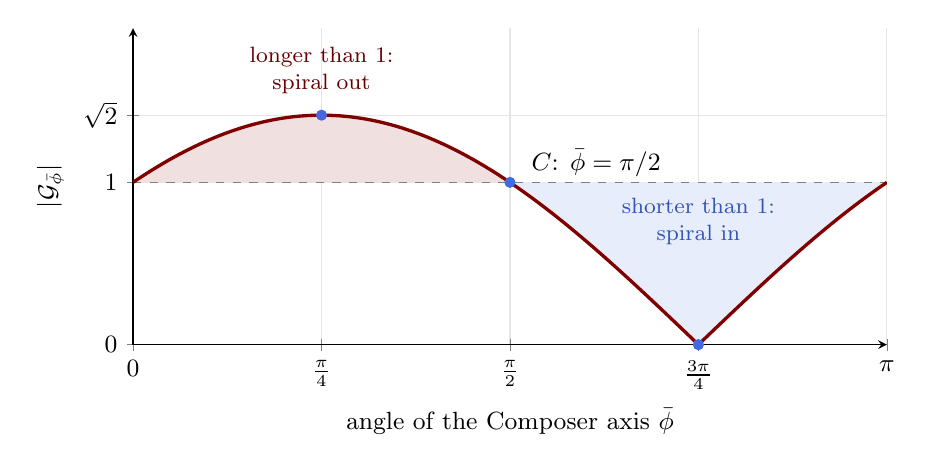
\begin{tikzpicture}
  \begin{axis}[
    width=0.92\textwidth, height=5.6cm,
    xmin=0, xmax=3.1416, ymin=0, ymax=1.95,
    xtick={0,0.7854,1.5708,2.3562,3.1416},
    xticklabels={$0$,$\frac{\pi}{4}$,$\frac{\pi}{2}$,$\frac{3\pi}{4}$,$\pi$},
    ytick={0,1,1.4142}, yticklabels={$0$,$1$,$\sqrt{2}$},
    xlabel={angle of the Composer axis $\bar{\phi}$}, ylabel={$|\mathcal{G}_{\bar{\phi}}|$},
    axis lines=left, grid=major, grid style={gray!20},
    tick label style={font=\small}, label style={font=\small}]
    % where the length is above 1 the powers spiral out, where it is below 1 they spiral in
    \fill[Maroon!12] plot[domain=0:90, samples=60] ({rad(\x)}, {sqrt(2)*sin(\x+45)}) -- cycle;
    \fill[RoyalBlue!12] plot[domain=90:180, samples=90] ({rad(\x)}, {abs(sqrt(2)*sin(\x+45))}) -- (3.1416,1) -- (1.5708,1) -- cycle;
    \draw[gray, dashed] (0,1) -- (3.1416,1);
    \addplot[very thick, Maroon, samples=200, domain=0:3.1416] {abs(sqrt(2)*sin(deg(x) + 45))};
    \addplot[only marks, mark=*, mark size=1.8pt, RoyalBlue] coordinates {(0.7854,1.4142) (1.5708,1) (2.3562,0)};
    \node[font=\small, anchor=west] at (axis cs:1.62,1.12) {$\mathbb{C}$: $\bar{\phi} = \pi/2$};
    \node[font=\footnotesize, text=Maroon!80!black, align=center] at (axis cs:0.7854,1.69) {longer than $1$:\\ spiral out};
    \node[font=\footnotesize, text=RoyalBlue!80!black, align=center] at (axis cs:2.3562,0.76) {shorter than $1$:\\ spiral in};
  \end{axis}
\end{tikzpicture}
\caption[The length of the Composer Unit]{The length of the Composer Unit, $|\mathcal{G}_{\bar{\phi}}| = |\sqrt{2}\sin(\bar{\phi} + \pi/4)|$, as the angle $\bar{\phi}$ of the Composer axis goes from $0$ to $\pi$. Where it is longer than $1$ (red), the powers of the Composer Unit spiral out; where it is shorter than $1$ (blue), they spiral in (\Cref{fig:power-regimes}).}
\label{fig:amplitude}
\end{figure}


% keep what follows together: break the page here if fewer than 12 lines are left
\keepblock{12}
\subsection{Relative Planes}\label{subsubsec:relative-planes}

\begin{figure}[tb]
\myfloatalign
\begin{tikzpicture}[>=Stealth, scale=2.1, every node/.style={font=\small}]
  \draw[->, gray] (-1.3,0) -- (1.6,0) node[right] {real axis};
  \foreach \ang/\len/\lab in {30/1.366/{\pi/6}, 45/1.414/{\pi/4}, 60/1.366/{\pi/3}, 120/0.366/{2\pi/3}, 150/0.366/{5\pi/6}}
  {
    \draw[->, thick, Maroon!75] (0,0) -- (\ang:\len);
    \node at (\ang:{\len+0.2}) {$\lab$};
  }
  \draw[->, very thick, RoyalBlue] (0,0) -- (90:1) node[left=5pt, align=right, text=RoyalBlue] {$\pi/2$:\\ the complex plane};
  \fill (0,0) circle (0.9pt);
\end{tikzpicture}
\caption[A fan of relative planes]{A fan of relative planes. Each arrow is the Composer Unit $\mathcal{G}_{\bar{\phi}}$ of one relative plane, drawn at its angle $\bar{\phi}$ with its own length $|\mathcal{G}_{\bar{\phi}}|$. The upright arrow ($\bar{\phi} = \pi/2$, length $1$) is the imaginary unit $i$. At $\bar{\phi} = 3\pi/4$ the length is $0$.}
\label{fig:fan}
\end{figure}

\begin{definition}[Relative Plane within the General Number Plane]\label{def:relative-plane}
The General Number Plane $\GN$ is a two-dimensional numerical and geometric framework generated by the real axis and the Composer axis associated with the unit $\Gp$.

To work in a specific geometric realization, one fixes a projection angle $\pb \in [0, \pi)$. The resulting two-dimensional plane, denoted $\GNp$, is called a \emph{Relative Plane}.

Each Relative Plane represents a particular instance of the General Number Plane relative to the chosen angle $\pb$, providing a concrete reference frame for algebraic and geometric constructions.
\end{definition}

\begin{remark}[The Complex Plane as a Relative Plane]\label{rem:complex-relative}
Among all Relative Planes $\GNp$ within the General Number Plane $\GN$, the case $\pb = \pi/2$ recovers the classical complex plane:
\[
\mathbb{G}_{\pi/2} = \C, \qquad \mathcal{G}_{\pi/2} = i .
\]
This shows that the complex numbers are not separate from the General Number Plane; rather, they correspond to a particular Relative Plane with an orthogonal Composer axis.

Thus, every Relative Plane can be viewed as a generalization of the complex plane, and the classical complex system appears as a special instance within the broader framework.
\end{remark}

\begin{plainwords}
Picture a hand fan. Each blade is a Composer axis at its own angle $\pb$, with its own step length, and each blade defines its own relative plane $\GNp$ (\Cref{fig:fan}). The General Number Plane is the whole fan. The complex plane is one blade among the others, the one that stands exactly upright. A relative plane is also called a \emph{subgeneral plane}; the two names mean the same thing.
\end{plainwords}

%------------------------------------------------
\section{Properties of the Composer Unit}\label{sec:composer-properties}
%------------------------------------------------

We now have a whole fan of planes, one for each angle. A new number system earns our trust in two ways: it must give back the old system exactly, and it must show something new. This section checks both at two angles: with the Composer axis upright, where the complex numbers come back, and with the axis leaning, where the powers of \Cref{thm:powers} trace a spiral.

\subsection[Reduction to the Complex Numbers]{Reduction to the Complex Number System}\label{subsec:reduction}

\begin{theorem}[Classical Recovery]\label{thm:classical-recovery}
Let $\pb = \dfrac{\pi}{2}$. Then, the General Number Plane $\GN$ reduces to the classical complex plane $\C$, and the Composer Unit becomes the imaginary unit:
\[
\mathcal{G}_{\pi/2} = i
\]
\end{theorem}

\begin{proof}
When $\pb = \dfrac{\pi}{2}$, we compute:
\[
\mathcal{A}_{\pi/2} = \left|\sqrt{2}\sin\left(\frac{3\pi}{4}\right)\right| = \left|\sqrt{2} \cdot \frac{\sqrt{2}}{2}\right| = 1
\]
\[
\vec{u}_{\pi/2} = \cos\left(\frac{\pi}{2}\right)\xv + \sin\left(\frac{\pi}{2}\right)\yv = \yv
\]
Therefore:
\[
\mathcal{G}_{\pi/2} = 1 \cdot \yv = \yv = i
\]
\end{proof}

\begin{remark}[The Classical Case $\pb = \frac{\pi}{2}$]\label{rem:classical-case}
Let us consider the particular case $\pb = \frac{\pi}{2}$, where the Composer Unit $\Gp$ aligns with the classical imaginary unit $i$. From the previously defined structure:
\begin{align*}
\Gp &= \Ap \cdot \up, \quad \text{with } \Ap = \left|\sqrt{2}\sin\left(\pb + \frac{\pi}{4}\right)\right|, \\
\up &= \cos(\pb)\xv + \sin(\pb)\yv .
\end{align*}
For $\pb = \frac{\pi}{2}$, we compute:
\[
\mathcal{A}_{\pi/2} = \left|\sqrt{2}\sin\left(\frac{3\pi}{4}\right)\right| = 1, \qquad \vec{u}_{\pi/2} = \yv, \qquad \Rightarrow \qquad \mathcal{G}_{\pi/2} = \yv .
\]
Thus, successive powers yield:
\[
\mathcal{G}^2_{\pi/2} = -\xv, \qquad \mathcal{G}^3_{\pi/2} = -\yv, \qquad \mathcal{G}^4_{\pi/2} = \xv .
\]
This result reflects a complete rotation cycle of $90^\circ$ per power, analogous to the behavior of $i$ in complex analysis:
\[
i = \yv, \qquad i^2 = -1 = -\xv, \qquad i^3 = -i = -\yv, \qquad i^4 = 1 = \xv .
\]
\begin{center}
\begin{tabular}{lll}
\toprule
\tableheadline{Power} & \tableheadline{Result} & \tableheadline{Interpretation} \\
\midrule
$\mathcal{G}^1_{\pi/2}$ & $\yv$ & $90^\circ$ rotation from $\xv$ \\
$\mathcal{G}^2_{\pi/2}$ & $-\xv$ & $180^\circ$ rotation \\
$\mathcal{G}^3_{\pi/2}$ & $-\yv$ & $270^\circ$ rotation \\
$\mathcal{G}^4_{\pi/2}$ & $\xv$ & $360^\circ$ rotation (identity) \\
\bottomrule
\end{tabular}
\end{center}
This example confirms that, in the special orthogonal case, the Composer Unit $\Gp$ reproduces the same rotational algebra as the complex imaginary unit $i$, but within a geometric and coordinate-based interpretation.
\end{remark}

These are the four quarter turns of Chapter~\ref{ch:one-number} in new clothes (\Cref{fig:power-regimes}(b)): all of complex arithmetic lives inside the General Number Plane, in the relative plane $\mathbb{G}_{\pi/2}$.

\subsection{When the Composer Axis Leans}\label{subsec:leaning-case}

Now let the axis lean, and watch what the powers do. We take the angle $\pb = \pi/3$, the relative plane of \Cref{fig:graph-paper}(b), and follow the powers of the Composer Unit through one full turn.

\begin{remark}[Extended Non-Orthogonal Case $\pb = \frac{\pi}{3}$, Subgeneral Plane]\label{rem:pi-over-three}
Let us extend the Composer Unit computations for $\pb = \frac{\pi}{3}$ up to the 6th power to observe the full rotational cycle of this generalized structure.

\emph{Base definitions:}
\[
\mathcal{A}_{\pi/3} \approx 1.365, \qquad \vec{u}_{\pi/3} = \frac{1}{2}\xv + \frac{\sqrt{3}}{2}\yv
\]
\begin{center}
\begin{tabular}{llll}
\toprule
\tableheadline{Power} & \tableheadline{Expression} & \tableheadline{Approx. Result} & \tableheadline{Rotation Angle} \\
\midrule
$\mathcal{G}^1$ & $\mathcal{A} \cdot \vec{u}_{\pi/3}$ & $0.6825\xv + 1.182\yv$ & $60^\circ$ \\
$\mathcal{G}^2$ & $\mathcal{A}^2 \cdot \vec{u}_{2\pi/3}$ & $-0.932\xv + 1.614\yv$ & $120^\circ$ \\
$\mathcal{G}^3$ & $\mathcal{A}^3 \cdot \vec{u}_{\pi}$ & $-2.546\xv$ & $180^\circ$ \\
$\mathcal{G}^4$ & $\mathcal{A}^4 \cdot \vec{u}_{4\pi/3}$ & $-1.739\xv - 3.013\yv$ & $240^\circ$ \\
$\mathcal{G}^5$ & $\mathcal{A}^5 \cdot \vec{u}_{5\pi/3}$ & $2.377\xv - 4.121\yv$ & $300^\circ$ \\
$\mathcal{G}^6$ & $\mathcal{A}^6 \cdot \vec{u}_{2\pi}$ & $6.5\xv$ & $360^\circ$ \\
\bottomrule
\end{tabular}
\end{center}
We observe a full geometric cycle with $60^\circ$ steps. However, unlike the classical complex system where all magnitudes stay constant, the amplitude here evolves as a power of the base amplitude $\Ap$, leading to expanding spirals or contractions depending on the value of $\pb$. This supports the view that $\Gp$ defines a generalized number system with rotational and amplitude dynamics.
\end{remark}

The computation of Remark~\ref{rem:pi-over-three} works for any angle. Here it is for three more, $\pb = \pi/4$, $\pb = \pi/5$ and $\pb = \pi/6$, with the amplitude and the direction taken from the Axiom.

\begin{workedexample}[Worked example: the powers for $\pb = \pi/4$, $\pi/5$ and $\pi/6$]
\emph{The angle $\pb = \pi/4$.} Here $\mathcal{A}_{\pi/4} = \left|\tfrac{\sqrt{2}}{2} + \tfrac{\sqrt{2}}{2}\right| = \sqrt{2}$ and $\vec{u}_{\pi/4} = \tfrac{\sqrt{2}}{2}\xv + \tfrac{\sqrt{2}}{2}\yv$, so the first power is $\mathcal{G}^1 = \xv + \yv$. Every result is exact: each power turns the arrow by another $45^\circ$ and stretches it by $\sqrt{2}$, and after eight steps it is back on the real axis, sixteen times longer than the unit.
\begin{center}
\small
\begin{tabular}{llll}
\toprule
\tableheadline{Power} & \tableheadline{Expression} & \tableheadline{Result} & \tableheadline{Rotation Angle} \\
\midrule
$\mathcal{G}^1$ & $\mathcal{A} \cdot \vec{u}_{\pi/4}$ & $\xv + \yv$ & $45^\circ$ \\
$\mathcal{G}^2$ & $\mathcal{A}^2 \cdot \vec{u}_{\pi/2}$ & $2\yv$ & $90^\circ$ \\
$\mathcal{G}^3$ & $\mathcal{A}^3 \cdot \vec{u}_{3\pi/4}$ & $-2\xv + 2\yv$ & $135^\circ$ \\
$\mathcal{G}^4$ & $\mathcal{A}^4 \cdot \vec{u}_{\pi}$ & $-4\xv$ & $180^\circ$ \\
$\mathcal{G}^5$ & $\mathcal{A}^5 \cdot \vec{u}_{5\pi/4}$ & $-4\xv - 4\yv$ & $225^\circ$ \\
$\mathcal{G}^6$ & $\mathcal{A}^6 \cdot \vec{u}_{3\pi/2}$ & $-8\yv$ & $270^\circ$ \\
$\mathcal{G}^7$ & $\mathcal{A}^7 \cdot \vec{u}_{7\pi/4}$ & $8\xv - 8\yv$ & $315^\circ$ \\
$\mathcal{G}^8$ & $\mathcal{A}^8 \cdot \vec{u}_{2\pi}$ & $16\xv$ & $360^\circ$ \\
\bottomrule
\end{tabular}
\end{center}
\emph{The angle $\pb = \pi/5$.} Here $\cos(\pi/5) = \tfrac{1 + \sqrt{5}}{4} \approx 0.809$, which is half the golden ratio $(1 + \sqrt{5})/2$ (\Cref{app:gs-special}), and $\sin(\pi/5) \approx 0.588$, so $\mathcal{A}_{\pi/5} \approx 1.397$ and $\vec{u}_{\pi/5} \approx 0.809\xv + 0.588\yv$. Ten steps of $36^\circ$ bring the arrow back to the real axis. The results are rounded to three decimals. The golden ratio is followed through these powers in \citet[Remark~5.7]{DerrazGNPreprint2026}.
\begin{center}
\small
\begin{tabular}{llll}
\toprule
\tableheadline{Power} & \tableheadline{Expression} & \tableheadline{Approx. Result} & \tableheadline{Rotation Angle} \\
\midrule
$\mathcal{G}^1$ & $\mathcal{A} \cdot \vec{u}_{\pi/5}$ & $1.130\xv + 0.821\yv$ & $36^\circ$ \\
$\mathcal{G}^2$ & $\mathcal{A}^2 \cdot \vec{u}_{2\pi/5}$ & $0.603\xv + 1.856\yv$ & $72^\circ$ \\
$\mathcal{G}^3$ & $\mathcal{A}^3 \cdot \vec{u}_{3\pi/5}$ & $-0.842\xv + 2.592\yv$ & $108^\circ$ \\
$\mathcal{G}^4$ & $\mathcal{A}^4 \cdot \vec{u}_{4\pi/5}$ & $-3.080\xv + 2.237\yv$ & $144^\circ$ \\
$\mathcal{G}^5$ & $\mathcal{A}^5 \cdot \vec{u}_{\pi}$ & $-5.317\xv$ & $180^\circ$ \\
$\mathcal{G}^6$ & $\mathcal{A}^6 \cdot \vec{u}_{6\pi/5}$ & $-6.009\xv - 4.365\yv$ & $216^\circ$ \\
$\mathcal{G}^7$ & $\mathcal{A}^7 \cdot \vec{u}_{7\pi/5}$ & $-3.206\xv - 9.866\yv$ & $252^\circ$ \\
$\mathcal{G}^8$ & $\mathcal{A}^8 \cdot \vec{u}_{8\pi/5}$ & $4.478\xv - 13.781\yv$ & $288^\circ$ \\
$\mathcal{G}^9$ & $\mathcal{A}^9 \cdot \vec{u}_{9\pi/5}$ & $16.375\xv - 11.897\yv$ & $324^\circ$ \\
$\mathcal{G}^{10}$ & $\mathcal{A}^{10} \cdot \vec{u}_{2\pi}$ & $28.272\xv$ & $360^\circ$ \\
\bottomrule
\end{tabular}
\end{center}
\emph{The angle $\pb = \pi/6$.} Here $\mathcal{A}_{\pi/6} = \tfrac{\sqrt{3}}{2} + \tfrac{1}{2} \approx 1.366$, the same length as $\mathcal{A}_{\pi/3}$ (Remark~\ref{rem:pi-over-three} gives it as $1.365$; \Cref{sec:two-roots-math} explains why two angles share one length), and $\vec{u}_{\pi/6} = \tfrac{\sqrt{3}}{2}\xv + \tfrac{1}{2}\yv$. The arrow now turns by only $30^\circ$ at each step, so it needs twelve steps to come back to the real axis, and it keeps growing all the way. The results are rounded to three decimals.
\begin{center}
\small
\begin{tabular}{llll}
\toprule
\tableheadline{Power} & \tableheadline{Expression} & \tableheadline{Approx. Result} & \tableheadline{Rotation Angle} \\
\midrule
$\mathcal{G}^1$ & $\mathcal{A} \cdot \vec{u}_{\pi/6}$ & $1.183\xv + 0.683\yv$ & $30^\circ$ \\
$\mathcal{G}^2$ & $\mathcal{A}^2 \cdot \vec{u}_{\pi/3}$ & $0.933\xv + 1.616\yv$ & $60^\circ$ \\
$\mathcal{G}^3$ & $\mathcal{A}^3 \cdot \vec{u}_{\pi/2}$ & $2.549\yv$ & $90^\circ$ \\
$\mathcal{G}^4$ & $\mathcal{A}^4 \cdot \vec{u}_{2\pi/3}$ & $-1.741\xv + 3.016\yv$ & $120^\circ$ \\
$\mathcal{G}^5$ & $\mathcal{A}^5 \cdot \vec{u}_{5\pi/6}$ & $-4.119\xv + 2.378\yv$ & $150^\circ$ \\
$\mathcal{G}^6$ & $\mathcal{A}^6 \cdot \vec{u}_{\pi}$ & $-6.498\xv$ & $180^\circ$ \\
$\mathcal{G}^7$ & $\mathcal{A}^7 \cdot \vec{u}_{7\pi/6}$ & $-7.687\xv - 4.438\yv$ & $210^\circ$ \\
$\mathcal{G}^8$ & $\mathcal{A}^8 \cdot \vec{u}_{4\pi/3}$ & $-6.062\xv - 10.500\yv$ & $240^\circ$ \\
$\mathcal{G}^9$ & $\mathcal{A}^9 \cdot \vec{u}_{3\pi/2}$ & $-16.563\yv$ & $270^\circ$ \\
$\mathcal{G}^{10}$ & $\mathcal{A}^{10} \cdot \vec{u}_{5\pi/3}$ & $11.312\xv - 19.594\yv$ & $300^\circ$ \\
$\mathcal{G}^{11}$ & $\mathcal{A}^{11} \cdot \vec{u}_{11\pi/6}$ & $26.766\xv - 15.453\yv$ & $330^\circ$ \\
$\mathcal{G}^{12}$ & $\mathcal{A}^{12} \cdot \vec{u}_{2\pi}$ & $42.219\xv$ & $360^\circ$ \\
\bottomrule
\end{tabular}
\end{center}
\end{workedexample}

\begin{figure}[tb]
\myfloatalign
% ================= (a) phi = pi/3, the values of Remark 3.7 =================
\begin{minipage}[b]{0.48\textwidth}
\centering
\begin{tikzpicture}[>=Stealth, every node/.style={font=\scriptsize}]
  \def\s{0.52}                                % centimetres per unit of length
  \draw[->, gray] (-1.45,0) -- (3.75,0);
  \draw[gray] (0,-2.3) -- (0,1.05);
  \draw[thick, Maroon!70, smooth, domain=0:360, samples=150, variable=\t] plot (\t:{\s*1.365^(\t/60)});
  \foreach \px/\py/\lab/\pos in {0.6825/1.182/{\mathcal{G}^1}/{above right}, -0.932/1.614/{\mathcal{G}^2}/{above left}, -2.546/0/{\mathcal{G}^3}/{above left}, -1.739/-3.013/{\mathcal{G}^4}/{below left}, 2.377/-4.121/{\mathcal{G}^5}/{below right}, 6.5/0/{\mathcal{G}^6}/{above}}
  {
    \draw[->, RoyalBlue!80] (0,0) -- ({\px*\s},{\py*\s});
    \fill[RoyalBlue] ({\px*\s},{\py*\s}) circle (1.3pt) node[\pos, inner sep=1.5pt] {$\lab$};
  }
\end{tikzpicture}

\smallskip
{\small (a) $\pb = \pi/3$ (Remark~\ref{rem:pi-over-three}): six steps of $60^\circ$, back at about $6.5$\par}
\end{minipage}\hfill
% ================= (b) phi = pi/4 =================
\begin{minipage}[b]{0.48\textwidth}
\centering
\begin{tikzpicture}[>=Stealth, every node/.style={font=\scriptsize}]
  \def\s{0.235}                               % centimetres per unit of length
  \draw[->, gray] (-1.15,0) -- (4.2,0);
  \draw[gray] (0,-2.25) -- (0,0.8);
  \draw[thick, Maroon!70, smooth, domain=0:360, samples=120, variable=\t] plot (\t:{\s*1.41421^(\t/45)});
  \foreach \px/\py/\lab/\pos in {1/1/{\mathcal{G}^1}/{right}, 0/2/{\mathcal{G}^2}/{above right}, -2/2/{\mathcal{G}^3}/{above left}, -4/0/{\mathcal{G}^4}/{above left}, -4/-4/{\mathcal{G}^5}/{below left}, 0/-8/{\mathcal{G}^6}/{below left}, 8/-8/{\mathcal{G}^7}/{below right}, 16/0/{\mathcal{G}^8}/{above}}
  {
    \draw[->, RoyalBlue!80] (0,0) -- ({\px*\s},{\py*\s});
    \fill[RoyalBlue] ({\px*\s},{\py*\s}) circle (1.3pt) node[\pos, inner sep=1.5pt] {$\lab$};
  }
\end{tikzpicture}

\smallskip
{\small (b) $\pb = \pi/4$: eight steps of $45^\circ$, back at exactly $16$\par}
\end{minipage}

\bigskip
% ================= (c) phi = pi/5 =================
\begin{minipage}[b]{0.48\textwidth}
\centering
\begin{tikzpicture}[>=Stealth, every node/.style={font=\scriptsize}]
  \def\s{0.14}                                % centimetres per unit of length
  \draw[->, gray] (-1.05,0) -- (4.3,0);
  \draw[gray] (0,-2.3) -- (0,0.7);
  \draw[thick, Maroon!70, smooth, domain=0:360, samples=150, variable=\t] plot (\t:{\s*1.39680^(\t/36)});
  \foreach \n in {1,...,10} {
    \pgfmathsetmacro{\rad}{\s*1.39680^\n}
    \ifnum\n>3 \draw[->, RoyalBlue!80] (0,0) -- ({36*\n}:\rad); \fi
    \fill[RoyalBlue] ({36*\n}:\rad) circle (1.1pt);
  }
  \node[above left, inner sep=1.5pt] at (144:{\s*3.80659}) {$\mathcal{G}^{4}$};
  \node[left, inner sep=1.5pt] at (180:{\s*5.31710}) {$\mathcal{G}^{5}$};
  \node[below left, inner sep=1.5pt] at (216:{\s*7.42693}) {$\mathcal{G}^{6}$};
  \node[below left, inner sep=1.5pt] at (252:{\s*10.37402}) {$\mathcal{G}^{7}$};
  \node[below, inner sep=1.5pt] at (288:{\s*14.49040}) {$\mathcal{G}^{8}$};
  \node[below right, inner sep=1.5pt] at (324:{\s*20.24023}) {$\mathcal{G}^{9}$};
  \node[above, inner sep=1.5pt] at (0:{\s*28.27153}) {$\mathcal{G}^{10}$};
\end{tikzpicture}

\smallskip
{\small (c) $\pb = \pi/5$: ten steps of $36^\circ$, back at about $28.3$\par}
\end{minipage}\hfill
% ================= (d) phi = pi/6 =================
\begin{minipage}[b]{0.48\textwidth}
\centering
\begin{tikzpicture}[>=Stealth, every node/.style={font=\scriptsize}]
  \def\s{0.095}                               % centimetres per unit of length
  \draw[->, gray] (-1.0,0) -- (4.5,0);
  \draw[gray] (0,-2.3) -- (0,0.6);
  \draw[thick, Maroon!70, smooth, domain=0:360, samples=160, variable=\t] plot (\t:{\s*1.36603^(\t/30)});
  \foreach \n in {1,...,12} {
    \pgfmathsetmacro{\rad}{\s*1.36603^\n}
    \ifnum\n>4 \draw[->, RoyalBlue!80] (0,0) -- ({30*\n}:\rad); \fi
    \fill[RoyalBlue] ({30*\n}:\rad) circle (1.1pt);
  }
  \node[above left, inner sep=1.5pt] at (180:{\s*6.49760}) {$\mathcal{G}^{6}$};
  \node[left, inner sep=1.5pt] at (210:{\s*8.87588}) {$\mathcal{G}^{7}$};
  \node[below left, inner sep=1.5pt] at (240:{\s*12.12468}) {$\mathcal{G}^{8}$};
  \node[below left, inner sep=1.5pt] at (270:{\s*16.56262}) {$\mathcal{G}^{9}$};
  \node[below, inner sep=1.5pt] at (300:{\s*22.62496}) {$\mathcal{G}^{10}$};
  \node[below right, inner sep=1.5pt] at (330:{\s*30.90627}) {$\mathcal{G}^{11}$};
  \node[above, inner sep=1.5pt] at (0:{\s*42.21874}) {$\mathcal{G}^{12}$};
\end{tikzpicture}

\smallskip
{\small (d) $\pb = \pi/6$: twelve steps of $30^\circ$, back at about $42.2$\par}
\end{minipage}
\caption[The spiral of powers]{The spiral of powers for four angles. Each power of the Composer Unit turns by another $\bar{\phi}$ and grows by the factor $\mathcal{A}_{\pi/3} \approx 1.365$ in (a), $\mathcal{A}_{\pi/4} = \sqrt{2}$ in (b) and $\mathcal{A}_{\pi/5} \approx 1.397$ in (c); in (d) the factor is the same as in (a), but the steps are only $30^\circ$. The points are the values of Remark~\ref{rem:pi-over-three} and of the worked example; the curves join them. Each panel has its own scale; the first powers in (c) and (d) are too close to $0$ to be labelled.}
\label{fig:spiral}
\end{figure}

% keep what follows together: break the page here if fewer than 10 lines are left
\keepblock{10}
\begin{plainwords}
In the complex plane, the powers of $i$ walk around a circle: four steps and you are home. In the relative plane at $\pb = \pi/3$, the powers of the Composer Unit also come home to the real axis, after six steps of $60^\circ$ each, but they come home \emph{bigger}. Their path is a spiral that opens outwards (\Cref{fig:spiral}), and the smaller the angle, the more steps the trip takes and the bigger the powers are when they come home.
\end{plainwords}

The spiral is proved for every angle in \citet[Proposition~5.6]{DerrazGNPreprint2026}. The powers show what the Composer Unit does to itself. The next section asks a more practical question: given any General Number, how far is it from zero, and in which direction does it point?

%------------------------------------------------
\section[General Numbers and General Trigonometry]{General Numbers and General\\ Trigonometry Functions}\label{sec:gn-trig}
%------------------------------------------------

We now bring together the two halves of Part~\ref{pt:beyond}. In Chapter~\ref{ch:oblique}, the General Sinus gave us two coordinates, $\cos(\alpha, \phi)$ and $\sin(\alpha, \phi)$, for reading a point along the real axis and along a leaning axis. In this chapter, the General Number Plane gave us numbers whose two parts are measured along exactly such axes. The two ideas fit together like a key in a lock.

\subsection{A Polar Form with Two Angles}\label{subsec:two-angle-polar}

In the complex plane, a number is fixed by its length and one angle. In a relative plane, where the second axis leans, the natural description uses two.

\begin{definition}[General Scalar Representation with Generalized Trigonometric Functions]\label{def:general-polar}
In the General Number Plane $\GN$, any element
\[
z = a + b\Gp
\]
can be represented using a generalized polar form, where the real part $a$ and the Composer part $b\Gp$ are expressed in terms of a magnitude $M$ and generalized trigonometric functions that depend on two angles: the projection angle $\phi$ and a studied angle $\alpha$:
\[
a = M \cdot \cos(\alpha, \phi), \qquad b\Gp = M \cdot \sin(\alpha, \phi) .
\]
\end{definition}

\subsection{The Triangle of a General Number}\label{subsec:gn-triangle}

Walk from the origin $O$ to $z$ in two legs: first $a$ along the real axis, to the corner $P$, then $b$ steps along the Composer axis, to the tip $Q$, which is the number $z$ itself. The two legs and the base $OQ$ form a triangle, and the next two theorems read its sides and its angles.

\begin{theorem}[Triangle Interpretation and Magnitude Formula]\label{thm:triangle}
Let $z = a + b\Gp$ be a General Number in the Subgeneral Plane defined by angle $\pb$. Then, one can associate $z$ with a triangle where:
\begin{itemize}
  \item The side opposite to angle $\alpha$ represents the \textbf{Composer part} $b\Gp$,
  \item The side opposite to angle $\phi$ represents the \textbf{Real part} $a$,
  \item The base of the triangle is the \textbf{Magnitude} $M$.
\end{itemize}
Applying the Law of Cosines to this triangle, the magnitude $M$ satisfies:
\[
M^2 = a^2 + b^2\Gp^2 + 2ab\cos(\pb)\Gp .
\]
\end{theorem}

% keep what follows together: break the page here if fewer than 11 lines are left
\keepblock{11}
\begin{theorem}[Phase Angle Expression in the General Number Plane]\label{thm:phase}
Let $z = a + b\Gp$ be a General Number where $a \neq 0$:
\[
\alpha = k\pi + \beta, \qquad \text{where} \quad \beta = \arctan\left(\frac{\eta\sin(\pb)}{1 + \eta\cos(\pb)}\right),
\]
with $k \in \Z$, $\eta = \Gp\dfrac{b}{a}$, and $\pb \in [0, \pi)$.

Moreover, the complementary angle between the Composer axis and the vector is:
\[
\phi = \pb - \alpha .
\]
\end{theorem}

\begin{figure}[tb]
\myfloatalign
\begin{tikzpicture}[>=Stealth, scale=1.35, every node/.style={font=\small}]
  \coordinate (O) at (0,0);
  \coordinate (P) at (2.3,0);
  \coordinate (Q) at ($(P)+(60:1.6)$);
  \coordinate (X) at (4.2,0);
  \draw[->, gray] (-0.3,0) -- (4.3,0) node[right] {real axis};
  \draw[gray, dashed] (P) -- ($(P)+(60:2.3)$) node[above] {Composer axis direction};
  \draw[very thick, Maroon!85!black] (O) -- (P) node[midway, below] {$a$ (real part)};
  \draw[very thick, RoyalBlue] (P) -- (Q) node[midway, right] {$b\,\mathcal{G}_{\bar{\phi}}$ (Composer part)};
  \draw[very thick] (O) -- (Q) node[midway, above left] {$M$ (magnitude)};
  \pic [draw, "$\alpha$", angle radius=0.8cm, angle eccentricity=1.25] {angle = P--O--Q};
  \pic [draw, "$\phi$", angle radius=0.55cm, angle eccentricity=1.4] {angle = O--Q--P};
  \pic [draw, gray, "$\bar{\phi}$", angle radius=0.45cm, angle eccentricity=1.5] {angle = X--P--Q};
  \fill (O) circle (1.3pt) node[below left] {$O$};
  \fill (P) circle (1.3pt) node[below] {$P$};
  \fill (Q) circle (1.5pt) node[above right] {$Q$: $z = a + b\,\mathcal{G}_{\bar{\phi}}$};
\end{tikzpicture}
\caption[The triangle of a General Number]{The triangle of a General Number (Theorem~\ref{thm:triangle}): the real part runs from $O$ to $P$, the Composer part from $P$ to $Q$, and the magnitude $M$ joins $O$ to $Q$.}
\label{fig:gn-triangle}
\end{figure}

\begin{plainwords}
Look at \Cref{fig:gn-triangle} and compare it with the oblique triangle of Chapter~\ref{ch:oblique}. It is the same triangle. The studied angle $\alpha$ sits at the origin $O$, the projection angle $\phi$ sits at the tip $Q$, and the leaning axis makes the angle $\pb = \alpha + \phi$ with the real axis. The General Sinus therefore reads the two parts of a General Number directly: the real part is $M\cos(\alpha, \phi)$ and the Composer part is $M\sin(\alpha, \phi)$.

In the two formulas of the theorems, the Composer Unit enters through its length, the amplitude $\Ap$: the side of the triangle opposite $\alpha$ is made of $b$ steps of that length. With this in mind, \Cref{thm:triangle} is the law of cosines of the triangle, and \Cref{thm:phase} gives the angle at the origin from the ratio $\eta$ of the two walks.
\end{plainwords}

\subsection{Two Worked Examples}\label{subsec:gn-examples}

The first example tries the formulas on familiar ground, in the complex plane. The second puts them to work in a plane that leans, and \Cref{fig:leaning-example} draws it to scale.

\begin{workedexample}[Worked example 1: the complex plane again]
Take $\pb = \pi/2$, where $\mathcal{G}_{\pi/2} = i$ has length $1$ and $\cos(\pi/2) = 0$. \Cref{thm:triangle} becomes
\[
M^2 = a^2 + b^2 ,
\]
the theorem of Pythagoras, which gives the usual modulus of $a + bi$. \Cref{thm:phase} becomes $\beta = \arctan(\eta)$ with $\eta = b/a$, the usual argument of a complex number. The geometry of the complex plane is found again.
\end{workedexample}

\begin{workedexample}[Worked example 2: a number that leans]
Take $\pb = \pi/3$ and the General Number $z = 1 + 1 \cdot \mathcal{G}_{\pi/3}$, so $a = 1$ and $b = 1$. Use the rounded length of Remark~\ref{rem:pi-over-three}, $\mathcal{A}_{\pi/3} \approx 1.365$, and $\cos(\pi/3) = 0.5$.
\begin{itemize}
  \item Magnitude, by \Cref{thm:triangle}: $M^2 \approx 1 + 1.365^2 + 2 \cdot 0.5 \cdot 1.365 \approx 1 + 1.863 + 1.365 = 4.228$, so $M \approx 2.056$.
  \item Phase angle, by \Cref{thm:phase}: $\eta \approx 1.365$, so $\beta = \arctan\bigl(1.365 \cdot 0.866 / (1 + 1.365 \cdot 0.5)\bigr) \approx \arctan(0.703) \approx 35.1^\circ$, and $\phi = 60^\circ - 35.1^\circ \approx 24.9^\circ$.
  \item Check with the General Sinus, by Definition~\ref{def:general-polar}: $M\cos(\alpha, \phi) = M \sin(\phi)/\sin(\pb) \approx 2.056 \cdot 0.421 / 0.866 \approx 1.00$, which is the real part $a$; and $M \sin(\alpha, \phi) = M\sin(\alpha)/\sin(\pb) \approx 2.056 \cdot 0.575/0.866 \approx 1.365$, which is the length of the Composer part.
\end{itemize}
The three statements of this section agree, as they should: they are three views of one triangle.
\end{workedexample}

\begin{figure}[htb]
\myfloatalign
\begin{tikzpicture}[>=Stealth, every node/.style={font=\small}]
  \def\s{2.3}                                   % centimetres per unit of length
  \coordinate (O) at (0,0);
  \coordinate (P) at (\s,0);                     % a = 1
  \coordinate (Q) at ($(P)+(60:{1.365*\s})$);     % one step of the Composer Unit, about 1.365 long
  \coordinate (X) at ({2.5*\s},0);
  \fill[RoyalBlue!7] (O) -- (P) -- (Q) -- cycle;
  \draw[->, gray] (-0.3,0) -- ({2.65*\s},0) node[below left] {real axis};
  \draw[gray, dashed] (P) -- ($(P)+(60:{1.7*\s})$) node[above, font=\footnotesize] {Composer axis};
  \draw[very thick, Maroon!85!black] (O) -- (P) node[midway, below] {$a = 1$};
  \draw[very thick, RoyalBlue] (P) -- (Q) node[midway, right=1pt] {$b\,\mathcal{A}_{\pi/3} \approx 1.365$};
  \draw[very thick] (O) -- (Q) node[midway, above left] {$M \approx 2.056$};
  \pic [draw, "$\alpha$", angle radius=1.05cm, angle eccentricity=1.22] {angle = P--O--Q};
  \pic [draw, "$\phi$", angle radius=0.8cm, angle eccentricity=1.28] {angle = O--Q--P};
  \pic [draw, gray, "$\pb$", angle radius=0.45cm, angle eccentricity=1.55] {angle = X--P--Q};
  \fill (O) circle (1.3pt) node[below left] {$0$};
  \fill (Q) circle (1.5pt) node[above left] {$z = 1 + 1 \cdot \mathcal{G}_{\pi/3}$};
  \node[anchor=west, align=left, font=\footnotesize] at ({2.05*\s},{1.02*\s}) {$\alpha \approx 35.1^\circ$\\ $\phi \approx 24.9^\circ$\\ $\alpha + \phi = \pb = 60^\circ$};
\end{tikzpicture}
\caption[A number that leans, drawn to scale]{Worked example 2 drawn to scale. The number $z = 1 + 1 \cdot \mathcal{G}_{\pi/3}$ is one step along the real axis and one step of the Composer Unit, about $1.365$ long. The base is $M \approx 2.056$, and the angles $\alpha \approx 35.1^\circ$ and $\phi \approx 24.9^\circ$ add up to $\pb = 60^\circ$.}
\label{fig:leaning-example}
\end{figure}

%------------------------------------------------
\section{The Parts of a General Number}\label{sec:gn-words}
%------------------------------------------------

With the numbers built, the chapter turns to the words that Part~\ref{pt:foundations} will use. \Cref{subsec:gn-definitions} met the two parts of a General Number informally; here they get their exact names, together with the rule for when two numbers are equal and the place of the General Numbers among the older numbers.

\subsection{Real Part, Composer Part and Equality}\label{subsec:gn-parts}

\begin{figure}[tb]
\myfloatalign
\begin{minipage}[b]{0.62\textwidth}
\centering
\begin{tikzpicture}[>=Stealth, every node/.style={font=\footnotesize}]
  \def\s{1.5}
  \coordinate (O) at (0,0);
  \coordinate (P) at ({2*\s},0);
  \coordinate (Q) at ($(P)+(60:{1.36603*\s})$);
  \draw[->, gray] (-0.3,0) -- ({3.25*\s},0) node[right] {real axis};
  \draw[gray, dashed] (O) -- (60:{1.6*\s}) node[above] {Composer axis};
  \draw[gray] (0.45,0) arc (0:60:0.45);
  \node[gray] at (30:0.7) {$\pb$};
  \draw[gray, densely dotted] (Q) -- (Q |- O);
  \draw[->, very thick, Maroon] (O) -- (P);
  \draw[->, very thick, RoyalBlue] (P) -- (Q);
  \node[RoyalBlue!85!black, anchor=west] at ($(P)!0.45!(Q)+(0.14,-0.06)$) {$\Com(z) = \mathcal{G}_{\pi/3}$};
  \draw[->, thin] (O) -- (Q);
  \fill (Q) circle (1.6pt) node[above] {$z$};
  % the two readings on the real axis
  \draw[|-|, Maroon] (0,-0.36) -- ({2*\s},-0.36) node[midway, below] {real part $\Re(z) = 2$};
  \draw[|-|, gray!70!black] (0,-0.92) -- ({2.68301*\s},-0.92) node[midway, below] {shadow $\Sh(z) \approx 2.683$};
\end{tikzpicture}

\smallskip
{\small (a) $z = 2 + \mathcal{G}_{\pi/3}$ and its two parts\par}
\end{minipage}\hfill
\begin{minipage}[b]{0.34\textwidth}
\centering
\begin{tikzpicture}[>=Stealth, every node/.style={font=\footnotesize}]
  \def\s{1.05}
  \draw[->, gray] (-0.2,0) -- ({3.45*\s},0);
  \foreach \x in {0,1,2,3} {
    \draw[gray] ({\x*\s},-0.07) -- ({\x*\s},0.07);
    \node[gray!80!black, below] at ({\x*\s},-0.07) {$\x$};
  }
  \draw[->, very thick, Maroon] (0,1.3) -- ({2*\s},1.3);
  \draw[->, very thick, RoyalBlue] ({2*\s},1.3) -- ({3*\s},1.3);
  \node[anchor=south west, inner sep=1pt] at (0,1.37) {$2 + 1 \cdot \mathcal{G}_0$};
  \draw[->, very thick, Maroon] (0,0.55) -- ({1*\s},0.55);
  \draw[->, very thick, RoyalBlue] ({1*\s},0.55) -- ({3*\s},0.55);
  \node[anchor=south west, inner sep=1pt] at (0,0.62) {$1 + 2\,\mathcal{G}_0$};
  \draw[gray, densely dotted] ({3*\s},1.3) -- ({3*\s},0);
  \fill ({3*\s},0) circle (1.6pt);
\end{tikzpicture}

\smallskip
{\small (b) $\pb = 0$: a line, no plane\par}
\end{minipage}
\caption[A General Number and its parts]{A General Number and its parts. (a) In the relative plane at $\pi/3$, the number $z = 2 + \mathcal{G}_{\pi/3}$ is its real part $\Re(z) = 2$ (dark red) followed by its Composer part $\Com(z) = \mathcal{G}_{\pi/3}$, one step of the Composer Unit, about $1.366$ long (blue). Its two readings on the real axis are the real part, $2$, and the shadow, about $2.683$ (Remark~\ref{rem:part-shadow}). (b) At the angle $0$ the Composer Unit is $\mathcal{G}_0 = 1$, and the walks $1 + 2\,\mathcal{G}_0$ and $2 + 1 \cdot \mathcal{G}_0$ end at the same point, $3$ (Remark~\ref{rem:line-no-plane}).}
\label{fig:gn-parts}
\end{figure}

\begin{definition}[Real Part, Composer Part and Composer Coordinate]\label{def:gn-parts}
Let $z = a + b\Gp$ be a General Number of the relative plane $\GNp$, with $a, b \in \R$.
\begin{itemize}
  \item The real number $a$ is the \emph{real part} of $z$, written $\Re(z) = a$.
  \item The term $b\Gp$ is the \emph{Composer part} of $z$, written $\Com(z) = b\Gp$: it is $b$ steps of the Composer Unit along the Composer axis, an arrow of length $|b|\,\Ap$.
  \item The real number $b$, the number of those steps, is the \emph{Composer coordinate} of $z$.
\end{itemize}
Every General Number is the sum of its two parts:
\[
z = \Re(z) + \Com(z).
\]
\end{definition}

% keep what follows together: break the page here if fewer than 8 lines are left
\keepblock{8}
\begin{plainwords}
Why three names for two legs? In the complex plane the second leg of $a + bi$ is $|b|$ long, because $i$ has length one, so the number $b$ and the leg $bi$ hardly need two names. Here the step $\Gp$ has a length of its own, and the leg $b\Gp$ is $|b|\,\Ap$ long (\Cref{fig:gn-parts}(a)). That is why the Composer coordinate $b$ and the Composer part $b\Gp$ are named apart: it is the non-unified reference of Definition~\ref{def:non-unified}, in one line.
\end{plainwords}

\begin{definition}[Equality of General Numbers]\label{def:gn-equality}
Two General Numbers of the same relative plane, $z_1 = a_1 + b_1\Gp$ and $z_2 = a_2 + b_2\Gp$, are equal, $z_1 = z_2$, if and only if
\[
a_1 = a_2 \qquad \text{and} \qquad b_1 = b_2 ,
\]
that is, if and only if they have the same real part and the same Composer part.
\end{definition}

\begin{remark}[A Line, No Plane]\label{rem:line-no-plane}
Definition~\ref{def:gn-equality} agrees with the picture on the page as long as the Composer Unit leaves the real axis, that is, for $0 < \pb < \pi$ with $\Ap \neq 0$. Then the two axes meet at $0$ only, and every point of the page is reached by exactly one pair $(a, b)$: the relative plane is a \emph{true plane}. Two angles close it into a line.
\begin{itemize}
  \item At $\pb = 0$, $\mathcal{A}_0 = 1$ and $\vec{u}_0 = \xv$, so $\mathcal{G}_0 = 1$: the Composer axis lies on the real axis, and $1 + 2\,\mathcal{G}_0$ and $2 + 1 \cdot \mathcal{G}_0$ are the same number, $3$, although their parts differ.
  \item At $\pb = 3\pi/4$, $\mathcal{A}_{3\pi/4} = 0$, so $\mathcal{G}_{3\pi/4} = 0$, and every General Number is its own real part.
\end{itemize}
In both cases the relative plane is \emph{a line, no plane}. Every other angle gives a true plane, and every relative plane in this book is a true plane unless the angle $0$ is named on purpose.
\end{remark}

\subsection{The Set of General Numbers and the Ladder}\label{subsec:gn-ladder}

\begin{definition}[The Set of General Numbers]\label{def:gn-set}
The set of all General Numbers, of every relative plane, is written $\GN$:
\[
\GN = \bigcup_{\pb \in [0, \pi)} \GNp .
\]
General Numbers are added, multiplied and compared within one relative plane, with one Composer Unit.
\end{definition}

\begin{proposition}[The Ladder of Number Sets]\label{prop:ladder}
As the counting numbers are a subset of the integers, the complex numbers are a subset of the General Numbers:
\[
\mathbb{N} \subset \Z \subset \mathbb{Q} \subset \R \subset \C \subset \GN .
\]
\end{proposition}

\begin{proof}
The first four inclusions are the ladder of Chapter~\ref{ch:one-number} (\Cref{tab:ladder-small}). The last one is Remark~\ref{rem:complex-relative}: the complex plane is the relative plane $\mathbb{G}_{\pi/2}$, where $\mathcal{G}_{\pi/2} = i$ (\Cref{thm:classical-recovery}).
\end{proof}

\begin{remark}[Real Numbers and Pure Composer Numbers]\label{rem:gn-kinds}
A General Number with no Composer part, $\Com(z) = 0$, is a real number. The real numbers lie on the real axis, which all the relative planes share, so $\R$ lies inside every $\GNp$. A General Number with no real part, $\Re(z) = 0$, is a \emph{pure Composer number}, $z = b\Gp$; it lies on the Composer axis of its own relative plane. In the complex plane the pure Composer numbers are the imaginary numbers $bi$.
\end{remark}

\begin{figure}[tb]
\myfloatalign
\begin{tikzpicture}[every node/.style={font=\small}]
  \foreach \k/\sym/\col in {5/{\mathbb{G}}/Maroon, 4/{\mathbb{C}}/RoyalBlue!80!black, 3/{\mathbb{R}}/gray!75!black, 2/{\mathbb{Q}}/gray!75!black, 1/{\mathbb{Z}}/gray!75!black, 0/{\mathbb{N}}/gray!75!black} {
    \pgfmathsetmacro{\xa}{0.9 - 0.16*\k}
    \pgfmathsetmacro{\ya}{0.9 - 0.16*\k}
    \pgfmathsetmacro{\xb}{2.35 + 1.72*\k}
    \pgfmathsetmacro{\yb}{1.75 + 0.42*\k}
    \draw[rounded corners=4pt, thick, draw=\col] (\xa,\ya) rectangle (\xb,\yb);
    \node[anchor=north west, text=\col, inner sep=2.5pt] at (\xa,\yb) {$\sym$};
  }
  \node[font=\footnotesize] at (1.62,1.17) {$1, 2, 3$};
  \node[font=\footnotesize] at (3.21,1.45) {$-2$, $0$};
  \node[font=\footnotesize] at (4.93,1.58) {$\tfrac{1}{3}$, $-0.5$};
  \node[font=\footnotesize] at (6.65,1.72) {$\sqrt{2}$, $\pi$};
  \node[font=\footnotesize] at (8.37,1.85) {$i$, $1 + i$};
  \node[font=\footnotesize, align=center] at (10.09,1.98) {$\mathcal{G}_{\pi/3}$\\[3pt] $2 + \mathcal{G}_{\pi/4}$};
\end{tikzpicture}
\caption[The ladder of number sets]{The ladder of number sets (Proposition~\ref{prop:ladder}). Each set holds every set drawn inside it, and a few of its members are written in the ring that it adds: the counting numbers $\mathbb{N}$, the integers $\mathbb{Z}$, the fractions $\mathbb{Q}$, the real numbers $\mathbb{R}$, the complex numbers $\mathbb{C}$ and the General Numbers $\mathbb{G}$. The complex plane is one relative plane, $\mathbb{G}_{\pi/2}$; the outer ring holds the numbers of the leaning planes, such as $\mathcal{G}_{\pi/3}$ and $2 + \mathcal{G}_{\pi/4}$.}
\label{fig:ladder}
\end{figure}

\begin{plainwords}
The new rung keeps all the old rungs inside it (\Cref{fig:ladder}). What it adds is the freedom of the Composer axis to lean, with a step whose length depends on how far it leans. Note what is new and what is not: a true relative plane covers the same points of the page as the complex plane, so what is new is not the points but the frame in which they are named.
\end{plainwords}

%------------------------------------------------
\section{Sums, Products and Two Readings}\label{sec:gn-shadows}
%------------------------------------------------

Numbers are made to be added and multiplied. This section does both within one relative plane, and then reads the result on the real axis in two ways: by its shadow, a drop straight down, and by its real part, a walk back along the Composer axis. The second reading needs one new rule, the Rule of the Square, and it gives every product a real part with one fixed minus sign. The physical chapters read every measured force with it.

\subsection{Sum and Product}\label{subsec:gn-product}

\begin{definition}[Sum and Product]\label{def:gn-product}
Let $z_1 = a_1 + b_1\Gp$ and $z_2 = a_2 + b_2\Gp$ be General Numbers of one relative plane. Their sum is taken part by part,
\[
z_1 + z_2 = (a_1 + a_2) + (b_1 + b_2)\,\Gp ,
\]
and their product $z_1 z_2$ is the product of the two arrows by Wessel's rule: the lengths multiply and the angles add.
\end{definition}

\begin{proposition}[The Three Terms of a Product]\label{prop:three-terms}
The product of two General Numbers of one relative plane multiplies out like two brackets:
\[
z_1 z_2 = a_1 a_2 + (a_1 b_2 + b_1 a_2)\,\Gp + b_1 b_2\,\Gp^2 .
\]
The three terms are the \emph{real term} $a_1 a_2$, along the real axis; the \emph{cross term} $(a_1 b_2 + b_1 a_2)\,\Gp$, along the Composer axis, at the angle $\pb$; and the \emph{square term} $b_1 b_2\,\Gp^2$, along the arrow $\Gp^2$, of length $\Ap^2$ at the angle $2\pb$ (\Cref{thm:powers}).
\end{proposition}

\begin{proof}
Multiplying by a fixed arrow turns the whole page by its angle and stretches it by its length, and a turn and a stretch carry a sum of arrows to the sum of their images. So each part of $z_1$ multiplies each part of $z_2$. The four products are $a_1 a_2$, $a_1 b_2\,\Gp$, $b_1 a_2\,\Gp$ and $b_1 b_2\,\Gp\,\Gp = b_1 b_2\,\Gp^2$, and the two middle ones share the factor $\Gp$.
\end{proof}

In a true plane the sum and the product are arrows of the page, and so, by Remark~\ref{rem:line-no-plane}, they are again General Numbers of the same relative plane.

\subsection{The Shadow on the Real Axis}\label{subsec:gn-shadow}

\begin{definition}[The Shadow on the Real Axis]\label{def:shadow}
The \emph{shadow} of a General Number $z$ on the real axis, written $\Sh(z)$, is the signed length of its perpendicular projection on that axis: drop a perpendicular from the tip of $z$ to the real axis, and measure from $0$ to its foot, positive forward and negative backward. The tip of $z = a + b\Gp$ lies $a + b\,\Ap\cos(\pb)$ across and $b\,\Ap\sin(\pb)$ up, so
\[
\Sh(z) = a + b\,\Ap\cos(\pb).
\]
\end{definition}

\begin{theorem}[The Shadows of a Product]\label{thm:shadow-product}
In a relative plane $\GNp$:
\begin{enumerate}
  \item the shadow of a sum is the sum of the shadows, and $\Sh(c\,z) = c\,\Sh(z)$ for every real number $c$;
  \item $\Sh(\Gp^n) = \Ap^n\cos(n\pb)$ for every power of the Composer Unit;
  \item the product of two General Numbers has the shadow
  \[
  \Sh(z_1 z_2) = a_1 a_2 + (a_1 b_2 + b_1 a_2)\,\Ap\cos(\pb) + b_1 b_2\,\Ap^2\cos(2\pb).
  \]
\end{enumerate}
Each term of a product counts with the shadow of its direction: $1$ for the real term, $\cos(\pb)$ for the cross term and $\cos(2\pb)$ for the square term.
\end{theorem}

\begin{proof}
(1) Arrows placed head to tail add, and so do the feet of their perpendiculars; stretching an arrow by $c$ stretches its shadow by $c$. (2) By \Cref{thm:powers}, $\Gp^n$ has the length $\Ap^n$ and leans at $n\pb$, so the foot of its perpendicular lies at $\Ap^n\cos(n\pb)$. (3) Apply (1) and (2) to the three terms of Proposition~\ref{prop:three-terms}.
\end{proof}

\begin{remark}[Real Part and Shadow]\label{rem:part-shadow}
The real part and the shadow both read a General Number on the real axis, in two different ways. The real part $\Re(z) = a$ slides the tip of $z$ back to the real axis along the Composer axis; the shadow $\Sh(z) = a + b\,\Ap\cos(\pb)$ drops it straight down. The two differ by $b\,\Ap\cos(\pb)$, so they agree for real numbers and for every number of the complex plane, where the Composer axis stands upright, and nowhere else.
\end{remark}

\begin{plainwords}
Picture a lamp high above the real axis. The shadow of $z$ is where its tip falls under that lamp: the component of the arrow along the real axis, in the ordinary sense of geometry, and what a ruler laid along that axis would read. The real part counts steps in the leaning frame instead. For the number $z = 2 + \mathcal{G}_{\pi/3}$ of \Cref{fig:gn-parts}(a), the real part is $2$, while the shadow is $2 + 1.366 \times 0.5 \approx 2.683$.
\end{plainwords}

\subsection{The Real Part of a Product}\label{subsec:gn-real-product}

The product of Proposition~\ref{prop:three-terms} has three terms. The first two are already written in the form $a + b\Gp$: the real term is a real number, and the cross term is a number of steps of the Composer Unit. The third is not. It carries the square $\Gp^2$, an arrow that leans at the angle $2\pb$, and before a product can be read by its real part we must know the real part of that square. One rule gives it. Here $|\Gp|$ is the length of the Composer Unit, the amplitude $\Ap$ of Definition~\ref{def:non-unified}.

\begin{proposition}[The Rule of the Square]\label{prop:square-rule}
In every true plane, $0 < \pb < \pi$ with $\Gp \neq 0$, the square of the Composer Unit is the General Number
\[
\Gp^2 = 2\,|\Gp|\cos\pb\;\Gp - |\Gp|^2 ,
\]
with the real part $\Re(\Gp^2) = -|\Gp|^2$ and the Composer coordinate $2\,|\Gp|\cos\pb$.
\end{proposition}

\begin{proof}
By \Cref{thm:powers}, $\Gp^2$ is an arrow of length $|\Gp|^2$ at the angle $2\pb$, so its tip lies $|\Gp|^2\cos 2\pb$ across and $|\Gp|^2\sin 2\pb$ up. In a true plane it is reached by exactly one walk, $a$ steps along the real axis and then $b$ steps of the Composer Unit (Remark~\ref{rem:line-no-plane}). Only the leaning steps go up, each by $|\Gp|\sin\pb$, which is not zero; so
\[
b = \frac{|\Gp|^2\sin 2\pb}{|\Gp|\sin\pb} = 2\,|\Gp|\cos\pb .
\]
Those steps also carry the walk across by $b\,|\Gp|\cos\pb = 2\,|\Gp|^2\cos^2\pb$, and the real part supplies the rest:
\[
a = |\Gp|^2\cos 2\pb - 2\,|\Gp|^2\cos^2\pb = -|\Gp|^2 ,
\]
since $\cos 2\pb = 2\cos^2\pb - 1$.
\end{proof}

The angle has dropped out of the real part: the terms $2\cos^2\pb$ cancel exactly. It survives only in the Composer coordinate. At the right angle that coordinate is zero and the rule becomes $i^2 = -1$ (\Cref{thm:classical-recovery}); at every other angle of a true plane the square of the Composer Unit is still minus its squared length, plus a step along its own axis.


% keep the worked example whole: break the page here if fewer than 13 lines are left
\keepblock{13}
\begin{workedexample}[Worked example: the square at $79.86^\circ$]
Take the length of the Composer Unit as $1$ and the angle $79.86^\circ$, the angle of the physical chapters, with $\cos\pb \approx 0.17605$ and $\sin\pb \approx 0.98438$ (\Cref{fig:square-readings}). The square leans at $159.72^\circ$, so its tip lies at $\cos 159.72^\circ \approx -0.93801$ across and $\sin 159.72^\circ \approx 0.34660$ up.
\begin{itemize}
  \item \emph{The steps along the Composer axis.} Each rises $0.98438$, and the walk must rise $0.34660$: $b = 0.34660/0.98438 \approx 0.35210$, which is $2\cos\pb$.
  \item \emph{The real part.} Those steps also move the walk to the right by $0.35210 \times 0.17605 \approx 0.06199$. The tip is at $-0.93801$, so the real axis must supply $a = -0.93801 - 0.06199 = -1.00000$.
\end{itemize}
So $\mathcal{G}_{79.86^\circ}^2 = -1 + 0.35210\,\mathcal{G}_{79.86^\circ}$ when the length is $1$. The shadow, $-0.938$, and the real part, $-1$, differ by the sideways move of the leaning steps, $0.062$.
\end{workedexample}

\begin{figure}[tb]
\myfloatalign
\begin{tikzpicture}[>=Stealth, every node/.style={font=\footnotesize}]
  % (a) the shadow: drop straight down
  \begin{scope}[scale=2.1]
    \draw[->, gray] (-1.22,0) -- (0.55,0) node[below left, font=\scriptsize] {real axis};
    \draw[gray!30] (1,0) arc (0:180:1);
    \draw[->, very thick, RoyalBlue] (0,0) -- (79.86:1) node[above, font=\scriptsize] {$\mathcal{G}_{\bar{\phi}}$, $79.86^\circ$};
    \draw[->, very thick, Maroon] (0,0) -- (159.72:1) node[above left=-1pt, font=\scriptsize] {$\mathcal{G}_{\bar{\phi}}^2$, $159.72^\circ$};
    \draw[densely dashed, gray!70!black] (159.72:1) -- (-0.93801,0);
    \fill[gray!70!black] (-0.93801,0) circle (0.6pt);
    \node[below, font=\scriptsize] at (-0.93801,-0.02) {shadow $-0.938$};
    \fill (0,0) circle (0.6pt);
    \node[font=\small] at (-0.33,-0.42) {(a) drop straight down};
  \end{scope}
  % (b) the real part: walk back along the Composer axis
  \begin{scope}[xshift=6.6cm, scale=2.1]
    \coordinate (T) at (159.72:1);
    \draw[->, gray] (-1.22,0) -- (0.55,0) node[below left, font=\scriptsize] {real axis};
    \draw[->, very thick, gray!70!black] (0,0) -- (-1,0);
    \node[below, font=\scriptsize] at (-0.5,-0.02) {real part $a = -1$};
    \draw[->, very thick, RoyalBlue] (-1,0) -- (T);
    \node[left, font=\scriptsize, text=RoyalBlue!85!black, align=right] at (-1.0,0.32) {$b = 0.35210$\\ steps of $\mathcal{G}_{\bar{\phi}}$};
    \draw[->, thick, Maroon] (0,0) -- (T) node[midway, above right=-1pt, font=\scriptsize] {$\mathcal{G}_{\bar{\phi}}^2$};
    \draw[densely dashed, gray!60] (T) -- (-0.93801,0);
    \fill[gray!60] (-0.93801,0) circle (0.5pt);
    \fill[gray!70!black] (-1,0) circle (0.6pt);
    \fill (0,0) circle (0.6pt);
    \node[font=\small] at (-0.33,-0.42) {(b) walk back along the axis};
  \end{scope}
\end{tikzpicture}
\caption[Two readings of the square of the Composer Unit]{Two readings of the square of the Composer Unit at the angle $79.86^\circ$, with its length taken as $1$ (Definition~\ref{def:shadow} and Proposition~\ref{prop:square-rule}). The Composer Unit leans at $79.86^\circ$, and its square, of the same length, at twice the angle, $159.72^\circ$. (a) The shadow drops the tip straight down and reads $-0.938$. (b) The real part walks back along the Composer axis: $a = -1$ along the real axis, then $b = 0.35210$ steps of the Composer Unit up to the tip. The walk ends a little beyond the shadow, because its leaning steps carry it back to the right by $0.062$.}
\label{fig:square-readings}
\end{figure}

With the Rule of the Square, every product can be written in the form $a + b\Gp$, and its real part can be read off.

\begin{proposition}[The Real Part of a Product]\label{prop:un-real-product}
Let $z_1 = a_1 + b_1\Gp$ and $z_2 = a_2 + b_2\Gp$ be General Numbers of one true relative plane.
\begin{enumerate}
  \item Their product is
  \[
  z_1 z_2 = \bigl(a_1 a_2 - |\Gp|^2 b_1 b_2\bigr) + \bigl(a_1 b_2 + b_1 a_2 + 2\,|\Gp|\cos\pb\; b_1 b_2\bigr)\Gp .
  \]
  \item \emph{No angle.} Its real part, $\Re(z_1 z_2) = a_1 a_2 - |\Gp|^2 b_1 b_2$, does not depend on $\pb$, and it has one fixed minus sign.
  \item \emph{Nothing is missed.} If $\Re(w X) = 0$ for every General Number $w$, then $X = 0$.
\end{enumerate}
\end{proposition}

\begin{proof}
(1) Multiply out the two brackets (Proposition~\ref{prop:three-terms}), $z_1 z_2 = a_1 a_2 + (a_1 b_2 + b_1 a_2)\Gp + b_1 b_2\,\Gp^2$, and replace $\Gp^2$ by the Rule of the Square. (2) Read the real part off (1). (3) Write $X = x + y\,\Gp$. Taking $w = 1$ gives $x = 0$, and taking $w = \Gp$ gives $\Re(\Gp X) = -|\Gp|^2 y = 0$, so $y = 0$.
\end{proof}

\begin{workedexample}[Worked example: the product checked against the page]
Take a Composer Unit of length $1$ at $79.86^\circ$, where $\cos\pb = 0.17605$, and multiply $(2 + 3\Gp)(1 + \Gp)$. Proposition~\ref{prop:un-real-product} gives $-1 + 6.05632\,\Gp$. On the page, $\Gp$ is the arrow $0.17605 + 0.98438\,i$, and multiplying the two arrows directly, lengths times lengths and angles plus angles, gives $0.06624 + 5.96173\,i$. The formula's result, $-1 + 6.05632\,(0.17605 + 0.98438\,i)$, is the same arrow. The rule also reproduces the square: $\Gp^2 = -1 + 0.35211\,\Gp$, which lies $-1 + 0.35211 \times 0.17605 = -0.93801$ across and $0.35211 \times 0.98438 = 0.34661$ up, the cosine and the sine of $159.72^\circ$.
\end{workedexample}

\begin{remark}[The Rules of the Arithmetic]\label{rem:un-rules}
A true relative plane holds the same points as the complex plane, and Definition~\ref{def:gn-product} multiplies them by the same rule: lengths multiply and angles add. So the General Numbers of one relative plane obey every rule of complex arithmetic: the order of a product does not matter, $z_1 z_2 = z_2 z_1$, nor does its grouping, $(z_1 z_2) z_3 = z_1 (z_2 z_3)$, and a real number times a General Number only scales it. The formula of Proposition~\ref{prop:un-real-product} shows the first rule, being symmetric in the two factors.
\end{remark}

\begin{plainwords}
Square the Composer Unit, then walk back to the real axis along its own leaning axis, the way every General Number is read. You always land at minus its squared length; the angle only decides how many steps along the leaning axis the walk needs. So the real part of any product is the product of the two real parts, minus $|\Gp|^2$ times the product of the two Composer coordinates: one fixed minus sign, whatever the numbers. A drop straight down, the shadow, lands a little short instead, at $-0.938$ for the angle $79.86^\circ$, because it also counts the sideways move of the leaning steps. \Cref{ch:interaction} puts this minus sign to work: it is the sign that turns the pull of two masses into the push of two like charges.
\end{plainwords}

%------------------------------------------------
\section{One Length, Two Angles}\label{sec:two-roots-math}
%------------------------------------------------

\Cref{fig:amplitude} reads the length of the Composer Unit from its angle. Read backward, the same curve answers a new question: given a length, which angles give it? \Cref{subsec:leaning-case} has already met one answer: the angles $\pi/6$ and $\pi/3$ give the Composer Unit the same length, $\tfrac{1}{2} + \tfrac{\sqrt{3}}{2} \approx 1.366$.

\subsection{The Two Roots}\label{subsec:gn-two-roots}

\begin{theorem}[One Length, Two Angles]\label{thm:two-roots}
Let $A$ be a length with $1 < A < \sqrt{2}$. Exactly two angles $\pb \in [0, \pi)$ give the Composer Unit the length $\Ap = A$:
\[
\pb_1 = \arcsin\left(\frac{A}{\sqrt{2}}\right) - \frac{\pi}{4}, \qquad \pb_2 = \frac{\pi}{2} - \pb_1 ,
\]
with $0 < \pb_1 < \pi/4 < \pb_2 < \pi/2$. We call $\pb_1$ the \emph{arcsine root} and $\pb_2$ the \emph{mirror root} of the length $A$. They are mirror images of each other about the \emph{mirror line} $\pb = \pi/4$, and:
\begin{enumerate}
  \item they swap their sine and cosine: $\cos\pb_2 = \sin\pb_1$ and $\sin\pb_2 = \cos\pb_1$;
  \item their doubles have the same sine, $\sin 2\pb_1 = \sin 2\pb_2 = A^2 - 1$, so that $\pb_1 = \tfrac{1}{2}\arcsin(A^2 - 1)$;
  \item the cosine of $2\pb_1$ is positive, and the cosine of $2\pb_2$ is its opposite: $\cos 2\pb_2 = -\cos 2\pb_1$.
\end{enumerate}
\end{theorem}

\begin{proof}
By the second form of the length (\Cref{thm:powers}), $\Ap = |\sqrt{2}\sin\theta|$ with $\theta = \pb + \pi/4$, and $\theta$ runs over $[\pi/4, 5\pi/4)$. Where $\sin\theta$ is negative, for $\pi < \theta < 5\pi/4$, the length is less than $\sqrt{2}\sin(\pi/4) = 1$, so it cannot equal $A$. Elsewhere the condition is $\sin\theta = A/\sqrt{2}$, a number between $1/\sqrt{2}$ and $1$, and on $[\pi/4, \pi]$ it has exactly two solutions: $\theta_1 = \arcsin(A/\sqrt{2})$, between $\pi/4$ and $\pi/2$, and $\theta_2 = \pi - \theta_1$, between $\pi/2$ and $3\pi/4$. Taking away $\pi/4$ gives $\pb_1$ and $\pb_2 = 3\pi/4 - \theta_1 = \pi/2 - \pb_1$. Statement~1 is the rule $\cos(\pi/2 - x) = \sin x$. For statement~2, square the length: $A^2 = (\cos\pb + \sin\pb)^2 = 1 + \sin 2\pb$ at both roots, and $2\pb_1$ lies between $0$ and $\pi/2$, where the arcsine gives it back. For statement~3, $2\pb_2 = \pi - 2\pb_1$ and $\cos(\pi - x) = -\cos x$, while the cosine of $2\pb_1$ is positive because $2\pb_1 < \pi/2$.
\end{proof}

\begin{workedexample}[Worked example: the pair $\pi/6$ and $\pi/3$]
Take $A = \tfrac{1}{2} + \tfrac{\sqrt{3}}{2} \approx 1.36603$, a length between $1$ and $\sqrt{2}$.
\begin{itemize}
  \item \emph{The roots.} $A/\sqrt{2} \approx 0.96593$, the sine of $75^\circ$. The arcsine root is $75^\circ - 45^\circ = 30^\circ = \pi/6$, and the mirror root is $90^\circ - 30^\circ = 60^\circ = \pi/3$.
  \item \emph{Statement 1.} $\cos 60^\circ = \tfrac{1}{2} = \sin 30^\circ$, and $\sin 60^\circ = \tfrac{\sqrt{3}}{2} = \cos 30^\circ$.
  \item \emph{Statement 2.} $A^2 - 1 = 1 + \tfrac{\sqrt{3}}{2} - 1 = \tfrac{\sqrt{3}}{2}$, which is $\sin 60^\circ$ and also $\sin 120^\circ$.
  \item \emph{Statement 3.} $\cos 60^\circ = +\tfrac{1}{2}$ and $\cos 120^\circ = -\tfrac{1}{2}$.
\end{itemize}
Lengths below $1$ belong to angles past the upright, between $\pi/2$ and $\pi$, and the rest of the book does not need them.
\end{workedexample}

\begin{remark}[Where the Tip of the Composer Unit Lies]\label{rem:tip-circle}
For $0 \le \pb \le 3\pi/4$, the tip of $\Gp$ lies on the circle through $0$, $1$, $1 + i$ and $i$, whose centre is $\tfrac{1}{2} + \tfrac{1}{2}i$ and whose radius is $\sqrt{2}/2$ (\Cref{fig:tip-circle}). Indeed, the tip lies $x = \Ap\cos\pb$ across and $y = \Ap\sin\pb$ up, with $\Ap = \cos\pb + \sin\pb$ for these angles, and both $x^2 + y^2$ and $x + y$ are equal to $1 + \sin 2\pb$; so $x^2 + y^2 = x + y$, the equation of that circle. The roots of a length $A$ are the points where this circle meets the circle of radius $A$ about $0$:
\begin{itemize}
  \item for $1 < A < \sqrt{2}$, two points, mirror images about the mirror line (\Cref{thm:two-roots});
  \item for $A = \sqrt{2}$, one point, $1 + i$, where the two roots meet at $\pb = \pi/4$;
  \item for $A = 1$, the points $1$ and $i$: the angle $0$, a line with no plane (Remark~\ref{rem:line-no-plane}), and the angle $\pi/2$, the complex plane.
\end{itemize}
\end{remark}

% the figure goes to the top of the next page, so that it does not split Remark 3.23 or Theorem 3.25
\suppressfloats[t]
\begin{figure}[t]
\myfloatalign
\begin{tikzpicture}[>=Stealth, every node/.style={font=\footnotesize}]
  \def\s{2.6}
  \draw[->, gray] (-0.3,0) -- ({1.95*\s},0) node[below left] {real axis};
  \draw[gray, dashed] (0,-0.3) -- (0,{1.58*\s});
  % the tip of the Composer Unit for 0 <= phibar <= 3 pi / 4
  \draw[line width=1.6pt, gray!60!black, domain=0:135, samples=120, smooth, variable=\t]
    plot ({\s*(cos(\t)+sin(\t))*cos(\t)}, {\s*(cos(\t)+sin(\t))*sin(\t)});
  % the mirror line
  \draw[gray, densely dashed] (0,0) -- (45:{1.62*\s}) node[right, inner sep=2pt, text=gray!80!black] {mirror line, $\pi/4$};
  % the circle of radius A about 0
  \draw[RoyalBlue!60, densely dotted, thick] ({1.36603*\s},0) arc (0:90:{1.36603*\s});
  \node[RoyalBlue!80!black, anchor=west] at (14:{1.38*\s}) {radius $A$};
  % the two Composer Units of length A
  \draw[->, very thick, RoyalBlue] (0,0) -- (30:{1.36603*\s});
  \draw[->, very thick, Maroon, dashed] (0,0) -- (60:{1.36603*\s});
  % marks
  \fill ({1*\s},0) circle (1.5pt) node[below] {$1$: $\pb = 0$};
  \fill ({1*\s},{1*\s}) circle (1.5pt) node[right, xshift=3pt] {$1 + i$};
  \fill (0,{1*\s}) circle (1.5pt) node[left] {$i$: $\pb = \pi/2$};
  \fill (0,0) circle (1.5pt) node[below left] {$0$: $\pb = 3\pi/4$};
  \fill[RoyalBlue] (30:{1.36603*\s}) circle (1.9pt) node[right] {arcsine root, $\pi/6$};
  \fill[Maroon] (60:{1.36603*\s}) circle (1.9pt) node[above right, xshift=2pt, yshift=3pt] {mirror root, $\pi/3$};
\end{tikzpicture}
\caption[Where the tip of the Composer Unit lies]{Where the tip of the Composer Unit lies (Remark~\ref{rem:tip-circle}). As $\bar{\phi}$ runs from $0$ to $3\pi/4$, the tip of $\mathcal{G}_{\bar{\phi}}$ moves along the circle through $0$, $1$, $1 + i$ and $i$ (solid arc). The circle of radius $A$ about $0$ (dotted) meets that arc at the two roots of the length $A$ (\Cref{thm:two-roots}). Here $A = \tfrac{1}{2} + \tfrac{\sqrt{3}}{2} \approx 1.366$, whose roots are $\pi/6$ and $\pi/3$.}
\label{fig:tip-circle}
\end{figure}

\subsection{Where the Square Points}\label{sec:square-band}

The square term of a product carries the arrow $\Gp^2$, and \Cref{thm:shadow-product} reads it with the factor $\cos(2\pb)$. On a line a square never points backward. In a relative plane it can.

\begin{remark}[On a Line, Every Square Points Forward]\label{rem:line-forward}
Let the second unit be a real number $\lambda \neq 0$ in the place of $\Gp$, as on the line of Remark~\ref{rem:line-no-plane}. For $z_1 = a_1 + b_1\lambda$ and $z_2 = a_2 + b_2\lambda$ the product has the same three terms,
\[
z_1 z_2 = a_1 a_2 + (a_1 b_2 + b_1 a_2)\,\lambda + b_1 b_2\,\lambda^2 ,
\]
and since $\lambda^2 > 0$, the square term has the sign of $b_1 b_2$. When $b_1$ and $b_2$ have the same sign, the square term points forward, the same way as the real term of two positive real parts, whatever the value of $\lambda$.
\end{remark}

\begin{theorem}[Where the Square Points]\label{thm:square-band}
For $0 \le \pb < \pi$, the square $\Gp^2$ is an arrow of length $\Ap^2$ at the angle $2\pb$, with the shadow
\[
\Sh(\Gp^2) = \Ap^2\cos(2\pb).
\]
The square points backward, $\Sh(\Gp^2) < 0$, if and only if
\[
\frac{\pi}{4} < \pb < \frac{3\pi}{4} .
\]
This interval is the \emph{backward band}. On its lower border, the mirror line $\pb = \pi/4$, the shadow of the square vanishes.
\end{theorem}

\begin{proof}
The first statement is \Cref{thm:powers} with $n = 2$, read with \Cref{thm:shadow-product}. The length $\Ap^2$ is positive except at $\pb = 3\pi/4$, where it vanishes, so $\Sh(\Gp^2)$ is negative exactly when $\cos(2\pb)$ is, that is, when $2\pb$ lies between $\pi/2$ and $3\pi/2$.
\end{proof}

\begin{corollary}[The Two Roots and the Band]\label{cor:roots-band}
For a length $1 < A < \sqrt{2}$, the mirror root lies inside the backward band and the arcsine root lies outside it. The square of the Composer Unit has the shadow $A^2\cos(2\pb_1) > 0$ at the arcsine root and $-A^2\cos(2\pb_1) < 0$ at the mirror root: the same size, with opposite signs.
\end{corollary}

\begin{proof}
By \Cref{thm:two-roots}, $\pb_1 < \pi/4 < \pb_2 < \pi/2$; the cosine of $2\pb_1$ is positive, and the cosine of $2\pb_2$ is its opposite.
\end{proof}

\begin{figure}[tb]
\myfloatalign
\begin{tikzpicture}[>=Stealth, every node/.style={font=\scriptsize}]
  \def\R{1.22}
  % ---------- (a) phibar = pi/6 ----------
  \begin{scope}
    \draw[gray!45, dashed] (\R,0) arc (0:180:\R);
    \draw[gray] ({-\R-0.25},0) -- ({\R+0.25},0);
    \draw[->, thick, gray!70!black] (0,0) -- (\R,0);
    \draw[->, thick, Maroon] (0,0) -- (30:\R) node[right, inner sep=1.5pt] {$\mathcal{G}_{\pi/6}$};
    \draw[->, thick, RoyalBlue] (0,0) -- (60:\R) node[above right, inner sep=1pt] {$\mathcal{G}_{\pi/6}^2$};
    \draw[Maroon, densely dotted] (30:\R) -- ({\R*cos(30)},0);
    \draw[RoyalBlue, densely dotted] (60:\R) -- ({\R*cos(60)},0);
    \draw[line width=2pt, gray!70!black] (0,-0.13) -- (\R,-0.13);
    \draw[line width=2pt, Maroon] (0,-0.29) -- ({\R*cos(30)},-0.29);
    \draw[line width=2pt, RoyalBlue] (0,-0.45) -- ({\R*cos(60)},-0.45);
    \fill (0,0) circle (1pt);
    \node[font=\footnotesize] at (0,-0.85) {(a) $\pb = \pi/6$};
    \node[align=center] at (0,-1.3) {$\cos\pb \approx 0.87$, $\cos 2\pb = +\tfrac{1}{2}$};
  \end{scope}
  % ---------- (b) phibar = pi/3 ----------
  \begin{scope}[xshift=4.0cm]
    \draw[gray!45, dashed] (\R,0) arc (0:180:\R);
    \draw[gray] ({-\R-0.25},0) -- ({\R+0.25},0);
    \draw[->, thick, gray!70!black] (0,0) -- (\R,0);
    \draw[->, thick, Maroon] (0,0) -- (60:\R) node[above right, inner sep=1pt] {$\mathcal{G}_{\pi/3}$};
    \draw[->, thick, RoyalBlue] (0,0) -- (120:\R) node[above left, inner sep=1pt] {$\mathcal{G}_{\pi/3}^2$};
    \draw[Maroon, densely dotted] (60:\R) -- ({\R*cos(60)},0);
    \draw[RoyalBlue, densely dotted] (120:\R) -- ({\R*cos(120)},0);
    \draw[line width=2pt, gray!70!black] (0,-0.13) -- (\R,-0.13);
    \draw[line width=2pt, Maroon] (0,-0.29) -- ({\R*cos(60)},-0.29);
    \draw[line width=2pt, RoyalBlue] (0,-0.45) -- ({\R*cos(120)},-0.45);
    \fill (0,0) circle (1pt);
    \node[font=\footnotesize] at (0,-0.85) {(b) $\pb = \pi/3$};
    \node[align=center] at (0,-1.3) {$\cos\pb = \tfrac{1}{2}$, $\cos 2\pb = -\tfrac{1}{2}$};
  \end{scope}
  % ---------- (c) phibar = pi/2 ----------
  \begin{scope}[xshift=8.0cm]
    \draw[gray!45, dashed] (\R,0) arc (0:180:\R);
    \draw[gray] ({-\R-0.25},0) -- ({\R+0.25},0);
    \draw[->, thick, gray!70!black] (0,0) -- (\R,0);
    \draw[->, thick, Maroon] (0,0) -- (90:\R) node[above, inner sep=1.5pt] {$\mathcal{G}_{\pi/2} = i$};
    \draw[->, thick, RoyalBlue] (0,0) -- (180:\R) node[above, inner sep=2pt] {$i^2$};
    \draw[line width=2pt, gray!70!black] (0,-0.13) -- (\R,-0.13);
    \fill[Maroon] (0,-0.29) circle (1.2pt);
    \draw[line width=2pt, RoyalBlue] (0,-0.45) -- ({-\R},-0.45);
    \fill (0,0) circle (1pt);
    \node[font=\footnotesize] at (0,-0.85) {(c) $\pb = \pi/2$};
    \node[align=center] at (0,-1.3) {$\cos\pb = 0$, $\cos 2\pb = -1$};
  \end{scope}
\end{tikzpicture}
\caption[Where the square points]{Where the three terms of a product point, and their shadows (\Cref{thm:shadow-product,thm:square-band}). Each arrow has length one and shows a direction only: the real unit (gray), the Composer Unit at $\bar{\phi}$ (dark red) and its square at $2\bar{\phi}$ (blue). The bars under each axis are their shadows, $1$, $\cos\bar{\phi}$ and $\cos 2\bar{\phi}$, drawn to the right when they fall forward and to the left when they fall backward. (a) At $\pi/6$ the square leans at $\pi/3$, and its shadow falls forward. (b) At $\pi/3$, the mirror root of the same length, the square leans past the upright, at $2\pi/3$, and its shadow falls backward. (c) At $\pi/2$ the Composer Unit is $i$, and its square is $-1$.}
\label{fig:square-shadows}
\end{figure}

% keep what follows together: break the page here if fewer than 10 lines are left
\keepblock{10}
\begin{plainwords}
In the complex plane $i^2 = -1$: the square of the upright unit points straight backward. A leaning Composer Unit keeps part of that behaviour. Its square turns twice as far as the unit, so it points backward exactly when the unit leans past the mirror line, $45^\circ$, and stays short of $135^\circ$. So two Composer Units of the same length can have squares that point in opposite directions, as the pair $\pi/6$ and $\pi/3$ shows (\Cref{fig:square-shadows}).
\end{plainwords}

\begin{figure}[tb]
\myfloatalign
\begin{minipage}[b]{0.48\textwidth}
\centering
\begin{tikzpicture}[>=Stealth, scale=1.15, every node/.style={font=\scriptsize}]
  \coordinate (O) at (0,0);
  \coordinate (P) at (2,0);
  \coordinate (Q) at ($(P)+(60:1.36603)$);
  \draw[gray] (-0.25,0) -- (3.3,0);
  \draw[gray, dashed] (P) -- ($(P)+(60:1.75)$);
  \draw[very thick, Maroon] (O) -- (P);
  \draw[very thick, RoyalBlue] (P) -- (Q);
  \draw[thick] (O) -- (Q);
  \pic[draw, "$\alpha$", angle radius=0.62cm, angle eccentricity=1.35] {angle = P--O--Q};
  \pic[draw, "$\phi$", angle radius=0.42cm, angle eccentricity=1.55] {angle = O--Q--P};
  \pic[draw, Maroon, angle radius=0.26cm] {angle = Q--P--O};
  \node[Maroon, anchor=south east, inner sep=1pt] at ($(P)+(150:0.3)$) {$\pi - \pb$};
  \fill (O) circle (1.1pt) node[below] {$O$};
  \fill (P) circle (1.1pt) node[below] {$P$};
  \fill (Q) circle (1.3pt) node[above] {$Q$};
\end{tikzpicture}

{\small (a) same signs: the corner is $\pi - \pb$\par}
\end{minipage}\hfill
\begin{minipage}[b]{0.48\textwidth}
\centering
\begin{tikzpicture}[>=Stealth, scale=1.15, every node/.style={font=\scriptsize}]
  \coordinate (O) at (0,0);
  \coordinate (P) at (2,0);
  \coordinate (Q) at ($(P)+(240:1.36603)$);
  \draw[gray] (-0.25,0) -- (3.3,0);
  \draw[gray, dashed] ($(P)+(240:1.7)$) -- ($(P)+(60:0.6)$);
  \draw[very thick, Maroon] (O) -- (P);
  \draw[very thick, RoyalBlue] (P) -- (Q);
  \draw[thick] (O) -- (Q);
  \pic[draw, Maroon, "$\pb$", angle radius=0.38cm, angle eccentricity=1.6] {angle = O--P--Q};
  \fill (O) circle (1.1pt) node[above] {$O$};
  \fill (P) circle (1.1pt) node[above] {$P$};
  \fill (Q) circle (1.3pt) node[below] {$Q$};
\end{tikzpicture}

{\small (b) opposite signs: the corner is $\pb$\par}
\end{minipage}

\bigskip
\begin{minipage}[b]{0.48\textwidth}
\centering
\begin{tikzpicture}[>=Stealth, scale=1.15, every node/.style={font=\scriptsize}]
  \coordinate (O) at (0,0);
  \coordinate (P) at (1.6,0);
  \coordinate (Q) at ($(P)+(60:1.6)$);
  \draw[gray] (-0.25,0) -- (3.3,0);
  \draw[gray, dashed] (P) -- ($(P)+(60:1.95)$);
  \draw[very thick, Maroon] (O) -- (P);
  \draw[very thick, RoyalBlue] (P) -- (Q);
  \draw[thick] (O) -- (Q);
  \draw[Maroon, thick] ($(O)!0.5!(P)+(0,-0.08)$) -- ($(O)!0.5!(P)+(0,0.08)$);
  \draw[RoyalBlue, thick] ($(P)!0.5!(Q)+(150:0.08)$) -- ($(P)!0.5!(Q)+(330:0.08)$);
  \pic[draw, "$\pb/2$", angle radius=0.7cm, angle eccentricity=1.55] {angle = P--O--Q};
  \pic[draw, "$\pb/2$", angle radius=0.5cm, angle eccentricity=1.75] {angle = O--Q--P};
  \fill (O) circle (1.1pt) node[below] {$O$};
  \fill (P) circle (1.1pt) node[below] {$P$};
  \fill (Q) circle (1.3pt) node[above] {$Q$};
\end{tikzpicture}

{\small (c) equal parts: $\alpha = \phi = \pb/2$\par}
\end{minipage}\hfill
\begin{minipage}[b]{0.48\textwidth}
\centering
\begin{tikzpicture}[>=Stealth, scale=1.15, every node/.style={font=\scriptsize}]
  \coordinate (O) at (0,0);
  \coordinate (P) at (0.44,0);
  \coordinate (Q) at ($(P)+(60:2.2)$);
  \coordinate (C) at (60:2.45);
  \draw[gray] (-0.25,0) -- (3.0,0);
  \draw[gray, dashed] (O) -- (C) node[above] {Composer axis};
  \draw[very thick, Maroon] (O) -- (P);
  \draw[very thick, RoyalBlue] (P) -- (Q);
  \draw[thick] (O) -- (Q);
  \draw[gray!75!black] (51.05:1.45) arc (51.05:60:1.45);
  \node at (55.5:1.72) {$\delta$};
  \fill (O) circle (1.1pt) node[below] {$O$};
  \fill (P) circle (1.1pt) node[below] {$P$};
  \fill (Q) circle (1.3pt) node[right] {$Q$};
\end{tikzpicture}

{\small (d) a long Composer part: $\delta$ is small\par}
\end{minipage}
\caption[Four triangles of General Numbers]{Four triangles of General Numbers in the relative plane at $\pi/3$ (Remarks~\ref{rem:corner} and~\ref{rem:special-triangles}, Proposition~\ref{prop:near-axis}); the real part is dark red and the Composer part blue. (a) $z = 2 + \mathcal{G}_{\pi/3}$: the two parts have the same sign, the corner at $P$ is $\pi - \bar{\phi} = 2\pi/3$, and $\alpha + \phi = \bar{\phi}$. (b) $z = 2 - \mathcal{G}_{\pi/3}$: the signs differ, and the corner is $\bar{\phi} = \pi/3$. (c) Equal parts, $a = b\,\mathcal{A}_{\pi/3}$: the triangle is isosceles, with $\alpha = \phi = \bar{\phi}/2$. (d) A Composer part five times longer than the real part: $z$ lies only $\delta \approx 8.9^\circ$ from the Composer axis.}
\label{fig:special-triangles}
\end{figure}


%------------------------------------------------
\section{Triangles and Magnitudes}\label{sec:gn-triangle-words}
%------------------------------------------------

\Cref{sec:gn-trig} drew every General Number as a triangle (\Cref{fig:gn-triangle}): the real part $a$ runs from the origin $O$ to the corner $P$, the Composer part $b\Gp$, of length $|b|\,\Ap$, from $P$ to the tip $Q$, and the base $OQ$ has the length $M$, the \emph{magnitude} of $z$. Written out with the General Sinus of Chapter~\ref{ch:oblique}, Definition~\ref{def:general-polar} reads
\begin{align*}
a &= M\cos(\alpha, \phi) = M\,\frac{\sin\phi}{\sin(\alpha + \phi)}, \\
b\Gp &= M\sin(\alpha, \phi) = M\,\frac{\sin\alpha}{\sin(\alpha + \phi)},
\end{align*}
and \Cref{thm:phase} finds the studied angle $\alpha$ from the \emph{ratio of the two parts},
\[
\eta = \Ap\,\frac{b}{a} ,
\]
which the theorem writes with $\Gp$ in place of $\Ap$. This section completes the triangle: the angle at the corner $P$, three special triangles, how close a General Number can lie to the Composer axis, and all the numbers of one magnitude at once.

\subsection{The Corner and Three Special Triangles}\label{subsec:gn-corner}

\begin{remark}[The Corner Angle]\label{rem:corner}
Let $z = a + b\Gp$ with $a \neq 0$ and $b \neq 0$. At the corner $P$, where the real part ends and the Composer part begins, the triangle of $z$ has the angle
\[
\angle P = \begin{cases} \pi - \pb & \text{when $a$ and $b$ have the same sign,} \\ \pb & \text{when their signs differ.} \end{cases}
\]
Indeed, the walk from $O$ to $Q$ turns at $P$ from the real axis onto the Composer axis: by $\pb$ when $a$ and $b$ have the same sign, and by $\pi - \pb$ when their signs differ; the angle inside the triangle is $\pi$ minus that turn. From one General Number to the next only the two sides change, and the corner angle belongs to the relative plane.
\end{remark}

\begin{remark}[Three Special Triangles]\label{rem:special-triangles}
Three triangles have shapes of their own.
\begin{enumerate}
  \item \emph{A real number}, $b = 0$ and $a > 0$: the triangle lies flat on the real axis, with $\alpha = 0$, $\phi = \pb$ and $M = a$.
  \item \emph{A pure Composer number}, $a = 0$ and $b > 0$: the triangle lies flat on the Composer axis, with $\alpha = \pb$, $\phi = 0$ and $M = b\,\Ap$.
  \item \emph{Equal parts}, $a = b\,\Ap > 0$, so that $\eta = 1$: the triangle is isosceles, with $\alpha = \phi = \pb/2$ and
  \[
  M = a\sqrt{2 + 2\cos\pb} = 2a\cos\frac{\pb}{2} .
  \]
  With equal lengths and opposite signs, $\eta = -1$, it is isosceles about the corner angle $\pb$, and $M = a\sqrt{2 - 2\cos\pb} = 2a\sin(\pb/2)$.
\end{enumerate}
\end{remark}

\begin{proposition}[Close to the Composer Axis]\label{prop:near-axis}
Let $z = a + b\Gp$ with $a > 0$ and $b \neq 0$, and let its Composer part be the longer one, $|\eta| = |b|\,\Ap/a > 1$. The angle $\delta$ between $z$ and the Composer axis is
\begin{align*}
b > 0\colon\quad \delta &= \arctan\frac{\sin\pb}{|\eta| + \cos\pb}, \\
b < 0\colon\quad \delta &= \arctan\frac{\sin\pb}{|\eta| - \cos\pb}.
\end{align*}
For $b > 0$ it is the projection angle, $\delta = \phi$. When $|\eta|$ is very large, $\delta \approx \sin(\pb)/|\eta|$ radians.
\end{proposition}

\begin{proof}
The angle $\delta$ sits at the tip $Q$ and faces the real part. In a triangle whose sides $a$ and $|b|\,\Ap$ meet at the corner angle $P$, the angle at $Q$ satisfies $\tan\delta = a\sin P/(|b|\,\Ap - a\cos P)$. With $P = \pi - \pb$ for $b > 0$ and $P = \pb$ for $b < 0$ (Remark~\ref{rem:corner}), dividing by $a$ gives the two formulas, and the condition $|\eta| > 1$ keeps their denominators positive. When $|\eta|$ is very large the fraction is small, its arctangent is the fraction itself, and $\cos\pb$ is negligible beside $|\eta|$.
\end{proof}

\subsection{All the Numbers of One Magnitude}\label{sec:one-magnitude}

Fix the magnitude $M$ and let the General Number turn around $0$. The whole family can be drawn in two ways: on the page, and in a chart of its two parts.

\begin{proposition}[The Circle of One Magnitude]\label{prop:circle-magnitude}
In a true relative plane, the General Numbers of magnitude $M$ are the points of the circle of radius $M$ about $0$. The Composer axis cuts this circle into two halves: on the half that holds the positive real axis the real parts are positive, and on the other half they are negative. Laid with their real parts along the real axis, the triangles of all these numbers have their tips on the circle and their Composer parts parallel to the Composer axis.
\end{proposition}

\begin{proof}
The magnitude is the distance from $0$ to the tip. Sliding a point parallel to the Composer axis never takes it across that axis, and it brings the point to its real part; so a point lies on the side of the positive real axis exactly when its real part is positive. The Composer part of every number is $b\Gp$, an arrow along the Composer axis.
\end{proof}

\begin{figure}[tb]
\myfloatalign
\begin{minipage}[b]{0.47\textwidth}
\centering
\begin{tikzpicture}[>=Stealth, every node/.style={font=\scriptsize}]
  \def\s{1.6}
  \fill[gray!11] (60:\s) arc[start angle=60, end angle=-120, radius=\s] -- cycle;
  \draw[thick] (0,0) circle (\s);
  \draw[->, gray] ({-1.3*\s},0) -- ({1.38*\s},0);
  \draw[gray, dashed] (240:{1.3*\s}) -- (60:\s);
  \node[gray!80!black, anchor=north] at (240:{1.3*\s}) {Composer axis};
  \foreach \al in {20,40,-30} {
    \pgfmathsetmacro{\pa}{sin(60-\al)/sin(60)}
    \pgfmathsetmacro{\pB}{sin(\al)/sin(60)}
    \draw[very thick, Maroon] (0,0) -- ({\pa*\s},0);
    \draw[very thick, RoyalBlue] ({\pa*\s},0) -- ++(60:{\pB*\s});
    \draw[thin] (0,0) -- (\al:\s);
    \fill (\al:\s) circle (1.3pt);
  }
  \fill (0:\s) circle (1.5pt) node[above right, inner sep=1.5pt] {real number};
  \fill (60:\s) circle (1.5pt) node[above, yshift=7pt] {pure Composer number};
  \node[gray!70!black] at (-0.85,0.32) {$\Re(z) < 0$};
  \node at (0.5,-1.05) {$\Re(z) > 0$};
\end{tikzpicture}

\smallskip
{\small (a) on the page: a circle\par}
\end{minipage}\hfill
\begin{minipage}[b]{0.5\textwidth}
\centering
\begin{tikzpicture}[>=Stealth, every node/.style={font=\scriptsize}]
  \def\s{1.38}
  \draw[gray!55, densely dotted] (0,0) circle (\s);
  \draw[gray!55] ({-0.75*\s},{-0.75*\s}) -- ({0.75*\s},{0.75*\s});
  \draw[gray!55] ({-1.12*\s},{1.12*\s}) -- ({1.12*\s},{-1.12*\s});
  \draw[->, gray] ({-1.45*\s},0) -- ({1.5*\s},0) node[below left] {$a$};
  \draw[->, gray] (0,{-1.45*\s}) -- (0,{1.5*\s}) node[below left] {$B$};
  \draw[very thick, domain=0:360, samples=181, smooth, variable=\t]
    plot ({\s*sin(60-\t)/sin(60)}, {\s*sin(\t)/sin(60)});
  \foreach \al in {20,40} {
    \pgfmathsetmacro{\pa}{sin(60-\al)/sin(60)}
    \pgfmathsetmacro{\pB}{sin(\al)/sin(60)}
    \draw[gray!70] (0,0) -- ({1.25*\pa*\s},{1.25*\pB*\s});
  }
  \node[gray!70!black, anchor=west] at ({1.25*0.7422*\s},{1.25*0.3949*\s}) {ray $\alpha = 20^\circ$};
  \foreach \al in {0,20,40,60,-30} {
    \pgfmathsetmacro{\pa}{sin(60-\al)/sin(60)}
    \pgfmathsetmacro{\pB}{sin(\al)/sin(60)}
    \fill ({\pa*\s},{\pB*\s}) circle (1.3pt);
  }
\end{tikzpicture}

\smallskip
{\small (b) in the chart of the two parts: an ellipse\par}
\end{minipage}
\caption[All the numbers of one magnitude]{All the General Numbers of one magnitude $M$, in the relative plane at $\pi/3$. (a) On the page, the tips lie on the circle of radius $M$ (Proposition~\ref{prop:circle-magnitude}), and the Composer parts (blue) are all parallel to the Composer axis (dashed), which cuts the circle into the half of positive real parts (shaded) and the half of negative ones. The three triangles have $\alpha = 20^\circ$, $40^\circ$ and $-30^\circ$. (b) In the chart of the two parts, the same numbers fill the ellipse $a^2 + B^2 + aB = M^2$ (\Cref{thm:ellipse}), with the short semi-axis $0.816\,M$ on the diagonal $B = a$ and the long one $1.414\,M$ on $B = -a$; the dotted circle is the case of a right angle, and two rays of Definition~\ref{def:rings-rays} are drawn. The five dots are the same numbers in both panels.}
\label{fig:one-magnitude}
\end{figure}

\begin{theorem}[The Ellipse of One Magnitude]\label{thm:ellipse}
Let $0 < \pb \le \pi/2$ and $M > 0$. Mark each General Number of magnitude $M$ by the pair $(a, B)$ of its real part $a$ and the signed length $B = b\,\Ap$ of its Composer part, drawn at right angles, $a$ across and $B$ up. These points fill the ellipse
\[
a^2 + B^2 + 2\cos\pb \cdot a B = M^2 ,
\]
whose axes lie on the diagonals $B = a$ and $B = -a$, with the semi-axes
\[
\frac{M}{\sqrt{1 + \cos\pb}} \ \text{ on } B = a, \qquad \frac{M}{\sqrt{1 - \cos\pb}} \ \text{ on } B = -a .
\]
Their ratio is $\tan(\pb/2)$, the eccentricity $e$ is given by $e^2 = 2\cos\pb/(1 + \cos\pb)$, and the area is $\pi M^2/\sin\pb$. As the studied angle $\alpha$ makes one turn, the point
\[
a = M\,\frac{\sin(\pb - \alpha)}{\sin\pb}, \qquad B = M\,\frac{\sin\alpha}{\sin\pb}
\]
runs once around the ellipse. At $\pb = \pi/2$ the ellipse is the circle $a^2 + B^2 = M^2$; as $\pb$ falls towards $0$ it stretches without end along $B = -a$, and at $\pb = 0$ the same equation gives the two parallel lines $a + B = \pm M$.
\end{theorem}

\begin{proof}
The equation is the law of cosines of \Cref{thm:triangle}, with the corner angle $\pi - \pb$ of Remark~\ref{rem:corner}. It has the form $a^2 + 2\cos\pb \cdot aB + B^2 = M^2$, and $(2\cos\pb)^2 - 4 = -4\sin^2\pb$ is negative for $0 < \pb < \pi$, so the curve is an ellipse. With $u = (a + B)/\sqrt{2}$ and $v = (B - a)/\sqrt{2}$ the chart turns by $45^\circ$: $a^2 + B^2 = u^2 + v^2$ and $aB = (u^2 - v^2)/2$, so the equation becomes
\[
(1 + \cos\pb)\,u^2 + (1 - \cos\pb)\,v^2 = M^2 ,
\]
which gives the two semi-axes. Their ratio and the area are
\[
\sqrt{\frac{1 - \cos\pb}{1 + \cos\pb}} = \tan\frac{\pb}{2}, \qquad \frac{\pi M^2}{\sqrt{1 - \cos^2\pb}} = \frac{\pi M^2}{\sin\pb} ,
\]
and the eccentricity follows from $e^2 = 1 - \tan^2(\pb/2)$. The parametric form is the General Sinus reading of \Cref{sec:gn-triangle-words} with $\phi = \pb - \alpha$. From it, $a + B\cos\pb = M\cos\alpha$ and $B\sin\pb = M\sin\alpha$; squaring and adding gives the equation again, and as $\alpha$ makes one turn the point $(\cos\alpha, \sin\alpha)$ makes one turn of its circle. At $\pb = 0$ the equation reads $(a + B)^2 = M^2$.
\end{proof}

\begin{definition}[Rings and Rays]\label{def:rings-rays}
The \emph{chart} of a relative plane is the plane of the pairs $(a, B)$ of \Cref{thm:ellipse}, ruled by two families of lines:
\begin{itemize}
  \item the \emph{rings}, the ellipses of \Cref{thm:ellipse}, one for each magnitude $M$;
  \item the \emph{rays}, the half-lines from $0$ along which the studied angle $\alpha$ stays the same.
\end{itemize}
A General Number with the magnitude $M$ and the studied angle $\alpha$ is the point where its ring and its ray cross.
\end{definition}

\begin{plainwords}
Hold the magnitude fixed, and the General Number can still turn: on the page its tip runs around a circle (\Cref{fig:one-magnitude}(a)). Keep only its two parts instead, drawn at right angles the way the old habit names a point by two coordinates, and the same family draws an ellipse (\Cref{fig:one-magnitude}(b)), because the two parts meet at the corner angle $\pi - \pb$ and not at a right angle. The equation of the ellipse is the law of cosines, read as a curve, and its shape depends on the angle alone: a circle when the Composer axis stands upright, an oval squeezed along the diagonal of equal parts as the axis leans, a needle as it nears the real axis. Where the two parts have the same sign the ellipse runs inside the circle of the right angle, and where their signs differ it runs outside; the two curves meet only on the axes. For an angle past the upright, between $\pi/2$ and $\pi$, the same equation holds and the two diagonals trade roles.

The rings and the rays turn the chart into graph paper. Along a ray the ratio of the two parts is fixed, $\eta = B/a = \sin\alpha/\sin(\pb - \alpha)$, and so is the projection angle $\phi = \pb - \alpha$: each ray is one value of the general tangent of Chapter~\ref{ch:oblique}. The real axis of the chart is the ray $\alpha = 0$, but the upright axis is the ray $\alpha = \pb$, not the ray $\alpha = \pi/2$, so the rays fan out where the two parts have the same sign and crowd together where their signs differ. The short radius of every ring lies on the ray $\alpha = \pb/2$, where the two parts are equal (Remark~\ref{rem:special-triangles}). Only at $\pb = \pi/2$ are the rings circles and the rays evenly spread: the chart is then the ordinary polar frame of the complex plane.
\end{plainwords}

% ****************************************************************************************************
% Section 4.9  The Algebra of General Numbers                         (added 6 November 2026)
%
% Read in by Chapters/Chapter03.tex with % ****************************************************************************************************
% Section 4.9  The Algebra of General Numbers                         (added 6 November 2026)
%
% Read in by Chapters/Chapter03.tex with % ****************************************************************************************************
% Section 4.9  The Algebra of General Numbers                         (added 6 November 2026)
%
% Read in by Chapters/Chapter03.tex with \input{Chapters/Chapter03-Algebra}, just before
% the part "What we have built" (the line \section*{What we have built}).
% Every law and every number of this section was checked with verify_general_number_algebra.py
% (253 checks) and by an independent review of every formula, number and reference.
% ****************************************************************************************************
\providecommand{\Jp}{\mathcal{J}_{\bar{\phi}}}                      % the Turning Unit
\providecommand{\Ht}{\operatorname{Ht}}                              % the height above the real axis
\providecommand{\incomplex}{\par\smallskip\noindent\textsc{In the complex plane.}\enspace}
% Start a new page if fewer than #1 lines are left. Like \keepblock, but the \penalty first lets TeX
% finish the page it is filling, so that the measure is taken on the right page.
\makeatletter
\providecommand{\gnkeep}[1]{\par\penalty\z@\begingroup\dimen@=\pagegoal\advance\dimen@-\pagetotal
  \ifdim\pagetotal>\z@\ifdim\dimen@<#1\baselineskip\newpage\fi\fi\endgroup}
\makeatother

%------------------------------------------------
\section{The Algebra of General Numbers}\label{sec:gn-algebra}
%------------------------------------------------

Appendix~\ref{app:complex} builds the complex numbers in a few steps: a unit whose square is $-1$, the four operations and the conjugate, the length and the angle of a number, the rule that multiplying means turning, the formulas of Euler and de Moivre, and the roots of unity. This section takes the same steps in a relative plane. Each law is written with the General Sinus of Chapter~\ref{ch:oblique}, and each becomes its law in Appendix~\ref{app:complex} when the Composer axis stands upright, at $\pb = \pi/2$.

That last fact needs no extra assumption. At $\pb = \pi/2$ the Axiom itself gives the Composer Unit the length $1$, so that $\mathcal{G}_{\pi/2} = i$ (\Cref{thm:classical-recovery}). And in the polar form of Definition~\ref{def:general-polar} the two angles always add up to the angle of the Composer axis, $\alpha + \phi = \pb$ (\Cref{thm:phase}); at $\pb = \pi/2$ they add up to a right angle, where the general sine and cosine are the ordinary ones (Corollary~\ref{cor:classical}).

Nothing in this section can contradict the complex numbers. A true relative plane holds the same points as the complex plane, and Definition~\ref{def:gn-product} multiplies them by the same rule (Remark~\ref{rem:un-rules}), so every law of complex arithmetic holds here too. What the section adds is the way each law reads in the leaning frame, where a number is counted by its real part and its Composer coordinate. Three things change: the conjugate keeps the mirror but no longer keeps the real part, the imaginary unit splits into two numbers with two different jobs, and the general sine and cosine take the place of the ordinary ones, bringing terms in $2\cos\pb$ with them. The physical chapters of this volume do not need the section. It completes the arithmetic of the chapter, and its last part reads every result in two ways: by its two parts, and by its shadow and its height. Appendix~\ref{app:gn-algebra} lists each of its laws beside its complex case. \citet[Sections~4 and~5]{DerrazGNPreprint2026} proves these laws in full, and notes that the algebra of a relative plane is that of the elliptic generalized complex numbers.

Throughout the section, $\GNp$ is a true relative plane ($0 < \pb < \pi$ with $\Gp \neq 0$, Remark~\ref{rem:line-no-plane}), and $z = a + b\Gp$, $z_1 = a_1 + b_1\Gp$ and $z_2 = a_2 + b_2\Gp$ are General Numbers of that plane. As for complex numbers, we write $|z|$ for the magnitude $M$ of $z$, the length of its arrow. By \Cref{thm:triangle}, with the length $|\Gp| = \Ap$ of the Composer Unit written out,
\[
|z|^2 = a^2 + 2ab\,|\Gp|\cos\pb + b^2|\Gp|^2 .
\]
The direction of the Composer Unit, $\up = \Gp/|\Gp|$ (Axiom~\ref{ax:gn}), is itself a General Number: one step of length $1$ along the Composer axis. The Rule of the Square, divided by $|\Gp|^2$, gives its square,
\[
\up^2 = 2\cos\pb\;\up - 1 .
\]

% keep the heading with what follows: break the page here if fewer than 10 lines are left
\gnkeep{10}
\subsection{The Rules of Arithmetic and the Conjugate}\label{subsec:gn-conjugate}

Remark~\ref{rem:un-rules} named two rules of the arithmetic, the order and the grouping of a product. Here is the whole list.

\begin{theorem}[A Relative Plane Is a Field]\label{thm:gn-field}
In a true relative plane $\GNp$:
\begin{enumerate}
  \item the sum and the product of two General Numbers are General Numbers of the same plane;
  \item the order and the grouping of a sum, and of a product, do not matter;
  \item a product distributes over a sum: $z_1(z_2 + z_3) = z_1 z_2 + z_1 z_3$;
  \item $0$ and $1$ change nothing: $z + 0 = z$ and $1 \cdot z = z$;
  \item every $z$ has an opposite, $-z = -a - b\Gp$, with $z + (-z) = 0$;
  \item every $z \neq 0$ has an inverse $1/z$, with $z \cdot (1/z) = 1$.
\end{enumerate}
In the words of algebra, every true relative plane is a \emph{field}, as the complex plane is.
\end{theorem}

\begin{proof}
(1) is the remark that follows Proposition~\ref{prop:three-terms}. (2) A sum is taken part by part, and real numbers add in any order and grouping. A product multiplies the lengths and adds the angles (Definition~\ref{def:gn-product}), and lengths multiply, and angles add, in any order and grouping as well. (3) Multiplying by $z_1$ turns the whole page by the angle of $z_1$ and stretches it by $|z_1|$, and a turn and a stretch carry a sum of arrows to the sum of their images (the proof of Proposition~\ref{prop:three-terms}). (4) and (5) are read off the parts. (6) is \Cref{thm:gn-division} below, which writes the inverse out.
\end{proof}

In the complex plane the conjugate of $a + bi$ is $a - bi$: the sign of the second part changes. Seen on the page, that rule is the mirror in the real axis (Appendix~\ref{app:complex}), and it is the mirror, not the change of sign, that carries over to a relative plane.

\begin{definition}[The Conjugate]\label{def:gn-conjugate}
The \emph{conjugate} of the General Number $z = a + b\Gp$ is the General Number
\[
\bar{z} = \bigl(a + 2b\,|\Gp|\cos\pb\bigr) - b\Gp .
\]
\end{definition}

In the words of Definition~\ref{def:gn-parts}, the conjugate turns the Composer part around, $\Com(\bar{z}) = -b\Gp = -\Com(z)$, as in the complex plane. Its real part, however, is $\Re(\bar{z}) = a + 2b|\Gp|\cos\pb$: the real part of $z$, moved by twice the shadow of the Composer part. Only where $\cos\pb = 0$ does the real part stay. \Cref{thm:gn-conjugate} shows why the mirror asks for this.

% keep what follows together: break the page here if fewer than 16 lines are left
\gnkeep{16}
\begin{theorem}[The Conjugate]\label{thm:gn-conjugate}
In a true relative plane $\GNp$:
\begin{enumerate}
  \item $\bar{z}$ is the mirror image of $z$ in the real axis;
  \item $\bar{\bar{z}} = z$, $\overline{z_1 + z_2} = \bar{z}_1 + \bar{z}_2$ and $\overline{z_1 z_2} = \bar{z}_1\,\bar{z}_2$;
  \item a number and its conjugate add up to twice the shadow, $z + \bar{z} = 2\Sh(z)$;
  \item a number times its conjugate is the square of its magnitude,
  \[
  z\bar{z} = a^2 + 2ab\,|\Gp|\cos\pb + b^2|\Gp|^2 = |z|^2 ,
  \]
  a real number, zero only for $z = 0$;
  \item the Composer Unit and its conjugate have the sum $\Gp + \overline{\Gp} = 2|\Gp|\cos\pb$ and the product $\Gp\,\overline{\Gp} = |\Gp|^2$, so they are the two roots of the equation
  \[
  x^2 - 2|\Gp|\cos\pb\;x + |\Gp|^2 = 0 .
  \]
\end{enumerate}
\end{theorem}

\begin{proof}
(1) The tip of $z$ lies $\Sh(z) = a + b|\Gp|\cos\pb$ across and $b|\Gp|\sin\pb$ up (Definition~\ref{def:shadow}), and its mirror image lies as far across and as far down. Only the steps along the Composer axis go up or down, so the walk to the mirror image takes $-b$ of them. They carry it across by $-b|\Gp|\cos\pb$, and the real part must supply the rest, $\Sh(z) + b|\Gp|\cos\pb = a + 2b|\Gp|\cos\pb$. (2) A mirror used twice changes nothing, and it carries a sum of arrows to the sum of their images. It keeps every length and reverses every angle, so it carries a product, made by multiplying lengths and adding angles, to the product of the images. (3) Add the parts. (4) By Proposition~\ref{prop:un-real-product}, $z\bar{z}$ has the real part $a(a + 2b|\Gp|\cos\pb) + |\Gp|^2 b^2$ and the Composer coordinate $-ab + b(a + 2b|\Gp|\cos\pb) - 2|\Gp|\cos\pb\; b^2 = 0$. The real part is $|z|^2$ by \Cref{thm:triangle}; as the square of a length, it is zero only for $z = 0$. (5) Take $a = 0$ and $b = 1$ in (3) and (4). Then $(x - \Gp)(x - \overline{\Gp}) = x^2 - (\Gp + \overline{\Gp})\,x + \Gp\,\overline{\Gp}$ is the left side of the equation.
\end{proof}

Put $x = \Gp$ in the equation of (5), and it is the Rule of the Square, $\Gp^2 = 2|\Gp|\cos\pb\;\Gp - |\Gp|^2$ (Proposition~\ref{prop:square-rule}). The rule that gave every product its real part says that the Composer Unit and its mirror image are the two roots of one quadratic equation.

\begin{remark}[Why Not $a - b\Gp$]\label{rem:gn-skew-flip}
Changing the sign of the Composer part, $a + b\Gp \mapsto a - b\Gp$, reverses the walk along the Composer axis, not the height on the page. Where the axis leans, this skew flip is not the mirror. It changes the length,
\[
|a - b\Gp|^2 = |z|^2 - 4ab\,|\Gp|\cos\pb ,
\]
and it gives no real product: $(a + b\Gp)(a - b\Gp) = a^2 + b^2|\Gp|^2 - 2b^2|\Gp|\cos\pb\;\Gp$. The two rules agree for every number only where $\cos\pb = 0$.
\end{remark}

\begin{figure}[tb]
\myfloatalign
\begin{tikzpicture}[>=Stealth, every node/.style={font=\small}]
  \def\s{2.5}                                  % centimetres per unit of length
  \def\gx{0.20430}                             % one step of the Composer Unit at 79.86 degrees goes
  \def\gy{1.14231}                             %   0.20430 across and 1.14231 up (its length is 1.16043)
  % the axes
  \draw[->, gray] ({-0.5*\s},0) -- ({2.45*\s},0) node[below left] {real axis};
  \draw[gray, dashed] ({-0.21*\s},{-1.18*\s}) -- ({0.26*\s},{1.45*\s}) node[above, font=\footnotesize] {Composer axis};
  % the circle of the magnitude |z| = 1.65988
  \draw[gray!55, densely dotted] (-52:{1.65988*\s}) arc[start angle=-52, end angle=52, radius={1.65988*\s}];
  % z = 1 + G
  \draw[->, very thick, Maroon] (0,0.04) -- ({1*\s},0.04);
  \draw[->, very thick, RoyalBlue] ({1*\s},0) -- ({(1+\gx)*\s},{\gy*\s});
  \fill ({(1+\gx)*\s},{\gy*\s}) circle (1.6pt) node[above right] {$z = 1 + \Gp$};
  % its conjugate 1.40860 - G
  \draw[->, very thick, Maroon!55] (0,-0.04) -- ({1.40860*\s},-0.04);
  \draw[->, very thick, RoyalBlue!55] ({1.40860*\s},0) -- ({(1.40860-\gx)*\s},{-\gy*\s});
  \fill ({(1+\gx)*\s},{-\gy*\s}) circle (1.6pt) node[below right] {$\bar{z} = 1.40860 - \Gp$};
  % the mirror: the same shadow, the opposite height
  \draw[densely dashed, gray!70!black] ({(1+\gx)*\s},{\gy*\s}) -- ({(1+\gx)*\s},{-\gy*\s});
  \node[gray!70!black, anchor=west, font=\footnotesize] at ({(1+\gx)*\s+0.05},0.22) {shadow $1.20430$};
  % the skew flip 1 - G
  \draw[->, thick, gray, dashed] ({1*\s},0) -- ({(1-\gx)*\s},{-\gy*\s});
  \draw[gray!80!black, thick] ({(1-\gx)*\s-0.09},{-\gy*\s-0.09}) -- ++(0.18,0.18)
                              ({(1-\gx)*\s-0.09},{-\gy*\s+0.09}) -- ++(0.18,-0.18);
  \node[gray!80!black, anchor=east, align=right, font=\footnotesize] at ({(1-\gx)*\s-0.18},{-\gy*\s}) {$1 - \Gp$:\\ not the mirror};
  \fill (0,0) circle (1.2pt) node[below left] {$0$};
\end{tikzpicture}
\caption[The conjugate is a mirror image]{The conjugate of $z = 1 + \Gp$ at $\pb = 79.86^\circ$, where $|\Gp| = 1.16043$ (Definition~\ref{def:gn-conjugate}). Each walk runs first along the real axis (dark red, the two drawn a little apart) and then along the Composer axis (blue). The conjugate $\bar{z} = 1.40860 - \Gp$ ends at the mirror image of $z$ in the real axis: the same shadow, $1.20430$, the opposite height, and the same magnitude, $|z| = 1.65988$ (dotted circle). The skew flip $1 - \Gp$ (grey) reverses only the walk along the Composer axis; it ends inside the circle, $0.40860$ to the left of the mirror image.}
\label{fig:gn-conjugate}
\end{figure}

\incomplex At $\pb = \pi/2$, $\bar{z} = a - bi$, $z + \bar{z} = 2a$ and $z\bar{z} = a^2 + b^2$, and the equation of (5) is $x^2 + 1 = 0$, with the roots $i$ and $-i$.

% keep the heading with the theorem that follows: break the page here if fewer than 18 lines are left
\gnkeep{18}
\subsection{Magnitude and Division}\label{subsec:gn-division}

\begin{theorem}[The Magnitude of a Product]\label{thm:gn-two-squares}
The magnitude of a product is the product of the magnitudes, $|z_1 z_2| = |z_1|\,|z_2|$. Write the product as $z_1 z_2 = c + d\Gp$, with $c = a_1 a_2 - |\Gp|^2 b_1 b_2$ and $d = a_1 b_2 + b_1 a_2 + 2|\Gp|\cos\pb\; b_1 b_2$ (Proposition~\ref{prop:un-real-product}). Then the law is the identity
\begin{align*}
&\bigl(a_1^2 + 2a_1b_1|\Gp|\cos\pb + b_1^2|\Gp|^2\bigr)\bigl(a_2^2 + 2a_2b_2|\Gp|\cos\pb + b_2^2|\Gp|^2\bigr) \\
&\qquad = c^2 + 2cd\,|\Gp|\cos\pb + d^2|\Gp|^2 .
\end{align*}
\end{theorem}

\begin{proof}
By Wessel's rule the lengths multiply (Definition~\ref{def:gn-product}). In the algebra of \Cref{thm:gn-conjugate}, $|z_1z_2|^2 = (z_1z_2)\,\overline{z_1z_2} = (z_1\bar{z}_1)(z_2\bar{z}_2) = |z_1|^2|z_2|^2$, and writing each magnitude with (4) of that theorem gives the identity.
\end{proof}

\incomplex At $\pb = \pi/2$ the identity is $(a_1^2 + b_1^2)(a_2^2 + b_2^2) = (a_1a_2 - b_1b_2)^2 + (a_1b_2 + b_1a_2)^2$, known since Diophantus: a product of two sums of two squares is again a sum of two squares. In a relative plane each sum of two squares becomes the expression $a^2 + 2ab\,|\Gp|\cos\pb + b^2|\Gp|^2$, and the identity keeps its shape.

% keep what follows together: break the page here if fewer than 14 lines are left
\gnkeep{14}
\begin{theorem}[Division]\label{thm:gn-division}
Every General Number $z \neq 0$ has the inverse
\[
\frac{1}{z} = \frac{\bar{z}}{|z|^2} = \frac{(a + 2b|\Gp|\cos\pb) - b\Gp}{a^2 + 2ab|\Gp|\cos\pb + b^2|\Gp|^2} ,
\]
and for $z_2 \neq 0$ the quotient is
\[
\frac{z_1}{z_2} = \frac{z_1\bar{z}_2}{|z_2|^2} = \frac{\bigl(a_1a_2 + 2a_1b_2|\Gp|\cos\pb + b_1b_2|\Gp|^2\bigr) + (b_1a_2 - a_1b_2)\,\Gp}{a_2^2 + 2a_2b_2|\Gp|\cos\pb + b_2^2|\Gp|^2} .
\]
In particular, $1/\Gp = \overline{\Gp}/|\Gp|^2 = (2|\Gp|\cos\pb - \Gp)/|\Gp|^2$.
\end{theorem}

\begin{proof}
By \Cref{thm:gn-conjugate}, $z\bar{z} = |z|^2$, which is not zero, so $z \cdot \bar{z}/|z|^2 = 1$. Then $z_1/z_2 = z_1 \cdot (1/z_2) = z_1\bar{z}_2/|z_2|^2$, and Proposition~\ref{prop:un-real-product} gives the parts of $z_1\bar{z}_2$: the real part $a_1(a_2 + 2b_2|\Gp|\cos\pb) + |\Gp|^2 b_1 b_2$, and the Composer coordinate $-a_1b_2 + b_1(a_2 + 2b_2|\Gp|\cos\pb) - 2|\Gp|\cos\pb\; b_1b_2 = b_1a_2 - a_1b_2$.
\end{proof}

\begin{plainwords}
To divide, multiply the top and the bottom by the conjugate of the bottom, exactly as in Appendix~\ref{app:complex}; only the conjugate has changed. Notice where the angle has gone. Neither $\cos\pb$ nor $\sin\pb$ enters the Composer coordinate of the top, $b_1a_2 - a_1b_2$, just as neither enters the real part of a product (Proposition~\ref{prop:un-real-product}).
\end{plainwords}

\incomplex At $\pb = \pi/2$ the quotient is $\bigl[(a_1a_2 + b_1b_2) + (b_1a_2 - a_1b_2)\,i\bigr]/(a_2^2 + b_2^2)$, the division of Appendix~\ref{app:complex}, and $1/i = -i$.

% keep the worked example whole: break the page here if fewer than 24 lines are left
\gnkeep{24}
\begin{workedexample}[Worked example: the conjugate and division at $79.86^\circ$]
Take the angle $\pb = 79.86^\circ$ and the length that the Axiom gives there, $|\Gp| = |\cos\pb + \sin\pb| \approx 0.17605 + 0.98438 = 1.16043$. One step of the Composer Unit goes $|\Gp|\cos\pb \approx 0.20430$ across and $|\Gp|\sin\pb \approx 1.14231$ up, and $|\Gp|^2 \approx 1.34661$.
\begin{itemize}
  \item \emph{The conjugate of $z = 1 + \Gp$.} The tip of $z$ lies $1.20430$ across and $1.14231$ up. Definition~\ref{def:gn-conjugate} gives $\bar{z} = (1 + 0.40860) - \Gp = 1.40860 - \Gp$, whose tip lies $1.40860 - 0.20430 = 1.20430$ across and $1.14231$ down: the mirror image (\Cref{fig:gn-conjugate}). Its Composer part has turned around, from $\Gp$ to $-\Gp$, and its real part has moved from $1$ to $1.40860$.
  \item \emph{The magnitude.} $z\bar{z} \approx 1 + 0.40860 + 1.34661 = 2.75521$, so $|z| \approx 1.65988$. On the page, $1.20430^2 + 1.14231^2 \approx 2.75521$ as well.
  \item \emph{The inverse.} $1/z = (1.40860 - \Gp)/2.75521 \approx 0.51125 - 0.36295\,\Gp$.
  \item \emph{A quotient.} For $(2 - \Gp)/(1 + \Gp)$ the top is $(2 + 2 \cdot 2 \cdot 0.20430 - 1.34661) + (-1 - 2)\,\Gp = 1.47059 - 3\Gp$, so the quotient is about $0.53375 - 1.08885\,\Gp$. Multiplied back by $1 + \Gp$ with Proposition~\ref{prop:un-real-product}, it gives $2 - \Gp$.
  \item \emph{The wrong mirror.} The skew flip $1 - \Gp$ has the magnitude $|1 - \Gp| \approx 1.39212$, not $1.65988$, and $(1 + \Gp)(1 - \Gp) \approx 2.34661 - 0.40860\,\Gp$ is not a real number.
\end{itemize}
\end{workedexample}

% keep the heading with what follows: break the page here if fewer than 10 lines are left
\gnkeep{10}
\subsection{The Turning Unit and the Polar Form}\label{subsec:gn-turning-unit}

In the complex plane the number $i$ does two jobs at once. It is the second step of the frame, the unit of the imaginary axis; and it is the quarter turn, the number whose square is $-1$. In a relative plane that leans, the two jobs come apart. The second step is the Composer Unit, whose square obeys the Rule of the Square and is not $-1$. The quarter turn is a new number, made from it.

\begin{definition}[The Turning Unit]\label{def:gn-turning-unit}
The \emph{Turning Unit} of the relative plane $\GNp$ is the General Number
\[
\Jp = \frac{\up - \cos\pb}{\sin\pb} = -\cot\pb + \frac{1}{|\Gp|\sin\pb}\,\Gp .
\]
\end{definition}

% keep what follows together: break the page here if fewer than 12 lines are left
\gnkeep{12}
\begin{theorem}[The Turning Unit]\label{thm:gn-turning-unit}
In a true relative plane $\GNp$:
\begin{enumerate}
  \item $\Jp$ is the arrow of length $1$ at a right angle to the real axis;
  \item $\Jp^2 = -1$, and $\Jp$ and $-\Jp$ are the only General Numbers whose square is $-1$;
  \item multiplying by $\Jp$ turns every General Number by a right angle and keeps its length;
  \item at $\pb = \pi/2$ the two units are one: $\mathcal{J}_{\pi/2} = \mathcal{G}_{\pi/2} = i$.
\end{enumerate}
\end{theorem}

\begin{proof}
(1) The walk of $\Jp$ goes $-\cot\pb$ along the real axis and then $1/(|\Gp|\sin\pb)$ steps along the Composer axis, which carry it $\cot\pb$ across and $1$ up. It ends at the point $1$ straight above $0$. (2) With $\up^2 = 2\cos\pb\;\up - 1$,
\[
\Jp^2 = \frac{\up^2 - 2\cos\pb\;\up + \cos^2\pb}{\sin^2\pb} = \frac{\cos^2\pb - 1}{\sin^2\pb} = -1 .
\]
If $w^2 = -1$, then $|w| = 1$ and twice the angle of $w$ is a half turn, so $w$ is the arrow of length $1$ at the angle $\pi/2$ or $-\pi/2$: $w = \Jp$ or $w = -\Jp$. (3) By Wessel's rule, multiplying by an arrow of length $1$ at the angle $\pi/2$ keeps every length and adds a right angle to every angle. (4) At $\pb = \pi/2$, $\cot\pb = 0$, $\sin\pb = 1$ and $|\Gp| = 1$, so $\Jp = \Gp = i$ (\Cref{thm:classical-recovery}).
\end{proof}

The Turning Unit gives every relative plane a second frame, an upright one, inside the same plane.

\begin{proposition}[Shadow and Height]\label{prop:gn-shadow-height}
Call $\Ht(z) = b\,|\Gp|\sin\pb$ the \emph{height} of $z$: how far its tip lies above the real axis. Every General Number of $\GNp$ is
\[
z = \Sh(z) + \Ht(z)\,\Jp ,
\]
and back,
\[
a = \Sh(z) - \Ht(z)\cot\pb , \qquad b = \frac{\Ht(z)}{|\Gp|\sin\pb} .
\]
Moreover, $z - \bar{z} = 2\Ht(z)\,\Jp$ and $|z|^2 = \Sh(z)^2 + \Ht(z)^2$.
\end{proposition}

\begin{proof}
Write the parts of $\Jp$ into $\Sh(z) + \Ht(z)\Jp$. The real part is $a + b|\Gp|\cos\pb - b|\Gp|\sin\pb\cot\pb = a$, and the Composer coordinate is $b|\Gp|\sin\pb/(|\Gp|\sin\pb) = b$. Solving for $a$ and $b$ gives the formulas back. The conjugate $\bar{z}$ has the same shadow and the opposite height (\Cref{thm:gn-conjugate}), so $z - \bar{z} = 2\Ht(z)\Jp$. The shadow and the height meet at a right angle, so $|z|^2 = \Sh(z)^2 + \Ht(z)^2$ by the theorem of Pythagoras.
\end{proof}

\begin{figure}[tb]
\myfloatalign
\begin{minipage}[b]{0.44\textwidth}
\centering
\begin{tikzpicture}[>=Stealth, every node/.style={font=\footnotesize}]
  \def\s{2.6}                                  % centimetres per unit of length
  \def\gx{0.20430}\def\gy{1.14231}             % one step of the Composer Unit at 79.86 degrees
  \draw[->, gray] ({-0.62*\s},0) -- ({0.62*\s},0);
  \draw[gray, dashed] ({-0.03*\s},{-0.17*\s}) -- ({0.26*\s},{1.45*\s});
  \draw[->, thick, RoyalBlue!45] (0,0) -- ({\gx*\s},{\gy*\s}) node[right] {$\Gp$};
  % the walk of the Turning Unit: -0.17885 along the real axis, then 0.87542 steps of the Composer Unit
  \draw[->, very thick, Maroon] (0,0) -- ({-0.17885*\s},0);
  \draw[->, very thick, RoyalBlue] ({-0.17885*\s},0) -- (0,{1.0*\s});
  \draw[->, very thick, ForestGreen] (0,0) -- (0,{1.0*\s});
  \draw[gray] (0.18,0) -- (0.18,0.18) -- (0,0.18);
  \node[ForestGreen!80!black, anchor=south east] at (-0.02,{1.0*\s}) {$\Jp$, length $1$};
  \node[Maroon, below left] at ({-0.02*\s},-0.02) {$-0.17885$};
  \node[RoyalBlue!80!black, anchor=east, align=right] at ({-0.11*\s},{0.62*\s}) {$0.87542$\\ steps of $\Gp$};
  \fill (0,0) circle (1.2pt);
\end{tikzpicture}

\smallskip
{\small (a) the Turning Unit as a walk\par}
\end{minipage}\hfill
\begin{minipage}[b]{0.52\textwidth}
\centering
\begin{tikzpicture}[>=Stealth, every node/.style={font=\footnotesize}]
  \def\s{2.6}
  \def\gx{0.20430}\def\gy{1.14231}
  \draw[->, gray] (-0.3,0) -- ({1.62*\s},0) node[below left] {real axis};
  % the leaning frame: 1 along the real axis, then 1 step of the Composer Unit
  \draw[->, very thick, Maroon] (0,0.04) -- ({1*\s},0.04);
  \draw[->, very thick, RoyalBlue] ({1*\s},0) -- ({(1+\gx)*\s},{\gy*\s});
  % the upright frame: the shadow 1.20430, then the height 1.14231 steps of the Turning Unit
  \draw[->, very thick, gray!70] (0,-0.04) -- ({(1+\gx)*\s},-0.04);
  \draw[->, very thick, ForestGreen] ({(1+\gx)*\s},0) -- ({(1+\gx)*\s},{\gy*\s});
  \fill ({(1+\gx)*\s},{\gy*\s}) circle (1.6pt) node[above] {$1 + \Gp$};
  \node[Maroon, above] at ({0.5*\s},0.05) {real part $1$};
  \node[gray!70!black, below] at ({0.6*\s},-0.05) {shadow $1.20430$};
  \node[RoyalBlue!80!black, anchor=east, align=right] at ({(1+0.5*\gx)*\s-0.08},{0.5*\gy*\s}) {$1$ step\\ of $\Gp$};
  \node[ForestGreen!80!black, anchor=west, align=left] at ({(1+\gx)*\s+0.06},{0.5*\gy*\s}) {height\\ $1.14231$,\\ steps of $\Jp$};
  \fill (0,0) circle (1.2pt) node[below left] {$0$};
\end{tikzpicture}

\smallskip
{\small (b) one number, two frames\par}
\end{minipage}
\caption[The Turning Unit and the two frames]{The Turning Unit at $\pb = 79.86^\circ$ (Definition~\ref{def:gn-turning-unit}). (a) Its walk goes $-0.17885$ along the real axis (dark red) and $0.87542$ steps of the Composer Unit (blue), and ends one unit straight above $0$: the Turning Unit (green) is the quarter turn. (b) The number $1 + \Gp$ in the two frames of its relative plane. In the leaning frame it is $1$ step along the real axis and $1$ step of the Composer Unit; in the upright frame it is its shadow, $1.20430$ (grey), and its height, $1.14231$ steps of the Turning Unit (Proposition~\ref{prop:gn-shadow-height}).}
\label{fig:gn-turning-unit}
\end{figure}

\begin{plainwords}
A relative plane carries two frames (\Cref{fig:gn-turning-unit}). The leaning frame, $1$ and $\Gp$, is the one in which its numbers are written: the real part and the Composer coordinate are counted in it. The upright frame, $1$ and $\Jp$, sits inside the same plane: there the two coordinates of a number are its shadow and its height, and $\Jp$ plays the part of $i$. Sending $z$ to the complex number $\Sh(z) + \Ht(z)\,i$ keeps every sum and every product, and this is the exact sense in which a true relative plane holds the same points as the complex plane. Everything new happens in the leaning frame, and the rest of this section reads each law there.
\end{plainwords}

% keep what follows together: break the page here if fewer than 14 lines are left
\gnkeep{14}
\begin{theorem}[The Polar Form with One Angle]\label{thm:gn-polar}
Let $z \neq 0$, and let $\alpha$ be the angle of its arrow, measured counterclockwise from the positive real axis: the studied angle of Definition~\ref{def:general-polar}, whose projection angle is $\phi = \pb - \alpha$. Then
\[
z = |z|\,\bigl[\cos(\alpha, \pb - \alpha) + \sin(\alpha, \pb - \alpha)\,\up\bigr] ,
\]
that is, the real part is $a = |z|\cos(\alpha, \pb - \alpha)$, and the Composer part $b\Gp$ has the signed length $b\,|\Gp| = |z|\sin(\alpha, \pb - \alpha)$, as in Definition~\ref{def:general-polar}. For every angle $\alpha$ the two values of the General Sinus obey the \emph{general Pythagoras identity}
\[
\cos(\alpha, \pb - \alpha)^2 + 2\cos\pb\,\cos(\alpha, \pb - \alpha)\sin(\alpha, \pb - \alpha) + \sin(\alpha, \pb - \alpha)^2 = 1 .
\]
\end{theorem}

\begin{proof}
The tip of $z$ lies $|z|\cos\alpha$ across and $|z|\sin\alpha$ up: these are its shadow and its height. Proposition~\ref{prop:gn-shadow-height} gives $b|\Gp| = |z|\sin\alpha/\sin\pb$ and $a = |z|(\cos\alpha - \sin\alpha\cot\pb) = |z|\sin(\pb - \alpha)/\sin\pb$. With $\alpha + \phi = \pb$, the definitions of the General Sinus read $\sin(\alpha, \pb - \alpha) = \sin\alpha/\sin\pb$ and $\cos(\alpha, \pb - \alpha) = \sin(\pb - \alpha)/\sin\pb$. The identity is (4) of \Cref{thm:gn-conjugate} for a number of magnitude $1$; in the chart of the two parts it is the ring of magnitude $1$ (\Cref{thm:ellipse}).
\end{proof}

\incomplex At $\pb = \pi/2$ the Turning Unit and the Composer Unit are both $i$, the shadow and the height are the real and the imaginary parts, the polar form is $z = |z|(\cos\alpha + i\sin\alpha)$, and the general Pythagoras identity is $\cos^2\alpha + \sin^2\alpha = 1$.

% keep the worked example whole: break the page here if fewer than 12 lines are left
\gnkeep{12}
\begin{workedexample}[Worked example: the Turning Unit at $79.86^\circ$]
With the numbers of the last example, $\cot\pb \approx 0.17885$ and $1/(|\Gp|\sin\pb) \approx 0.87542$, so
\[
\Jp \approx -0.17885 + 0.87542\,\Gp .
\]
Proposition~\ref{prop:un-real-product} checks that its square is $-1$: the real part is $0.17885^2 - 1.34661 \times 0.87542^2 \approx 0.03199 - 1.03199 = -1$, and the Composer coordinate is $2 \times (-0.17885) \times 0.87542 + 0.40860 \times 0.87542^2 \approx -0.31313 + 0.31313 = 0$. In the upright frame, $1 + \Gp = 1.20430 + 1.14231\,\Jp$: its shadow and its height. And $\Jp\,(1 + \Gp) \approx -1.35770 + 1.05427\,\Gp$, whose tip lies $1.14231$ to the left of $0$ and $1.20430$ up: the tip of $1 + \Gp$, turned by a right angle.
\end{workedexample}

% keep the heading with what follows: break the page here if fewer than 10 lines are left
\gnkeep{10}
\subsection{Multiplying Means Turning}\label{subsec:gn-turning}

For short, write the two values of the General Sinus at the angle $\alpha$, with the projection angle $\pb - \alpha$, as
\[
C_\alpha = \cos(\alpha, \pb - \alpha) , \qquad S_\alpha = \sin(\alpha, \pb - \alpha) ,
\]
so that a number of magnitude $1$ at the angle $\alpha$ is $C_\alpha + S_\alpha\,\up$, and $C_{\alpha + \beta} = \cos(\alpha + \beta, \pb - \alpha - \beta)$.

% keep what follows together: break the page here if fewer than 14 lines are left
\gnkeep{14}
\begin{theorem}[Multiplying Means Turning]\label{thm:gn-turning}
Let $z_1 = |z_1|\,(C_\alpha + S_\alpha\,\up)$ and $z_2 = |z_2|\,(C_\beta + S_\beta\,\up)$. Then
\[
z_1 z_2 = |z_1|\,|z_2|\,(C_{\alpha + \beta} + S_{\alpha + \beta}\,\up) ,
\]
and $z_1/z_2$ is the same with $|z_1|/|z_2|$ and $\alpha - \beta$. Equivalently, the General Sinus obeys the \emph{addition formulas along the Composer axis}:
\begin{align*}
C_{\alpha + \beta} &= C_\alpha C_\beta - S_\alpha S_\beta , \\
S_{\alpha + \beta} &= C_\alpha S_\beta + S_\alpha C_\beta + 2\cos\pb\;S_\alpha S_\beta .
\end{align*}
\end{theorem}

\begin{proof}
By Wessel's rule (Definition~\ref{def:gn-product}), $z_1z_2$ has the magnitude $|z_1|\,|z_2|$ and the angle $\alpha + \beta$, and \Cref{thm:gn-polar} writes such a number in the form shown. On the other hand, multiply the two brackets out with $\up^2 = 2\cos\pb\;\up - 1$:
\begin{align*}
&(C_\alpha + S_\alpha\up)(C_\beta + S_\beta\up) = C_\alpha C_\beta + (C_\alpha S_\beta + S_\alpha C_\beta)\,\up + S_\alpha S_\beta\,\up^2 \\
&\qquad = (C_\alpha C_\beta - S_\alpha S_\beta) + (C_\alpha S_\beta + S_\alpha C_\beta + 2\cos\pb\;S_\alpha S_\beta)\,\up .
\end{align*}
Two General Numbers are equal when their parts are (Definition~\ref{def:gn-equality}), and comparing the parts gives the two formulas. The quotient follows from the product, since $(z_1/z_2)\,z_2 = z_1$.
\end{proof}

The addition formulas of Appendix~\ref{app:general-sinus} hold the projection angle fixed. The formulas above let it change with the studied angle, so that the two angles always add up to $\pb$. The two families agree.

\begin{remark}[The Same Formulas from Appendix~\ref{app:general-sinus}]\label{rem:gn-addition-from-a}
Write $\phi = \pb - \alpha - \beta$, the projection angle of $\alpha + \beta$, and keep the short names $C$ and $S$.
\begin{enumerate}
  \item The two formulas of Appendix~\ref{app:general-sinus} for the projection angle, with the shift $\beta$, and the reciprocity $\sin(\pb - \beta, \beta) = C_\beta$ and $\cos(\pb - \beta, \beta) = S_\beta$, give
  \[
  \sin(\alpha, \phi) = \frac{S_\alpha}{C_\beta} , \qquad \cos(\alpha, \phi) = C_\alpha - \frac{S_\alpha S_\beta}{C_\beta} ,
  \]
  and in the same way, with the shift $\alpha$, $\sin(\beta, \phi) = S_\beta/C_\alpha$ and $\cos(\beta, \phi) = C_\beta - S_\alpha S_\beta/C_\alpha$.
  \item The second addition formula for the studied angle, $\sin(\alpha + \beta, \phi) = \sin(\alpha, \phi) + \cos(\alpha, \phi)\sin(\beta, \phi + \alpha)$, where $\sin(\beta, \phi + \alpha) = S_\beta$, then gives
  \[
  S_{\alpha + \beta} = C_\alpha S_\beta + S_\alpha\,\frac{1 - S_\beta^2}{C_\beta} ,
  \]
  and the general Pythagoras identity turns $(1 - S_\beta^2)/C_\beta$ into $C_\beta + 2\cos\pb\,S_\beta$. This is the second formula of \Cref{thm:gn-turning}.
  \item The consequence $\cos(\alpha + \beta, \phi) = \cos(\alpha, \phi)\cos(\beta, \phi)/\bigl(1 - \sin(\alpha, \phi)\sin(\beta, \phi)\bigr)$, with the four values of (1), gives $C_{\alpha + \beta} = C_\alpha C_\beta - S_\alpha S_\beta$, the first formula.
\end{enumerate}
The steps divide by $C_\alpha$ and $C_\beta$, and the third also by $1 - \sin(\alpha, \phi)\sin(\beta, \phi)$, which is zero exactly where $C_{\alpha + \beta}$ is; where one of these is zero, the formulas follow by continuity.
\end{remark}

% keep the worked example whole: break the page here if fewer than 20 lines are left
\gnkeep{20}
\begin{workedexample}[Worked example: one product, two ways]
Stay at $79.86^\circ$ and multiply $z = 1 + \Gp$ by the Composer Unit.
\begin{itemize}
  \item \emph{By the parts.} Proposition~\ref{prop:un-real-product} gives $(1 + \Gp)\,\Gp = -|\Gp|^2 + (1 + 2|\Gp|\cos\pb)\,\Gp \approx -1.34661 + 1.40860\,\Gp$.
  \item \emph{By turning.} The number $1 + \Gp$ has the magnitude $1.65988$ and the angle $\alpha \approx 43.487^\circ$, with $C_\alpha \approx 0.60245$ and $S_\alpha \approx 0.69911$; indeed $1.65988 \times 0.60245 \approx 1$, its real part, and $1.65988 \times 0.69911 \approx 1.16043$, the length of its Composer part. The Composer Unit has the magnitude $1.16043$ and the angle $\beta = \pb$, where $C_\beta = \cos(\pb, 0) = 0$ and $S_\beta = \sin(\pb, 0) = 1$. At the angle $\alpha + \beta \approx 123.347^\circ$ the addition formulas give $C_{\alpha + \beta} = -S_\alpha \approx -0.69911$ and $S_{\alpha + \beta} = C_\alpha + 2\cos\pb\;S_\alpha \approx 0.60245 + 0.35211 \times 0.69911 \approx 0.84861$, and the magnitude is $1.65988 \times 1.16043 \approx 1.92618$. So the real part is $1.92618 \times (-0.69911) \approx -1.34661$, and the Composer coordinate is $1.92618 \times 0.84861/1.16043 \approx 1.40860$: the same number.
\end{itemize}
The extra term $2\cos\pb\,S_\alpha S_\beta \approx 0.24616$ is more than a quarter of $S_{\alpha + \beta}$; without it, the turn would land in the wrong place.
\end{workedexample}

% keep the heading with what follows: break the page here if fewer than 10 lines are left
\gnkeep{10}
\subsection{Euler's and de Moivre's Formulas}\label{subsec:gn-euler}

The exponential of a General Number $w$ is defined by the same series as in the complex plane, $e^w = 1 + w + w^2/2! + w^3/3! + \cdots$. It converges because it converges for the arrows of the page, and the rule $e^{w_1 + w_2} = e^{w_1}e^{w_2}$ holds for the same reason.

% keep what follows together: break the page here if fewer than 14 lines are left
\gnkeep{14}
\begin{theorem}[Euler's Formula in a Relative Plane]\label{thm:gn-euler}
For every real number $\theta$,
\[
e^{\theta\Jp} = \cos(\theta, \pb - \theta) + \sin(\theta, \pb - \theta)\,\up .
\]
Consequently:
\begin{enumerate}
  \item every $z \neq 0$ is $z = |z|\,e^{\alpha\Jp}$, with $\alpha$ its angle, and $\bar{z} = |z|\,e^{-\alpha\Jp}$;
  \item the Composer Unit is an exponential, $\Gp = |\Gp|\,e^{\pb\Jp}$, and so is the Turning Unit, $\Jp = e^{(\pi/2)\Jp}$;
  \item $e^{\pi\Jp} + 1 = 0$.
\end{enumerate}
\end{theorem}

\begin{proof}
The powers of $\Jp$ run through $1$, $\Jp$, $-1$, $-\Jp$ and back, because $\Jp^2 = -1$. So the series splits exactly as Euler's does, into the series of the cosine and of the sine: $e^{\theta\Jp} = \cos\theta + \Jp\sin\theta$. Put in the Turning Unit of Definition~\ref{def:gn-turning-unit}:
\begin{align*}
\cos\theta + \sin\theta\,\frac{\up - \cos\pb}{\sin\pb}
&= \frac{\sin\pb\cos\theta - \cos\pb\sin\theta}{\sin\pb} + \frac{\sin\theta}{\sin\pb}\,\up \\
&= \frac{\sin(\pb - \theta)}{\sin\pb} + \frac{\sin\theta}{\sin\pb}\,\up ,
\end{align*}
which is the formula, by the definitions of the General Sinus with $\alpha + \phi = \pb$. (1) is \Cref{thm:gn-polar} with $\theta = \alpha$; the mirror image has the same magnitude and the opposite angle. (2) At $\theta = \pb$, $\cos(\pb, 0) = 0$ and $\sin(\pb, 0) = 1$, so $e^{\pb\Jp} = \up = \Gp/|\Gp|$; at $\theta = \pi/2$ the formula gives Definition~\ref{def:gn-turning-unit} back. (3) At $\theta = \pi$, the $\pi$-addition identities of Appendix~\ref{app:general-sinus} give $\cos(\pi, \pb - \pi) = -\cos(0, \pb) = -1$ and $\sin(\pi, \pb - \pi) = -\sin(0, \pb) = 0$.
\end{proof}

\begin{remark}[The Same Formula from the Derivatives of Appendix~\ref{app:general-sinus}]\label{rem:gn-euler-derivative}
Along the line where the two angles add up to $\pb$, a change of $\theta$ raises the studied angle and lowers the projection angle by the same amount, so $d/d\theta$ is the partial derivative in the first angle minus the partial derivative in the second. The partial derivatives of Appendix~\ref{app:general-sinus} then give
\begin{align*}
\frac{d}{d\theta}\sin(\theta, \pb - \theta) &= \frac{\cos(\theta, \pb - \theta)}{\sin\pb} + \sin(\theta, \pb - \theta)\cot\pb , \\
\frac{d}{d\theta}\cos(\theta, \pb - \theta) &= -\cos(\theta, \pb - \theta)\cot\pb - \frac{\sin(\theta, \pb - \theta)}{\sin\pb} .
\end{align*}
With $\up^2 = 2\cos\pb\;\up - 1$, these two lines say that the unit number $w(\theta) = \cos(\theta, \pb - \theta) + \sin(\theta, \pb - \theta)\,\up$ obeys $dw/d\theta = \Jp\,w$ with $w(0) = 1$, and the only solution of that equation is $e^{\theta\Jp}$. A unit number turns at the rate of its own quarter turn.
\end{remark}

\begin{theorem}[De Moivre's Formula in a Relative Plane]\label{thm:gn-de-moivre}
For every integer $n$ and every real number $\theta$, $(C_\theta + S_\theta\,\up)^n = C_{n\theta} + S_{n\theta}\,\up$, that is,
\begin{align*}
&\bigl[\cos(\theta, \pb - \theta) + \sin(\theta, \pb - \theta)\,\up\bigr]^n \\
&\qquad = \cos(n\theta, \pb - n\theta) + \sin(n\theta, \pb - n\theta)\,\up .
\end{align*}
\end{theorem}

\begin{proof}
The left side is $(e^{\theta\Jp})^n = e^{n\theta\Jp}$; apply \Cref{thm:gn-euler} with $n\theta$ in place of $\theta$. In words, $n$ turns by $\theta$ make one turn by $n\theta$ (\Cref{thm:gn-turning}).
\end{proof}

% keep what follows together: break the page here if fewer than 14 lines are left
\gnkeep{14}
\begin{corollary}[The Powers of the Composer Unit in Its Own Frame]\label{cor:gn-powers}
For every integer $n$,
\begin{align*}
\Gp^n &= |\Gp|^n\cos\bigl(n\pb, (1 - n)\pb\bigr) + |\Gp|^{n-1}\sin\bigl(n\pb, (1 - n)\pb\bigr)\,\Gp \\
&= -|\Gp|^n\,\frac{\sin\,(n - 1)\pb}{\sin\pb} + |\Gp|^{n-1}\,\frac{\sin n\pb}{\sin\pb}\,\Gp ,
\end{align*}
and three powers in a row obey the step rule
\[
\Gp^{n+1} = 2|\Gp|\cos\pb\;\Gp^n - |\Gp|^2\,\Gp^{n-1} .
\]
For $n = 2$ the formula is the Rule of the Square. Drawn on the page, it is \Cref{thm:powers}, now for every integer $n$.
\end{corollary}

\begin{proof}
By \Cref{thm:gn-euler}, $\Gp^n = |\Gp|^n e^{n\pb\Jp}$; apply the formula with $\theta = n\pb$ and write $\up = \Gp/|\Gp|$. The step rule is the Rule of the Square multiplied by $\Gp^{n-1}$. At $n = 2$, $\cos(2\pb, -\pb) = -1$ and $\sin(2\pb, -\pb) = \sin 2\pb/\sin\pb = 2\cos\pb$, which is Proposition~\ref{prop:square-rule}.
\end{proof}

\begin{plainwords}
Euler's identity, $e^{\pi\Jp} + 1 = 0$, holds in every relative plane, unchanged: half a turn is half a turn, whatever the frame. What changes is how a turn is read. The unit number at the angle $\theta$ is $\cos(\theta, \pb - \theta)$ steps along the real axis and $\sin(\theta, \pb - \theta)$ steps of length one along the Composer axis. And the Composer Unit is now an exponential, $\Gp = |\Gp|\,e^{\pb\Jp}$: the spiral of its powers in \Cref{thm:powers} is de Moivre's formula, and the Rule of the Square is its second step.
\end{plainwords}

\incomplex At $\pb = \pi/2$: $e^{i\theta} = \cos\theta + i\sin\theta$, $z = |z|e^{i\alpha}$, $i = e^{i\pi/2}$ and $e^{i\pi} + 1 = 0$; de Moivre's formula $(\cos\theta + i\sin\theta)^n = \cos n\theta + i\sin n\theta$; and the powers $i^n = \cos(n\pi/2) + i\sin(n\pi/2)$, with the step rule $i^{n+1} = -i^{n-1}$: the cycle of four of Remark~\ref{rem:classical-case}.

% keep the worked example whole: break the page here if fewer than 13 lines are left
\gnkeep{13}
\begin{workedexample}[Worked example: the cube of the Composer Unit, three ways]
At $79.86^\circ$, with $|\Gp| \approx 1.16043$:
\begin{itemize}
  \item \emph{By the step rule.} The Rule of the Square gives $\Gp^2 \approx -1.34661 + 0.40860\,\Gp$, and then $\Gp^3 = 0.40860\,\Gp^2 - 1.34661\,\Gp \approx -0.55022 - 1.17966\,\Gp$.
  \item \emph{By \Cref{cor:gn-powers}.} $|\Gp|^3 \approx 1.56265$, $\sin 2\pb/\sin\pb = 2\cos\pb \approx 0.35211$ and $\sin 3\pb/\sin\pb \approx -0.87602$, so the real part is $-1.56265 \times 0.35211 \approx -0.55022$ and the Composer coordinate is $1.34661 \times (-0.87602) \approx -1.17966$.
  \item \emph{On the page.} By \Cref{thm:powers}, $\Gp^3$ is the arrow of length $1.56265$ at $3 \times 79.86^\circ = 239.58^\circ$, whose tip lies $0.79122$ to the left of $0$ and $1.34753$ down. Read back in the leaning frame with Proposition~\ref{prop:gn-shadow-height}, these give the same two parts.
\end{itemize}
\end{workedexample}

% keep the heading with the theorem that follows: break the page here if fewer than 18 lines are left
\gnkeep{18}
\subsection{Roots}\label{subsec:gn-roots}

\begin{theorem}[Roots in a Relative Plane]\label{thm:gn-roots}
Let $n \geq 1$ be an integer, and let $z \neq 0$ have the angle $\alpha$. The equation $w^n = z$ has exactly $n$ solutions in $\GNp$,
\[
w_k = |z|^{1/n}\,\bigl[\cos(\theta_k, \pb - \theta_k) + \sin(\theta_k, \pb - \theta_k)\,\up\bigr] , \qquad \theta_k = \frac{\alpha + 2\pi k}{n} ,
\]
for $k = 0, 1, \dots, n - 1$. For $z = 1$ they are the \emph{$n$-th roots of unity}, with $\theta_k = 2\pi k/n$. On the page these are the corners of a regular polygon with $n$ sides inside the circle of radius $1$; in the chart of the two parts they lie on the ring of magnitude $1$ (\Cref{thm:ellipse}).
\end{theorem}

\begin{proof}
By \Cref{thm:gn-de-moivre}, $w_k^n = |z|\,e^{(\alpha + 2\pi k)\Jp} = |z|\,e^{\alpha\Jp} = z$, since a full turn changes nothing: the $\pi$-addition identities of Appendix~\ref{app:general-sinus}, used twice, give $\cos(\theta + 2\pi, \pb - \theta - 2\pi) = \cos(\theta, \pb - \theta)$, and the same for the sine. The angles $\theta_k$ differ by less than a full turn, so the $n$ numbers are different. There are no others: if $w^n = z$, then $|w| = |z|^{1/n}$, and $n$ times the angle of $w$ is $\alpha$ up to whole turns.
\end{proof}

\begin{corollary}[The Square Root of the Composer Unit]\label{cor:gn-sqrt}
The two square roots of the Composer Unit are
\[
\pm\frac{\sqrt{|\Gp|}}{2\cos(\pb/2)}\,\bigl(1 + \up\bigr) .
\]
They lie on the line of equal parts: the root with the plus sign on the ray $\alpha = \pb/2$ (Remark~\ref{rem:special-triangles}), the other on the opposite ray, $\alpha = \pb/2 + \pi$.
\end{corollary}

\begin{proof}
Take $z = \Gp$, with the magnitude $|\Gp|$ and the angle $\pb$, and $n = 2$. Then $\theta_0 = \pb/2$, and the isosceles case of Appendix~\ref{app:general-sinus}, $\sin(\theta, \theta) = \cos(\theta, \theta) = 1/(2\cos\theta)$, gives $\cos(\pb/2, \pb/2) = \sin(\pb/2, \pb/2) = 1/(2\cos(\pb/2))$. The root with $k = 1$ is the opposite number.
\end{proof}

\incomplex At $\pb = \pi/2$ the roots are $w_k = |z|^{1/n}e^{i(\alpha + 2\pi k)/n}$, the roots of unity are $e^{2\pi i k/n}$ (Appendix~\ref{app:complex}), and the square roots of $i$ are $\pm(1 + i)/\sqrt{2}$.

\begin{figure}[tb]
\myfloatalign
\begin{minipage}[b]{0.48\textwidth}
\centering
\begin{tikzpicture}[>=Stealth, every node/.style={font=\footnotesize}]
  \def\s{1.6}                                  % centimetres per unit of length
  \draw[->, gray] ({-1.38*\s},0) -- ({1.45*\s},0);
  \draw[gray, dashed] ({-0.21126*\s},{-1.18126*\s}) -- ({0.21126*\s},{1.18126*\s});
  \draw[gray!45, densely dashed] (0,0) circle (\s);
  \draw[gray!40] (0:\s) -- (60:\s) -- (120:\s) -- (180:\s) -- (240:\s) -- (300:\s) -- cycle;
  % each root: its real part (dark red), then its Composer part (blue), at 79.86 degrees
  \foreach \re/\ang in {0.34511/60, -0.65489/120, -0.34511/240, 0.65489/300} {
    \draw[->, very thick, Maroon] (0,0) -- ({\re*\s},0);
    \draw[->, very thick, RoyalBlue] ({\re*\s},0) -- (\ang:\s);
  }
  \foreach \ang/\k/\pos in {0/0/{above right}, 60/1/{above right}, 120/2/{above left}, 180/3/{above left}, 240/4/{below left}, 300/5/{below right}} {
    \fill (\ang:\s) circle (1.6pt) node[\pos, inner sep=2pt] {$w_{\k}$};
  }
  \fill (0,0) circle (1.1pt);
\end{tikzpicture}

\smallskip
{\small (a) on the page\par}
\end{minipage}\hfill
\begin{minipage}[b]{0.48\textwidth}
\centering
\begin{tikzpicture}[>=Stealth, every node/.style={font=\footnotesize}]
  \def\s{1.6}
  \draw[->, gray] ({-1.38*\s},0) -- ({1.45*\s},0) node[below left] {$a$};
  \draw[->, gray] (0,{-1.25*\s}) -- (0,{1.3*\s}) node[below left] {$B$};
  \draw[very thick, smooth, domain=0:360, samples=181, variable=\t]
    plot ({\s*sin(79.86-\t)/sin(79.86)}, {\s*sin(\t)/sin(79.86)});
  \foreach \t/\k/\pos in {0/0/{above right}, 60/1/{above right}, 120/2/{above left}, 180/3/{above left}, 240/4/{below left}, 300/5/{below right}} {
    \fill ({\s*sin(79.86-\t)/sin(79.86)}, {\s*sin(\t)/sin(79.86)}) circle (1.6pt) node[\pos, inner sep=2pt] {$w_{\k}$};
  }
\end{tikzpicture}

\smallskip
{\small (b) in the chart of the two parts\par}
\end{minipage}
\caption[The sixth roots of unity in a relative plane]{The sixth roots of unity at $\pb = 79.86^\circ$ (\Cref{thm:gn-roots}). (a) On the page they are the corners of a regular hexagon in the circle of radius $1$. Each is reached by a walk along the real axis (dark red) and then in the direction of the Composer axis (blue; the axis itself is dashed): $w_1 = 0.34511 + 0.75814\,\Gp$, $w_2 = -0.65489 + 0.75814\,\Gp$, $w_3 = -1$, and $w_4 = -w_1$, $w_5 = -w_2$. (b) In the chart of the two parts, the real part $a$ across and the length $B = b\,|\Gp|$ of the Composer part up (\Cref{thm:ellipse}), the same six numbers lie on the ring of magnitude $1$, at equal steps of the studied angle.}
\label{fig:gn-roots}
\end{figure}

% keep the worked example whole: break the page here if fewer than 14 lines are left; the page that
% holds it is made two lines longer, so that its last two lines do not run over to the next page
\gnkeep{14}
\enlargethispage{2\baselineskip}
\begin{workedexample}[Worked example: roots at $79.86^\circ$]
\begin{itemize}
  \item \emph{The square root of $\Gp$.} Here $\sqrt{|\Gp|} \approx 1.07723$ and $\cos(\pb/2) = \cos 39.93^\circ \approx 0.76683$, so
  \[
  \sqrt{\Gp} = \pm 0.70240\,(1 + \up) \approx \pm(0.70240 + 0.60529\,\Gp) .
  \]
  Squared with Proposition~\ref{prop:un-real-product}, $0.70240 + 0.60529\,\Gp$ gives the real part $0.70240^2 - 1.34661 \times 0.60529^2 \approx 0$ and the Composer coordinate $2 \times 0.70240 \times 0.60529 + 0.40860 \times 0.60529^2 \approx 0.85030 + 0.14970 = 1$: the number $\Gp$.
  \item \emph{The sixth roots of unity} are, rounded, $1$, $0.34511 + 0.75814\,\Gp$, $-0.65489 + 0.75814\,\Gp$, $-1$, $-0.34511 - 0.75814\,\Gp$ and $0.65489 - 0.75814\,\Gp$ (\Cref{fig:gn-roots}). The two roots above the real axis have the same height, so they share the Composer coordinate $\sin 60^\circ/(|\Gp|\sin\pb) \approx 0.75814$, and their real parts differ by exactly $1$, the side of the hexagon.
\end{itemize}
\end{workedexample}

% keep the heading with what follows: break the page here if fewer than 12 lines are left
\gnkeep{12}
\subsection[The Parts beside Shadow and Height]{The Parts beside the Shadow and the Height}\label{subsec:gn-parts-beside}

A General Number has two pairs of coordinates. Its two parts, the real part $\Re(z) = a$ and the Composer part $\Com(z) = b\Gp$ of Definition~\ref{def:gn-parts}, are counted in the leaning frame: the tip of $z$ slides back to the real axis along the Composer axis. Its shadow $\Sh(z)$ and its height $\Ht(z)$ are counted in the upright frame: the tip drops straight down (Definition~\ref{def:shadow} and Proposition~\ref{prop:gn-shadow-height}). \Cref{thm:shadow-product} and Proposition~\ref{prop:un-real-product} read a product in both ways on the real axis. This last part does the same for each operation of the section: it gives the law for the two parts beside the law for the shadow and the height.

% keep what follows together: break the page here if fewer than 16 lines are left
\gnkeep{16}
\begin{proposition}[From One Pair to the Other]\label{prop:gn-parts-readings}
In a true relative plane $\GNp$:
\begin{enumerate}
  \item the parts follow from the shadow and the height, and back:
  \begin{align*}
  \Re(z) &= \Sh(z) - \Ht(z)\cot\pb , & \Com(z) &= \frac{\Ht(z)}{|\Gp|\sin\pb}\,\Gp , \\
  \Sh(z) &= \Re(z) + b\,|\Gp|\cos\pb , & \Ht(z) &= b\,|\Gp|\sin\pb ;
  \end{align*}
  \item all four are additive and keep real factors: $\Re(z_1 + z_2) = \Re(z_1) + \Re(z_2)$ and $\Re(kz) = k\,\Re(z)$ for every real number $k$, and the same holds for $\Com$, $\Sh$ and $\Ht$;
  \item the conjugate has the same coordinates on the mirrored unit, $\bar{z} = a + b\,\overline{\Gp}$, and the four are read from $z$ and $\bar{z}$:
  \begin{align*}
  \Re(z) &= \frac{\Gp\bar{z} - \overline{\Gp}z}{\Gp - \overline{\Gp}} , & \Com(z) &= \frac{\Gp\,(z - \bar{z})}{\Gp - \overline{\Gp}} , \\
  \Sh(z) &= \frac{z + \bar{z}}{2} , & \Ht(z)\,\Jp &= \frac{z - \bar{z}}{2} ,
  \end{align*}
  where $\Gp - \overline{\Gp} = 2|\Gp|\sin\pb\;\Jp$;
  \item $z$ is a real number exactly when $\bar{z} = z$, and a pure Composer number exactly when $\Gp\bar{z} = \overline{\Gp}z$.
\end{enumerate}
\end{proposition}

\begin{proof}
(1) is Proposition~\ref{prop:gn-shadow-height}, with $\Re(z) = a$ and $\Com(z) = b\Gp$. (2) The real part and the Composer coordinate of a sum are the sums of those of its terms (Definition~\ref{def:gn-product}), and those of $kz$ are $ka$ and $kb$; the four formulas of (1) are built from $a$ and $b$ with fixed factors. (3) The mirror leaves the real numbers in place and carries sums and products to sums and products (\Cref{thm:gn-conjugate}), so $\bar{z} = a + b\,\overline{\Gp}$; with $\overline{\Gp} = 2|\Gp|\cos\pb - \Gp$, from (5) of that theorem, this is Definition~\ref{def:gn-conjugate} again. Hence $z - \bar{z} = b\,(\Gp - \overline{\Gp})$, and $\Gp - \overline{\Gp} = 2\bigl(\Gp - |\Gp|\cos\pb\bigr) = 2|\Gp|\sin\pb\;\Jp$ by Definition~\ref{def:gn-turning-unit}, which is not zero. Dividing by it gives $b$, so the Composer part $b\Gp$ is the second formula, and $\Re(z) = z - \Com(z)$ gives the first. The last two are (3) of \Cref{thm:gn-conjugate} and Proposition~\ref{prop:gn-shadow-height}. (4) By (3), $\bar{z} = z$ exactly when $b = 0$, and $\Re(z) = 0$ exactly when $\Gp\bar{z} = \overline{\Gp}z$.
\end{proof}

\incomplex At $\pb = \pi/2$, $\Gp = \Jp = i$ and $\overline{\Gp} = -i$, and the two pairs are one: the real part and the shadow are $\operatorname{Re} z$, and the Composer part is $i\operatorname{Im} z$, the height times $i$. Then (3) gives the formulas $\operatorname{Re} z = (z + \bar{z})/2$ and $i\operatorname{Im} z = (z - \bar{z})/2$, each of them twice, and (4) says that $z$ is real when $\bar{z} = z$ and imaginary when $\bar{z} = -z$.

% keep what follows together: break the page here if fewer than 18 lines are left
\gnkeep{18}
\begin{theorem}[The Parts of a Product]\label{thm:gn-parts-product}
In a true relative plane $\GNp$:
\begin{enumerate}
  \item the parts of a product are
  \begin{align*}
  \Re(z_1z_2) &= \Re(z_1)\Re(z_2) - |\Gp|^2 b_1b_2 , \\
  \Com(z_1z_2) &= \Sh(z_1)\Com(z_2) + \Sh(z_2)\Com(z_1) ;
  \end{align*}
  \item its shadow and its height are
  \begin{align*}
  \Sh(z_1z_2) &= \Sh(z_1)\Sh(z_2) - \Ht(z_1)\Ht(z_2) , \\
  \Ht(z_1z_2) &= \Sh(z_1)\Ht(z_2) + \Sh(z_2)\Ht(z_1) ;
  \end{align*}
  \item for a square, in particular,
  \begin{align*}
  \Re(z^2) &= \Re(z)^2 - |\Gp|^2 b^2 , & \Com(z^2) &= 2\Sh(z)\Com(z) , \\
  \Sh(z^2) &= \Sh(z)^2 - \Ht(z)^2 , & \Ht(z^2) &= 2\Sh(z)\Ht(z) .
  \end{align*}
\end{enumerate}
\end{theorem}

\begin{proof}
(1) The real part is Proposition~\ref{prop:un-real-product}. By the same proposition, and with $\Sh(z_k) = a_k + b_k|\Gp|\cos\pb$, the Composer coordinate of $z_1z_2$ is
\[
a_1b_2 + b_1a_2 + 2|\Gp|\cos\pb\;b_1b_2 = \Sh(z_1)\,b_2 + \Sh(z_2)\,b_1 ,
\]
and multiplying by $\Gp$ gives the Composer part. (2) Write both numbers in the upright frame, $z_k = \Sh(z_k) + \Ht(z_k)\,\Jp$ (Proposition~\ref{prop:gn-shadow-height}), and multiply out with $\Jp^2 = -1$ (\Cref{thm:gn-turning-unit}):
\begin{align*}
z_1z_2 &= \bigl[\Sh(z_1)\Sh(z_2) - \Ht(z_1)\Ht(z_2)\bigr] \\
&\quad + \bigl[\Sh(z_1)\Ht(z_2) + \Sh(z_2)\Ht(z_1)\bigr]\,\Jp .
\end{align*}
Since $\Jp$ is the arrow of length $1$ straight up, a number $x + y\Jp$ with real $x$ and $y$ lies $x$ across and $y$ up, so the two brackets are the shadow and the height. (3) Take $z_1 = z_2 = z$.
\end{proof}

\incomplex At $\pb = \pi/2$ the two pairs are one: $|\Gp| = 1$, the real part and the shadow are $\operatorname{Re} z_k$, and $b_k = \Ht(z_k) = \operatorname{Im} z_k$, so (1) and (2) are the same two laws: $\operatorname{Re}(z_1z_2) = \operatorname{Re} z_1\operatorname{Re} z_2 - \operatorname{Im} z_1\operatorname{Im} z_2$ and $\operatorname{Im}(z_1z_2) = \operatorname{Re} z_1\operatorname{Im} z_2 + \operatorname{Re} z_2\operatorname{Im} z_1$. For a square, $\operatorname{Re}(z^2) = a^2 - b^2$ and $\operatorname{Im}(z^2) = 2ab$.

\begin{plainwords}
The two halves of (1) draw on different places. The real part of a product needs only the parts: the product of the real parts, less $|\Gp|^2$ times the product of the Composer coordinates, with neither $\cos\pb$ nor $\sin\pb$ in it (Proposition~\ref{prop:un-real-product}). The Composer part needs the shadows. It is the law of the height in (2), carried onto the Composer axis by the factor $\Gp/(|\Gp|\sin\pb)$ of Proposition~\ref{prop:gn-parts-readings}. For a square the rule is short: the Composer part of $z^2$ is the Composer part of $z$, stretched by twice the shadow of $z$ (\Cref{fig:gn-parts-laws}(b)).
\end{plainwords}

% keep what follows together: break the page here if fewer than 22 lines are left
\gnkeep{22}
\begin{proposition}[The Parts of the Conjugate, the Inverse and the Quotient]\label{prop:gn-parts-conjugate}
Let $z \neq 0$ and $z_2 \neq 0$.
\begin{enumerate}
  \item The conjugate has
  \begin{align*}
  \Re(\bar{z}) &= 2\Sh(z) - \Re(z) , & \Com(\bar{z}) &= -\Com(z) , \\
  \Sh(\bar{z}) &= \Sh(z) , & \Ht(\bar{z}) &= -\Ht(z) ,
  \end{align*}
  so the shadow of $z$ lies halfway between the real parts of $z$ and $\bar{z}$: $\Sh(z) = \bigl[\Re(z) + \Re(\bar{z})\bigr]/2$.
  \item The inverse has
  \begin{align*}
  \Re(1/z) &= \frac{2\Sh(z) - \Re(z)}{|z|^2} , & \Com(1/z) &= -\frac{\Com(z)}{|z|^2} , \\
  \Sh(1/z) &= \frac{\Sh(z)}{|z|^2} , & \Ht(1/z) &= -\frac{\Ht(z)}{|z|^2} .
  \end{align*}
  \item The quotient has
  \begin{align*}
  \Re(z_1/z_2) &= \bigl[\Re(z_1)\Re(\bar{z}_2) + |\Gp|^2 b_1b_2\bigr]/|z_2|^2 , \\
  \Com(z_1/z_2) &= \bigl[\Sh(z_2)\Com(z_1) - \Sh(z_1)\Com(z_2)\bigr]/|z_2|^2 , \\
  \Sh(z_1/z_2) &= \bigl[\Sh(z_1)\Sh(z_2) + \Ht(z_1)\Ht(z_2)\bigr]/|z_2|^2 , \\
  \Ht(z_1/z_2) &= \bigl[\Sh(z_2)\Ht(z_1) - \Sh(z_1)\Ht(z_2)\bigr]/|z_2|^2 .
  \end{align*}
\end{enumerate}
\end{proposition}

\begin{proof}
(1) By Definition~\ref{def:gn-conjugate}, $\Re(\bar{z}) = a + 2b|\Gp|\cos\pb = 2\bigl(a + b|\Gp|\cos\pb\bigr) - a = 2\Sh(z) - \Re(z)$, and $\Com(\bar{z}) = -b\Gp$. The mirror keeps the shadow and turns the height around (\Cref{thm:gn-conjugate}). (2) By \Cref{thm:gn-division}, $1/z = \bar{z}/|z|^2$, a real multiple of $\bar{z}$; apply (1) here and (2) of Proposition~\ref{prop:gn-parts-readings}. (3) By the same theorem, $z_1/z_2 = z_1\bar{z}_2/|z_2|^2$. Apply \Cref{thm:gn-parts-product} to $z_1$ and $\bar{z}_2$, whose Composer coordinate is $-b_2$ and whose Composer part, shadow and height are given by (1).
\end{proof}

On the page, (1) is an isosceles triangle (\Cref{fig:gn-parts-laws}(a)). The walk of $z$ leaves the real axis at $\Re(z)$ and climbs along the Composer axis. The walk of $\bar{z}$ leaves it at $\Re(\bar{z})$ and goes down along the same axis, by as many steps; mirrored back into the upper half, this leg also ends at $z$. The two legs are equally long, $|b|\,|\Gp|$, so $z$ is the top of an isosceles triangle on the real axis, and the foot of its height, the shadow, is the midpoint of the base.

\incomplex At $\pb = \pi/2$ the real part and the shadow are one, so $\Re(\bar{z}) = \Re(z)$: the two legs of (1) stand on the same point, and the triangle closes up into the upright segment under $z$. The inverse and the quotient are those of Appendix~\ref{app:complex}, with $\operatorname{Re}(1/z) = a/(a^2 + b^2)$ and $\operatorname{Im}(1/z) = -b/(a^2 + b^2)$.

\begin{figure}[tb]
\myfloatalign
\begin{minipage}[b]{0.44\textwidth}
\centering
\begin{tikzpicture}[>=Stealth, every node/.style={font=\footnotesize}]
  \def\s{3.2}                                  % centimetres per unit of length
  \def\gx{0.20430}\def\gy{1.14231}             % one step of the Composer Unit at 79.86 degrees
  % a piece of the real axis around the base; x is measured from the real part 1 of z
  \draw[->, gray] ({-0.25*\s},0) -- ({0.68*\s},0);
  % the leg of z along the Composer axis, from Re(z) = 1 up to z
  \draw[->, very thick, RoyalBlue] (0,0) -- ({\gx*\s},{\gy*\s});
  % the leg of conj(z), from Re(conj z) = 1.40860, mirrored back up to z
  \draw[->, very thick, RoyalBlue!50, densely dashed] ({0.40860*\s},0) -- ({\gx*\s},{\gy*\s});
  % the height of z, down to its shadow
  \draw[densely dashed, gray!70!black] ({\gx*\s},{\gy*\s}) -- ({\gx*\s},0);
  \fill ({\gx*\s},{\gy*\s}) circle (1.6pt) node[above] {$z = 1 + \Gp$};
  \node[RoyalBlue!80!black, anchor=east] at ({0.5*\gx*\s-0.08},{0.5*\gy*\s}) {$\Com(z)$};
  \node[RoyalBlue!60!black, anchor=west, align=left] at ({0.30645*\s+0.08},{0.5*\gy*\s}) {mirror image\\ of $\Com(\bar{z})$};
  % the three points on the real axis
  \fill[Maroon] (0,0) circle (1.5pt);
  \fill[gray!70!black] ({\gx*\s},0) circle (1.5pt);
  \fill[Maroon!55] ({0.40860*\s},0) circle (1.5pt);
  \node[Maroon, anchor=north east] at (0.04,-0.05) {$\Re(z) = 1$};
  \node[Maroon!75!black, anchor=north west] at ({0.40860*\s-0.04},-0.05) {$\Re(\bar{z}) = 1.40860$};
  \draw[gray!60] ({\gx*\s},-0.06) -- ({\gx*\s},-0.42);
  \node[gray!70!black, anchor=north] at ({\gx*\s},-0.42) {$\Sh(z) = 1.20430$};
\end{tikzpicture}

\smallskip
{\small (a) the conjugate\par}
\end{minipage}\hfill
\begin{minipage}[b]{0.53\textwidth}
\centering
\begin{tikzpicture}[>=Stealth, every node/.style={font=\footnotesize}]
  \def\s{1.4}                                  % centimetres per unit of length
  \def\gx{0.20430}\def\gy{1.14231}
  \draw[->, gray] ({-0.62*\s},0) -- ({1.62*\s},0);
  % z = 1 + G: 1 along the real axis, then one step of the Composer Unit
  \draw[->, very thick, Maroon] (0,0.03) -- ({1*\s},0.03);
  \draw[->, very thick, RoyalBlue] ({1*\s},0) -- ({(1+\gx)*\s},{\gy*\s});
  \fill ({(1+\gx)*\s},{\gy*\s}) circle (1.6pt) node[right] {$z$};
  \node[Maroon, above] at ({0.5*\s},0.05) {$1$};
  % the shadow of z
  \draw[densely dashed, gray!70!black] ({(1+\gx)*\s},{\gy*\s}) -- ({(1+\gx)*\s},0);
  \node[gray!70!black, below] at ({(1+\gx)*\s},-0.03) {$\Sh(z) = 1.20430$};
  % z^2 = -0.34661 + 2.40860 G: -0.34661 along the real axis, then 2.40860 steps of the Composer Unit
  \draw[->, very thick, Maroon] (0,-0.03) -- ({-0.34661*\s},-0.03);
  \draw[->, very thick, RoyalBlue] ({-0.34661*\s},0) -- ({0.14547*\s},{2.75136*\s});
  \fill ({0.14547*\s},{2.75136*\s}) circle (1.6pt) node[right] {$z^2$};
  \node[Maroon, anchor=south east] at ({-0.34661*\s-0.02},0.04) {$-0.34661$};
  \node[RoyalBlue!80!black, anchor=east, align=right] at ({-0.17*\s},{1.45*\s}) {$2.40860$ steps of $\Gp$,\\ $2 \times 1.20430$};
  \fill (0,0) circle (1.2pt);
\end{tikzpicture}

\smallskip
{\small (b) the square\par}
\end{minipage}
\caption[Two laws of the parts]{Two laws of the parts at $\pb = 79.86^\circ$, for $z = 1 + \Gp$ with $|\Gp| = 1.16043$. (a) The conjugate (Proposition~\ref{prop:gn-parts-conjugate}). The leg of $z$ along the Composer axis (blue) and the mirror image of the leg of $\bar{z}$ (dashed; the walk of $\bar{z}$ itself is drawn in \Cref{fig:gn-conjugate}) are both $1.16043$ long. So $z$ is the top of an isosceles triangle, and its shadow, $1.20430$, lies halfway between the real parts $1$ and $1.40860$ of $z$ and $\bar{z}$. (b) The square (\Cref{thm:gn-parts-product}). The walk of $z^2 = -0.34661 + 2.40860\,\Gp$ goes $-0.34661$ along the real axis (dark red) and then $2.40860$ steps of the Composer Unit (blue): twice the shadow of $z$, times the one step of the Composer part of $z$.}
\label{fig:gn-parts-laws}
\end{figure}

% keep the start of the corollary together: break the page here if fewer than 12 lines are left
\gnkeep{12}
\begin{corollary}[Turning by the Two Units]\label{cor:gn-parts-turns}
In a true relative plane $\GNp$:
\begin{enumerate}
  \item a quarter turn, the product by the Turning Unit, gives
  \begin{align*}
  \Re(\Jp z) &= -\Ht(z) - \Sh(z)\cot\pb , \\
  \Com(\Jp z) &= \frac{\Sh(z)}{|\Gp|\sin\pb}\,\Gp , \\
  \Sh(\Jp z) &= -\Ht(z) , \qquad \Ht(\Jp z) = \Sh(z) ;
  \end{align*}
  \item the product by the Composer Unit gives
  \begin{align*}
  \Re(\Gp z) &= -|\Gp|^2 b , \qquad \Com(\Gp z) = \Re(\bar{z})\,\Gp , \\
  \Sh(\Gp z) &= |\Gp|\bigl(\Sh(z)\cos\pb - \Ht(z)\sin\pb\bigr) , \\
  \Ht(\Gp z) &= |\Gp|\bigl(\Sh(z)\sin\pb + \Ht(z)\cos\pb\bigr) .
  \end{align*}
\end{enumerate}
\end{corollary}

\begin{proof}
Apply \Cref{thm:gn-parts-product} with $z_1 = \Jp$ or $z_1 = \Gp$, and $z_2 = z$. (1) The Turning Unit has the shadow $0$ and the height $1$ (\Cref{thm:gn-turning-unit}), so (2) of the theorem gives $\Sh(\Jp z) = -\Ht(z)$ and $\Ht(\Jp z) = \Sh(z)$, and Proposition~\ref{prop:gn-parts-readings} turns them into the parts. (2) The Composer Unit has the real part $0$, the Composer coordinate $1$, the shadow $|\Gp|\cos\pb$ and the height $|\Gp|\sin\pb$. So $\Re(\Gp z) = -|\Gp|^2 b$, and $\Com(\Gp z) = |\Gp|\cos\pb\;b\Gp + \Sh(z)\,\Gp = \bigl(a + 2b|\Gp|\cos\pb\bigr)\Gp$, whose coordinate is $\Re(\bar{z})$ by Proposition~\ref{prop:gn-parts-conjugate}. The shadow and the height come from (2) of the theorem.
\end{proof}

Multiplying by $z$ sends $\Gp$ to $\Gp z = -|\Gp|^2 b + \Re(\bar{z})\,\Gp$; this pair of parts is the second column of the matrix of $z$ in Appendix~\ref{app:gn-algebra}.

\incomplex At $\pb = \pi/2$ both units are $i$, and (1) and (2) both say that $\operatorname{Re}(iz) = -\operatorname{Im} z$ and $\operatorname{Im}(iz) = \operatorname{Re} z$.

% keep what follows together: break the page here if fewer than 16 lines are left
\gnkeep{16}
\begin{proposition}[The Signed Area]\label{prop:gn-signed-area}
In a true relative plane $\GNp$,
\begin{align*}
\Com(\bar{z}_1z_2) &= (a_1b_2 - b_1a_2)\,\Gp , \\
\Ht(\bar{z}_1z_2) &= \Sh(z_1)\Ht(z_2) - \Ht(z_1)\Sh(z_2) , \\
\Re(\bar{z}_1z_2) &= \Re(\bar{z}_1)\Re(z_2) + |\Gp|^2 b_1b_2 , \\
\Sh(\bar{z}_1z_2) &= \Sh(z_1)\Sh(z_2) + \Ht(z_1)\Ht(z_2) .
\end{align*}
The height $\Ht(\bar{z}_1z_2) = (a_1b_2 - b_1a_2)\,|\Gp|\sin\pb$ is the signed area of the parallelogram on the arrows $z_1$ and $z_2$, positive when $z_2$ lies counterclockwise from $z_1$, and the shadow $\Sh(\bar{z}_1z_2)$ is $|z_1|\,|z_2|$ times the cosine of the angle between them. So $z_1$ and $z_2$ lie on one line through $0$ exactly when $a_1b_2 = b_1a_2$, and at a right angle exactly when $\Sh(\bar{z}_1z_2) = 0$.
\end{proposition}

\begin{proof}
Apply \Cref{thm:gn-parts-product} to $\bar{z}_1$ and $z_2$. By Proposition~\ref{prop:gn-parts-conjugate}, $\bar{z}_1$ has the Composer coordinate $-b_1$, the shadow $\Sh(z_1)$ and the height $-\Ht(z_1)$, so the Composer coordinate of $\bar{z}_1z_2$ is $\Sh(z_1)\,b_2 - \Sh(z_2)\,b_1$. With $\Sh(z_k) = a_k + b_k|\Gp|\cos\pb$ the two terms in $\cos\pb$ cancel,
\[
\Sh(z_1)\,b_2 - \Sh(z_2)\,b_1 = a_1b_2 - b_1a_2 ,
\]
and the other three formulas follow in the same way; Proposition~\ref{prop:gn-parts-readings} turns the Composer part into the height. On the page, $z_k$ lies $\Sh(z_k)$ across and $\Ht(z_k)$ up. For two arrows $(x_1, y_1)$ and $(x_2, y_2)$ the number $x_1y_2 - y_1x_2$ is the signed area of their parallelogram, and $x_1x_2 + y_1y_2$ is the product of their lengths and the cosine of their angle.
\end{proof}

Two laws of the parts carry neither $\cos\pb$ nor $\sin\pb$: the real part of a product, $\Re(z_1z_2) = a_1a_2 - |\Gp|^2b_1b_2$ (Proposition~\ref{prop:un-real-product}), where the angle enters only through the length $|\Gp|$, and the Composer part of $\bar{z}_1z_2$, which is minus the Composer part of the top $z_1\bar{z}_2$ of a quotient (\Cref{thm:gn-division}). The second has a plain reason. The parallelogram on $1$ and $\Gp$, the cell of the leaning frame, has the area $|\Gp|\sin\pb$, and the parallelogram on $z_1$ and $z_2$ holds $a_1b_2 - b_1a_2$ such cells, counted with their sign: the determinant of the two pairs of coordinates. The angle sits in the size of the cell, not in the count of cells.

\incomplex At $\pb = \pi/2$, $\bar{z}_1z_2 = (a_1a_2 + b_1b_2) + (a_1b_2 - b_1a_2)\,i$: its real part is the dot product of the two arrows, its imaginary part is their signed area, and the cell of the frame is the unit square.

% keep what follows together: break the page here if fewer than 16 lines are left
\gnkeep{16}
\begin{corollary}[Two Trigonometries]\label{cor:gn-two-trig}
Let $z \neq 0$ have the angle $\alpha$, and write $C_\theta = \cos(\theta, \pb - \theta)$ and $S_\theta = \sin(\theta, \pb - \theta)$, as in \Cref{subsec:gn-turning}. For every integer $n$,
\begin{align*}
\Re(z^n) &= |z|^n\,C_{n\alpha} , & \Com(z^n) &= |z|^n\,S_{n\alpha}\,\up , \\
\Sh(z^n) &= |z|^n\cos n\alpha , & \Ht(z^n) &= |z|^n\sin n\alpha ,
\end{align*}
and for every General Number $z$,
\begin{align*}
\Re(e^z) &= e^{\Sh(z)}\,C_{\Ht(z)} , & \Com(e^z) &= e^{\Sh(z)}\,S_{\Ht(z)}\,\up , \\
\Sh(e^z) &= e^{\Sh(z)}\cos\Ht(z) , & \Ht(e^z) &= e^{\Sh(z)}\sin\Ht(z) .
\end{align*}
The parts turn with the General Sinus, and the shadow and the height with the ordinary sine and cosine. For $n = 1$ the first line is the polar form of \Cref{thm:gn-polar}.
\end{corollary}

\begin{proof}
By \Cref{thm:gn-euler}, $z = |z|\,e^{\alpha\Jp}$, so $z^n = |z|^n e^{n\alpha\Jp}$. That theorem writes $e^{\theta\Jp}$ in the leaning frame as $C_\theta + S_\theta\,\up$, which gives the parts, and its proof writes it in the upright frame as $\cos\theta + \Jp\sin\theta$, which gives the shadow and the height; take $\theta = n\alpha$. For the exponential, $z = \Sh(z) + \Ht(z)\,\Jp$ (Proposition~\ref{prop:gn-shadow-height}), so $e^z = e^{\Sh(z)}e^{\Ht(z)\Jp}$, and the same two forms of $e^{\theta\Jp}$, with $\theta = \Ht(z)$, give the four formulas.
\end{proof}

\incomplex At $\pb = \pi/2$ the General Sinus is the ordinary sine and cosine (Corollary~\ref{cor:classical}), and the two lines of each pair are one: $\operatorname{Re}(z^n) = |z|^n\cos n\alpha$ and $\operatorname{Im}(z^n) = |z|^n\sin n\alpha$, and $\operatorname{Re}(e^z) = e^a\cos b$ and $\operatorname{Im}(e^z) = e^a\sin b$.

\begin{remark}[Parts Longer than the Number]\label{rem:gn-long-parts}
The shadow and the height of a number are never longer than the number: $|\Sh(z)| \le |z|$ and $|\Ht(z)| \le |z|$. Its parts can be. With $n = 1$, \Cref{cor:gn-two-trig} gives
\[
|\Re(z)| = \frac{|z|\,|\sin(\pb - \alpha)|}{\sin\pb} \le \frac{|z|}{\sin\pb} , \quad |\Com(z)| = \frac{|z|\,|\sin\alpha|}{\sin\pb} \le \frac{|z|}{\sin\pb} .
\]
The real part is longest for a number at a right angle to the Composer axis, and the Composer part for a number at a right angle to the real axis, such as the Turning Unit: its length is $1$, and its Composer part, $\Gp/(|\Gp|\sin\pb)$, is $1/\sin\pb$ long. In the triangle of the walk, the corner between the two parts has the angle $\pi - \pb$ or $\pb$ (Remark~\ref{rem:corner}), and the law of sines gives the same bound. Only at $\pb = \pi/2$ is a part never longer than its number; at $79.86^\circ$ it can be longer by at most $1/\sin\pb - 1 \approx 1.6$ percent.
\end{remark}

% keep the worked example whole: break the page here if fewer than 38 lines are left
\gnkeep{38}
\begin{workedexample}[Worked example: the parts of $1 + \Gp$ and its relatives at $79.86^\circ$]
Take $z = 1 + \Gp$ again, with $|\Gp| \approx 1.16043$, $|\Gp|^2 \approx 1.34661$, $\cot\pb \approx 0.17885$ and $1/(|\Gp|\sin\pb) \approx 0.87542$. Its parts are $\Re(z) = 1$ and $\Com(z) = \Gp$, its shadow is $1.20430$ and its height is $1.14231$.
\begin{itemize}
  \item \emph{The conjugate.} $\Re(\bar{z}) = 2 \times 1.20430 - 1 = 1.40860$, the real part found in \Cref{subsec:gn-division}, and the shadow $1.20430$ lies halfway between $1$ and $1.40860$ (\Cref{fig:gn-parts-laws}(a)).
  \item \emph{The square.} \Cref{thm:gn-parts-product} gives $\Re(z^2) = 1 - 1.34661 = -0.34661$ and $\Com(z^2) = 2 \times 1.20430\,\Gp = 2.40860\,\Gp$. The same theorem gives the shadow $1.20430^2 - 1.14231^2 \approx 0.14547$ and the height $2 \times 1.20430 \times 1.14231 \approx 2.7514$, and the walk of $z^2$ ends there: $-0.34661 + 2.40860 \times 0.20430 \approx 0.14547$ across and $2.40860 \times 1.14231 \approx 2.7514$ up.
  \item \emph{The inverse.} $\Re(1/z) = 1.40860/2.75521 \approx 0.51125$ and $\Com(1/z) = -\Gp/2.75521 \approx -0.36295\,\Gp$, the inverse of \Cref{subsec:gn-division}. Its shadow is $1.20430/2.75521 \approx 0.43710$ and its height is $-1.14231/2.75521 \approx -0.41460$.
  \item \emph{The two turns.} \Cref{cor:gn-parts-turns} gives $\Gp z \approx -1.34661 + 1.40860\,\Gp$, whose Composer coordinate is $\Re(\bar{z})$, and $\Jp z \approx (-1.14231 - 1.20430 \times 0.17885) + 1.20430 \times 0.87542\,\Gp \approx -1.35770 + 1.05427\,\Gp$. These are the products found in \Cref{subsec:gn-turning,subsec:gn-turning-unit}.
  \item \emph{An area.} The top of the quotient $(2 - \Gp)/(1 + \Gp)$ in \Cref{subsec:gn-division} is $\bar{z}\,(2 - \Gp) \approx 1.47059 - 3\,\Gp$. Its Composer coordinate is $1 \times (-1) - 1 \times 2 = -3$, with no angle in it, and its height is $-3 \times 1.14231 = -3.42693$. So the parallelogram on $1 + \Gp$ and $2 - \Gp$ has the area $3.42693$, and $2 - \Gp$ lies clockwise from $1 + \Gp$.
  \item \emph{A long part.} The Turning Unit $\Jp \approx -0.17885 + 0.87542\,\Gp$ has the length $1$, but its Composer part is $1/\sin\pb \approx 1.0159$ long.
\end{itemize}
\end{workedexample}

% keep the closing box whole: break the page here if fewer than 18 lines are left
\gnkeep{18}
\begin{plainwords}[What the algebra adds]
Every rule of Appendix~\ref{app:complex} now has its counterpart in a relative plane, and each counterpart turns into the old rule when the Composer axis stands upright. Three changes run through them all. The conjugate keeps the mirror but no longer keeps the real part. The imaginary unit splits into two: the Composer Unit, the second step of the frame, and the Turning Unit, the quarter turn. And the ordinary sine and cosine give way to the General Sinus, with its two angles adding up to $\pb$, which brings the term $2\cos\pb$ into the addition formulas. Every result can also be read in two frames. Its shadow and its height obey the complex laws word for word; its real part and its Composer part carry the lean, and two of their laws, for $\Re(z_1z_2)$ and for $\Com(\bar{z}_1z_2)$, carry neither $\cos\pb$ nor $\sin\pb$. Appendix~\ref{app:gn-algebra} lists every law of this section beside its complex case, together with a few more: the exponential and the logarithm of a General Number, its matrix, and the passage from one relative plane to another.
\end{plainwords}
, just before
% the part "What we have built" (the line \section*{What we have built}).
% Every law and every number of this section was checked with verify_general_number_algebra.py
% (253 checks) and by an independent review of every formula, number and reference.
% ****************************************************************************************************
\providecommand{\Jp}{\mathcal{J}_{\bar{\phi}}}                      % the Turning Unit
\providecommand{\Ht}{\operatorname{Ht}}                              % the height above the real axis
\providecommand{\incomplex}{\par\smallskip\noindent\textsc{In the complex plane.}\enspace}
% Start a new page if fewer than #1 lines are left. Like \keepblock, but the \penalty first lets TeX
% finish the page it is filling, so that the measure is taken on the right page.
\makeatletter
\providecommand{\gnkeep}[1]{\par\penalty\z@\begingroup\dimen@=\pagegoal\advance\dimen@-\pagetotal
  \ifdim\pagetotal>\z@\ifdim\dimen@<#1\baselineskip\newpage\fi\fi\endgroup}
\makeatother

%------------------------------------------------
\section{The Algebra of General Numbers}\label{sec:gn-algebra}
%------------------------------------------------

Appendix~\ref{app:complex} builds the complex numbers in a few steps: a unit whose square is $-1$, the four operations and the conjugate, the length and the angle of a number, the rule that multiplying means turning, the formulas of Euler and de Moivre, and the roots of unity. This section takes the same steps in a relative plane. Each law is written with the General Sinus of Chapter~\ref{ch:oblique}, and each becomes its law in Appendix~\ref{app:complex} when the Composer axis stands upright, at $\pb = \pi/2$.

That last fact needs no extra assumption. At $\pb = \pi/2$ the Axiom itself gives the Composer Unit the length $1$, so that $\mathcal{G}_{\pi/2} = i$ (\Cref{thm:classical-recovery}). And in the polar form of Definition~\ref{def:general-polar} the two angles always add up to the angle of the Composer axis, $\alpha + \phi = \pb$ (\Cref{thm:phase}); at $\pb = \pi/2$ they add up to a right angle, where the general sine and cosine are the ordinary ones (Corollary~\ref{cor:classical}).

Nothing in this section can contradict the complex numbers. A true relative plane holds the same points as the complex plane, and Definition~\ref{def:gn-product} multiplies them by the same rule (Remark~\ref{rem:un-rules}), so every law of complex arithmetic holds here too. What the section adds is the way each law reads in the leaning frame, where a number is counted by its real part and its Composer coordinate. Three things change: the conjugate keeps the mirror but no longer keeps the real part, the imaginary unit splits into two numbers with two different jobs, and the general sine and cosine take the place of the ordinary ones, bringing terms in $2\cos\pb$ with them. The physical chapters of this volume do not need the section. It completes the arithmetic of the chapter, and its last part reads every result in two ways: by its two parts, and by its shadow and its height. Appendix~\ref{app:gn-algebra} lists each of its laws beside its complex case. \citet[Sections~4 and~5]{DerrazGNPreprint2026} proves these laws in full, and notes that the algebra of a relative plane is that of the elliptic generalized complex numbers.

Throughout the section, $\GNp$ is a true relative plane ($0 < \pb < \pi$ with $\Gp \neq 0$, Remark~\ref{rem:line-no-plane}), and $z = a + b\Gp$, $z_1 = a_1 + b_1\Gp$ and $z_2 = a_2 + b_2\Gp$ are General Numbers of that plane. As for complex numbers, we write $|z|$ for the magnitude $M$ of $z$, the length of its arrow. By \Cref{thm:triangle}, with the length $|\Gp| = \Ap$ of the Composer Unit written out,
\[
|z|^2 = a^2 + 2ab\,|\Gp|\cos\pb + b^2|\Gp|^2 .
\]
The direction of the Composer Unit, $\up = \Gp/|\Gp|$ (Axiom~\ref{ax:gn}), is itself a General Number: one step of length $1$ along the Composer axis. The Rule of the Square, divided by $|\Gp|^2$, gives its square,
\[
\up^2 = 2\cos\pb\;\up - 1 .
\]

% keep the heading with what follows: break the page here if fewer than 10 lines are left
\gnkeep{10}
\subsection{The Rules of Arithmetic and the Conjugate}\label{subsec:gn-conjugate}

Remark~\ref{rem:un-rules} named two rules of the arithmetic, the order and the grouping of a product. Here is the whole list.

\begin{theorem}[A Relative Plane Is a Field]\label{thm:gn-field}
In a true relative plane $\GNp$:
\begin{enumerate}
  \item the sum and the product of two General Numbers are General Numbers of the same plane;
  \item the order and the grouping of a sum, and of a product, do not matter;
  \item a product distributes over a sum: $z_1(z_2 + z_3) = z_1 z_2 + z_1 z_3$;
  \item $0$ and $1$ change nothing: $z + 0 = z$ and $1 \cdot z = z$;
  \item every $z$ has an opposite, $-z = -a - b\Gp$, with $z + (-z) = 0$;
  \item every $z \neq 0$ has an inverse $1/z$, with $z \cdot (1/z) = 1$.
\end{enumerate}
In the words of algebra, every true relative plane is a \emph{field}, as the complex plane is.
\end{theorem}

\begin{proof}
(1) is the remark that follows Proposition~\ref{prop:three-terms}. (2) A sum is taken part by part, and real numbers add in any order and grouping. A product multiplies the lengths and adds the angles (Definition~\ref{def:gn-product}), and lengths multiply, and angles add, in any order and grouping as well. (3) Multiplying by $z_1$ turns the whole page by the angle of $z_1$ and stretches it by $|z_1|$, and a turn and a stretch carry a sum of arrows to the sum of their images (the proof of Proposition~\ref{prop:three-terms}). (4) and (5) are read off the parts. (6) is \Cref{thm:gn-division} below, which writes the inverse out.
\end{proof}

In the complex plane the conjugate of $a + bi$ is $a - bi$: the sign of the second part changes. Seen on the page, that rule is the mirror in the real axis (Appendix~\ref{app:complex}), and it is the mirror, not the change of sign, that carries over to a relative plane.

\begin{definition}[The Conjugate]\label{def:gn-conjugate}
The \emph{conjugate} of the General Number $z = a + b\Gp$ is the General Number
\[
\bar{z} = \bigl(a + 2b\,|\Gp|\cos\pb\bigr) - b\Gp .
\]
\end{definition}

In the words of Definition~\ref{def:gn-parts}, the conjugate turns the Composer part around, $\Com(\bar{z}) = -b\Gp = -\Com(z)$, as in the complex plane. Its real part, however, is $\Re(\bar{z}) = a + 2b|\Gp|\cos\pb$: the real part of $z$, moved by twice the shadow of the Composer part. Only where $\cos\pb = 0$ does the real part stay. \Cref{thm:gn-conjugate} shows why the mirror asks for this.

% keep what follows together: break the page here if fewer than 16 lines are left
\gnkeep{16}
\begin{theorem}[The Conjugate]\label{thm:gn-conjugate}
In a true relative plane $\GNp$:
\begin{enumerate}
  \item $\bar{z}$ is the mirror image of $z$ in the real axis;
  \item $\bar{\bar{z}} = z$, $\overline{z_1 + z_2} = \bar{z}_1 + \bar{z}_2$ and $\overline{z_1 z_2} = \bar{z}_1\,\bar{z}_2$;
  \item a number and its conjugate add up to twice the shadow, $z + \bar{z} = 2\Sh(z)$;
  \item a number times its conjugate is the square of its magnitude,
  \[
  z\bar{z} = a^2 + 2ab\,|\Gp|\cos\pb + b^2|\Gp|^2 = |z|^2 ,
  \]
  a real number, zero only for $z = 0$;
  \item the Composer Unit and its conjugate have the sum $\Gp + \overline{\Gp} = 2|\Gp|\cos\pb$ and the product $\Gp\,\overline{\Gp} = |\Gp|^2$, so they are the two roots of the equation
  \[
  x^2 - 2|\Gp|\cos\pb\;x + |\Gp|^2 = 0 .
  \]
\end{enumerate}
\end{theorem}

\begin{proof}
(1) The tip of $z$ lies $\Sh(z) = a + b|\Gp|\cos\pb$ across and $b|\Gp|\sin\pb$ up (Definition~\ref{def:shadow}), and its mirror image lies as far across and as far down. Only the steps along the Composer axis go up or down, so the walk to the mirror image takes $-b$ of them. They carry it across by $-b|\Gp|\cos\pb$, and the real part must supply the rest, $\Sh(z) + b|\Gp|\cos\pb = a + 2b|\Gp|\cos\pb$. (2) A mirror used twice changes nothing, and it carries a sum of arrows to the sum of their images. It keeps every length and reverses every angle, so it carries a product, made by multiplying lengths and adding angles, to the product of the images. (3) Add the parts. (4) By Proposition~\ref{prop:un-real-product}, $z\bar{z}$ has the real part $a(a + 2b|\Gp|\cos\pb) + |\Gp|^2 b^2$ and the Composer coordinate $-ab + b(a + 2b|\Gp|\cos\pb) - 2|\Gp|\cos\pb\; b^2 = 0$. The real part is $|z|^2$ by \Cref{thm:triangle}; as the square of a length, it is zero only for $z = 0$. (5) Take $a = 0$ and $b = 1$ in (3) and (4). Then $(x - \Gp)(x - \overline{\Gp}) = x^2 - (\Gp + \overline{\Gp})\,x + \Gp\,\overline{\Gp}$ is the left side of the equation.
\end{proof}

Put $x = \Gp$ in the equation of (5), and it is the Rule of the Square, $\Gp^2 = 2|\Gp|\cos\pb\;\Gp - |\Gp|^2$ (Proposition~\ref{prop:square-rule}). The rule that gave every product its real part says that the Composer Unit and its mirror image are the two roots of one quadratic equation.

\begin{remark}[Why Not $a - b\Gp$]\label{rem:gn-skew-flip}
Changing the sign of the Composer part, $a + b\Gp \mapsto a - b\Gp$, reverses the walk along the Composer axis, not the height on the page. Where the axis leans, this skew flip is not the mirror. It changes the length,
\[
|a - b\Gp|^2 = |z|^2 - 4ab\,|\Gp|\cos\pb ,
\]
and it gives no real product: $(a + b\Gp)(a - b\Gp) = a^2 + b^2|\Gp|^2 - 2b^2|\Gp|\cos\pb\;\Gp$. The two rules agree for every number only where $\cos\pb = 0$.
\end{remark}

\begin{figure}[tb]
\myfloatalign
\begin{tikzpicture}[>=Stealth, every node/.style={font=\small}]
  \def\s{2.5}                                  % centimetres per unit of length
  \def\gx{0.20430}                             % one step of the Composer Unit at 79.86 degrees goes
  \def\gy{1.14231}                             %   0.20430 across and 1.14231 up (its length is 1.16043)
  % the axes
  \draw[->, gray] ({-0.5*\s},0) -- ({2.45*\s},0) node[below left] {real axis};
  \draw[gray, dashed] ({-0.21*\s},{-1.18*\s}) -- ({0.26*\s},{1.45*\s}) node[above, font=\footnotesize] {Composer axis};
  % the circle of the magnitude |z| = 1.65988
  \draw[gray!55, densely dotted] (-52:{1.65988*\s}) arc[start angle=-52, end angle=52, radius={1.65988*\s}];
  % z = 1 + G
  \draw[->, very thick, Maroon] (0,0.04) -- ({1*\s},0.04);
  \draw[->, very thick, RoyalBlue] ({1*\s},0) -- ({(1+\gx)*\s},{\gy*\s});
  \fill ({(1+\gx)*\s},{\gy*\s}) circle (1.6pt) node[above right] {$z = 1 + \Gp$};
  % its conjugate 1.40860 - G
  \draw[->, very thick, Maroon!55] (0,-0.04) -- ({1.40860*\s},-0.04);
  \draw[->, very thick, RoyalBlue!55] ({1.40860*\s},0) -- ({(1.40860-\gx)*\s},{-\gy*\s});
  \fill ({(1+\gx)*\s},{-\gy*\s}) circle (1.6pt) node[below right] {$\bar{z} = 1.40860 - \Gp$};
  % the mirror: the same shadow, the opposite height
  \draw[densely dashed, gray!70!black] ({(1+\gx)*\s},{\gy*\s}) -- ({(1+\gx)*\s},{-\gy*\s});
  \node[gray!70!black, anchor=west, font=\footnotesize] at ({(1+\gx)*\s+0.05},0.22) {shadow $1.20430$};
  % the skew flip 1 - G
  \draw[->, thick, gray, dashed] ({1*\s},0) -- ({(1-\gx)*\s},{-\gy*\s});
  \draw[gray!80!black, thick] ({(1-\gx)*\s-0.09},{-\gy*\s-0.09}) -- ++(0.18,0.18)
                              ({(1-\gx)*\s-0.09},{-\gy*\s+0.09}) -- ++(0.18,-0.18);
  \node[gray!80!black, anchor=east, align=right, font=\footnotesize] at ({(1-\gx)*\s-0.18},{-\gy*\s}) {$1 - \Gp$:\\ not the mirror};
  \fill (0,0) circle (1.2pt) node[below left] {$0$};
\end{tikzpicture}
\caption[The conjugate is a mirror image]{The conjugate of $z = 1 + \Gp$ at $\pb = 79.86^\circ$, where $|\Gp| = 1.16043$ (Definition~\ref{def:gn-conjugate}). Each walk runs first along the real axis (dark red, the two drawn a little apart) and then along the Composer axis (blue). The conjugate $\bar{z} = 1.40860 - \Gp$ ends at the mirror image of $z$ in the real axis: the same shadow, $1.20430$, the opposite height, and the same magnitude, $|z| = 1.65988$ (dotted circle). The skew flip $1 - \Gp$ (grey) reverses only the walk along the Composer axis; it ends inside the circle, $0.40860$ to the left of the mirror image.}
\label{fig:gn-conjugate}
\end{figure}

\incomplex At $\pb = \pi/2$, $\bar{z} = a - bi$, $z + \bar{z} = 2a$ and $z\bar{z} = a^2 + b^2$, and the equation of (5) is $x^2 + 1 = 0$, with the roots $i$ and $-i$.

% keep the heading with the theorem that follows: break the page here if fewer than 18 lines are left
\gnkeep{18}
\subsection{Magnitude and Division}\label{subsec:gn-division}

\begin{theorem}[The Magnitude of a Product]\label{thm:gn-two-squares}
The magnitude of a product is the product of the magnitudes, $|z_1 z_2| = |z_1|\,|z_2|$. Write the product as $z_1 z_2 = c + d\Gp$, with $c = a_1 a_2 - |\Gp|^2 b_1 b_2$ and $d = a_1 b_2 + b_1 a_2 + 2|\Gp|\cos\pb\; b_1 b_2$ (Proposition~\ref{prop:un-real-product}). Then the law is the identity
\begin{align*}
&\bigl(a_1^2 + 2a_1b_1|\Gp|\cos\pb + b_1^2|\Gp|^2\bigr)\bigl(a_2^2 + 2a_2b_2|\Gp|\cos\pb + b_2^2|\Gp|^2\bigr) \\
&\qquad = c^2 + 2cd\,|\Gp|\cos\pb + d^2|\Gp|^2 .
\end{align*}
\end{theorem}

\begin{proof}
By Wessel's rule the lengths multiply (Definition~\ref{def:gn-product}). In the algebra of \Cref{thm:gn-conjugate}, $|z_1z_2|^2 = (z_1z_2)\,\overline{z_1z_2} = (z_1\bar{z}_1)(z_2\bar{z}_2) = |z_1|^2|z_2|^2$, and writing each magnitude with (4) of that theorem gives the identity.
\end{proof}

\incomplex At $\pb = \pi/2$ the identity is $(a_1^2 + b_1^2)(a_2^2 + b_2^2) = (a_1a_2 - b_1b_2)^2 + (a_1b_2 + b_1a_2)^2$, known since Diophantus: a product of two sums of two squares is again a sum of two squares. In a relative plane each sum of two squares becomes the expression $a^2 + 2ab\,|\Gp|\cos\pb + b^2|\Gp|^2$, and the identity keeps its shape.

% keep what follows together: break the page here if fewer than 14 lines are left
\gnkeep{14}
\begin{theorem}[Division]\label{thm:gn-division}
Every General Number $z \neq 0$ has the inverse
\[
\frac{1}{z} = \frac{\bar{z}}{|z|^2} = \frac{(a + 2b|\Gp|\cos\pb) - b\Gp}{a^2 + 2ab|\Gp|\cos\pb + b^2|\Gp|^2} ,
\]
and for $z_2 \neq 0$ the quotient is
\[
\frac{z_1}{z_2} = \frac{z_1\bar{z}_2}{|z_2|^2} = \frac{\bigl(a_1a_2 + 2a_1b_2|\Gp|\cos\pb + b_1b_2|\Gp|^2\bigr) + (b_1a_2 - a_1b_2)\,\Gp}{a_2^2 + 2a_2b_2|\Gp|\cos\pb + b_2^2|\Gp|^2} .
\]
In particular, $1/\Gp = \overline{\Gp}/|\Gp|^2 = (2|\Gp|\cos\pb - \Gp)/|\Gp|^2$.
\end{theorem}

\begin{proof}
By \Cref{thm:gn-conjugate}, $z\bar{z} = |z|^2$, which is not zero, so $z \cdot \bar{z}/|z|^2 = 1$. Then $z_1/z_2 = z_1 \cdot (1/z_2) = z_1\bar{z}_2/|z_2|^2$, and Proposition~\ref{prop:un-real-product} gives the parts of $z_1\bar{z}_2$: the real part $a_1(a_2 + 2b_2|\Gp|\cos\pb) + |\Gp|^2 b_1 b_2$, and the Composer coordinate $-a_1b_2 + b_1(a_2 + 2b_2|\Gp|\cos\pb) - 2|\Gp|\cos\pb\; b_1b_2 = b_1a_2 - a_1b_2$.
\end{proof}

\begin{plainwords}
To divide, multiply the top and the bottom by the conjugate of the bottom, exactly as in Appendix~\ref{app:complex}; only the conjugate has changed. Notice where the angle has gone. Neither $\cos\pb$ nor $\sin\pb$ enters the Composer coordinate of the top, $b_1a_2 - a_1b_2$, just as neither enters the real part of a product (Proposition~\ref{prop:un-real-product}).
\end{plainwords}

\incomplex At $\pb = \pi/2$ the quotient is $\bigl[(a_1a_2 + b_1b_2) + (b_1a_2 - a_1b_2)\,i\bigr]/(a_2^2 + b_2^2)$, the division of Appendix~\ref{app:complex}, and $1/i = -i$.

% keep the worked example whole: break the page here if fewer than 24 lines are left
\gnkeep{24}
\begin{workedexample}[Worked example: the conjugate and division at $79.86^\circ$]
Take the angle $\pb = 79.86^\circ$ and the length that the Axiom gives there, $|\Gp| = |\cos\pb + \sin\pb| \approx 0.17605 + 0.98438 = 1.16043$. One step of the Composer Unit goes $|\Gp|\cos\pb \approx 0.20430$ across and $|\Gp|\sin\pb \approx 1.14231$ up, and $|\Gp|^2 \approx 1.34661$.
\begin{itemize}
  \item \emph{The conjugate of $z = 1 + \Gp$.} The tip of $z$ lies $1.20430$ across and $1.14231$ up. Definition~\ref{def:gn-conjugate} gives $\bar{z} = (1 + 0.40860) - \Gp = 1.40860 - \Gp$, whose tip lies $1.40860 - 0.20430 = 1.20430$ across and $1.14231$ down: the mirror image (\Cref{fig:gn-conjugate}). Its Composer part has turned around, from $\Gp$ to $-\Gp$, and its real part has moved from $1$ to $1.40860$.
  \item \emph{The magnitude.} $z\bar{z} \approx 1 + 0.40860 + 1.34661 = 2.75521$, so $|z| \approx 1.65988$. On the page, $1.20430^2 + 1.14231^2 \approx 2.75521$ as well.
  \item \emph{The inverse.} $1/z = (1.40860 - \Gp)/2.75521 \approx 0.51125 - 0.36295\,\Gp$.
  \item \emph{A quotient.} For $(2 - \Gp)/(1 + \Gp)$ the top is $(2 + 2 \cdot 2 \cdot 0.20430 - 1.34661) + (-1 - 2)\,\Gp = 1.47059 - 3\Gp$, so the quotient is about $0.53375 - 1.08885\,\Gp$. Multiplied back by $1 + \Gp$ with Proposition~\ref{prop:un-real-product}, it gives $2 - \Gp$.
  \item \emph{The wrong mirror.} The skew flip $1 - \Gp$ has the magnitude $|1 - \Gp| \approx 1.39212$, not $1.65988$, and $(1 + \Gp)(1 - \Gp) \approx 2.34661 - 0.40860\,\Gp$ is not a real number.
\end{itemize}
\end{workedexample}

% keep the heading with what follows: break the page here if fewer than 10 lines are left
\gnkeep{10}
\subsection{The Turning Unit and the Polar Form}\label{subsec:gn-turning-unit}

In the complex plane the number $i$ does two jobs at once. It is the second step of the frame, the unit of the imaginary axis; and it is the quarter turn, the number whose square is $-1$. In a relative plane that leans, the two jobs come apart. The second step is the Composer Unit, whose square obeys the Rule of the Square and is not $-1$. The quarter turn is a new number, made from it.

\begin{definition}[The Turning Unit]\label{def:gn-turning-unit}
The \emph{Turning Unit} of the relative plane $\GNp$ is the General Number
\[
\Jp = \frac{\up - \cos\pb}{\sin\pb} = -\cot\pb + \frac{1}{|\Gp|\sin\pb}\,\Gp .
\]
\end{definition}

% keep what follows together: break the page here if fewer than 12 lines are left
\gnkeep{12}
\begin{theorem}[The Turning Unit]\label{thm:gn-turning-unit}
In a true relative plane $\GNp$:
\begin{enumerate}
  \item $\Jp$ is the arrow of length $1$ at a right angle to the real axis;
  \item $\Jp^2 = -1$, and $\Jp$ and $-\Jp$ are the only General Numbers whose square is $-1$;
  \item multiplying by $\Jp$ turns every General Number by a right angle and keeps its length;
  \item at $\pb = \pi/2$ the two units are one: $\mathcal{J}_{\pi/2} = \mathcal{G}_{\pi/2} = i$.
\end{enumerate}
\end{theorem}

\begin{proof}
(1) The walk of $\Jp$ goes $-\cot\pb$ along the real axis and then $1/(|\Gp|\sin\pb)$ steps along the Composer axis, which carry it $\cot\pb$ across and $1$ up. It ends at the point $1$ straight above $0$. (2) With $\up^2 = 2\cos\pb\;\up - 1$,
\[
\Jp^2 = \frac{\up^2 - 2\cos\pb\;\up + \cos^2\pb}{\sin^2\pb} = \frac{\cos^2\pb - 1}{\sin^2\pb} = -1 .
\]
If $w^2 = -1$, then $|w| = 1$ and twice the angle of $w$ is a half turn, so $w$ is the arrow of length $1$ at the angle $\pi/2$ or $-\pi/2$: $w = \Jp$ or $w = -\Jp$. (3) By Wessel's rule, multiplying by an arrow of length $1$ at the angle $\pi/2$ keeps every length and adds a right angle to every angle. (4) At $\pb = \pi/2$, $\cot\pb = 0$, $\sin\pb = 1$ and $|\Gp| = 1$, so $\Jp = \Gp = i$ (\Cref{thm:classical-recovery}).
\end{proof}

The Turning Unit gives every relative plane a second frame, an upright one, inside the same plane.

\begin{proposition}[Shadow and Height]\label{prop:gn-shadow-height}
Call $\Ht(z) = b\,|\Gp|\sin\pb$ the \emph{height} of $z$: how far its tip lies above the real axis. Every General Number of $\GNp$ is
\[
z = \Sh(z) + \Ht(z)\,\Jp ,
\]
and back,
\[
a = \Sh(z) - \Ht(z)\cot\pb , \qquad b = \frac{\Ht(z)}{|\Gp|\sin\pb} .
\]
Moreover, $z - \bar{z} = 2\Ht(z)\,\Jp$ and $|z|^2 = \Sh(z)^2 + \Ht(z)^2$.
\end{proposition}

\begin{proof}
Write the parts of $\Jp$ into $\Sh(z) + \Ht(z)\Jp$. The real part is $a + b|\Gp|\cos\pb - b|\Gp|\sin\pb\cot\pb = a$, and the Composer coordinate is $b|\Gp|\sin\pb/(|\Gp|\sin\pb) = b$. Solving for $a$ and $b$ gives the formulas back. The conjugate $\bar{z}$ has the same shadow and the opposite height (\Cref{thm:gn-conjugate}), so $z - \bar{z} = 2\Ht(z)\Jp$. The shadow and the height meet at a right angle, so $|z|^2 = \Sh(z)^2 + \Ht(z)^2$ by the theorem of Pythagoras.
\end{proof}

\begin{figure}[tb]
\myfloatalign
\begin{minipage}[b]{0.44\textwidth}
\centering
\begin{tikzpicture}[>=Stealth, every node/.style={font=\footnotesize}]
  \def\s{2.6}                                  % centimetres per unit of length
  \def\gx{0.20430}\def\gy{1.14231}             % one step of the Composer Unit at 79.86 degrees
  \draw[->, gray] ({-0.62*\s},0) -- ({0.62*\s},0);
  \draw[gray, dashed] ({-0.03*\s},{-0.17*\s}) -- ({0.26*\s},{1.45*\s});
  \draw[->, thick, RoyalBlue!45] (0,0) -- ({\gx*\s},{\gy*\s}) node[right] {$\Gp$};
  % the walk of the Turning Unit: -0.17885 along the real axis, then 0.87542 steps of the Composer Unit
  \draw[->, very thick, Maroon] (0,0) -- ({-0.17885*\s},0);
  \draw[->, very thick, RoyalBlue] ({-0.17885*\s},0) -- (0,{1.0*\s});
  \draw[->, very thick, ForestGreen] (0,0) -- (0,{1.0*\s});
  \draw[gray] (0.18,0) -- (0.18,0.18) -- (0,0.18);
  \node[ForestGreen!80!black, anchor=south east] at (-0.02,{1.0*\s}) {$\Jp$, length $1$};
  \node[Maroon, below left] at ({-0.02*\s},-0.02) {$-0.17885$};
  \node[RoyalBlue!80!black, anchor=east, align=right] at ({-0.11*\s},{0.62*\s}) {$0.87542$\\ steps of $\Gp$};
  \fill (0,0) circle (1.2pt);
\end{tikzpicture}

\smallskip
{\small (a) the Turning Unit as a walk\par}
\end{minipage}\hfill
\begin{minipage}[b]{0.52\textwidth}
\centering
\begin{tikzpicture}[>=Stealth, every node/.style={font=\footnotesize}]
  \def\s{2.6}
  \def\gx{0.20430}\def\gy{1.14231}
  \draw[->, gray] (-0.3,0) -- ({1.62*\s},0) node[below left] {real axis};
  % the leaning frame: 1 along the real axis, then 1 step of the Composer Unit
  \draw[->, very thick, Maroon] (0,0.04) -- ({1*\s},0.04);
  \draw[->, very thick, RoyalBlue] ({1*\s},0) -- ({(1+\gx)*\s},{\gy*\s});
  % the upright frame: the shadow 1.20430, then the height 1.14231 steps of the Turning Unit
  \draw[->, very thick, gray!70] (0,-0.04) -- ({(1+\gx)*\s},-0.04);
  \draw[->, very thick, ForestGreen] ({(1+\gx)*\s},0) -- ({(1+\gx)*\s},{\gy*\s});
  \fill ({(1+\gx)*\s},{\gy*\s}) circle (1.6pt) node[above] {$1 + \Gp$};
  \node[Maroon, above] at ({0.5*\s},0.05) {real part $1$};
  \node[gray!70!black, below] at ({0.6*\s},-0.05) {shadow $1.20430$};
  \node[RoyalBlue!80!black, anchor=east, align=right] at ({(1+0.5*\gx)*\s-0.08},{0.5*\gy*\s}) {$1$ step\\ of $\Gp$};
  \node[ForestGreen!80!black, anchor=west, align=left] at ({(1+\gx)*\s+0.06},{0.5*\gy*\s}) {height\\ $1.14231$,\\ steps of $\Jp$};
  \fill (0,0) circle (1.2pt) node[below left] {$0$};
\end{tikzpicture}

\smallskip
{\small (b) one number, two frames\par}
\end{minipage}
\caption[The Turning Unit and the two frames]{The Turning Unit at $\pb = 79.86^\circ$ (Definition~\ref{def:gn-turning-unit}). (a) Its walk goes $-0.17885$ along the real axis (dark red) and $0.87542$ steps of the Composer Unit (blue), and ends one unit straight above $0$: the Turning Unit (green) is the quarter turn. (b) The number $1 + \Gp$ in the two frames of its relative plane. In the leaning frame it is $1$ step along the real axis and $1$ step of the Composer Unit; in the upright frame it is its shadow, $1.20430$ (grey), and its height, $1.14231$ steps of the Turning Unit (Proposition~\ref{prop:gn-shadow-height}).}
\label{fig:gn-turning-unit}
\end{figure}

\begin{plainwords}
A relative plane carries two frames (\Cref{fig:gn-turning-unit}). The leaning frame, $1$ and $\Gp$, is the one in which its numbers are written: the real part and the Composer coordinate are counted in it. The upright frame, $1$ and $\Jp$, sits inside the same plane: there the two coordinates of a number are its shadow and its height, and $\Jp$ plays the part of $i$. Sending $z$ to the complex number $\Sh(z) + \Ht(z)\,i$ keeps every sum and every product, and this is the exact sense in which a true relative plane holds the same points as the complex plane. Everything new happens in the leaning frame, and the rest of this section reads each law there.
\end{plainwords}

% keep what follows together: break the page here if fewer than 14 lines are left
\gnkeep{14}
\begin{theorem}[The Polar Form with One Angle]\label{thm:gn-polar}
Let $z \neq 0$, and let $\alpha$ be the angle of its arrow, measured counterclockwise from the positive real axis: the studied angle of Definition~\ref{def:general-polar}, whose projection angle is $\phi = \pb - \alpha$. Then
\[
z = |z|\,\bigl[\cos(\alpha, \pb - \alpha) + \sin(\alpha, \pb - \alpha)\,\up\bigr] ,
\]
that is, the real part is $a = |z|\cos(\alpha, \pb - \alpha)$, and the Composer part $b\Gp$ has the signed length $b\,|\Gp| = |z|\sin(\alpha, \pb - \alpha)$, as in Definition~\ref{def:general-polar}. For every angle $\alpha$ the two values of the General Sinus obey the \emph{general Pythagoras identity}
\[
\cos(\alpha, \pb - \alpha)^2 + 2\cos\pb\,\cos(\alpha, \pb - \alpha)\sin(\alpha, \pb - \alpha) + \sin(\alpha, \pb - \alpha)^2 = 1 .
\]
\end{theorem}

\begin{proof}
The tip of $z$ lies $|z|\cos\alpha$ across and $|z|\sin\alpha$ up: these are its shadow and its height. Proposition~\ref{prop:gn-shadow-height} gives $b|\Gp| = |z|\sin\alpha/\sin\pb$ and $a = |z|(\cos\alpha - \sin\alpha\cot\pb) = |z|\sin(\pb - \alpha)/\sin\pb$. With $\alpha + \phi = \pb$, the definitions of the General Sinus read $\sin(\alpha, \pb - \alpha) = \sin\alpha/\sin\pb$ and $\cos(\alpha, \pb - \alpha) = \sin(\pb - \alpha)/\sin\pb$. The identity is (4) of \Cref{thm:gn-conjugate} for a number of magnitude $1$; in the chart of the two parts it is the ring of magnitude $1$ (\Cref{thm:ellipse}).
\end{proof}

\incomplex At $\pb = \pi/2$ the Turning Unit and the Composer Unit are both $i$, the shadow and the height are the real and the imaginary parts, the polar form is $z = |z|(\cos\alpha + i\sin\alpha)$, and the general Pythagoras identity is $\cos^2\alpha + \sin^2\alpha = 1$.

% keep the worked example whole: break the page here if fewer than 12 lines are left
\gnkeep{12}
\begin{workedexample}[Worked example: the Turning Unit at $79.86^\circ$]
With the numbers of the last example, $\cot\pb \approx 0.17885$ and $1/(|\Gp|\sin\pb) \approx 0.87542$, so
\[
\Jp \approx -0.17885 + 0.87542\,\Gp .
\]
Proposition~\ref{prop:un-real-product} checks that its square is $-1$: the real part is $0.17885^2 - 1.34661 \times 0.87542^2 \approx 0.03199 - 1.03199 = -1$, and the Composer coordinate is $2 \times (-0.17885) \times 0.87542 + 0.40860 \times 0.87542^2 \approx -0.31313 + 0.31313 = 0$. In the upright frame, $1 + \Gp = 1.20430 + 1.14231\,\Jp$: its shadow and its height. And $\Jp\,(1 + \Gp) \approx -1.35770 + 1.05427\,\Gp$, whose tip lies $1.14231$ to the left of $0$ and $1.20430$ up: the tip of $1 + \Gp$, turned by a right angle.
\end{workedexample}

% keep the heading with what follows: break the page here if fewer than 10 lines are left
\gnkeep{10}
\subsection{Multiplying Means Turning}\label{subsec:gn-turning}

For short, write the two values of the General Sinus at the angle $\alpha$, with the projection angle $\pb - \alpha$, as
\[
C_\alpha = \cos(\alpha, \pb - \alpha) , \qquad S_\alpha = \sin(\alpha, \pb - \alpha) ,
\]
so that a number of magnitude $1$ at the angle $\alpha$ is $C_\alpha + S_\alpha\,\up$, and $C_{\alpha + \beta} = \cos(\alpha + \beta, \pb - \alpha - \beta)$.

% keep what follows together: break the page here if fewer than 14 lines are left
\gnkeep{14}
\begin{theorem}[Multiplying Means Turning]\label{thm:gn-turning}
Let $z_1 = |z_1|\,(C_\alpha + S_\alpha\,\up)$ and $z_2 = |z_2|\,(C_\beta + S_\beta\,\up)$. Then
\[
z_1 z_2 = |z_1|\,|z_2|\,(C_{\alpha + \beta} + S_{\alpha + \beta}\,\up) ,
\]
and $z_1/z_2$ is the same with $|z_1|/|z_2|$ and $\alpha - \beta$. Equivalently, the General Sinus obeys the \emph{addition formulas along the Composer axis}:
\begin{align*}
C_{\alpha + \beta} &= C_\alpha C_\beta - S_\alpha S_\beta , \\
S_{\alpha + \beta} &= C_\alpha S_\beta + S_\alpha C_\beta + 2\cos\pb\;S_\alpha S_\beta .
\end{align*}
\end{theorem}

\begin{proof}
By Wessel's rule (Definition~\ref{def:gn-product}), $z_1z_2$ has the magnitude $|z_1|\,|z_2|$ and the angle $\alpha + \beta$, and \Cref{thm:gn-polar} writes such a number in the form shown. On the other hand, multiply the two brackets out with $\up^2 = 2\cos\pb\;\up - 1$:
\begin{align*}
&(C_\alpha + S_\alpha\up)(C_\beta + S_\beta\up) = C_\alpha C_\beta + (C_\alpha S_\beta + S_\alpha C_\beta)\,\up + S_\alpha S_\beta\,\up^2 \\
&\qquad = (C_\alpha C_\beta - S_\alpha S_\beta) + (C_\alpha S_\beta + S_\alpha C_\beta + 2\cos\pb\;S_\alpha S_\beta)\,\up .
\end{align*}
Two General Numbers are equal when their parts are (Definition~\ref{def:gn-equality}), and comparing the parts gives the two formulas. The quotient follows from the product, since $(z_1/z_2)\,z_2 = z_1$.
\end{proof}

The addition formulas of Appendix~\ref{app:general-sinus} hold the projection angle fixed. The formulas above let it change with the studied angle, so that the two angles always add up to $\pb$. The two families agree.

\begin{remark}[The Same Formulas from Appendix~\ref{app:general-sinus}]\label{rem:gn-addition-from-a}
Write $\phi = \pb - \alpha - \beta$, the projection angle of $\alpha + \beta$, and keep the short names $C$ and $S$.
\begin{enumerate}
  \item The two formulas of Appendix~\ref{app:general-sinus} for the projection angle, with the shift $\beta$, and the reciprocity $\sin(\pb - \beta, \beta) = C_\beta$ and $\cos(\pb - \beta, \beta) = S_\beta$, give
  \[
  \sin(\alpha, \phi) = \frac{S_\alpha}{C_\beta} , \qquad \cos(\alpha, \phi) = C_\alpha - \frac{S_\alpha S_\beta}{C_\beta} ,
  \]
  and in the same way, with the shift $\alpha$, $\sin(\beta, \phi) = S_\beta/C_\alpha$ and $\cos(\beta, \phi) = C_\beta - S_\alpha S_\beta/C_\alpha$.
  \item The second addition formula for the studied angle, $\sin(\alpha + \beta, \phi) = \sin(\alpha, \phi) + \cos(\alpha, \phi)\sin(\beta, \phi + \alpha)$, where $\sin(\beta, \phi + \alpha) = S_\beta$, then gives
  \[
  S_{\alpha + \beta} = C_\alpha S_\beta + S_\alpha\,\frac{1 - S_\beta^2}{C_\beta} ,
  \]
  and the general Pythagoras identity turns $(1 - S_\beta^2)/C_\beta$ into $C_\beta + 2\cos\pb\,S_\beta$. This is the second formula of \Cref{thm:gn-turning}.
  \item The consequence $\cos(\alpha + \beta, \phi) = \cos(\alpha, \phi)\cos(\beta, \phi)/\bigl(1 - \sin(\alpha, \phi)\sin(\beta, \phi)\bigr)$, with the four values of (1), gives $C_{\alpha + \beta} = C_\alpha C_\beta - S_\alpha S_\beta$, the first formula.
\end{enumerate}
The steps divide by $C_\alpha$ and $C_\beta$, and the third also by $1 - \sin(\alpha, \phi)\sin(\beta, \phi)$, which is zero exactly where $C_{\alpha + \beta}$ is; where one of these is zero, the formulas follow by continuity.
\end{remark}

% keep the worked example whole: break the page here if fewer than 20 lines are left
\gnkeep{20}
\begin{workedexample}[Worked example: one product, two ways]
Stay at $79.86^\circ$ and multiply $z = 1 + \Gp$ by the Composer Unit.
\begin{itemize}
  \item \emph{By the parts.} Proposition~\ref{prop:un-real-product} gives $(1 + \Gp)\,\Gp = -|\Gp|^2 + (1 + 2|\Gp|\cos\pb)\,\Gp \approx -1.34661 + 1.40860\,\Gp$.
  \item \emph{By turning.} The number $1 + \Gp$ has the magnitude $1.65988$ and the angle $\alpha \approx 43.487^\circ$, with $C_\alpha \approx 0.60245$ and $S_\alpha \approx 0.69911$; indeed $1.65988 \times 0.60245 \approx 1$, its real part, and $1.65988 \times 0.69911 \approx 1.16043$, the length of its Composer part. The Composer Unit has the magnitude $1.16043$ and the angle $\beta = \pb$, where $C_\beta = \cos(\pb, 0) = 0$ and $S_\beta = \sin(\pb, 0) = 1$. At the angle $\alpha + \beta \approx 123.347^\circ$ the addition formulas give $C_{\alpha + \beta} = -S_\alpha \approx -0.69911$ and $S_{\alpha + \beta} = C_\alpha + 2\cos\pb\;S_\alpha \approx 0.60245 + 0.35211 \times 0.69911 \approx 0.84861$, and the magnitude is $1.65988 \times 1.16043 \approx 1.92618$. So the real part is $1.92618 \times (-0.69911) \approx -1.34661$, and the Composer coordinate is $1.92618 \times 0.84861/1.16043 \approx 1.40860$: the same number.
\end{itemize}
The extra term $2\cos\pb\,S_\alpha S_\beta \approx 0.24616$ is more than a quarter of $S_{\alpha + \beta}$; without it, the turn would land in the wrong place.
\end{workedexample}

% keep the heading with what follows: break the page here if fewer than 10 lines are left
\gnkeep{10}
\subsection{Euler's and de Moivre's Formulas}\label{subsec:gn-euler}

The exponential of a General Number $w$ is defined by the same series as in the complex plane, $e^w = 1 + w + w^2/2! + w^3/3! + \cdots$. It converges because it converges for the arrows of the page, and the rule $e^{w_1 + w_2} = e^{w_1}e^{w_2}$ holds for the same reason.

% keep what follows together: break the page here if fewer than 14 lines are left
\gnkeep{14}
\begin{theorem}[Euler's Formula in a Relative Plane]\label{thm:gn-euler}
For every real number $\theta$,
\[
e^{\theta\Jp} = \cos(\theta, \pb - \theta) + \sin(\theta, \pb - \theta)\,\up .
\]
Consequently:
\begin{enumerate}
  \item every $z \neq 0$ is $z = |z|\,e^{\alpha\Jp}$, with $\alpha$ its angle, and $\bar{z} = |z|\,e^{-\alpha\Jp}$;
  \item the Composer Unit is an exponential, $\Gp = |\Gp|\,e^{\pb\Jp}$, and so is the Turning Unit, $\Jp = e^{(\pi/2)\Jp}$;
  \item $e^{\pi\Jp} + 1 = 0$.
\end{enumerate}
\end{theorem}

\begin{proof}
The powers of $\Jp$ run through $1$, $\Jp$, $-1$, $-\Jp$ and back, because $\Jp^2 = -1$. So the series splits exactly as Euler's does, into the series of the cosine and of the sine: $e^{\theta\Jp} = \cos\theta + \Jp\sin\theta$. Put in the Turning Unit of Definition~\ref{def:gn-turning-unit}:
\begin{align*}
\cos\theta + \sin\theta\,\frac{\up - \cos\pb}{\sin\pb}
&= \frac{\sin\pb\cos\theta - \cos\pb\sin\theta}{\sin\pb} + \frac{\sin\theta}{\sin\pb}\,\up \\
&= \frac{\sin(\pb - \theta)}{\sin\pb} + \frac{\sin\theta}{\sin\pb}\,\up ,
\end{align*}
which is the formula, by the definitions of the General Sinus with $\alpha + \phi = \pb$. (1) is \Cref{thm:gn-polar} with $\theta = \alpha$; the mirror image has the same magnitude and the opposite angle. (2) At $\theta = \pb$, $\cos(\pb, 0) = 0$ and $\sin(\pb, 0) = 1$, so $e^{\pb\Jp} = \up = \Gp/|\Gp|$; at $\theta = \pi/2$ the formula gives Definition~\ref{def:gn-turning-unit} back. (3) At $\theta = \pi$, the $\pi$-addition identities of Appendix~\ref{app:general-sinus} give $\cos(\pi, \pb - \pi) = -\cos(0, \pb) = -1$ and $\sin(\pi, \pb - \pi) = -\sin(0, \pb) = 0$.
\end{proof}

\begin{remark}[The Same Formula from the Derivatives of Appendix~\ref{app:general-sinus}]\label{rem:gn-euler-derivative}
Along the line where the two angles add up to $\pb$, a change of $\theta$ raises the studied angle and lowers the projection angle by the same amount, so $d/d\theta$ is the partial derivative in the first angle minus the partial derivative in the second. The partial derivatives of Appendix~\ref{app:general-sinus} then give
\begin{align*}
\frac{d}{d\theta}\sin(\theta, \pb - \theta) &= \frac{\cos(\theta, \pb - \theta)}{\sin\pb} + \sin(\theta, \pb - \theta)\cot\pb , \\
\frac{d}{d\theta}\cos(\theta, \pb - \theta) &= -\cos(\theta, \pb - \theta)\cot\pb - \frac{\sin(\theta, \pb - \theta)}{\sin\pb} .
\end{align*}
With $\up^2 = 2\cos\pb\;\up - 1$, these two lines say that the unit number $w(\theta) = \cos(\theta, \pb - \theta) + \sin(\theta, \pb - \theta)\,\up$ obeys $dw/d\theta = \Jp\,w$ with $w(0) = 1$, and the only solution of that equation is $e^{\theta\Jp}$. A unit number turns at the rate of its own quarter turn.
\end{remark}

\begin{theorem}[De Moivre's Formula in a Relative Plane]\label{thm:gn-de-moivre}
For every integer $n$ and every real number $\theta$, $(C_\theta + S_\theta\,\up)^n = C_{n\theta} + S_{n\theta}\,\up$, that is,
\begin{align*}
&\bigl[\cos(\theta, \pb - \theta) + \sin(\theta, \pb - \theta)\,\up\bigr]^n \\
&\qquad = \cos(n\theta, \pb - n\theta) + \sin(n\theta, \pb - n\theta)\,\up .
\end{align*}
\end{theorem}

\begin{proof}
The left side is $(e^{\theta\Jp})^n = e^{n\theta\Jp}$; apply \Cref{thm:gn-euler} with $n\theta$ in place of $\theta$. In words, $n$ turns by $\theta$ make one turn by $n\theta$ (\Cref{thm:gn-turning}).
\end{proof}

% keep what follows together: break the page here if fewer than 14 lines are left
\gnkeep{14}
\begin{corollary}[The Powers of the Composer Unit in Its Own Frame]\label{cor:gn-powers}
For every integer $n$,
\begin{align*}
\Gp^n &= |\Gp|^n\cos\bigl(n\pb, (1 - n)\pb\bigr) + |\Gp|^{n-1}\sin\bigl(n\pb, (1 - n)\pb\bigr)\,\Gp \\
&= -|\Gp|^n\,\frac{\sin\,(n - 1)\pb}{\sin\pb} + |\Gp|^{n-1}\,\frac{\sin n\pb}{\sin\pb}\,\Gp ,
\end{align*}
and three powers in a row obey the step rule
\[
\Gp^{n+1} = 2|\Gp|\cos\pb\;\Gp^n - |\Gp|^2\,\Gp^{n-1} .
\]
For $n = 2$ the formula is the Rule of the Square. Drawn on the page, it is \Cref{thm:powers}, now for every integer $n$.
\end{corollary}

\begin{proof}
By \Cref{thm:gn-euler}, $\Gp^n = |\Gp|^n e^{n\pb\Jp}$; apply the formula with $\theta = n\pb$ and write $\up = \Gp/|\Gp|$. The step rule is the Rule of the Square multiplied by $\Gp^{n-1}$. At $n = 2$, $\cos(2\pb, -\pb) = -1$ and $\sin(2\pb, -\pb) = \sin 2\pb/\sin\pb = 2\cos\pb$, which is Proposition~\ref{prop:square-rule}.
\end{proof}

\begin{plainwords}
Euler's identity, $e^{\pi\Jp} + 1 = 0$, holds in every relative plane, unchanged: half a turn is half a turn, whatever the frame. What changes is how a turn is read. The unit number at the angle $\theta$ is $\cos(\theta, \pb - \theta)$ steps along the real axis and $\sin(\theta, \pb - \theta)$ steps of length one along the Composer axis. And the Composer Unit is now an exponential, $\Gp = |\Gp|\,e^{\pb\Jp}$: the spiral of its powers in \Cref{thm:powers} is de Moivre's formula, and the Rule of the Square is its second step.
\end{plainwords}

\incomplex At $\pb = \pi/2$: $e^{i\theta} = \cos\theta + i\sin\theta$, $z = |z|e^{i\alpha}$, $i = e^{i\pi/2}$ and $e^{i\pi} + 1 = 0$; de Moivre's formula $(\cos\theta + i\sin\theta)^n = \cos n\theta + i\sin n\theta$; and the powers $i^n = \cos(n\pi/2) + i\sin(n\pi/2)$, with the step rule $i^{n+1} = -i^{n-1}$: the cycle of four of Remark~\ref{rem:classical-case}.

% keep the worked example whole: break the page here if fewer than 13 lines are left
\gnkeep{13}
\begin{workedexample}[Worked example: the cube of the Composer Unit, three ways]
At $79.86^\circ$, with $|\Gp| \approx 1.16043$:
\begin{itemize}
  \item \emph{By the step rule.} The Rule of the Square gives $\Gp^2 \approx -1.34661 + 0.40860\,\Gp$, and then $\Gp^3 = 0.40860\,\Gp^2 - 1.34661\,\Gp \approx -0.55022 - 1.17966\,\Gp$.
  \item \emph{By \Cref{cor:gn-powers}.} $|\Gp|^3 \approx 1.56265$, $\sin 2\pb/\sin\pb = 2\cos\pb \approx 0.35211$ and $\sin 3\pb/\sin\pb \approx -0.87602$, so the real part is $-1.56265 \times 0.35211 \approx -0.55022$ and the Composer coordinate is $1.34661 \times (-0.87602) \approx -1.17966$.
  \item \emph{On the page.} By \Cref{thm:powers}, $\Gp^3$ is the arrow of length $1.56265$ at $3 \times 79.86^\circ = 239.58^\circ$, whose tip lies $0.79122$ to the left of $0$ and $1.34753$ down. Read back in the leaning frame with Proposition~\ref{prop:gn-shadow-height}, these give the same two parts.
\end{itemize}
\end{workedexample}

% keep the heading with the theorem that follows: break the page here if fewer than 18 lines are left
\gnkeep{18}
\subsection{Roots}\label{subsec:gn-roots}

\begin{theorem}[Roots in a Relative Plane]\label{thm:gn-roots}
Let $n \geq 1$ be an integer, and let $z \neq 0$ have the angle $\alpha$. The equation $w^n = z$ has exactly $n$ solutions in $\GNp$,
\[
w_k = |z|^{1/n}\,\bigl[\cos(\theta_k, \pb - \theta_k) + \sin(\theta_k, \pb - \theta_k)\,\up\bigr] , \qquad \theta_k = \frac{\alpha + 2\pi k}{n} ,
\]
for $k = 0, 1, \dots, n - 1$. For $z = 1$ they are the \emph{$n$-th roots of unity}, with $\theta_k = 2\pi k/n$. On the page these are the corners of a regular polygon with $n$ sides inside the circle of radius $1$; in the chart of the two parts they lie on the ring of magnitude $1$ (\Cref{thm:ellipse}).
\end{theorem}

\begin{proof}
By \Cref{thm:gn-de-moivre}, $w_k^n = |z|\,e^{(\alpha + 2\pi k)\Jp} = |z|\,e^{\alpha\Jp} = z$, since a full turn changes nothing: the $\pi$-addition identities of Appendix~\ref{app:general-sinus}, used twice, give $\cos(\theta + 2\pi, \pb - \theta - 2\pi) = \cos(\theta, \pb - \theta)$, and the same for the sine. The angles $\theta_k$ differ by less than a full turn, so the $n$ numbers are different. There are no others: if $w^n = z$, then $|w| = |z|^{1/n}$, and $n$ times the angle of $w$ is $\alpha$ up to whole turns.
\end{proof}

\begin{corollary}[The Square Root of the Composer Unit]\label{cor:gn-sqrt}
The two square roots of the Composer Unit are
\[
\pm\frac{\sqrt{|\Gp|}}{2\cos(\pb/2)}\,\bigl(1 + \up\bigr) .
\]
They lie on the line of equal parts: the root with the plus sign on the ray $\alpha = \pb/2$ (Remark~\ref{rem:special-triangles}), the other on the opposite ray, $\alpha = \pb/2 + \pi$.
\end{corollary}

\begin{proof}
Take $z = \Gp$, with the magnitude $|\Gp|$ and the angle $\pb$, and $n = 2$. Then $\theta_0 = \pb/2$, and the isosceles case of Appendix~\ref{app:general-sinus}, $\sin(\theta, \theta) = \cos(\theta, \theta) = 1/(2\cos\theta)$, gives $\cos(\pb/2, \pb/2) = \sin(\pb/2, \pb/2) = 1/(2\cos(\pb/2))$. The root with $k = 1$ is the opposite number.
\end{proof}

\incomplex At $\pb = \pi/2$ the roots are $w_k = |z|^{1/n}e^{i(\alpha + 2\pi k)/n}$, the roots of unity are $e^{2\pi i k/n}$ (Appendix~\ref{app:complex}), and the square roots of $i$ are $\pm(1 + i)/\sqrt{2}$.

\begin{figure}[tb]
\myfloatalign
\begin{minipage}[b]{0.48\textwidth}
\centering
\begin{tikzpicture}[>=Stealth, every node/.style={font=\footnotesize}]
  \def\s{1.6}                                  % centimetres per unit of length
  \draw[->, gray] ({-1.38*\s},0) -- ({1.45*\s},0);
  \draw[gray, dashed] ({-0.21126*\s},{-1.18126*\s}) -- ({0.21126*\s},{1.18126*\s});
  \draw[gray!45, densely dashed] (0,0) circle (\s);
  \draw[gray!40] (0:\s) -- (60:\s) -- (120:\s) -- (180:\s) -- (240:\s) -- (300:\s) -- cycle;
  % each root: its real part (dark red), then its Composer part (blue), at 79.86 degrees
  \foreach \re/\ang in {0.34511/60, -0.65489/120, -0.34511/240, 0.65489/300} {
    \draw[->, very thick, Maroon] (0,0) -- ({\re*\s},0);
    \draw[->, very thick, RoyalBlue] ({\re*\s},0) -- (\ang:\s);
  }
  \foreach \ang/\k/\pos in {0/0/{above right}, 60/1/{above right}, 120/2/{above left}, 180/3/{above left}, 240/4/{below left}, 300/5/{below right}} {
    \fill (\ang:\s) circle (1.6pt) node[\pos, inner sep=2pt] {$w_{\k}$};
  }
  \fill (0,0) circle (1.1pt);
\end{tikzpicture}

\smallskip
{\small (a) on the page\par}
\end{minipage}\hfill
\begin{minipage}[b]{0.48\textwidth}
\centering
\begin{tikzpicture}[>=Stealth, every node/.style={font=\footnotesize}]
  \def\s{1.6}
  \draw[->, gray] ({-1.38*\s},0) -- ({1.45*\s},0) node[below left] {$a$};
  \draw[->, gray] (0,{-1.25*\s}) -- (0,{1.3*\s}) node[below left] {$B$};
  \draw[very thick, smooth, domain=0:360, samples=181, variable=\t]
    plot ({\s*sin(79.86-\t)/sin(79.86)}, {\s*sin(\t)/sin(79.86)});
  \foreach \t/\k/\pos in {0/0/{above right}, 60/1/{above right}, 120/2/{above left}, 180/3/{above left}, 240/4/{below left}, 300/5/{below right}} {
    \fill ({\s*sin(79.86-\t)/sin(79.86)}, {\s*sin(\t)/sin(79.86)}) circle (1.6pt) node[\pos, inner sep=2pt] {$w_{\k}$};
  }
\end{tikzpicture}

\smallskip
{\small (b) in the chart of the two parts\par}
\end{minipage}
\caption[The sixth roots of unity in a relative plane]{The sixth roots of unity at $\pb = 79.86^\circ$ (\Cref{thm:gn-roots}). (a) On the page they are the corners of a regular hexagon in the circle of radius $1$. Each is reached by a walk along the real axis (dark red) and then in the direction of the Composer axis (blue; the axis itself is dashed): $w_1 = 0.34511 + 0.75814\,\Gp$, $w_2 = -0.65489 + 0.75814\,\Gp$, $w_3 = -1$, and $w_4 = -w_1$, $w_5 = -w_2$. (b) In the chart of the two parts, the real part $a$ across and the length $B = b\,|\Gp|$ of the Composer part up (\Cref{thm:ellipse}), the same six numbers lie on the ring of magnitude $1$, at equal steps of the studied angle.}
\label{fig:gn-roots}
\end{figure}

% keep the worked example whole: break the page here if fewer than 14 lines are left; the page that
% holds it is made two lines longer, so that its last two lines do not run over to the next page
\gnkeep{14}
\enlargethispage{2\baselineskip}
\begin{workedexample}[Worked example: roots at $79.86^\circ$]
\begin{itemize}
  \item \emph{The square root of $\Gp$.} Here $\sqrt{|\Gp|} \approx 1.07723$ and $\cos(\pb/2) = \cos 39.93^\circ \approx 0.76683$, so
  \[
  \sqrt{\Gp} = \pm 0.70240\,(1 + \up) \approx \pm(0.70240 + 0.60529\,\Gp) .
  \]
  Squared with Proposition~\ref{prop:un-real-product}, $0.70240 + 0.60529\,\Gp$ gives the real part $0.70240^2 - 1.34661 \times 0.60529^2 \approx 0$ and the Composer coordinate $2 \times 0.70240 \times 0.60529 + 0.40860 \times 0.60529^2 \approx 0.85030 + 0.14970 = 1$: the number $\Gp$.
  \item \emph{The sixth roots of unity} are, rounded, $1$, $0.34511 + 0.75814\,\Gp$, $-0.65489 + 0.75814\,\Gp$, $-1$, $-0.34511 - 0.75814\,\Gp$ and $0.65489 - 0.75814\,\Gp$ (\Cref{fig:gn-roots}). The two roots above the real axis have the same height, so they share the Composer coordinate $\sin 60^\circ/(|\Gp|\sin\pb) \approx 0.75814$, and their real parts differ by exactly $1$, the side of the hexagon.
\end{itemize}
\end{workedexample}

% keep the heading with what follows: break the page here if fewer than 12 lines are left
\gnkeep{12}
\subsection[The Parts beside Shadow and Height]{The Parts beside the Shadow and the Height}\label{subsec:gn-parts-beside}

A General Number has two pairs of coordinates. Its two parts, the real part $\Re(z) = a$ and the Composer part $\Com(z) = b\Gp$ of Definition~\ref{def:gn-parts}, are counted in the leaning frame: the tip of $z$ slides back to the real axis along the Composer axis. Its shadow $\Sh(z)$ and its height $\Ht(z)$ are counted in the upright frame: the tip drops straight down (Definition~\ref{def:shadow} and Proposition~\ref{prop:gn-shadow-height}). \Cref{thm:shadow-product} and Proposition~\ref{prop:un-real-product} read a product in both ways on the real axis. This last part does the same for each operation of the section: it gives the law for the two parts beside the law for the shadow and the height.

% keep what follows together: break the page here if fewer than 16 lines are left
\gnkeep{16}
\begin{proposition}[From One Pair to the Other]\label{prop:gn-parts-readings}
In a true relative plane $\GNp$:
\begin{enumerate}
  \item the parts follow from the shadow and the height, and back:
  \begin{align*}
  \Re(z) &= \Sh(z) - \Ht(z)\cot\pb , & \Com(z) &= \frac{\Ht(z)}{|\Gp|\sin\pb}\,\Gp , \\
  \Sh(z) &= \Re(z) + b\,|\Gp|\cos\pb , & \Ht(z) &= b\,|\Gp|\sin\pb ;
  \end{align*}
  \item all four are additive and keep real factors: $\Re(z_1 + z_2) = \Re(z_1) + \Re(z_2)$ and $\Re(kz) = k\,\Re(z)$ for every real number $k$, and the same holds for $\Com$, $\Sh$ and $\Ht$;
  \item the conjugate has the same coordinates on the mirrored unit, $\bar{z} = a + b\,\overline{\Gp}$, and the four are read from $z$ and $\bar{z}$:
  \begin{align*}
  \Re(z) &= \frac{\Gp\bar{z} - \overline{\Gp}z}{\Gp - \overline{\Gp}} , & \Com(z) &= \frac{\Gp\,(z - \bar{z})}{\Gp - \overline{\Gp}} , \\
  \Sh(z) &= \frac{z + \bar{z}}{2} , & \Ht(z)\,\Jp &= \frac{z - \bar{z}}{2} ,
  \end{align*}
  where $\Gp - \overline{\Gp} = 2|\Gp|\sin\pb\;\Jp$;
  \item $z$ is a real number exactly when $\bar{z} = z$, and a pure Composer number exactly when $\Gp\bar{z} = \overline{\Gp}z$.
\end{enumerate}
\end{proposition}

\begin{proof}
(1) is Proposition~\ref{prop:gn-shadow-height}, with $\Re(z) = a$ and $\Com(z) = b\Gp$. (2) The real part and the Composer coordinate of a sum are the sums of those of its terms (Definition~\ref{def:gn-product}), and those of $kz$ are $ka$ and $kb$; the four formulas of (1) are built from $a$ and $b$ with fixed factors. (3) The mirror leaves the real numbers in place and carries sums and products to sums and products (\Cref{thm:gn-conjugate}), so $\bar{z} = a + b\,\overline{\Gp}$; with $\overline{\Gp} = 2|\Gp|\cos\pb - \Gp$, from (5) of that theorem, this is Definition~\ref{def:gn-conjugate} again. Hence $z - \bar{z} = b\,(\Gp - \overline{\Gp})$, and $\Gp - \overline{\Gp} = 2\bigl(\Gp - |\Gp|\cos\pb\bigr) = 2|\Gp|\sin\pb\;\Jp$ by Definition~\ref{def:gn-turning-unit}, which is not zero. Dividing by it gives $b$, so the Composer part $b\Gp$ is the second formula, and $\Re(z) = z - \Com(z)$ gives the first. The last two are (3) of \Cref{thm:gn-conjugate} and Proposition~\ref{prop:gn-shadow-height}. (4) By (3), $\bar{z} = z$ exactly when $b = 0$, and $\Re(z) = 0$ exactly when $\Gp\bar{z} = \overline{\Gp}z$.
\end{proof}

\incomplex At $\pb = \pi/2$, $\Gp = \Jp = i$ and $\overline{\Gp} = -i$, and the two pairs are one: the real part and the shadow are $\operatorname{Re} z$, and the Composer part is $i\operatorname{Im} z$, the height times $i$. Then (3) gives the formulas $\operatorname{Re} z = (z + \bar{z})/2$ and $i\operatorname{Im} z = (z - \bar{z})/2$, each of them twice, and (4) says that $z$ is real when $\bar{z} = z$ and imaginary when $\bar{z} = -z$.

% keep what follows together: break the page here if fewer than 18 lines are left
\gnkeep{18}
\begin{theorem}[The Parts of a Product]\label{thm:gn-parts-product}
In a true relative plane $\GNp$:
\begin{enumerate}
  \item the parts of a product are
  \begin{align*}
  \Re(z_1z_2) &= \Re(z_1)\Re(z_2) - |\Gp|^2 b_1b_2 , \\
  \Com(z_1z_2) &= \Sh(z_1)\Com(z_2) + \Sh(z_2)\Com(z_1) ;
  \end{align*}
  \item its shadow and its height are
  \begin{align*}
  \Sh(z_1z_2) &= \Sh(z_1)\Sh(z_2) - \Ht(z_1)\Ht(z_2) , \\
  \Ht(z_1z_2) &= \Sh(z_1)\Ht(z_2) + \Sh(z_2)\Ht(z_1) ;
  \end{align*}
  \item for a square, in particular,
  \begin{align*}
  \Re(z^2) &= \Re(z)^2 - |\Gp|^2 b^2 , & \Com(z^2) &= 2\Sh(z)\Com(z) , \\
  \Sh(z^2) &= \Sh(z)^2 - \Ht(z)^2 , & \Ht(z^2) &= 2\Sh(z)\Ht(z) .
  \end{align*}
\end{enumerate}
\end{theorem}

\begin{proof}
(1) The real part is Proposition~\ref{prop:un-real-product}. By the same proposition, and with $\Sh(z_k) = a_k + b_k|\Gp|\cos\pb$, the Composer coordinate of $z_1z_2$ is
\[
a_1b_2 + b_1a_2 + 2|\Gp|\cos\pb\;b_1b_2 = \Sh(z_1)\,b_2 + \Sh(z_2)\,b_1 ,
\]
and multiplying by $\Gp$ gives the Composer part. (2) Write both numbers in the upright frame, $z_k = \Sh(z_k) + \Ht(z_k)\,\Jp$ (Proposition~\ref{prop:gn-shadow-height}), and multiply out with $\Jp^2 = -1$ (\Cref{thm:gn-turning-unit}):
\begin{align*}
z_1z_2 &= \bigl[\Sh(z_1)\Sh(z_2) - \Ht(z_1)\Ht(z_2)\bigr] \\
&\quad + \bigl[\Sh(z_1)\Ht(z_2) + \Sh(z_2)\Ht(z_1)\bigr]\,\Jp .
\end{align*}
Since $\Jp$ is the arrow of length $1$ straight up, a number $x + y\Jp$ with real $x$ and $y$ lies $x$ across and $y$ up, so the two brackets are the shadow and the height. (3) Take $z_1 = z_2 = z$.
\end{proof}

\incomplex At $\pb = \pi/2$ the two pairs are one: $|\Gp| = 1$, the real part and the shadow are $\operatorname{Re} z_k$, and $b_k = \Ht(z_k) = \operatorname{Im} z_k$, so (1) and (2) are the same two laws: $\operatorname{Re}(z_1z_2) = \operatorname{Re} z_1\operatorname{Re} z_2 - \operatorname{Im} z_1\operatorname{Im} z_2$ and $\operatorname{Im}(z_1z_2) = \operatorname{Re} z_1\operatorname{Im} z_2 + \operatorname{Re} z_2\operatorname{Im} z_1$. For a square, $\operatorname{Re}(z^2) = a^2 - b^2$ and $\operatorname{Im}(z^2) = 2ab$.

\begin{plainwords}
The two halves of (1) draw on different places. The real part of a product needs only the parts: the product of the real parts, less $|\Gp|^2$ times the product of the Composer coordinates, with neither $\cos\pb$ nor $\sin\pb$ in it (Proposition~\ref{prop:un-real-product}). The Composer part needs the shadows. It is the law of the height in (2), carried onto the Composer axis by the factor $\Gp/(|\Gp|\sin\pb)$ of Proposition~\ref{prop:gn-parts-readings}. For a square the rule is short: the Composer part of $z^2$ is the Composer part of $z$, stretched by twice the shadow of $z$ (\Cref{fig:gn-parts-laws}(b)).
\end{plainwords}

% keep what follows together: break the page here if fewer than 22 lines are left
\gnkeep{22}
\begin{proposition}[The Parts of the Conjugate, the Inverse and the Quotient]\label{prop:gn-parts-conjugate}
Let $z \neq 0$ and $z_2 \neq 0$.
\begin{enumerate}
  \item The conjugate has
  \begin{align*}
  \Re(\bar{z}) &= 2\Sh(z) - \Re(z) , & \Com(\bar{z}) &= -\Com(z) , \\
  \Sh(\bar{z}) &= \Sh(z) , & \Ht(\bar{z}) &= -\Ht(z) ,
  \end{align*}
  so the shadow of $z$ lies halfway between the real parts of $z$ and $\bar{z}$: $\Sh(z) = \bigl[\Re(z) + \Re(\bar{z})\bigr]/2$.
  \item The inverse has
  \begin{align*}
  \Re(1/z) &= \frac{2\Sh(z) - \Re(z)}{|z|^2} , & \Com(1/z) &= -\frac{\Com(z)}{|z|^2} , \\
  \Sh(1/z) &= \frac{\Sh(z)}{|z|^2} , & \Ht(1/z) &= -\frac{\Ht(z)}{|z|^2} .
  \end{align*}
  \item The quotient has
  \begin{align*}
  \Re(z_1/z_2) &= \bigl[\Re(z_1)\Re(\bar{z}_2) + |\Gp|^2 b_1b_2\bigr]/|z_2|^2 , \\
  \Com(z_1/z_2) &= \bigl[\Sh(z_2)\Com(z_1) - \Sh(z_1)\Com(z_2)\bigr]/|z_2|^2 , \\
  \Sh(z_1/z_2) &= \bigl[\Sh(z_1)\Sh(z_2) + \Ht(z_1)\Ht(z_2)\bigr]/|z_2|^2 , \\
  \Ht(z_1/z_2) &= \bigl[\Sh(z_2)\Ht(z_1) - \Sh(z_1)\Ht(z_2)\bigr]/|z_2|^2 .
  \end{align*}
\end{enumerate}
\end{proposition}

\begin{proof}
(1) By Definition~\ref{def:gn-conjugate}, $\Re(\bar{z}) = a + 2b|\Gp|\cos\pb = 2\bigl(a + b|\Gp|\cos\pb\bigr) - a = 2\Sh(z) - \Re(z)$, and $\Com(\bar{z}) = -b\Gp$. The mirror keeps the shadow and turns the height around (\Cref{thm:gn-conjugate}). (2) By \Cref{thm:gn-division}, $1/z = \bar{z}/|z|^2$, a real multiple of $\bar{z}$; apply (1) here and (2) of Proposition~\ref{prop:gn-parts-readings}. (3) By the same theorem, $z_1/z_2 = z_1\bar{z}_2/|z_2|^2$. Apply \Cref{thm:gn-parts-product} to $z_1$ and $\bar{z}_2$, whose Composer coordinate is $-b_2$ and whose Composer part, shadow and height are given by (1).
\end{proof}

On the page, (1) is an isosceles triangle (\Cref{fig:gn-parts-laws}(a)). The walk of $z$ leaves the real axis at $\Re(z)$ and climbs along the Composer axis. The walk of $\bar{z}$ leaves it at $\Re(\bar{z})$ and goes down along the same axis, by as many steps; mirrored back into the upper half, this leg also ends at $z$. The two legs are equally long, $|b|\,|\Gp|$, so $z$ is the top of an isosceles triangle on the real axis, and the foot of its height, the shadow, is the midpoint of the base.

\incomplex At $\pb = \pi/2$ the real part and the shadow are one, so $\Re(\bar{z}) = \Re(z)$: the two legs of (1) stand on the same point, and the triangle closes up into the upright segment under $z$. The inverse and the quotient are those of Appendix~\ref{app:complex}, with $\operatorname{Re}(1/z) = a/(a^2 + b^2)$ and $\operatorname{Im}(1/z) = -b/(a^2 + b^2)$.

\begin{figure}[tb]
\myfloatalign
\begin{minipage}[b]{0.44\textwidth}
\centering
\begin{tikzpicture}[>=Stealth, every node/.style={font=\footnotesize}]
  \def\s{3.2}                                  % centimetres per unit of length
  \def\gx{0.20430}\def\gy{1.14231}             % one step of the Composer Unit at 79.86 degrees
  % a piece of the real axis around the base; x is measured from the real part 1 of z
  \draw[->, gray] ({-0.25*\s},0) -- ({0.68*\s},0);
  % the leg of z along the Composer axis, from Re(z) = 1 up to z
  \draw[->, very thick, RoyalBlue] (0,0) -- ({\gx*\s},{\gy*\s});
  % the leg of conj(z), from Re(conj z) = 1.40860, mirrored back up to z
  \draw[->, very thick, RoyalBlue!50, densely dashed] ({0.40860*\s},0) -- ({\gx*\s},{\gy*\s});
  % the height of z, down to its shadow
  \draw[densely dashed, gray!70!black] ({\gx*\s},{\gy*\s}) -- ({\gx*\s},0);
  \fill ({\gx*\s},{\gy*\s}) circle (1.6pt) node[above] {$z = 1 + \Gp$};
  \node[RoyalBlue!80!black, anchor=east] at ({0.5*\gx*\s-0.08},{0.5*\gy*\s}) {$\Com(z)$};
  \node[RoyalBlue!60!black, anchor=west, align=left] at ({0.30645*\s+0.08},{0.5*\gy*\s}) {mirror image\\ of $\Com(\bar{z})$};
  % the three points on the real axis
  \fill[Maroon] (0,0) circle (1.5pt);
  \fill[gray!70!black] ({\gx*\s},0) circle (1.5pt);
  \fill[Maroon!55] ({0.40860*\s},0) circle (1.5pt);
  \node[Maroon, anchor=north east] at (0.04,-0.05) {$\Re(z) = 1$};
  \node[Maroon!75!black, anchor=north west] at ({0.40860*\s-0.04},-0.05) {$\Re(\bar{z}) = 1.40860$};
  \draw[gray!60] ({\gx*\s},-0.06) -- ({\gx*\s},-0.42);
  \node[gray!70!black, anchor=north] at ({\gx*\s},-0.42) {$\Sh(z) = 1.20430$};
\end{tikzpicture}

\smallskip
{\small (a) the conjugate\par}
\end{minipage}\hfill
\begin{minipage}[b]{0.53\textwidth}
\centering
\begin{tikzpicture}[>=Stealth, every node/.style={font=\footnotesize}]
  \def\s{1.4}                                  % centimetres per unit of length
  \def\gx{0.20430}\def\gy{1.14231}
  \draw[->, gray] ({-0.62*\s},0) -- ({1.62*\s},0);
  % z = 1 + G: 1 along the real axis, then one step of the Composer Unit
  \draw[->, very thick, Maroon] (0,0.03) -- ({1*\s},0.03);
  \draw[->, very thick, RoyalBlue] ({1*\s},0) -- ({(1+\gx)*\s},{\gy*\s});
  \fill ({(1+\gx)*\s},{\gy*\s}) circle (1.6pt) node[right] {$z$};
  \node[Maroon, above] at ({0.5*\s},0.05) {$1$};
  % the shadow of z
  \draw[densely dashed, gray!70!black] ({(1+\gx)*\s},{\gy*\s}) -- ({(1+\gx)*\s},0);
  \node[gray!70!black, below] at ({(1+\gx)*\s},-0.03) {$\Sh(z) = 1.20430$};
  % z^2 = -0.34661 + 2.40860 G: -0.34661 along the real axis, then 2.40860 steps of the Composer Unit
  \draw[->, very thick, Maroon] (0,-0.03) -- ({-0.34661*\s},-0.03);
  \draw[->, very thick, RoyalBlue] ({-0.34661*\s},0) -- ({0.14547*\s},{2.75136*\s});
  \fill ({0.14547*\s},{2.75136*\s}) circle (1.6pt) node[right] {$z^2$};
  \node[Maroon, anchor=south east] at ({-0.34661*\s-0.02},0.04) {$-0.34661$};
  \node[RoyalBlue!80!black, anchor=east, align=right] at ({-0.17*\s},{1.45*\s}) {$2.40860$ steps of $\Gp$,\\ $2 \times 1.20430$};
  \fill (0,0) circle (1.2pt);
\end{tikzpicture}

\smallskip
{\small (b) the square\par}
\end{minipage}
\caption[Two laws of the parts]{Two laws of the parts at $\pb = 79.86^\circ$, for $z = 1 + \Gp$ with $|\Gp| = 1.16043$. (a) The conjugate (Proposition~\ref{prop:gn-parts-conjugate}). The leg of $z$ along the Composer axis (blue) and the mirror image of the leg of $\bar{z}$ (dashed; the walk of $\bar{z}$ itself is drawn in \Cref{fig:gn-conjugate}) are both $1.16043$ long. So $z$ is the top of an isosceles triangle, and its shadow, $1.20430$, lies halfway between the real parts $1$ and $1.40860$ of $z$ and $\bar{z}$. (b) The square (\Cref{thm:gn-parts-product}). The walk of $z^2 = -0.34661 + 2.40860\,\Gp$ goes $-0.34661$ along the real axis (dark red) and then $2.40860$ steps of the Composer Unit (blue): twice the shadow of $z$, times the one step of the Composer part of $z$.}
\label{fig:gn-parts-laws}
\end{figure}

% keep the start of the corollary together: break the page here if fewer than 12 lines are left
\gnkeep{12}
\begin{corollary}[Turning by the Two Units]\label{cor:gn-parts-turns}
In a true relative plane $\GNp$:
\begin{enumerate}
  \item a quarter turn, the product by the Turning Unit, gives
  \begin{align*}
  \Re(\Jp z) &= -\Ht(z) - \Sh(z)\cot\pb , \\
  \Com(\Jp z) &= \frac{\Sh(z)}{|\Gp|\sin\pb}\,\Gp , \\
  \Sh(\Jp z) &= -\Ht(z) , \qquad \Ht(\Jp z) = \Sh(z) ;
  \end{align*}
  \item the product by the Composer Unit gives
  \begin{align*}
  \Re(\Gp z) &= -|\Gp|^2 b , \qquad \Com(\Gp z) = \Re(\bar{z})\,\Gp , \\
  \Sh(\Gp z) &= |\Gp|\bigl(\Sh(z)\cos\pb - \Ht(z)\sin\pb\bigr) , \\
  \Ht(\Gp z) &= |\Gp|\bigl(\Sh(z)\sin\pb + \Ht(z)\cos\pb\bigr) .
  \end{align*}
\end{enumerate}
\end{corollary}

\begin{proof}
Apply \Cref{thm:gn-parts-product} with $z_1 = \Jp$ or $z_1 = \Gp$, and $z_2 = z$. (1) The Turning Unit has the shadow $0$ and the height $1$ (\Cref{thm:gn-turning-unit}), so (2) of the theorem gives $\Sh(\Jp z) = -\Ht(z)$ and $\Ht(\Jp z) = \Sh(z)$, and Proposition~\ref{prop:gn-parts-readings} turns them into the parts. (2) The Composer Unit has the real part $0$, the Composer coordinate $1$, the shadow $|\Gp|\cos\pb$ and the height $|\Gp|\sin\pb$. So $\Re(\Gp z) = -|\Gp|^2 b$, and $\Com(\Gp z) = |\Gp|\cos\pb\;b\Gp + \Sh(z)\,\Gp = \bigl(a + 2b|\Gp|\cos\pb\bigr)\Gp$, whose coordinate is $\Re(\bar{z})$ by Proposition~\ref{prop:gn-parts-conjugate}. The shadow and the height come from (2) of the theorem.
\end{proof}

Multiplying by $z$ sends $\Gp$ to $\Gp z = -|\Gp|^2 b + \Re(\bar{z})\,\Gp$; this pair of parts is the second column of the matrix of $z$ in Appendix~\ref{app:gn-algebra}.

\incomplex At $\pb = \pi/2$ both units are $i$, and (1) and (2) both say that $\operatorname{Re}(iz) = -\operatorname{Im} z$ and $\operatorname{Im}(iz) = \operatorname{Re} z$.

% keep what follows together: break the page here if fewer than 16 lines are left
\gnkeep{16}
\begin{proposition}[The Signed Area]\label{prop:gn-signed-area}
In a true relative plane $\GNp$,
\begin{align*}
\Com(\bar{z}_1z_2) &= (a_1b_2 - b_1a_2)\,\Gp , \\
\Ht(\bar{z}_1z_2) &= \Sh(z_1)\Ht(z_2) - \Ht(z_1)\Sh(z_2) , \\
\Re(\bar{z}_1z_2) &= \Re(\bar{z}_1)\Re(z_2) + |\Gp|^2 b_1b_2 , \\
\Sh(\bar{z}_1z_2) &= \Sh(z_1)\Sh(z_2) + \Ht(z_1)\Ht(z_2) .
\end{align*}
The height $\Ht(\bar{z}_1z_2) = (a_1b_2 - b_1a_2)\,|\Gp|\sin\pb$ is the signed area of the parallelogram on the arrows $z_1$ and $z_2$, positive when $z_2$ lies counterclockwise from $z_1$, and the shadow $\Sh(\bar{z}_1z_2)$ is $|z_1|\,|z_2|$ times the cosine of the angle between them. So $z_1$ and $z_2$ lie on one line through $0$ exactly when $a_1b_2 = b_1a_2$, and at a right angle exactly when $\Sh(\bar{z}_1z_2) = 0$.
\end{proposition}

\begin{proof}
Apply \Cref{thm:gn-parts-product} to $\bar{z}_1$ and $z_2$. By Proposition~\ref{prop:gn-parts-conjugate}, $\bar{z}_1$ has the Composer coordinate $-b_1$, the shadow $\Sh(z_1)$ and the height $-\Ht(z_1)$, so the Composer coordinate of $\bar{z}_1z_2$ is $\Sh(z_1)\,b_2 - \Sh(z_2)\,b_1$. With $\Sh(z_k) = a_k + b_k|\Gp|\cos\pb$ the two terms in $\cos\pb$ cancel,
\[
\Sh(z_1)\,b_2 - \Sh(z_2)\,b_1 = a_1b_2 - b_1a_2 ,
\]
and the other three formulas follow in the same way; Proposition~\ref{prop:gn-parts-readings} turns the Composer part into the height. On the page, $z_k$ lies $\Sh(z_k)$ across and $\Ht(z_k)$ up. For two arrows $(x_1, y_1)$ and $(x_2, y_2)$ the number $x_1y_2 - y_1x_2$ is the signed area of their parallelogram, and $x_1x_2 + y_1y_2$ is the product of their lengths and the cosine of their angle.
\end{proof}

Two laws of the parts carry neither $\cos\pb$ nor $\sin\pb$: the real part of a product, $\Re(z_1z_2) = a_1a_2 - |\Gp|^2b_1b_2$ (Proposition~\ref{prop:un-real-product}), where the angle enters only through the length $|\Gp|$, and the Composer part of $\bar{z}_1z_2$, which is minus the Composer part of the top $z_1\bar{z}_2$ of a quotient (\Cref{thm:gn-division}). The second has a plain reason. The parallelogram on $1$ and $\Gp$, the cell of the leaning frame, has the area $|\Gp|\sin\pb$, and the parallelogram on $z_1$ and $z_2$ holds $a_1b_2 - b_1a_2$ such cells, counted with their sign: the determinant of the two pairs of coordinates. The angle sits in the size of the cell, not in the count of cells.

\incomplex At $\pb = \pi/2$, $\bar{z}_1z_2 = (a_1a_2 + b_1b_2) + (a_1b_2 - b_1a_2)\,i$: its real part is the dot product of the two arrows, its imaginary part is their signed area, and the cell of the frame is the unit square.

% keep what follows together: break the page here if fewer than 16 lines are left
\gnkeep{16}
\begin{corollary}[Two Trigonometries]\label{cor:gn-two-trig}
Let $z \neq 0$ have the angle $\alpha$, and write $C_\theta = \cos(\theta, \pb - \theta)$ and $S_\theta = \sin(\theta, \pb - \theta)$, as in \Cref{subsec:gn-turning}. For every integer $n$,
\begin{align*}
\Re(z^n) &= |z|^n\,C_{n\alpha} , & \Com(z^n) &= |z|^n\,S_{n\alpha}\,\up , \\
\Sh(z^n) &= |z|^n\cos n\alpha , & \Ht(z^n) &= |z|^n\sin n\alpha ,
\end{align*}
and for every General Number $z$,
\begin{align*}
\Re(e^z) &= e^{\Sh(z)}\,C_{\Ht(z)} , & \Com(e^z) &= e^{\Sh(z)}\,S_{\Ht(z)}\,\up , \\
\Sh(e^z) &= e^{\Sh(z)}\cos\Ht(z) , & \Ht(e^z) &= e^{\Sh(z)}\sin\Ht(z) .
\end{align*}
The parts turn with the General Sinus, and the shadow and the height with the ordinary sine and cosine. For $n = 1$ the first line is the polar form of \Cref{thm:gn-polar}.
\end{corollary}

\begin{proof}
By \Cref{thm:gn-euler}, $z = |z|\,e^{\alpha\Jp}$, so $z^n = |z|^n e^{n\alpha\Jp}$. That theorem writes $e^{\theta\Jp}$ in the leaning frame as $C_\theta + S_\theta\,\up$, which gives the parts, and its proof writes it in the upright frame as $\cos\theta + \Jp\sin\theta$, which gives the shadow and the height; take $\theta = n\alpha$. For the exponential, $z = \Sh(z) + \Ht(z)\,\Jp$ (Proposition~\ref{prop:gn-shadow-height}), so $e^z = e^{\Sh(z)}e^{\Ht(z)\Jp}$, and the same two forms of $e^{\theta\Jp}$, with $\theta = \Ht(z)$, give the four formulas.
\end{proof}

\incomplex At $\pb = \pi/2$ the General Sinus is the ordinary sine and cosine (Corollary~\ref{cor:classical}), and the two lines of each pair are one: $\operatorname{Re}(z^n) = |z|^n\cos n\alpha$ and $\operatorname{Im}(z^n) = |z|^n\sin n\alpha$, and $\operatorname{Re}(e^z) = e^a\cos b$ and $\operatorname{Im}(e^z) = e^a\sin b$.

\begin{remark}[Parts Longer than the Number]\label{rem:gn-long-parts}
The shadow and the height of a number are never longer than the number: $|\Sh(z)| \le |z|$ and $|\Ht(z)| \le |z|$. Its parts can be. With $n = 1$, \Cref{cor:gn-two-trig} gives
\[
|\Re(z)| = \frac{|z|\,|\sin(\pb - \alpha)|}{\sin\pb} \le \frac{|z|}{\sin\pb} , \quad |\Com(z)| = \frac{|z|\,|\sin\alpha|}{\sin\pb} \le \frac{|z|}{\sin\pb} .
\]
The real part is longest for a number at a right angle to the Composer axis, and the Composer part for a number at a right angle to the real axis, such as the Turning Unit: its length is $1$, and its Composer part, $\Gp/(|\Gp|\sin\pb)$, is $1/\sin\pb$ long. In the triangle of the walk, the corner between the two parts has the angle $\pi - \pb$ or $\pb$ (Remark~\ref{rem:corner}), and the law of sines gives the same bound. Only at $\pb = \pi/2$ is a part never longer than its number; at $79.86^\circ$ it can be longer by at most $1/\sin\pb - 1 \approx 1.6$ percent.
\end{remark}

% keep the worked example whole: break the page here if fewer than 38 lines are left
\gnkeep{38}
\begin{workedexample}[Worked example: the parts of $1 + \Gp$ and its relatives at $79.86^\circ$]
Take $z = 1 + \Gp$ again, with $|\Gp| \approx 1.16043$, $|\Gp|^2 \approx 1.34661$, $\cot\pb \approx 0.17885$ and $1/(|\Gp|\sin\pb) \approx 0.87542$. Its parts are $\Re(z) = 1$ and $\Com(z) = \Gp$, its shadow is $1.20430$ and its height is $1.14231$.
\begin{itemize}
  \item \emph{The conjugate.} $\Re(\bar{z}) = 2 \times 1.20430 - 1 = 1.40860$, the real part found in \Cref{subsec:gn-division}, and the shadow $1.20430$ lies halfway between $1$ and $1.40860$ (\Cref{fig:gn-parts-laws}(a)).
  \item \emph{The square.} \Cref{thm:gn-parts-product} gives $\Re(z^2) = 1 - 1.34661 = -0.34661$ and $\Com(z^2) = 2 \times 1.20430\,\Gp = 2.40860\,\Gp$. The same theorem gives the shadow $1.20430^2 - 1.14231^2 \approx 0.14547$ and the height $2 \times 1.20430 \times 1.14231 \approx 2.7514$, and the walk of $z^2$ ends there: $-0.34661 + 2.40860 \times 0.20430 \approx 0.14547$ across and $2.40860 \times 1.14231 \approx 2.7514$ up.
  \item \emph{The inverse.} $\Re(1/z) = 1.40860/2.75521 \approx 0.51125$ and $\Com(1/z) = -\Gp/2.75521 \approx -0.36295\,\Gp$, the inverse of \Cref{subsec:gn-division}. Its shadow is $1.20430/2.75521 \approx 0.43710$ and its height is $-1.14231/2.75521 \approx -0.41460$.
  \item \emph{The two turns.} \Cref{cor:gn-parts-turns} gives $\Gp z \approx -1.34661 + 1.40860\,\Gp$, whose Composer coordinate is $\Re(\bar{z})$, and $\Jp z \approx (-1.14231 - 1.20430 \times 0.17885) + 1.20430 \times 0.87542\,\Gp \approx -1.35770 + 1.05427\,\Gp$. These are the products found in \Cref{subsec:gn-turning,subsec:gn-turning-unit}.
  \item \emph{An area.} The top of the quotient $(2 - \Gp)/(1 + \Gp)$ in \Cref{subsec:gn-division} is $\bar{z}\,(2 - \Gp) \approx 1.47059 - 3\,\Gp$. Its Composer coordinate is $1 \times (-1) - 1 \times 2 = -3$, with no angle in it, and its height is $-3 \times 1.14231 = -3.42693$. So the parallelogram on $1 + \Gp$ and $2 - \Gp$ has the area $3.42693$, and $2 - \Gp$ lies clockwise from $1 + \Gp$.
  \item \emph{A long part.} The Turning Unit $\Jp \approx -0.17885 + 0.87542\,\Gp$ has the length $1$, but its Composer part is $1/\sin\pb \approx 1.0159$ long.
\end{itemize}
\end{workedexample}

% keep the closing box whole: break the page here if fewer than 18 lines are left
\gnkeep{18}
\begin{plainwords}[What the algebra adds]
Every rule of Appendix~\ref{app:complex} now has its counterpart in a relative plane, and each counterpart turns into the old rule when the Composer axis stands upright. Three changes run through them all. The conjugate keeps the mirror but no longer keeps the real part. The imaginary unit splits into two: the Composer Unit, the second step of the frame, and the Turning Unit, the quarter turn. And the ordinary sine and cosine give way to the General Sinus, with its two angles adding up to $\pb$, which brings the term $2\cos\pb$ into the addition formulas. Every result can also be read in two frames. Its shadow and its height obey the complex laws word for word; its real part and its Composer part carry the lean, and two of their laws, for $\Re(z_1z_2)$ and for $\Com(\bar{z}_1z_2)$, carry neither $\cos\pb$ nor $\sin\pb$. Appendix~\ref{app:gn-algebra} lists every law of this section beside its complex case, together with a few more: the exponential and the logarithm of a General Number, its matrix, and the passage from one relative plane to another.
\end{plainwords}
, just before
% the part "What we have built" (the line \section*{What we have built}).
% Every law and every number of this section was checked with verify_general_number_algebra.py
% (253 checks) and by an independent review of every formula, number and reference.
% ****************************************************************************************************
\providecommand{\Jp}{\mathcal{J}_{\bar{\phi}}}                      % the Turning Unit
\providecommand{\Ht}{\operatorname{Ht}}                              % the height above the real axis
\providecommand{\incomplex}{\par\smallskip\noindent\textsc{In the complex plane.}\enspace}
% Start a new page if fewer than #1 lines are left. Like \keepblock, but the \penalty first lets TeX
% finish the page it is filling, so that the measure is taken on the right page.
\makeatletter
\providecommand{\gnkeep}[1]{\par\penalty\z@\begingroup\dimen@=\pagegoal\advance\dimen@-\pagetotal
  \ifdim\pagetotal>\z@\ifdim\dimen@<#1\baselineskip\newpage\fi\fi\endgroup}
\makeatother

%------------------------------------------------
\section{The Algebra of General Numbers}\label{sec:gn-algebra}
%------------------------------------------------

Appendix~\ref{app:complex} builds the complex numbers in a few steps: a unit whose square is $-1$, the four operations and the conjugate, the length and the angle of a number, the rule that multiplying means turning, the formulas of Euler and de Moivre, and the roots of unity. This section takes the same steps in a relative plane. Each law is written with the General Sinus of Chapter~\ref{ch:oblique}, and each becomes its law in Appendix~\ref{app:complex} when the Composer axis stands upright, at $\pb = \pi/2$.

That last fact needs no extra assumption. At $\pb = \pi/2$ the Axiom itself gives the Composer Unit the length $1$, so that $\mathcal{G}_{\pi/2} = i$ (\Cref{thm:classical-recovery}). And in the polar form of Definition~\ref{def:general-polar} the two angles always add up to the angle of the Composer axis, $\alpha + \phi = \pb$ (\Cref{thm:phase}); at $\pb = \pi/2$ they add up to a right angle, where the general sine and cosine are the ordinary ones (Corollary~\ref{cor:classical}).

Nothing in this section can contradict the complex numbers. A true relative plane holds the same points as the complex plane, and Definition~\ref{def:gn-product} multiplies them by the same rule (Remark~\ref{rem:un-rules}), so every law of complex arithmetic holds here too. What the section adds is the way each law reads in the leaning frame, where a number is counted by its real part and its Composer coordinate. Three things change: the conjugate keeps the mirror but no longer keeps the real part, the imaginary unit splits into two numbers with two different jobs, and the general sine and cosine take the place of the ordinary ones, bringing terms in $2\cos\pb$ with them. The physical chapters of this volume do not need the section. It completes the arithmetic of the chapter, and its last part reads every result in two ways: by its two parts, and by its shadow and its height. Appendix~\ref{app:gn-algebra} lists each of its laws beside its complex case. \citet[Sections~4 and~5]{DerrazGNPreprint2026} proves these laws in full, and notes that the algebra of a relative plane is that of the elliptic generalized complex numbers.

Throughout the section, $\GNp$ is a true relative plane ($0 < \pb < \pi$ with $\Gp \neq 0$, Remark~\ref{rem:line-no-plane}), and $z = a + b\Gp$, $z_1 = a_1 + b_1\Gp$ and $z_2 = a_2 + b_2\Gp$ are General Numbers of that plane. As for complex numbers, we write $|z|$ for the magnitude $M$ of $z$, the length of its arrow. By \Cref{thm:triangle}, with the length $|\Gp| = \Ap$ of the Composer Unit written out,
\[
|z|^2 = a^2 + 2ab\,|\Gp|\cos\pb + b^2|\Gp|^2 .
\]
The direction of the Composer Unit, $\up = \Gp/|\Gp|$ (Axiom~\ref{ax:gn}), is itself a General Number: one step of length $1$ along the Composer axis. The Rule of the Square, divided by $|\Gp|^2$, gives its square,
\[
\up^2 = 2\cos\pb\;\up - 1 .
\]

% keep the heading with what follows: break the page here if fewer than 10 lines are left
\gnkeep{10}
\subsection{The Rules of Arithmetic and the Conjugate}\label{subsec:gn-conjugate}

Remark~\ref{rem:un-rules} named two rules of the arithmetic, the order and the grouping of a product. Here is the whole list.

\begin{theorem}[A Relative Plane Is a Field]\label{thm:gn-field}
In a true relative plane $\GNp$:
\begin{enumerate}
  \item the sum and the product of two General Numbers are General Numbers of the same plane;
  \item the order and the grouping of a sum, and of a product, do not matter;
  \item a product distributes over a sum: $z_1(z_2 + z_3) = z_1 z_2 + z_1 z_3$;
  \item $0$ and $1$ change nothing: $z + 0 = z$ and $1 \cdot z = z$;
  \item every $z$ has an opposite, $-z = -a - b\Gp$, with $z + (-z) = 0$;
  \item every $z \neq 0$ has an inverse $1/z$, with $z \cdot (1/z) = 1$.
\end{enumerate}
In the words of algebra, every true relative plane is a \emph{field}, as the complex plane is.
\end{theorem}

\begin{proof}
(1) is the remark that follows Proposition~\ref{prop:three-terms}. (2) A sum is taken part by part, and real numbers add in any order and grouping. A product multiplies the lengths and adds the angles (Definition~\ref{def:gn-product}), and lengths multiply, and angles add, in any order and grouping as well. (3) Multiplying by $z_1$ turns the whole page by the angle of $z_1$ and stretches it by $|z_1|$, and a turn and a stretch carry a sum of arrows to the sum of their images (the proof of Proposition~\ref{prop:three-terms}). (4) and (5) are read off the parts. (6) is \Cref{thm:gn-division} below, which writes the inverse out.
\end{proof}

In the complex plane the conjugate of $a + bi$ is $a - bi$: the sign of the second part changes. Seen on the page, that rule is the mirror in the real axis (Appendix~\ref{app:complex}), and it is the mirror, not the change of sign, that carries over to a relative plane.

\begin{definition}[The Conjugate]\label{def:gn-conjugate}
The \emph{conjugate} of the General Number $z = a + b\Gp$ is the General Number
\[
\bar{z} = \bigl(a + 2b\,|\Gp|\cos\pb\bigr) - b\Gp .
\]
\end{definition}

In the words of Definition~\ref{def:gn-parts}, the conjugate turns the Composer part around, $\Com(\bar{z}) = -b\Gp = -\Com(z)$, as in the complex plane. Its real part, however, is $\Re(\bar{z}) = a + 2b|\Gp|\cos\pb$: the real part of $z$, moved by twice the shadow of the Composer part. Only where $\cos\pb = 0$ does the real part stay. \Cref{thm:gn-conjugate} shows why the mirror asks for this.

% keep what follows together: break the page here if fewer than 16 lines are left
\gnkeep{16}
\begin{theorem}[The Conjugate]\label{thm:gn-conjugate}
In a true relative plane $\GNp$:
\begin{enumerate}
  \item $\bar{z}$ is the mirror image of $z$ in the real axis;
  \item $\bar{\bar{z}} = z$, $\overline{z_1 + z_2} = \bar{z}_1 + \bar{z}_2$ and $\overline{z_1 z_2} = \bar{z}_1\,\bar{z}_2$;
  \item a number and its conjugate add up to twice the shadow, $z + \bar{z} = 2\Sh(z)$;
  \item a number times its conjugate is the square of its magnitude,
  \[
  z\bar{z} = a^2 + 2ab\,|\Gp|\cos\pb + b^2|\Gp|^2 = |z|^2 ,
  \]
  a real number, zero only for $z = 0$;
  \item the Composer Unit and its conjugate have the sum $\Gp + \overline{\Gp} = 2|\Gp|\cos\pb$ and the product $\Gp\,\overline{\Gp} = |\Gp|^2$, so they are the two roots of the equation
  \[
  x^2 - 2|\Gp|\cos\pb\;x + |\Gp|^2 = 0 .
  \]
\end{enumerate}
\end{theorem}

\begin{proof}
(1) The tip of $z$ lies $\Sh(z) = a + b|\Gp|\cos\pb$ across and $b|\Gp|\sin\pb$ up (Definition~\ref{def:shadow}), and its mirror image lies as far across and as far down. Only the steps along the Composer axis go up or down, so the walk to the mirror image takes $-b$ of them. They carry it across by $-b|\Gp|\cos\pb$, and the real part must supply the rest, $\Sh(z) + b|\Gp|\cos\pb = a + 2b|\Gp|\cos\pb$. (2) A mirror used twice changes nothing, and it carries a sum of arrows to the sum of their images. It keeps every length and reverses every angle, so it carries a product, made by multiplying lengths and adding angles, to the product of the images. (3) Add the parts. (4) By Proposition~\ref{prop:un-real-product}, $z\bar{z}$ has the real part $a(a + 2b|\Gp|\cos\pb) + |\Gp|^2 b^2$ and the Composer coordinate $-ab + b(a + 2b|\Gp|\cos\pb) - 2|\Gp|\cos\pb\; b^2 = 0$. The real part is $|z|^2$ by \Cref{thm:triangle}; as the square of a length, it is zero only for $z = 0$. (5) Take $a = 0$ and $b = 1$ in (3) and (4). Then $(x - \Gp)(x - \overline{\Gp}) = x^2 - (\Gp + \overline{\Gp})\,x + \Gp\,\overline{\Gp}$ is the left side of the equation.
\end{proof}

Put $x = \Gp$ in the equation of (5), and it is the Rule of the Square, $\Gp^2 = 2|\Gp|\cos\pb\;\Gp - |\Gp|^2$ (Proposition~\ref{prop:square-rule}). The rule that gave every product its real part says that the Composer Unit and its mirror image are the two roots of one quadratic equation.

\begin{remark}[Why Not $a - b\Gp$]\label{rem:gn-skew-flip}
Changing the sign of the Composer part, $a + b\Gp \mapsto a - b\Gp$, reverses the walk along the Composer axis, not the height on the page. Where the axis leans, this skew flip is not the mirror. It changes the length,
\[
|a - b\Gp|^2 = |z|^2 - 4ab\,|\Gp|\cos\pb ,
\]
and it gives no real product: $(a + b\Gp)(a - b\Gp) = a^2 + b^2|\Gp|^2 - 2b^2|\Gp|\cos\pb\;\Gp$. The two rules agree for every number only where $\cos\pb = 0$.
\end{remark}

\begin{figure}[tb]
\myfloatalign
\begin{tikzpicture}[>=Stealth, every node/.style={font=\small}]
  \def\s{2.5}                                  % centimetres per unit of length
  \def\gx{0.20430}                             % one step of the Composer Unit at 79.86 degrees goes
  \def\gy{1.14231}                             %   0.20430 across and 1.14231 up (its length is 1.16043)
  % the axes
  \draw[->, gray] ({-0.5*\s},0) -- ({2.45*\s},0) node[below left] {real axis};
  \draw[gray, dashed] ({-0.21*\s},{-1.18*\s}) -- ({0.26*\s},{1.45*\s}) node[above, font=\footnotesize] {Composer axis};
  % the circle of the magnitude |z| = 1.65988
  \draw[gray!55, densely dotted] (-52:{1.65988*\s}) arc[start angle=-52, end angle=52, radius={1.65988*\s}];
  % z = 1 + G
  \draw[->, very thick, Maroon] (0,0.04) -- ({1*\s},0.04);
  \draw[->, very thick, RoyalBlue] ({1*\s},0) -- ({(1+\gx)*\s},{\gy*\s});
  \fill ({(1+\gx)*\s},{\gy*\s}) circle (1.6pt) node[above right] {$z = 1 + \Gp$};
  % its conjugate 1.40860 - G
  \draw[->, very thick, Maroon!55] (0,-0.04) -- ({1.40860*\s},-0.04);
  \draw[->, very thick, RoyalBlue!55] ({1.40860*\s},0) -- ({(1.40860-\gx)*\s},{-\gy*\s});
  \fill ({(1+\gx)*\s},{-\gy*\s}) circle (1.6pt) node[below right] {$\bar{z} = 1.40860 - \Gp$};
  % the mirror: the same shadow, the opposite height
  \draw[densely dashed, gray!70!black] ({(1+\gx)*\s},{\gy*\s}) -- ({(1+\gx)*\s},{-\gy*\s});
  \node[gray!70!black, anchor=west, font=\footnotesize] at ({(1+\gx)*\s+0.05},0.22) {shadow $1.20430$};
  % the skew flip 1 - G
  \draw[->, thick, gray, dashed] ({1*\s},0) -- ({(1-\gx)*\s},{-\gy*\s});
  \draw[gray!80!black, thick] ({(1-\gx)*\s-0.09},{-\gy*\s-0.09}) -- ++(0.18,0.18)
                              ({(1-\gx)*\s-0.09},{-\gy*\s+0.09}) -- ++(0.18,-0.18);
  \node[gray!80!black, anchor=east, align=right, font=\footnotesize] at ({(1-\gx)*\s-0.18},{-\gy*\s}) {$1 - \Gp$:\\ not the mirror};
  \fill (0,0) circle (1.2pt) node[below left] {$0$};
\end{tikzpicture}
\caption[The conjugate is a mirror image]{The conjugate of $z = 1 + \Gp$ at $\pb = 79.86^\circ$, where $|\Gp| = 1.16043$ (Definition~\ref{def:gn-conjugate}). Each walk runs first along the real axis (dark red, the two drawn a little apart) and then along the Composer axis (blue). The conjugate $\bar{z} = 1.40860 - \Gp$ ends at the mirror image of $z$ in the real axis: the same shadow, $1.20430$, the opposite height, and the same magnitude, $|z| = 1.65988$ (dotted circle). The skew flip $1 - \Gp$ (grey) reverses only the walk along the Composer axis; it ends inside the circle, $0.40860$ to the left of the mirror image.}
\label{fig:gn-conjugate}
\end{figure}

\incomplex At $\pb = \pi/2$, $\bar{z} = a - bi$, $z + \bar{z} = 2a$ and $z\bar{z} = a^2 + b^2$, and the equation of (5) is $x^2 + 1 = 0$, with the roots $i$ and $-i$.

% keep the heading with the theorem that follows: break the page here if fewer than 18 lines are left
\gnkeep{18}
\subsection{Magnitude and Division}\label{subsec:gn-division}

\begin{theorem}[The Magnitude of a Product]\label{thm:gn-two-squares}
The magnitude of a product is the product of the magnitudes, $|z_1 z_2| = |z_1|\,|z_2|$. Write the product as $z_1 z_2 = c + d\Gp$, with $c = a_1 a_2 - |\Gp|^2 b_1 b_2$ and $d = a_1 b_2 + b_1 a_2 + 2|\Gp|\cos\pb\; b_1 b_2$ (Proposition~\ref{prop:un-real-product}). Then the law is the identity
\begin{align*}
&\bigl(a_1^2 + 2a_1b_1|\Gp|\cos\pb + b_1^2|\Gp|^2\bigr)\bigl(a_2^2 + 2a_2b_2|\Gp|\cos\pb + b_2^2|\Gp|^2\bigr) \\
&\qquad = c^2 + 2cd\,|\Gp|\cos\pb + d^2|\Gp|^2 .
\end{align*}
\end{theorem}

\begin{proof}
By Wessel's rule the lengths multiply (Definition~\ref{def:gn-product}). In the algebra of \Cref{thm:gn-conjugate}, $|z_1z_2|^2 = (z_1z_2)\,\overline{z_1z_2} = (z_1\bar{z}_1)(z_2\bar{z}_2) = |z_1|^2|z_2|^2$, and writing each magnitude with (4) of that theorem gives the identity.
\end{proof}

\incomplex At $\pb = \pi/2$ the identity is $(a_1^2 + b_1^2)(a_2^2 + b_2^2) = (a_1a_2 - b_1b_2)^2 + (a_1b_2 + b_1a_2)^2$, known since Diophantus: a product of two sums of two squares is again a sum of two squares. In a relative plane each sum of two squares becomes the expression $a^2 + 2ab\,|\Gp|\cos\pb + b^2|\Gp|^2$, and the identity keeps its shape.

% keep what follows together: break the page here if fewer than 14 lines are left
\gnkeep{14}
\begin{theorem}[Division]\label{thm:gn-division}
Every General Number $z \neq 0$ has the inverse
\[
\frac{1}{z} = \frac{\bar{z}}{|z|^2} = \frac{(a + 2b|\Gp|\cos\pb) - b\Gp}{a^2 + 2ab|\Gp|\cos\pb + b^2|\Gp|^2} ,
\]
and for $z_2 \neq 0$ the quotient is
\[
\frac{z_1}{z_2} = \frac{z_1\bar{z}_2}{|z_2|^2} = \frac{\bigl(a_1a_2 + 2a_1b_2|\Gp|\cos\pb + b_1b_2|\Gp|^2\bigr) + (b_1a_2 - a_1b_2)\,\Gp}{a_2^2 + 2a_2b_2|\Gp|\cos\pb + b_2^2|\Gp|^2} .
\]
In particular, $1/\Gp = \overline{\Gp}/|\Gp|^2 = (2|\Gp|\cos\pb - \Gp)/|\Gp|^2$.
\end{theorem}

\begin{proof}
By \Cref{thm:gn-conjugate}, $z\bar{z} = |z|^2$, which is not zero, so $z \cdot \bar{z}/|z|^2 = 1$. Then $z_1/z_2 = z_1 \cdot (1/z_2) = z_1\bar{z}_2/|z_2|^2$, and Proposition~\ref{prop:un-real-product} gives the parts of $z_1\bar{z}_2$: the real part $a_1(a_2 + 2b_2|\Gp|\cos\pb) + |\Gp|^2 b_1 b_2$, and the Composer coordinate $-a_1b_2 + b_1(a_2 + 2b_2|\Gp|\cos\pb) - 2|\Gp|\cos\pb\; b_1b_2 = b_1a_2 - a_1b_2$.
\end{proof}

\begin{plainwords}
To divide, multiply the top and the bottom by the conjugate of the bottom, exactly as in Appendix~\ref{app:complex}; only the conjugate has changed. Notice where the angle has gone. Neither $\cos\pb$ nor $\sin\pb$ enters the Composer coordinate of the top, $b_1a_2 - a_1b_2$, just as neither enters the real part of a product (Proposition~\ref{prop:un-real-product}).
\end{plainwords}

\incomplex At $\pb = \pi/2$ the quotient is $\bigl[(a_1a_2 + b_1b_2) + (b_1a_2 - a_1b_2)\,i\bigr]/(a_2^2 + b_2^2)$, the division of Appendix~\ref{app:complex}, and $1/i = -i$.

% keep the worked example whole: break the page here if fewer than 24 lines are left
\gnkeep{24}
\begin{workedexample}[Worked example: the conjugate and division at $79.86^\circ$]
Take the angle $\pb = 79.86^\circ$ and the length that the Axiom gives there, $|\Gp| = |\cos\pb + \sin\pb| \approx 0.17605 + 0.98438 = 1.16043$. One step of the Composer Unit goes $|\Gp|\cos\pb \approx 0.20430$ across and $|\Gp|\sin\pb \approx 1.14231$ up, and $|\Gp|^2 \approx 1.34661$.
\begin{itemize}
  \item \emph{The conjugate of $z = 1 + \Gp$.} The tip of $z$ lies $1.20430$ across and $1.14231$ up. Definition~\ref{def:gn-conjugate} gives $\bar{z} = (1 + 0.40860) - \Gp = 1.40860 - \Gp$, whose tip lies $1.40860 - 0.20430 = 1.20430$ across and $1.14231$ down: the mirror image (\Cref{fig:gn-conjugate}). Its Composer part has turned around, from $\Gp$ to $-\Gp$, and its real part has moved from $1$ to $1.40860$.
  \item \emph{The magnitude.} $z\bar{z} \approx 1 + 0.40860 + 1.34661 = 2.75521$, so $|z| \approx 1.65988$. On the page, $1.20430^2 + 1.14231^2 \approx 2.75521$ as well.
  \item \emph{The inverse.} $1/z = (1.40860 - \Gp)/2.75521 \approx 0.51125 - 0.36295\,\Gp$.
  \item \emph{A quotient.} For $(2 - \Gp)/(1 + \Gp)$ the top is $(2 + 2 \cdot 2 \cdot 0.20430 - 1.34661) + (-1 - 2)\,\Gp = 1.47059 - 3\Gp$, so the quotient is about $0.53375 - 1.08885\,\Gp$. Multiplied back by $1 + \Gp$ with Proposition~\ref{prop:un-real-product}, it gives $2 - \Gp$.
  \item \emph{The wrong mirror.} The skew flip $1 - \Gp$ has the magnitude $|1 - \Gp| \approx 1.39212$, not $1.65988$, and $(1 + \Gp)(1 - \Gp) \approx 2.34661 - 0.40860\,\Gp$ is not a real number.
\end{itemize}
\end{workedexample}

% keep the heading with what follows: break the page here if fewer than 10 lines are left
\gnkeep{10}
\subsection{The Turning Unit and the Polar Form}\label{subsec:gn-turning-unit}

In the complex plane the number $i$ does two jobs at once. It is the second step of the frame, the unit of the imaginary axis; and it is the quarter turn, the number whose square is $-1$. In a relative plane that leans, the two jobs come apart. The second step is the Composer Unit, whose square obeys the Rule of the Square and is not $-1$. The quarter turn is a new number, made from it.

\begin{definition}[The Turning Unit]\label{def:gn-turning-unit}
The \emph{Turning Unit} of the relative plane $\GNp$ is the General Number
\[
\Jp = \frac{\up - \cos\pb}{\sin\pb} = -\cot\pb + \frac{1}{|\Gp|\sin\pb}\,\Gp .
\]
\end{definition}

% keep what follows together: break the page here if fewer than 12 lines are left
\gnkeep{12}
\begin{theorem}[The Turning Unit]\label{thm:gn-turning-unit}
In a true relative plane $\GNp$:
\begin{enumerate}
  \item $\Jp$ is the arrow of length $1$ at a right angle to the real axis;
  \item $\Jp^2 = -1$, and $\Jp$ and $-\Jp$ are the only General Numbers whose square is $-1$;
  \item multiplying by $\Jp$ turns every General Number by a right angle and keeps its length;
  \item at $\pb = \pi/2$ the two units are one: $\mathcal{J}_{\pi/2} = \mathcal{G}_{\pi/2} = i$.
\end{enumerate}
\end{theorem}

\begin{proof}
(1) The walk of $\Jp$ goes $-\cot\pb$ along the real axis and then $1/(|\Gp|\sin\pb)$ steps along the Composer axis, which carry it $\cot\pb$ across and $1$ up. It ends at the point $1$ straight above $0$. (2) With $\up^2 = 2\cos\pb\;\up - 1$,
\[
\Jp^2 = \frac{\up^2 - 2\cos\pb\;\up + \cos^2\pb}{\sin^2\pb} = \frac{\cos^2\pb - 1}{\sin^2\pb} = -1 .
\]
If $w^2 = -1$, then $|w| = 1$ and twice the angle of $w$ is a half turn, so $w$ is the arrow of length $1$ at the angle $\pi/2$ or $-\pi/2$: $w = \Jp$ or $w = -\Jp$. (3) By Wessel's rule, multiplying by an arrow of length $1$ at the angle $\pi/2$ keeps every length and adds a right angle to every angle. (4) At $\pb = \pi/2$, $\cot\pb = 0$, $\sin\pb = 1$ and $|\Gp| = 1$, so $\Jp = \Gp = i$ (\Cref{thm:classical-recovery}).
\end{proof}

The Turning Unit gives every relative plane a second frame, an upright one, inside the same plane.

\begin{proposition}[Shadow and Height]\label{prop:gn-shadow-height}
Call $\Ht(z) = b\,|\Gp|\sin\pb$ the \emph{height} of $z$: how far its tip lies above the real axis. Every General Number of $\GNp$ is
\[
z = \Sh(z) + \Ht(z)\,\Jp ,
\]
and back,
\[
a = \Sh(z) - \Ht(z)\cot\pb , \qquad b = \frac{\Ht(z)}{|\Gp|\sin\pb} .
\]
Moreover, $z - \bar{z} = 2\Ht(z)\,\Jp$ and $|z|^2 = \Sh(z)^2 + \Ht(z)^2$.
\end{proposition}

\begin{proof}
Write the parts of $\Jp$ into $\Sh(z) + \Ht(z)\Jp$. The real part is $a + b|\Gp|\cos\pb - b|\Gp|\sin\pb\cot\pb = a$, and the Composer coordinate is $b|\Gp|\sin\pb/(|\Gp|\sin\pb) = b$. Solving for $a$ and $b$ gives the formulas back. The conjugate $\bar{z}$ has the same shadow and the opposite height (\Cref{thm:gn-conjugate}), so $z - \bar{z} = 2\Ht(z)\Jp$. The shadow and the height meet at a right angle, so $|z|^2 = \Sh(z)^2 + \Ht(z)^2$ by the theorem of Pythagoras.
\end{proof}

\begin{figure}[tb]
\myfloatalign
\begin{minipage}[b]{0.44\textwidth}
\centering
\begin{tikzpicture}[>=Stealth, every node/.style={font=\footnotesize}]
  \def\s{2.6}                                  % centimetres per unit of length
  \def\gx{0.20430}\def\gy{1.14231}             % one step of the Composer Unit at 79.86 degrees
  \draw[->, gray] ({-0.62*\s},0) -- ({0.62*\s},0);
  \draw[gray, dashed] ({-0.03*\s},{-0.17*\s}) -- ({0.26*\s},{1.45*\s});
  \draw[->, thick, RoyalBlue!45] (0,0) -- ({\gx*\s},{\gy*\s}) node[right] {$\Gp$};
  % the walk of the Turning Unit: -0.17885 along the real axis, then 0.87542 steps of the Composer Unit
  \draw[->, very thick, Maroon] (0,0) -- ({-0.17885*\s},0);
  \draw[->, very thick, RoyalBlue] ({-0.17885*\s},0) -- (0,{1.0*\s});
  \draw[->, very thick, ForestGreen] (0,0) -- (0,{1.0*\s});
  \draw[gray] (0.18,0) -- (0.18,0.18) -- (0,0.18);
  \node[ForestGreen!80!black, anchor=south east] at (-0.02,{1.0*\s}) {$\Jp$, length $1$};
  \node[Maroon, below left] at ({-0.02*\s},-0.02) {$-0.17885$};
  \node[RoyalBlue!80!black, anchor=east, align=right] at ({-0.11*\s},{0.62*\s}) {$0.87542$\\ steps of $\Gp$};
  \fill (0,0) circle (1.2pt);
\end{tikzpicture}

\smallskip
{\small (a) the Turning Unit as a walk\par}
\end{minipage}\hfill
\begin{minipage}[b]{0.52\textwidth}
\centering
\begin{tikzpicture}[>=Stealth, every node/.style={font=\footnotesize}]
  \def\s{2.6}
  \def\gx{0.20430}\def\gy{1.14231}
  \draw[->, gray] (-0.3,0) -- ({1.62*\s},0) node[below left] {real axis};
  % the leaning frame: 1 along the real axis, then 1 step of the Composer Unit
  \draw[->, very thick, Maroon] (0,0.04) -- ({1*\s},0.04);
  \draw[->, very thick, RoyalBlue] ({1*\s},0) -- ({(1+\gx)*\s},{\gy*\s});
  % the upright frame: the shadow 1.20430, then the height 1.14231 steps of the Turning Unit
  \draw[->, very thick, gray!70] (0,-0.04) -- ({(1+\gx)*\s},-0.04);
  \draw[->, very thick, ForestGreen] ({(1+\gx)*\s},0) -- ({(1+\gx)*\s},{\gy*\s});
  \fill ({(1+\gx)*\s},{\gy*\s}) circle (1.6pt) node[above] {$1 + \Gp$};
  \node[Maroon, above] at ({0.5*\s},0.05) {real part $1$};
  \node[gray!70!black, below] at ({0.6*\s},-0.05) {shadow $1.20430$};
  \node[RoyalBlue!80!black, anchor=east, align=right] at ({(1+0.5*\gx)*\s-0.08},{0.5*\gy*\s}) {$1$ step\\ of $\Gp$};
  \node[ForestGreen!80!black, anchor=west, align=left] at ({(1+\gx)*\s+0.06},{0.5*\gy*\s}) {height\\ $1.14231$,\\ steps of $\Jp$};
  \fill (0,0) circle (1.2pt) node[below left] {$0$};
\end{tikzpicture}

\smallskip
{\small (b) one number, two frames\par}
\end{minipage}
\caption[The Turning Unit and the two frames]{The Turning Unit at $\pb = 79.86^\circ$ (Definition~\ref{def:gn-turning-unit}). (a) Its walk goes $-0.17885$ along the real axis (dark red) and $0.87542$ steps of the Composer Unit (blue), and ends one unit straight above $0$: the Turning Unit (green) is the quarter turn. (b) The number $1 + \Gp$ in the two frames of its relative plane. In the leaning frame it is $1$ step along the real axis and $1$ step of the Composer Unit; in the upright frame it is its shadow, $1.20430$ (grey), and its height, $1.14231$ steps of the Turning Unit (Proposition~\ref{prop:gn-shadow-height}).}
\label{fig:gn-turning-unit}
\end{figure}

\begin{plainwords}
A relative plane carries two frames (\Cref{fig:gn-turning-unit}). The leaning frame, $1$ and $\Gp$, is the one in which its numbers are written: the real part and the Composer coordinate are counted in it. The upright frame, $1$ and $\Jp$, sits inside the same plane: there the two coordinates of a number are its shadow and its height, and $\Jp$ plays the part of $i$. Sending $z$ to the complex number $\Sh(z) + \Ht(z)\,i$ keeps every sum and every product, and this is the exact sense in which a true relative plane holds the same points as the complex plane. Everything new happens in the leaning frame, and the rest of this section reads each law there.
\end{plainwords}

% keep what follows together: break the page here if fewer than 14 lines are left
\gnkeep{14}
\begin{theorem}[The Polar Form with One Angle]\label{thm:gn-polar}
Let $z \neq 0$, and let $\alpha$ be the angle of its arrow, measured counterclockwise from the positive real axis: the studied angle of Definition~\ref{def:general-polar}, whose projection angle is $\phi = \pb - \alpha$. Then
\[
z = |z|\,\bigl[\cos(\alpha, \pb - \alpha) + \sin(\alpha, \pb - \alpha)\,\up\bigr] ,
\]
that is, the real part is $a = |z|\cos(\alpha, \pb - \alpha)$, and the Composer part $b\Gp$ has the signed length $b\,|\Gp| = |z|\sin(\alpha, \pb - \alpha)$, as in Definition~\ref{def:general-polar}. For every angle $\alpha$ the two values of the General Sinus obey the \emph{general Pythagoras identity}
\[
\cos(\alpha, \pb - \alpha)^2 + 2\cos\pb\,\cos(\alpha, \pb - \alpha)\sin(\alpha, \pb - \alpha) + \sin(\alpha, \pb - \alpha)^2 = 1 .
\]
\end{theorem}

\begin{proof}
The tip of $z$ lies $|z|\cos\alpha$ across and $|z|\sin\alpha$ up: these are its shadow and its height. Proposition~\ref{prop:gn-shadow-height} gives $b|\Gp| = |z|\sin\alpha/\sin\pb$ and $a = |z|(\cos\alpha - \sin\alpha\cot\pb) = |z|\sin(\pb - \alpha)/\sin\pb$. With $\alpha + \phi = \pb$, the definitions of the General Sinus read $\sin(\alpha, \pb - \alpha) = \sin\alpha/\sin\pb$ and $\cos(\alpha, \pb - \alpha) = \sin(\pb - \alpha)/\sin\pb$. The identity is (4) of \Cref{thm:gn-conjugate} for a number of magnitude $1$; in the chart of the two parts it is the ring of magnitude $1$ (\Cref{thm:ellipse}).
\end{proof}

\incomplex At $\pb = \pi/2$ the Turning Unit and the Composer Unit are both $i$, the shadow and the height are the real and the imaginary parts, the polar form is $z = |z|(\cos\alpha + i\sin\alpha)$, and the general Pythagoras identity is $\cos^2\alpha + \sin^2\alpha = 1$.

% keep the worked example whole: break the page here if fewer than 12 lines are left
\gnkeep{12}
\begin{workedexample}[Worked example: the Turning Unit at $79.86^\circ$]
With the numbers of the last example, $\cot\pb \approx 0.17885$ and $1/(|\Gp|\sin\pb) \approx 0.87542$, so
\[
\Jp \approx -0.17885 + 0.87542\,\Gp .
\]
Proposition~\ref{prop:un-real-product} checks that its square is $-1$: the real part is $0.17885^2 - 1.34661 \times 0.87542^2 \approx 0.03199 - 1.03199 = -1$, and the Composer coordinate is $2 \times (-0.17885) \times 0.87542 + 0.40860 \times 0.87542^2 \approx -0.31313 + 0.31313 = 0$. In the upright frame, $1 + \Gp = 1.20430 + 1.14231\,\Jp$: its shadow and its height. And $\Jp\,(1 + \Gp) \approx -1.35770 + 1.05427\,\Gp$, whose tip lies $1.14231$ to the left of $0$ and $1.20430$ up: the tip of $1 + \Gp$, turned by a right angle.
\end{workedexample}

% keep the heading with what follows: break the page here if fewer than 10 lines are left
\gnkeep{10}
\subsection{Multiplying Means Turning}\label{subsec:gn-turning}

For short, write the two values of the General Sinus at the angle $\alpha$, with the projection angle $\pb - \alpha$, as
\[
C_\alpha = \cos(\alpha, \pb - \alpha) , \qquad S_\alpha = \sin(\alpha, \pb - \alpha) ,
\]
so that a number of magnitude $1$ at the angle $\alpha$ is $C_\alpha + S_\alpha\,\up$, and $C_{\alpha + \beta} = \cos(\alpha + \beta, \pb - \alpha - \beta)$.

% keep what follows together: break the page here if fewer than 14 lines are left
\gnkeep{14}
\begin{theorem}[Multiplying Means Turning]\label{thm:gn-turning}
Let $z_1 = |z_1|\,(C_\alpha + S_\alpha\,\up)$ and $z_2 = |z_2|\,(C_\beta + S_\beta\,\up)$. Then
\[
z_1 z_2 = |z_1|\,|z_2|\,(C_{\alpha + \beta} + S_{\alpha + \beta}\,\up) ,
\]
and $z_1/z_2$ is the same with $|z_1|/|z_2|$ and $\alpha - \beta$. Equivalently, the General Sinus obeys the \emph{addition formulas along the Composer axis}:
\begin{align*}
C_{\alpha + \beta} &= C_\alpha C_\beta - S_\alpha S_\beta , \\
S_{\alpha + \beta} &= C_\alpha S_\beta + S_\alpha C_\beta + 2\cos\pb\;S_\alpha S_\beta .
\end{align*}
\end{theorem}

\begin{proof}
By Wessel's rule (Definition~\ref{def:gn-product}), $z_1z_2$ has the magnitude $|z_1|\,|z_2|$ and the angle $\alpha + \beta$, and \Cref{thm:gn-polar} writes such a number in the form shown. On the other hand, multiply the two brackets out with $\up^2 = 2\cos\pb\;\up - 1$:
\begin{align*}
&(C_\alpha + S_\alpha\up)(C_\beta + S_\beta\up) = C_\alpha C_\beta + (C_\alpha S_\beta + S_\alpha C_\beta)\,\up + S_\alpha S_\beta\,\up^2 \\
&\qquad = (C_\alpha C_\beta - S_\alpha S_\beta) + (C_\alpha S_\beta + S_\alpha C_\beta + 2\cos\pb\;S_\alpha S_\beta)\,\up .
\end{align*}
Two General Numbers are equal when their parts are (Definition~\ref{def:gn-equality}), and comparing the parts gives the two formulas. The quotient follows from the product, since $(z_1/z_2)\,z_2 = z_1$.
\end{proof}

The addition formulas of Appendix~\ref{app:general-sinus} hold the projection angle fixed. The formulas above let it change with the studied angle, so that the two angles always add up to $\pb$. The two families agree.

\begin{remark}[The Same Formulas from Appendix~\ref{app:general-sinus}]\label{rem:gn-addition-from-a}
Write $\phi = \pb - \alpha - \beta$, the projection angle of $\alpha + \beta$, and keep the short names $C$ and $S$.
\begin{enumerate}
  \item The two formulas of Appendix~\ref{app:general-sinus} for the projection angle, with the shift $\beta$, and the reciprocity $\sin(\pb - \beta, \beta) = C_\beta$ and $\cos(\pb - \beta, \beta) = S_\beta$, give
  \[
  \sin(\alpha, \phi) = \frac{S_\alpha}{C_\beta} , \qquad \cos(\alpha, \phi) = C_\alpha - \frac{S_\alpha S_\beta}{C_\beta} ,
  \]
  and in the same way, with the shift $\alpha$, $\sin(\beta, \phi) = S_\beta/C_\alpha$ and $\cos(\beta, \phi) = C_\beta - S_\alpha S_\beta/C_\alpha$.
  \item The second addition formula for the studied angle, $\sin(\alpha + \beta, \phi) = \sin(\alpha, \phi) + \cos(\alpha, \phi)\sin(\beta, \phi + \alpha)$, where $\sin(\beta, \phi + \alpha) = S_\beta$, then gives
  \[
  S_{\alpha + \beta} = C_\alpha S_\beta + S_\alpha\,\frac{1 - S_\beta^2}{C_\beta} ,
  \]
  and the general Pythagoras identity turns $(1 - S_\beta^2)/C_\beta$ into $C_\beta + 2\cos\pb\,S_\beta$. This is the second formula of \Cref{thm:gn-turning}.
  \item The consequence $\cos(\alpha + \beta, \phi) = \cos(\alpha, \phi)\cos(\beta, \phi)/\bigl(1 - \sin(\alpha, \phi)\sin(\beta, \phi)\bigr)$, with the four values of (1), gives $C_{\alpha + \beta} = C_\alpha C_\beta - S_\alpha S_\beta$, the first formula.
\end{enumerate}
The steps divide by $C_\alpha$ and $C_\beta$, and the third also by $1 - \sin(\alpha, \phi)\sin(\beta, \phi)$, which is zero exactly where $C_{\alpha + \beta}$ is; where one of these is zero, the formulas follow by continuity.
\end{remark}

% keep the worked example whole: break the page here if fewer than 20 lines are left
\gnkeep{20}
\begin{workedexample}[Worked example: one product, two ways]
Stay at $79.86^\circ$ and multiply $z = 1 + \Gp$ by the Composer Unit.
\begin{itemize}
  \item \emph{By the parts.} Proposition~\ref{prop:un-real-product} gives $(1 + \Gp)\,\Gp = -|\Gp|^2 + (1 + 2|\Gp|\cos\pb)\,\Gp \approx -1.34661 + 1.40860\,\Gp$.
  \item \emph{By turning.} The number $1 + \Gp$ has the magnitude $1.65988$ and the angle $\alpha \approx 43.487^\circ$, with $C_\alpha \approx 0.60245$ and $S_\alpha \approx 0.69911$; indeed $1.65988 \times 0.60245 \approx 1$, its real part, and $1.65988 \times 0.69911 \approx 1.16043$, the length of its Composer part. The Composer Unit has the magnitude $1.16043$ and the angle $\beta = \pb$, where $C_\beta = \cos(\pb, 0) = 0$ and $S_\beta = \sin(\pb, 0) = 1$. At the angle $\alpha + \beta \approx 123.347^\circ$ the addition formulas give $C_{\alpha + \beta} = -S_\alpha \approx -0.69911$ and $S_{\alpha + \beta} = C_\alpha + 2\cos\pb\;S_\alpha \approx 0.60245 + 0.35211 \times 0.69911 \approx 0.84861$, and the magnitude is $1.65988 \times 1.16043 \approx 1.92618$. So the real part is $1.92618 \times (-0.69911) \approx -1.34661$, and the Composer coordinate is $1.92618 \times 0.84861/1.16043 \approx 1.40860$: the same number.
\end{itemize}
The extra term $2\cos\pb\,S_\alpha S_\beta \approx 0.24616$ is more than a quarter of $S_{\alpha + \beta}$; without it, the turn would land in the wrong place.
\end{workedexample}

% keep the heading with what follows: break the page here if fewer than 10 lines are left
\gnkeep{10}
\subsection{Euler's and de Moivre's Formulas}\label{subsec:gn-euler}

The exponential of a General Number $w$ is defined by the same series as in the complex plane, $e^w = 1 + w + w^2/2! + w^3/3! + \cdots$. It converges because it converges for the arrows of the page, and the rule $e^{w_1 + w_2} = e^{w_1}e^{w_2}$ holds for the same reason.

% keep what follows together: break the page here if fewer than 14 lines are left
\gnkeep{14}
\begin{theorem}[Euler's Formula in a Relative Plane]\label{thm:gn-euler}
For every real number $\theta$,
\[
e^{\theta\Jp} = \cos(\theta, \pb - \theta) + \sin(\theta, \pb - \theta)\,\up .
\]
Consequently:
\begin{enumerate}
  \item every $z \neq 0$ is $z = |z|\,e^{\alpha\Jp}$, with $\alpha$ its angle, and $\bar{z} = |z|\,e^{-\alpha\Jp}$;
  \item the Composer Unit is an exponential, $\Gp = |\Gp|\,e^{\pb\Jp}$, and so is the Turning Unit, $\Jp = e^{(\pi/2)\Jp}$;
  \item $e^{\pi\Jp} + 1 = 0$.
\end{enumerate}
\end{theorem}

\begin{proof}
The powers of $\Jp$ run through $1$, $\Jp$, $-1$, $-\Jp$ and back, because $\Jp^2 = -1$. So the series splits exactly as Euler's does, into the series of the cosine and of the sine: $e^{\theta\Jp} = \cos\theta + \Jp\sin\theta$. Put in the Turning Unit of Definition~\ref{def:gn-turning-unit}:
\begin{align*}
\cos\theta + \sin\theta\,\frac{\up - \cos\pb}{\sin\pb}
&= \frac{\sin\pb\cos\theta - \cos\pb\sin\theta}{\sin\pb} + \frac{\sin\theta}{\sin\pb}\,\up \\
&= \frac{\sin(\pb - \theta)}{\sin\pb} + \frac{\sin\theta}{\sin\pb}\,\up ,
\end{align*}
which is the formula, by the definitions of the General Sinus with $\alpha + \phi = \pb$. (1) is \Cref{thm:gn-polar} with $\theta = \alpha$; the mirror image has the same magnitude and the opposite angle. (2) At $\theta = \pb$, $\cos(\pb, 0) = 0$ and $\sin(\pb, 0) = 1$, so $e^{\pb\Jp} = \up = \Gp/|\Gp|$; at $\theta = \pi/2$ the formula gives Definition~\ref{def:gn-turning-unit} back. (3) At $\theta = \pi$, the $\pi$-addition identities of Appendix~\ref{app:general-sinus} give $\cos(\pi, \pb - \pi) = -\cos(0, \pb) = -1$ and $\sin(\pi, \pb - \pi) = -\sin(0, \pb) = 0$.
\end{proof}

\begin{remark}[The Same Formula from the Derivatives of Appendix~\ref{app:general-sinus}]\label{rem:gn-euler-derivative}
Along the line where the two angles add up to $\pb$, a change of $\theta$ raises the studied angle and lowers the projection angle by the same amount, so $d/d\theta$ is the partial derivative in the first angle minus the partial derivative in the second. The partial derivatives of Appendix~\ref{app:general-sinus} then give
\begin{align*}
\frac{d}{d\theta}\sin(\theta, \pb - \theta) &= \frac{\cos(\theta, \pb - \theta)}{\sin\pb} + \sin(\theta, \pb - \theta)\cot\pb , \\
\frac{d}{d\theta}\cos(\theta, \pb - \theta) &= -\cos(\theta, \pb - \theta)\cot\pb - \frac{\sin(\theta, \pb - \theta)}{\sin\pb} .
\end{align*}
With $\up^2 = 2\cos\pb\;\up - 1$, these two lines say that the unit number $w(\theta) = \cos(\theta, \pb - \theta) + \sin(\theta, \pb - \theta)\,\up$ obeys $dw/d\theta = \Jp\,w$ with $w(0) = 1$, and the only solution of that equation is $e^{\theta\Jp}$. A unit number turns at the rate of its own quarter turn.
\end{remark}

\begin{theorem}[De Moivre's Formula in a Relative Plane]\label{thm:gn-de-moivre}
For every integer $n$ and every real number $\theta$, $(C_\theta + S_\theta\,\up)^n = C_{n\theta} + S_{n\theta}\,\up$, that is,
\begin{align*}
&\bigl[\cos(\theta, \pb - \theta) + \sin(\theta, \pb - \theta)\,\up\bigr]^n \\
&\qquad = \cos(n\theta, \pb - n\theta) + \sin(n\theta, \pb - n\theta)\,\up .
\end{align*}
\end{theorem}

\begin{proof}
The left side is $(e^{\theta\Jp})^n = e^{n\theta\Jp}$; apply \Cref{thm:gn-euler} with $n\theta$ in place of $\theta$. In words, $n$ turns by $\theta$ make one turn by $n\theta$ (\Cref{thm:gn-turning}).
\end{proof}

% keep what follows together: break the page here if fewer than 14 lines are left
\gnkeep{14}
\begin{corollary}[The Powers of the Composer Unit in Its Own Frame]\label{cor:gn-powers}
For every integer $n$,
\begin{align*}
\Gp^n &= |\Gp|^n\cos\bigl(n\pb, (1 - n)\pb\bigr) + |\Gp|^{n-1}\sin\bigl(n\pb, (1 - n)\pb\bigr)\,\Gp \\
&= -|\Gp|^n\,\frac{\sin\,(n - 1)\pb}{\sin\pb} + |\Gp|^{n-1}\,\frac{\sin n\pb}{\sin\pb}\,\Gp ,
\end{align*}
and three powers in a row obey the step rule
\[
\Gp^{n+1} = 2|\Gp|\cos\pb\;\Gp^n - |\Gp|^2\,\Gp^{n-1} .
\]
For $n = 2$ the formula is the Rule of the Square. Drawn on the page, it is \Cref{thm:powers}, now for every integer $n$.
\end{corollary}

\begin{proof}
By \Cref{thm:gn-euler}, $\Gp^n = |\Gp|^n e^{n\pb\Jp}$; apply the formula with $\theta = n\pb$ and write $\up = \Gp/|\Gp|$. The step rule is the Rule of the Square multiplied by $\Gp^{n-1}$. At $n = 2$, $\cos(2\pb, -\pb) = -1$ and $\sin(2\pb, -\pb) = \sin 2\pb/\sin\pb = 2\cos\pb$, which is Proposition~\ref{prop:square-rule}.
\end{proof}

\begin{plainwords}
Euler's identity, $e^{\pi\Jp} + 1 = 0$, holds in every relative plane, unchanged: half a turn is half a turn, whatever the frame. What changes is how a turn is read. The unit number at the angle $\theta$ is $\cos(\theta, \pb - \theta)$ steps along the real axis and $\sin(\theta, \pb - \theta)$ steps of length one along the Composer axis. And the Composer Unit is now an exponential, $\Gp = |\Gp|\,e^{\pb\Jp}$: the spiral of its powers in \Cref{thm:powers} is de Moivre's formula, and the Rule of the Square is its second step.
\end{plainwords}

\incomplex At $\pb = \pi/2$: $e^{i\theta} = \cos\theta + i\sin\theta$, $z = |z|e^{i\alpha}$, $i = e^{i\pi/2}$ and $e^{i\pi} + 1 = 0$; de Moivre's formula $(\cos\theta + i\sin\theta)^n = \cos n\theta + i\sin n\theta$; and the powers $i^n = \cos(n\pi/2) + i\sin(n\pi/2)$, with the step rule $i^{n+1} = -i^{n-1}$: the cycle of four of Remark~\ref{rem:classical-case}.

% keep the worked example whole: break the page here if fewer than 13 lines are left
\gnkeep{13}
\begin{workedexample}[Worked example: the cube of the Composer Unit, three ways]
At $79.86^\circ$, with $|\Gp| \approx 1.16043$:
\begin{itemize}
  \item \emph{By the step rule.} The Rule of the Square gives $\Gp^2 \approx -1.34661 + 0.40860\,\Gp$, and then $\Gp^3 = 0.40860\,\Gp^2 - 1.34661\,\Gp \approx -0.55022 - 1.17966\,\Gp$.
  \item \emph{By \Cref{cor:gn-powers}.} $|\Gp|^3 \approx 1.56265$, $\sin 2\pb/\sin\pb = 2\cos\pb \approx 0.35211$ and $\sin 3\pb/\sin\pb \approx -0.87602$, so the real part is $-1.56265 \times 0.35211 \approx -0.55022$ and the Composer coordinate is $1.34661 \times (-0.87602) \approx -1.17966$.
  \item \emph{On the page.} By \Cref{thm:powers}, $\Gp^3$ is the arrow of length $1.56265$ at $3 \times 79.86^\circ = 239.58^\circ$, whose tip lies $0.79122$ to the left of $0$ and $1.34753$ down. Read back in the leaning frame with Proposition~\ref{prop:gn-shadow-height}, these give the same two parts.
\end{itemize}
\end{workedexample}

% keep the heading with the theorem that follows: break the page here if fewer than 18 lines are left
\gnkeep{18}
\subsection{Roots}\label{subsec:gn-roots}

\begin{theorem}[Roots in a Relative Plane]\label{thm:gn-roots}
Let $n \geq 1$ be an integer, and let $z \neq 0$ have the angle $\alpha$. The equation $w^n = z$ has exactly $n$ solutions in $\GNp$,
\[
w_k = |z|^{1/n}\,\bigl[\cos(\theta_k, \pb - \theta_k) + \sin(\theta_k, \pb - \theta_k)\,\up\bigr] , \qquad \theta_k = \frac{\alpha + 2\pi k}{n} ,
\]
for $k = 0, 1, \dots, n - 1$. For $z = 1$ they are the \emph{$n$-th roots of unity}, with $\theta_k = 2\pi k/n$. On the page these are the corners of a regular polygon with $n$ sides inside the circle of radius $1$; in the chart of the two parts they lie on the ring of magnitude $1$ (\Cref{thm:ellipse}).
\end{theorem}

\begin{proof}
By \Cref{thm:gn-de-moivre}, $w_k^n = |z|\,e^{(\alpha + 2\pi k)\Jp} = |z|\,e^{\alpha\Jp} = z$, since a full turn changes nothing: the $\pi$-addition identities of Appendix~\ref{app:general-sinus}, used twice, give $\cos(\theta + 2\pi, \pb - \theta - 2\pi) = \cos(\theta, \pb - \theta)$, and the same for the sine. The angles $\theta_k$ differ by less than a full turn, so the $n$ numbers are different. There are no others: if $w^n = z$, then $|w| = |z|^{1/n}$, and $n$ times the angle of $w$ is $\alpha$ up to whole turns.
\end{proof}

\begin{corollary}[The Square Root of the Composer Unit]\label{cor:gn-sqrt}
The two square roots of the Composer Unit are
\[
\pm\frac{\sqrt{|\Gp|}}{2\cos(\pb/2)}\,\bigl(1 + \up\bigr) .
\]
They lie on the line of equal parts: the root with the plus sign on the ray $\alpha = \pb/2$ (Remark~\ref{rem:special-triangles}), the other on the opposite ray, $\alpha = \pb/2 + \pi$.
\end{corollary}

\begin{proof}
Take $z = \Gp$, with the magnitude $|\Gp|$ and the angle $\pb$, and $n = 2$. Then $\theta_0 = \pb/2$, and the isosceles case of Appendix~\ref{app:general-sinus}, $\sin(\theta, \theta) = \cos(\theta, \theta) = 1/(2\cos\theta)$, gives $\cos(\pb/2, \pb/2) = \sin(\pb/2, \pb/2) = 1/(2\cos(\pb/2))$. The root with $k = 1$ is the opposite number.
\end{proof}

\incomplex At $\pb = \pi/2$ the roots are $w_k = |z|^{1/n}e^{i(\alpha + 2\pi k)/n}$, the roots of unity are $e^{2\pi i k/n}$ (Appendix~\ref{app:complex}), and the square roots of $i$ are $\pm(1 + i)/\sqrt{2}$.

\begin{figure}[tb]
\myfloatalign
\begin{minipage}[b]{0.48\textwidth}
\centering
\begin{tikzpicture}[>=Stealth, every node/.style={font=\footnotesize}]
  \def\s{1.6}                                  % centimetres per unit of length
  \draw[->, gray] ({-1.38*\s},0) -- ({1.45*\s},0);
  \draw[gray, dashed] ({-0.21126*\s},{-1.18126*\s}) -- ({0.21126*\s},{1.18126*\s});
  \draw[gray!45, densely dashed] (0,0) circle (\s);
  \draw[gray!40] (0:\s) -- (60:\s) -- (120:\s) -- (180:\s) -- (240:\s) -- (300:\s) -- cycle;
  % each root: its real part (dark red), then its Composer part (blue), at 79.86 degrees
  \foreach \re/\ang in {0.34511/60, -0.65489/120, -0.34511/240, 0.65489/300} {
    \draw[->, very thick, Maroon] (0,0) -- ({\re*\s},0);
    \draw[->, very thick, RoyalBlue] ({\re*\s},0) -- (\ang:\s);
  }
  \foreach \ang/\k/\pos in {0/0/{above right}, 60/1/{above right}, 120/2/{above left}, 180/3/{above left}, 240/4/{below left}, 300/5/{below right}} {
    \fill (\ang:\s) circle (1.6pt) node[\pos, inner sep=2pt] {$w_{\k}$};
  }
  \fill (0,0) circle (1.1pt);
\end{tikzpicture}

\smallskip
{\small (a) on the page\par}
\end{minipage}\hfill
\begin{minipage}[b]{0.48\textwidth}
\centering
\begin{tikzpicture}[>=Stealth, every node/.style={font=\footnotesize}]
  \def\s{1.6}
  \draw[->, gray] ({-1.38*\s},0) -- ({1.45*\s},0) node[below left] {$a$};
  \draw[->, gray] (0,{-1.25*\s}) -- (0,{1.3*\s}) node[below left] {$B$};
  \draw[very thick, smooth, domain=0:360, samples=181, variable=\t]
    plot ({\s*sin(79.86-\t)/sin(79.86)}, {\s*sin(\t)/sin(79.86)});
  \foreach \t/\k/\pos in {0/0/{above right}, 60/1/{above right}, 120/2/{above left}, 180/3/{above left}, 240/4/{below left}, 300/5/{below right}} {
    \fill ({\s*sin(79.86-\t)/sin(79.86)}, {\s*sin(\t)/sin(79.86)}) circle (1.6pt) node[\pos, inner sep=2pt] {$w_{\k}$};
  }
\end{tikzpicture}

\smallskip
{\small (b) in the chart of the two parts\par}
\end{minipage}
\caption[The sixth roots of unity in a relative plane]{The sixth roots of unity at $\pb = 79.86^\circ$ (\Cref{thm:gn-roots}). (a) On the page they are the corners of a regular hexagon in the circle of radius $1$. Each is reached by a walk along the real axis (dark red) and then in the direction of the Composer axis (blue; the axis itself is dashed): $w_1 = 0.34511 + 0.75814\,\Gp$, $w_2 = -0.65489 + 0.75814\,\Gp$, $w_3 = -1$, and $w_4 = -w_1$, $w_5 = -w_2$. (b) In the chart of the two parts, the real part $a$ across and the length $B = b\,|\Gp|$ of the Composer part up (\Cref{thm:ellipse}), the same six numbers lie on the ring of magnitude $1$, at equal steps of the studied angle.}
\label{fig:gn-roots}
\end{figure}

% keep the worked example whole: break the page here if fewer than 14 lines are left; the page that
% holds it is made two lines longer, so that its last two lines do not run over to the next page
\gnkeep{14}
\enlargethispage{2\baselineskip}
\begin{workedexample}[Worked example: roots at $79.86^\circ$]
\begin{itemize}
  \item \emph{The square root of $\Gp$.} Here $\sqrt{|\Gp|} \approx 1.07723$ and $\cos(\pb/2) = \cos 39.93^\circ \approx 0.76683$, so
  \[
  \sqrt{\Gp} = \pm 0.70240\,(1 + \up) \approx \pm(0.70240 + 0.60529\,\Gp) .
  \]
  Squared with Proposition~\ref{prop:un-real-product}, $0.70240 + 0.60529\,\Gp$ gives the real part $0.70240^2 - 1.34661 \times 0.60529^2 \approx 0$ and the Composer coordinate $2 \times 0.70240 \times 0.60529 + 0.40860 \times 0.60529^2 \approx 0.85030 + 0.14970 = 1$: the number $\Gp$.
  \item \emph{The sixth roots of unity} are, rounded, $1$, $0.34511 + 0.75814\,\Gp$, $-0.65489 + 0.75814\,\Gp$, $-1$, $-0.34511 - 0.75814\,\Gp$ and $0.65489 - 0.75814\,\Gp$ (\Cref{fig:gn-roots}). The two roots above the real axis have the same height, so they share the Composer coordinate $\sin 60^\circ/(|\Gp|\sin\pb) \approx 0.75814$, and their real parts differ by exactly $1$, the side of the hexagon.
\end{itemize}
\end{workedexample}

% keep the heading with what follows: break the page here if fewer than 12 lines are left
\gnkeep{12}
\subsection[The Parts beside Shadow and Height]{The Parts beside the Shadow and the Height}\label{subsec:gn-parts-beside}

A General Number has two pairs of coordinates. Its two parts, the real part $\Re(z) = a$ and the Composer part $\Com(z) = b\Gp$ of Definition~\ref{def:gn-parts}, are counted in the leaning frame: the tip of $z$ slides back to the real axis along the Composer axis. Its shadow $\Sh(z)$ and its height $\Ht(z)$ are counted in the upright frame: the tip drops straight down (Definition~\ref{def:shadow} and Proposition~\ref{prop:gn-shadow-height}). \Cref{thm:shadow-product} and Proposition~\ref{prop:un-real-product} read a product in both ways on the real axis. This last part does the same for each operation of the section: it gives the law for the two parts beside the law for the shadow and the height.

% keep what follows together: break the page here if fewer than 16 lines are left
\gnkeep{16}
\begin{proposition}[From One Pair to the Other]\label{prop:gn-parts-readings}
In a true relative plane $\GNp$:
\begin{enumerate}
  \item the parts follow from the shadow and the height, and back:
  \begin{align*}
  \Re(z) &= \Sh(z) - \Ht(z)\cot\pb , & \Com(z) &= \frac{\Ht(z)}{|\Gp|\sin\pb}\,\Gp , \\
  \Sh(z) &= \Re(z) + b\,|\Gp|\cos\pb , & \Ht(z) &= b\,|\Gp|\sin\pb ;
  \end{align*}
  \item all four are additive and keep real factors: $\Re(z_1 + z_2) = \Re(z_1) + \Re(z_2)$ and $\Re(kz) = k\,\Re(z)$ for every real number $k$, and the same holds for $\Com$, $\Sh$ and $\Ht$;
  \item the conjugate has the same coordinates on the mirrored unit, $\bar{z} = a + b\,\overline{\Gp}$, and the four are read from $z$ and $\bar{z}$:
  \begin{align*}
  \Re(z) &= \frac{\Gp\bar{z} - \overline{\Gp}z}{\Gp - \overline{\Gp}} , & \Com(z) &= \frac{\Gp\,(z - \bar{z})}{\Gp - \overline{\Gp}} , \\
  \Sh(z) &= \frac{z + \bar{z}}{2} , & \Ht(z)\,\Jp &= \frac{z - \bar{z}}{2} ,
  \end{align*}
  where $\Gp - \overline{\Gp} = 2|\Gp|\sin\pb\;\Jp$;
  \item $z$ is a real number exactly when $\bar{z} = z$, and a pure Composer number exactly when $\Gp\bar{z} = \overline{\Gp}z$.
\end{enumerate}
\end{proposition}

\begin{proof}
(1) is Proposition~\ref{prop:gn-shadow-height}, with $\Re(z) = a$ and $\Com(z) = b\Gp$. (2) The real part and the Composer coordinate of a sum are the sums of those of its terms (Definition~\ref{def:gn-product}), and those of $kz$ are $ka$ and $kb$; the four formulas of (1) are built from $a$ and $b$ with fixed factors. (3) The mirror leaves the real numbers in place and carries sums and products to sums and products (\Cref{thm:gn-conjugate}), so $\bar{z} = a + b\,\overline{\Gp}$; with $\overline{\Gp} = 2|\Gp|\cos\pb - \Gp$, from (5) of that theorem, this is Definition~\ref{def:gn-conjugate} again. Hence $z - \bar{z} = b\,(\Gp - \overline{\Gp})$, and $\Gp - \overline{\Gp} = 2\bigl(\Gp - |\Gp|\cos\pb\bigr) = 2|\Gp|\sin\pb\;\Jp$ by Definition~\ref{def:gn-turning-unit}, which is not zero. Dividing by it gives $b$, so the Composer part $b\Gp$ is the second formula, and $\Re(z) = z - \Com(z)$ gives the first. The last two are (3) of \Cref{thm:gn-conjugate} and Proposition~\ref{prop:gn-shadow-height}. (4) By (3), $\bar{z} = z$ exactly when $b = 0$, and $\Re(z) = 0$ exactly when $\Gp\bar{z} = \overline{\Gp}z$.
\end{proof}

\incomplex At $\pb = \pi/2$, $\Gp = \Jp = i$ and $\overline{\Gp} = -i$, and the two pairs are one: the real part and the shadow are $\operatorname{Re} z$, and the Composer part is $i\operatorname{Im} z$, the height times $i$. Then (3) gives the formulas $\operatorname{Re} z = (z + \bar{z})/2$ and $i\operatorname{Im} z = (z - \bar{z})/2$, each of them twice, and (4) says that $z$ is real when $\bar{z} = z$ and imaginary when $\bar{z} = -z$.

% keep what follows together: break the page here if fewer than 18 lines are left
\gnkeep{18}
\begin{theorem}[The Parts of a Product]\label{thm:gn-parts-product}
In a true relative plane $\GNp$:
\begin{enumerate}
  \item the parts of a product are
  \begin{align*}
  \Re(z_1z_2) &= \Re(z_1)\Re(z_2) - |\Gp|^2 b_1b_2 , \\
  \Com(z_1z_2) &= \Sh(z_1)\Com(z_2) + \Sh(z_2)\Com(z_1) ;
  \end{align*}
  \item its shadow and its height are
  \begin{align*}
  \Sh(z_1z_2) &= \Sh(z_1)\Sh(z_2) - \Ht(z_1)\Ht(z_2) , \\
  \Ht(z_1z_2) &= \Sh(z_1)\Ht(z_2) + \Sh(z_2)\Ht(z_1) ;
  \end{align*}
  \item for a square, in particular,
  \begin{align*}
  \Re(z^2) &= \Re(z)^2 - |\Gp|^2 b^2 , & \Com(z^2) &= 2\Sh(z)\Com(z) , \\
  \Sh(z^2) &= \Sh(z)^2 - \Ht(z)^2 , & \Ht(z^2) &= 2\Sh(z)\Ht(z) .
  \end{align*}
\end{enumerate}
\end{theorem}

\begin{proof}
(1) The real part is Proposition~\ref{prop:un-real-product}. By the same proposition, and with $\Sh(z_k) = a_k + b_k|\Gp|\cos\pb$, the Composer coordinate of $z_1z_2$ is
\[
a_1b_2 + b_1a_2 + 2|\Gp|\cos\pb\;b_1b_2 = \Sh(z_1)\,b_2 + \Sh(z_2)\,b_1 ,
\]
and multiplying by $\Gp$ gives the Composer part. (2) Write both numbers in the upright frame, $z_k = \Sh(z_k) + \Ht(z_k)\,\Jp$ (Proposition~\ref{prop:gn-shadow-height}), and multiply out with $\Jp^2 = -1$ (\Cref{thm:gn-turning-unit}):
\begin{align*}
z_1z_2 &= \bigl[\Sh(z_1)\Sh(z_2) - \Ht(z_1)\Ht(z_2)\bigr] \\
&\quad + \bigl[\Sh(z_1)\Ht(z_2) + \Sh(z_2)\Ht(z_1)\bigr]\,\Jp .
\end{align*}
Since $\Jp$ is the arrow of length $1$ straight up, a number $x + y\Jp$ with real $x$ and $y$ lies $x$ across and $y$ up, so the two brackets are the shadow and the height. (3) Take $z_1 = z_2 = z$.
\end{proof}

\incomplex At $\pb = \pi/2$ the two pairs are one: $|\Gp| = 1$, the real part and the shadow are $\operatorname{Re} z_k$, and $b_k = \Ht(z_k) = \operatorname{Im} z_k$, so (1) and (2) are the same two laws: $\operatorname{Re}(z_1z_2) = \operatorname{Re} z_1\operatorname{Re} z_2 - \operatorname{Im} z_1\operatorname{Im} z_2$ and $\operatorname{Im}(z_1z_2) = \operatorname{Re} z_1\operatorname{Im} z_2 + \operatorname{Re} z_2\operatorname{Im} z_1$. For a square, $\operatorname{Re}(z^2) = a^2 - b^2$ and $\operatorname{Im}(z^2) = 2ab$.

\begin{plainwords}
The two halves of (1) draw on different places. The real part of a product needs only the parts: the product of the real parts, less $|\Gp|^2$ times the product of the Composer coordinates, with neither $\cos\pb$ nor $\sin\pb$ in it (Proposition~\ref{prop:un-real-product}). The Composer part needs the shadows. It is the law of the height in (2), carried onto the Composer axis by the factor $\Gp/(|\Gp|\sin\pb)$ of Proposition~\ref{prop:gn-parts-readings}. For a square the rule is short: the Composer part of $z^2$ is the Composer part of $z$, stretched by twice the shadow of $z$ (\Cref{fig:gn-parts-laws}(b)).
\end{plainwords}

% keep what follows together: break the page here if fewer than 22 lines are left
\gnkeep{22}
\begin{proposition}[The Parts of the Conjugate, the Inverse and the Quotient]\label{prop:gn-parts-conjugate}
Let $z \neq 0$ and $z_2 \neq 0$.
\begin{enumerate}
  \item The conjugate has
  \begin{align*}
  \Re(\bar{z}) &= 2\Sh(z) - \Re(z) , & \Com(\bar{z}) &= -\Com(z) , \\
  \Sh(\bar{z}) &= \Sh(z) , & \Ht(\bar{z}) &= -\Ht(z) ,
  \end{align*}
  so the shadow of $z$ lies halfway between the real parts of $z$ and $\bar{z}$: $\Sh(z) = \bigl[\Re(z) + \Re(\bar{z})\bigr]/2$.
  \item The inverse has
  \begin{align*}
  \Re(1/z) &= \frac{2\Sh(z) - \Re(z)}{|z|^2} , & \Com(1/z) &= -\frac{\Com(z)}{|z|^2} , \\
  \Sh(1/z) &= \frac{\Sh(z)}{|z|^2} , & \Ht(1/z) &= -\frac{\Ht(z)}{|z|^2} .
  \end{align*}
  \item The quotient has
  \begin{align*}
  \Re(z_1/z_2) &= \bigl[\Re(z_1)\Re(\bar{z}_2) + |\Gp|^2 b_1b_2\bigr]/|z_2|^2 , \\
  \Com(z_1/z_2) &= \bigl[\Sh(z_2)\Com(z_1) - \Sh(z_1)\Com(z_2)\bigr]/|z_2|^2 , \\
  \Sh(z_1/z_2) &= \bigl[\Sh(z_1)\Sh(z_2) + \Ht(z_1)\Ht(z_2)\bigr]/|z_2|^2 , \\
  \Ht(z_1/z_2) &= \bigl[\Sh(z_2)\Ht(z_1) - \Sh(z_1)\Ht(z_2)\bigr]/|z_2|^2 .
  \end{align*}
\end{enumerate}
\end{proposition}

\begin{proof}
(1) By Definition~\ref{def:gn-conjugate}, $\Re(\bar{z}) = a + 2b|\Gp|\cos\pb = 2\bigl(a + b|\Gp|\cos\pb\bigr) - a = 2\Sh(z) - \Re(z)$, and $\Com(\bar{z}) = -b\Gp$. The mirror keeps the shadow and turns the height around (\Cref{thm:gn-conjugate}). (2) By \Cref{thm:gn-division}, $1/z = \bar{z}/|z|^2$, a real multiple of $\bar{z}$; apply (1) here and (2) of Proposition~\ref{prop:gn-parts-readings}. (3) By the same theorem, $z_1/z_2 = z_1\bar{z}_2/|z_2|^2$. Apply \Cref{thm:gn-parts-product} to $z_1$ and $\bar{z}_2$, whose Composer coordinate is $-b_2$ and whose Composer part, shadow and height are given by (1).
\end{proof}

On the page, (1) is an isosceles triangle (\Cref{fig:gn-parts-laws}(a)). The walk of $z$ leaves the real axis at $\Re(z)$ and climbs along the Composer axis. The walk of $\bar{z}$ leaves it at $\Re(\bar{z})$ and goes down along the same axis, by as many steps; mirrored back into the upper half, this leg also ends at $z$. The two legs are equally long, $|b|\,|\Gp|$, so $z$ is the top of an isosceles triangle on the real axis, and the foot of its height, the shadow, is the midpoint of the base.

\incomplex At $\pb = \pi/2$ the real part and the shadow are one, so $\Re(\bar{z}) = \Re(z)$: the two legs of (1) stand on the same point, and the triangle closes up into the upright segment under $z$. The inverse and the quotient are those of Appendix~\ref{app:complex}, with $\operatorname{Re}(1/z) = a/(a^2 + b^2)$ and $\operatorname{Im}(1/z) = -b/(a^2 + b^2)$.

\begin{figure}[tb]
\myfloatalign
\begin{minipage}[b]{0.44\textwidth}
\centering
\begin{tikzpicture}[>=Stealth, every node/.style={font=\footnotesize}]
  \def\s{3.2}                                  % centimetres per unit of length
  \def\gx{0.20430}\def\gy{1.14231}             % one step of the Composer Unit at 79.86 degrees
  % a piece of the real axis around the base; x is measured from the real part 1 of z
  \draw[->, gray] ({-0.25*\s},0) -- ({0.68*\s},0);
  % the leg of z along the Composer axis, from Re(z) = 1 up to z
  \draw[->, very thick, RoyalBlue] (0,0) -- ({\gx*\s},{\gy*\s});
  % the leg of conj(z), from Re(conj z) = 1.40860, mirrored back up to z
  \draw[->, very thick, RoyalBlue!50, densely dashed] ({0.40860*\s},0) -- ({\gx*\s},{\gy*\s});
  % the height of z, down to its shadow
  \draw[densely dashed, gray!70!black] ({\gx*\s},{\gy*\s}) -- ({\gx*\s},0);
  \fill ({\gx*\s},{\gy*\s}) circle (1.6pt) node[above] {$z = 1 + \Gp$};
  \node[RoyalBlue!80!black, anchor=east] at ({0.5*\gx*\s-0.08},{0.5*\gy*\s}) {$\Com(z)$};
  \node[RoyalBlue!60!black, anchor=west, align=left] at ({0.30645*\s+0.08},{0.5*\gy*\s}) {mirror image\\ of $\Com(\bar{z})$};
  % the three points on the real axis
  \fill[Maroon] (0,0) circle (1.5pt);
  \fill[gray!70!black] ({\gx*\s},0) circle (1.5pt);
  \fill[Maroon!55] ({0.40860*\s},0) circle (1.5pt);
  \node[Maroon, anchor=north east] at (0.04,-0.05) {$\Re(z) = 1$};
  \node[Maroon!75!black, anchor=north west] at ({0.40860*\s-0.04},-0.05) {$\Re(\bar{z}) = 1.40860$};
  \draw[gray!60] ({\gx*\s},-0.06) -- ({\gx*\s},-0.42);
  \node[gray!70!black, anchor=north] at ({\gx*\s},-0.42) {$\Sh(z) = 1.20430$};
\end{tikzpicture}

\smallskip
{\small (a) the conjugate\par}
\end{minipage}\hfill
\begin{minipage}[b]{0.53\textwidth}
\centering
\begin{tikzpicture}[>=Stealth, every node/.style={font=\footnotesize}]
  \def\s{1.4}                                  % centimetres per unit of length
  \def\gx{0.20430}\def\gy{1.14231}
  \draw[->, gray] ({-0.62*\s},0) -- ({1.62*\s},0);
  % z = 1 + G: 1 along the real axis, then one step of the Composer Unit
  \draw[->, very thick, Maroon] (0,0.03) -- ({1*\s},0.03);
  \draw[->, very thick, RoyalBlue] ({1*\s},0) -- ({(1+\gx)*\s},{\gy*\s});
  \fill ({(1+\gx)*\s},{\gy*\s}) circle (1.6pt) node[right] {$z$};
  \node[Maroon, above] at ({0.5*\s},0.05) {$1$};
  % the shadow of z
  \draw[densely dashed, gray!70!black] ({(1+\gx)*\s},{\gy*\s}) -- ({(1+\gx)*\s},0);
  \node[gray!70!black, below] at ({(1+\gx)*\s},-0.03) {$\Sh(z) = 1.20430$};
  % z^2 = -0.34661 + 2.40860 G: -0.34661 along the real axis, then 2.40860 steps of the Composer Unit
  \draw[->, very thick, Maroon] (0,-0.03) -- ({-0.34661*\s},-0.03);
  \draw[->, very thick, RoyalBlue] ({-0.34661*\s},0) -- ({0.14547*\s},{2.75136*\s});
  \fill ({0.14547*\s},{2.75136*\s}) circle (1.6pt) node[right] {$z^2$};
  \node[Maroon, anchor=south east] at ({-0.34661*\s-0.02},0.04) {$-0.34661$};
  \node[RoyalBlue!80!black, anchor=east, align=right] at ({-0.17*\s},{1.45*\s}) {$2.40860$ steps of $\Gp$,\\ $2 \times 1.20430$};
  \fill (0,0) circle (1.2pt);
\end{tikzpicture}

\smallskip
{\small (b) the square\par}
\end{minipage}
\caption[Two laws of the parts]{Two laws of the parts at $\pb = 79.86^\circ$, for $z = 1 + \Gp$ with $|\Gp| = 1.16043$. (a) The conjugate (Proposition~\ref{prop:gn-parts-conjugate}). The leg of $z$ along the Composer axis (blue) and the mirror image of the leg of $\bar{z}$ (dashed; the walk of $\bar{z}$ itself is drawn in \Cref{fig:gn-conjugate}) are both $1.16043$ long. So $z$ is the top of an isosceles triangle, and its shadow, $1.20430$, lies halfway between the real parts $1$ and $1.40860$ of $z$ and $\bar{z}$. (b) The square (\Cref{thm:gn-parts-product}). The walk of $z^2 = -0.34661 + 2.40860\,\Gp$ goes $-0.34661$ along the real axis (dark red) and then $2.40860$ steps of the Composer Unit (blue): twice the shadow of $z$, times the one step of the Composer part of $z$.}
\label{fig:gn-parts-laws}
\end{figure}

% keep the start of the corollary together: break the page here if fewer than 12 lines are left
\gnkeep{12}
\begin{corollary}[Turning by the Two Units]\label{cor:gn-parts-turns}
In a true relative plane $\GNp$:
\begin{enumerate}
  \item a quarter turn, the product by the Turning Unit, gives
  \begin{align*}
  \Re(\Jp z) &= -\Ht(z) - \Sh(z)\cot\pb , \\
  \Com(\Jp z) &= \frac{\Sh(z)}{|\Gp|\sin\pb}\,\Gp , \\
  \Sh(\Jp z) &= -\Ht(z) , \qquad \Ht(\Jp z) = \Sh(z) ;
  \end{align*}
  \item the product by the Composer Unit gives
  \begin{align*}
  \Re(\Gp z) &= -|\Gp|^2 b , \qquad \Com(\Gp z) = \Re(\bar{z})\,\Gp , \\
  \Sh(\Gp z) &= |\Gp|\bigl(\Sh(z)\cos\pb - \Ht(z)\sin\pb\bigr) , \\
  \Ht(\Gp z) &= |\Gp|\bigl(\Sh(z)\sin\pb + \Ht(z)\cos\pb\bigr) .
  \end{align*}
\end{enumerate}
\end{corollary}

\begin{proof}
Apply \Cref{thm:gn-parts-product} with $z_1 = \Jp$ or $z_1 = \Gp$, and $z_2 = z$. (1) The Turning Unit has the shadow $0$ and the height $1$ (\Cref{thm:gn-turning-unit}), so (2) of the theorem gives $\Sh(\Jp z) = -\Ht(z)$ and $\Ht(\Jp z) = \Sh(z)$, and Proposition~\ref{prop:gn-parts-readings} turns them into the parts. (2) The Composer Unit has the real part $0$, the Composer coordinate $1$, the shadow $|\Gp|\cos\pb$ and the height $|\Gp|\sin\pb$. So $\Re(\Gp z) = -|\Gp|^2 b$, and $\Com(\Gp z) = |\Gp|\cos\pb\;b\Gp + \Sh(z)\,\Gp = \bigl(a + 2b|\Gp|\cos\pb\bigr)\Gp$, whose coordinate is $\Re(\bar{z})$ by Proposition~\ref{prop:gn-parts-conjugate}. The shadow and the height come from (2) of the theorem.
\end{proof}

Multiplying by $z$ sends $\Gp$ to $\Gp z = -|\Gp|^2 b + \Re(\bar{z})\,\Gp$; this pair of parts is the second column of the matrix of $z$ in Appendix~\ref{app:gn-algebra}.

\incomplex At $\pb = \pi/2$ both units are $i$, and (1) and (2) both say that $\operatorname{Re}(iz) = -\operatorname{Im} z$ and $\operatorname{Im}(iz) = \operatorname{Re} z$.

% keep what follows together: break the page here if fewer than 16 lines are left
\gnkeep{16}
\begin{proposition}[The Signed Area]\label{prop:gn-signed-area}
In a true relative plane $\GNp$,
\begin{align*}
\Com(\bar{z}_1z_2) &= (a_1b_2 - b_1a_2)\,\Gp , \\
\Ht(\bar{z}_1z_2) &= \Sh(z_1)\Ht(z_2) - \Ht(z_1)\Sh(z_2) , \\
\Re(\bar{z}_1z_2) &= \Re(\bar{z}_1)\Re(z_2) + |\Gp|^2 b_1b_2 , \\
\Sh(\bar{z}_1z_2) &= \Sh(z_1)\Sh(z_2) + \Ht(z_1)\Ht(z_2) .
\end{align*}
The height $\Ht(\bar{z}_1z_2) = (a_1b_2 - b_1a_2)\,|\Gp|\sin\pb$ is the signed area of the parallelogram on the arrows $z_1$ and $z_2$, positive when $z_2$ lies counterclockwise from $z_1$, and the shadow $\Sh(\bar{z}_1z_2)$ is $|z_1|\,|z_2|$ times the cosine of the angle between them. So $z_1$ and $z_2$ lie on one line through $0$ exactly when $a_1b_2 = b_1a_2$, and at a right angle exactly when $\Sh(\bar{z}_1z_2) = 0$.
\end{proposition}

\begin{proof}
Apply \Cref{thm:gn-parts-product} to $\bar{z}_1$ and $z_2$. By Proposition~\ref{prop:gn-parts-conjugate}, $\bar{z}_1$ has the Composer coordinate $-b_1$, the shadow $\Sh(z_1)$ and the height $-\Ht(z_1)$, so the Composer coordinate of $\bar{z}_1z_2$ is $\Sh(z_1)\,b_2 - \Sh(z_2)\,b_1$. With $\Sh(z_k) = a_k + b_k|\Gp|\cos\pb$ the two terms in $\cos\pb$ cancel,
\[
\Sh(z_1)\,b_2 - \Sh(z_2)\,b_1 = a_1b_2 - b_1a_2 ,
\]
and the other three formulas follow in the same way; Proposition~\ref{prop:gn-parts-readings} turns the Composer part into the height. On the page, $z_k$ lies $\Sh(z_k)$ across and $\Ht(z_k)$ up. For two arrows $(x_1, y_1)$ and $(x_2, y_2)$ the number $x_1y_2 - y_1x_2$ is the signed area of their parallelogram, and $x_1x_2 + y_1y_2$ is the product of their lengths and the cosine of their angle.
\end{proof}

Two laws of the parts carry neither $\cos\pb$ nor $\sin\pb$: the real part of a product, $\Re(z_1z_2) = a_1a_2 - |\Gp|^2b_1b_2$ (Proposition~\ref{prop:un-real-product}), where the angle enters only through the length $|\Gp|$, and the Composer part of $\bar{z}_1z_2$, which is minus the Composer part of the top $z_1\bar{z}_2$ of a quotient (\Cref{thm:gn-division}). The second has a plain reason. The parallelogram on $1$ and $\Gp$, the cell of the leaning frame, has the area $|\Gp|\sin\pb$, and the parallelogram on $z_1$ and $z_2$ holds $a_1b_2 - b_1a_2$ such cells, counted with their sign: the determinant of the two pairs of coordinates. The angle sits in the size of the cell, not in the count of cells.

\incomplex At $\pb = \pi/2$, $\bar{z}_1z_2 = (a_1a_2 + b_1b_2) + (a_1b_2 - b_1a_2)\,i$: its real part is the dot product of the two arrows, its imaginary part is their signed area, and the cell of the frame is the unit square.

% keep what follows together: break the page here if fewer than 16 lines are left
\gnkeep{16}
\begin{corollary}[Two Trigonometries]\label{cor:gn-two-trig}
Let $z \neq 0$ have the angle $\alpha$, and write $C_\theta = \cos(\theta, \pb - \theta)$ and $S_\theta = \sin(\theta, \pb - \theta)$, as in \Cref{subsec:gn-turning}. For every integer $n$,
\begin{align*}
\Re(z^n) &= |z|^n\,C_{n\alpha} , & \Com(z^n) &= |z|^n\,S_{n\alpha}\,\up , \\
\Sh(z^n) &= |z|^n\cos n\alpha , & \Ht(z^n) &= |z|^n\sin n\alpha ,
\end{align*}
and for every General Number $z$,
\begin{align*}
\Re(e^z) &= e^{\Sh(z)}\,C_{\Ht(z)} , & \Com(e^z) &= e^{\Sh(z)}\,S_{\Ht(z)}\,\up , \\
\Sh(e^z) &= e^{\Sh(z)}\cos\Ht(z) , & \Ht(e^z) &= e^{\Sh(z)}\sin\Ht(z) .
\end{align*}
The parts turn with the General Sinus, and the shadow and the height with the ordinary sine and cosine. For $n = 1$ the first line is the polar form of \Cref{thm:gn-polar}.
\end{corollary}

\begin{proof}
By \Cref{thm:gn-euler}, $z = |z|\,e^{\alpha\Jp}$, so $z^n = |z|^n e^{n\alpha\Jp}$. That theorem writes $e^{\theta\Jp}$ in the leaning frame as $C_\theta + S_\theta\,\up$, which gives the parts, and its proof writes it in the upright frame as $\cos\theta + \Jp\sin\theta$, which gives the shadow and the height; take $\theta = n\alpha$. For the exponential, $z = \Sh(z) + \Ht(z)\,\Jp$ (Proposition~\ref{prop:gn-shadow-height}), so $e^z = e^{\Sh(z)}e^{\Ht(z)\Jp}$, and the same two forms of $e^{\theta\Jp}$, with $\theta = \Ht(z)$, give the four formulas.
\end{proof}

\incomplex At $\pb = \pi/2$ the General Sinus is the ordinary sine and cosine (Corollary~\ref{cor:classical}), and the two lines of each pair are one: $\operatorname{Re}(z^n) = |z|^n\cos n\alpha$ and $\operatorname{Im}(z^n) = |z|^n\sin n\alpha$, and $\operatorname{Re}(e^z) = e^a\cos b$ and $\operatorname{Im}(e^z) = e^a\sin b$.

\begin{remark}[Parts Longer than the Number]\label{rem:gn-long-parts}
The shadow and the height of a number are never longer than the number: $|\Sh(z)| \le |z|$ and $|\Ht(z)| \le |z|$. Its parts can be. With $n = 1$, \Cref{cor:gn-two-trig} gives
\[
|\Re(z)| = \frac{|z|\,|\sin(\pb - \alpha)|}{\sin\pb} \le \frac{|z|}{\sin\pb} , \quad |\Com(z)| = \frac{|z|\,|\sin\alpha|}{\sin\pb} \le \frac{|z|}{\sin\pb} .
\]
The real part is longest for a number at a right angle to the Composer axis, and the Composer part for a number at a right angle to the real axis, such as the Turning Unit: its length is $1$, and its Composer part, $\Gp/(|\Gp|\sin\pb)$, is $1/\sin\pb$ long. In the triangle of the walk, the corner between the two parts has the angle $\pi - \pb$ or $\pb$ (Remark~\ref{rem:corner}), and the law of sines gives the same bound. Only at $\pb = \pi/2$ is a part never longer than its number; at $79.86^\circ$ it can be longer by at most $1/\sin\pb - 1 \approx 1.6$ percent.
\end{remark}

% keep the worked example whole: break the page here if fewer than 38 lines are left
\gnkeep{38}
\begin{workedexample}[Worked example: the parts of $1 + \Gp$ and its relatives at $79.86^\circ$]
Take $z = 1 + \Gp$ again, with $|\Gp| \approx 1.16043$, $|\Gp|^2 \approx 1.34661$, $\cot\pb \approx 0.17885$ and $1/(|\Gp|\sin\pb) \approx 0.87542$. Its parts are $\Re(z) = 1$ and $\Com(z) = \Gp$, its shadow is $1.20430$ and its height is $1.14231$.
\begin{itemize}
  \item \emph{The conjugate.} $\Re(\bar{z}) = 2 \times 1.20430 - 1 = 1.40860$, the real part found in \Cref{subsec:gn-division}, and the shadow $1.20430$ lies halfway between $1$ and $1.40860$ (\Cref{fig:gn-parts-laws}(a)).
  \item \emph{The square.} \Cref{thm:gn-parts-product} gives $\Re(z^2) = 1 - 1.34661 = -0.34661$ and $\Com(z^2) = 2 \times 1.20430\,\Gp = 2.40860\,\Gp$. The same theorem gives the shadow $1.20430^2 - 1.14231^2 \approx 0.14547$ and the height $2 \times 1.20430 \times 1.14231 \approx 2.7514$, and the walk of $z^2$ ends there: $-0.34661 + 2.40860 \times 0.20430 \approx 0.14547$ across and $2.40860 \times 1.14231 \approx 2.7514$ up.
  \item \emph{The inverse.} $\Re(1/z) = 1.40860/2.75521 \approx 0.51125$ and $\Com(1/z) = -\Gp/2.75521 \approx -0.36295\,\Gp$, the inverse of \Cref{subsec:gn-division}. Its shadow is $1.20430/2.75521 \approx 0.43710$ and its height is $-1.14231/2.75521 \approx -0.41460$.
  \item \emph{The two turns.} \Cref{cor:gn-parts-turns} gives $\Gp z \approx -1.34661 + 1.40860\,\Gp$, whose Composer coordinate is $\Re(\bar{z})$, and $\Jp z \approx (-1.14231 - 1.20430 \times 0.17885) + 1.20430 \times 0.87542\,\Gp \approx -1.35770 + 1.05427\,\Gp$. These are the products found in \Cref{subsec:gn-turning,subsec:gn-turning-unit}.
  \item \emph{An area.} The top of the quotient $(2 - \Gp)/(1 + \Gp)$ in \Cref{subsec:gn-division} is $\bar{z}\,(2 - \Gp) \approx 1.47059 - 3\,\Gp$. Its Composer coordinate is $1 \times (-1) - 1 \times 2 = -3$, with no angle in it, and its height is $-3 \times 1.14231 = -3.42693$. So the parallelogram on $1 + \Gp$ and $2 - \Gp$ has the area $3.42693$, and $2 - \Gp$ lies clockwise from $1 + \Gp$.
  \item \emph{A long part.} The Turning Unit $\Jp \approx -0.17885 + 0.87542\,\Gp$ has the length $1$, but its Composer part is $1/\sin\pb \approx 1.0159$ long.
\end{itemize}
\end{workedexample}

% keep the closing box whole: break the page here if fewer than 18 lines are left
\gnkeep{18}
\begin{plainwords}[What the algebra adds]
Every rule of Appendix~\ref{app:complex} now has its counterpart in a relative plane, and each counterpart turns into the old rule when the Composer axis stands upright. Three changes run through them all. The conjugate keeps the mirror but no longer keeps the real part. The imaginary unit splits into two: the Composer Unit, the second step of the frame, and the Turning Unit, the quarter turn. And the ordinary sine and cosine give way to the General Sinus, with its two angles adding up to $\pb$, which brings the term $2\cos\pb$ into the addition formulas. Every result can also be read in two frames. Its shadow and its height obey the complex laws word for word; its real part and its Composer part carry the lean, and two of their laws, for $\Re(z_1z_2)$ and for $\Com(\bar{z}_1z_2)$, carry neither $\cos\pb$ nor $\sin\pb$. Appendix~\ref{app:gn-algebra} lists every law of this section beside its complex case, together with a few more: the exponential and the logarithm of a General Number, its matrix, and the passage from one relative plane to another.
\end{plainwords}


%------------------------------------------------
\section*{What we have built}\phantomsection\label{sec:gn-summary}
\addcontentsline{toc}{section}{What we have built}
\markright{\spacedlowsmallcaps{What we have built}}
%------------------------------------------------

At the end of Part~\ref{pt:beyond} we hold a new kind of number, built on three simple pictures: a plane whose second axis leans, a unit that turns and grows at once, and a triangle inside every number. In the story of Chapter~\ref{ch:one-number}, each new kind of number was built because a reasonable question had no answer, and each one turned out, sometimes centuries later, to be exactly the language some part of physics needed. Every word that Part~\ref{pt:foundations} uses is now defined. There the words receive their physical task, and with it the question that the rest of the book tries to answer: can a single number carry both the mass and the charge of a particle?

The rest of the book builds on this chapter and on nothing else in mathematics. \Cref{tab:gn-tools} lists its tools and the places where Chapters~\ref{ch:interaction} to~\ref{ch:unified} put them to work: every physical step of those chapters stands on one of them.


% keep what follows together: break the page here if fewer than 14 lines are left
\keepblock{14}
\begin{plainwords}[What we have so far]
\begin{itemize}
  \item A General Number is $z = a + b\Gp$: $a$ steps along the real axis and $b$ steps of the Composer Unit along an axis that leans at the angle $\pb$ (Axiom~\ref{ax:gn}). It is the sum of its two parts, $z = \Re(z) + \Com(z)$, and two numbers of one relative plane are equal when both parts are (Definitions~\ref{def:gn-parts} and~\ref{def:gn-equality}).
  \item The Composer Unit has a direction $\up$ and a length $\Ap = \left| \cos(\pb) + \sin(\pb) \right|$. Because that length depends on the angle, the plane is a non-unified reference (Definition~\ref{def:non-unified}). Its powers turn by $n\pb$ and scale by $\Ap^n$ (\Cref{thm:powers}), so they spiral out when $\Ap > 1$ and spiral in when $\Ap < 1$.
  \item Each angle $\pb$ gives a relative plane $\GNp$ (Definition~\ref{def:relative-plane}); the complex plane is the case $\pb = \pi/2$, where $\mathcal{G}_{\pi/2} = i$ (\Cref{thm:classical-recovery}), and the angles $0$ and $3\pi/4$ close the plane into a line (Remark~\ref{rem:line-no-plane}). The ladder of numbers grows by one rung, $\mathbb{N} \subset \Z \subset \mathbb{Q} \subset \R \subset \C \subset \GN$ (Proposition~\ref{prop:ladder}).
  \item Every General Number is a triangle, and its two parts are read with the General Sinus, $a = M \cdot \cos(\alpha, \phi)$ and $b\Gp = M \cdot \sin(\alpha, \phi)$ (Definition~\ref{def:general-polar}); its magnitude and its phase angle follow from \Cref{thm:triangle,thm:phase}, and its corner angle belongs to the plane (Remark~\ref{rem:corner}).
  \item A product has a real term, a cross term and a square term, and its shadow on the real axis counts them with the factors $1$, $\cos\pb$ and $\cos 2\pb$ (Proposition~\ref{prop:three-terms}, \Cref{thm:shadow-product}).
  \item The square of the Composer Unit has the real part $-|\Gp|^2$ in every true plane (Proposition~\ref{prop:square-rule}), so the real part of a product is $a_1 a_2 - |\Gp|^2 b_1 b_2$, with one fixed minus sign (Proposition~\ref{prop:un-real-product}). General Numbers obey every rule of complex arithmetic (Remark~\ref{rem:un-rules}).
  \item A length between $1$ and $\sqrt{2}$ belongs to two angles, the arcsine root and the mirror root; only the mirror root lies in the backward band $\pi/4 < \pb < 3\pi/4$, where the square of the Composer Unit points backward (\Cref{thm:two-roots,thm:square-band}, Corollary~\ref{cor:roots-band}).
  \item All the numbers of one magnitude lie on a circle on the page, and on an ellipse in the chart of their two parts (Proposition~\ref{prop:circle-magnitude}, \Cref{thm:ellipse}, Definition~\ref{def:rings-rays}).
  \item The arithmetic of a relative plane is complete (\Cref{sec:gn-algebra}). Each true relative plane is a field; the conjugate $\bar{z} = (a + 2b|\Gp|\cos\pb) - b\Gp$ is the mirror image of $z$, with $z\bar{z} = |z|^2$; the Turning Unit $\Jp$ has $\Jp^2 = -1$; and Euler's formula $e^{\theta\Jp} = \cos(\theta, \pb - \theta) + \sin(\theta, \pb - \theta)\,\up$ gives de Moivre's formula and the roots. Each result reads in two frames, by its two parts and by its shadow and height (\Cref{subsec:gn-parts-beside}). At $\pb = \pi/2$ each law is its law in Appendix~\ref{app:complex}, and Appendix~\ref{app:gn-algebra} lists them side by side. The physical chapters do not need this last step.
\end{itemize}
\end{plainwords}

\begin{table}[!b]
\myfloatalign
\footnotesize
\begin{tabularx}{\textwidth}{@{}>{\raggedright\arraybackslash}p{0.33\textwidth} >{\raggedright\arraybackslash}p{0.2\textwidth} >{\raggedright\arraybackslash}X@{}}
\toprule
\tableheadline{tool} & \tableheadline{here} & \tableheadline{used in} \\
\midrule
the Composer Unit, its length and its powers & Axiom~\ref{ax:gn}, \Cref{thm:powers}, Definition~\ref{def:non-unified} & the unit of the cosmic mass and its size, $|\Gp| = \sqrt{K/G}$ (\Cref{subsec:cu-size}) \\
the parts of a General Number & Definitions~\ref{def:gn-parts} and~\ref{def:gn-equality}, Remark~\ref{rem:gn-kinds} & the mass and the charge part (Definition~\ref{def:cosmic-mass}); neutral bodies as real numbers (Proposition~\ref{prop:fusion-frame}); the two coordinates of a field (Proposition~\ref{prop:un-split}) \\
sum and product, the three terms & Definition~\ref{def:gn-product}, Proposition~\ref{prop:three-terms} & the three terms of the law (\Cref{thm:cosmic-law}); fusion adds part by part (Proposition~\ref{prop:fusion-frame}) \\
the shadow & Definition~\ref{def:shadow}, \Cref{thm:shadow-product} & the second reading of the law, and why it fails (\Cref{subsec:test-sign}) \\
the Rule of the Square and the real part of a product & Propositions~\ref{prop:square-rule} and~\ref{prop:un-real-product} & Newton and Coulomb in one law (Proposition~\ref{prop:law-real}); the fields and the motion of \Cref{ch:unified} (Propositions~\ref{prop:un-split} and~\ref{prop:un-lorentz}) \\
the rules of arithmetic & Remark~\ref{rem:un-rules} & the tools of field physics (\Cref{sec:un-split}) \\
two angles of one length, and the backward band & \Cref{thm:two-roots,thm:square-band}, Corollary~\ref{cor:roots-band} & the angle $79.86^\circ$ from the size of the Composer Unit, and why like charges push (\Cref{subsec:cu-angle,subsec:which-root}) \\
a length and two angles; the triangle; the phase angle & Definition~\ref{def:general-polar}, \Cref{thm:triangle,thm:phase} & the identity card $(r, \alpha, \phi)$ of a particle (Remarks~\ref{rem:mass-charge-rep} to~\ref{rem:charge-phase}) \\
the corner, three special triangles, numbers close to the Composer axis & Remarks~\ref{rem:corner} and~\ref{rem:special-triangles}, Proposition~\ref{prop:near-axis} & one body, one triangle (\Cref{sec:sm-triangle}); the lean of a charged body (Remark~\ref{rem:lean}) \\
all the numbers of one magnitude: circle, ellipse, rings and rays & Proposition~\ref{prop:circle-magnitude}, \Cref{thm:ellipse}, Definition~\ref{def:rings-rays} & the cosmic mass ellipse and the Cosmic Mass Frame (\Cref{sec:sm-ellipse,sec:sm-frame}); isotopes on the rings (Definition~\ref{def:isotope-card}) \\
\bottomrule
\end{tabularx}
\caption[The tools of this chapter]{The tools of this chapter, and where the physical chapters use them.}
\label{tab:gn-tools}
\end{table}

